\documentclass[]{book}
\usepackage{lmodern}
\usepackage{amssymb,amsmath}
\usepackage{ifxetex,ifluatex}
\usepackage{fixltx2e} % provides \textsubscript
\ifnum 0\ifxetex 1\fi\ifluatex 1\fi=0 % if pdftex
  \usepackage[T1]{fontenc}
  \usepackage[utf8]{inputenc}
\else % if luatex or xelatex
  \ifxetex
    \usepackage{mathspec}
  \else
    \usepackage{fontspec}
  \fi
  \defaultfontfeatures{Ligatures=TeX,Scale=MatchLowercase}
\fi
% use upquote if available, for straight quotes in verbatim environments
\IfFileExists{upquote.sty}{\usepackage{upquote}}{}
% use microtype if available
\IfFileExists{microtype.sty}{%
\usepackage{microtype}
\UseMicrotypeSet[protrusion]{basicmath} % disable protrusion for tt fonts
}{}
\usepackage[margin=1in]{geometry}
\usepackage{hyperref}
\hypersetup{unicode=true,
            pdftitle={Validation of Superpower},
            pdfauthor={Aaron Caldwell \& Daniël Lakens},
            pdfborder={0 0 0},
            breaklinks=true}
\urlstyle{same}  % don't use monospace font for urls
\usepackage{natbib}
\bibliographystyle{apalike}
\usepackage{color}
\usepackage{fancyvrb}
\newcommand{\VerbBar}{|}
\newcommand{\VERB}{\Verb[commandchars=\\\{\}]}
\DefineVerbatimEnvironment{Highlighting}{Verbatim}{commandchars=\\\{\}}
% Add ',fontsize=\small' for more characters per line
\usepackage{framed}
\definecolor{shadecolor}{RGB}{248,248,248}
\newenvironment{Shaded}{\begin{snugshade}}{\end{snugshade}}
\newcommand{\AlertTok}[1]{\textcolor[rgb]{0.94,0.16,0.16}{#1}}
\newcommand{\AnnotationTok}[1]{\textcolor[rgb]{0.56,0.35,0.01}{\textbf{\textit{#1}}}}
\newcommand{\AttributeTok}[1]{\textcolor[rgb]{0.77,0.63,0.00}{#1}}
\newcommand{\BaseNTok}[1]{\textcolor[rgb]{0.00,0.00,0.81}{#1}}
\newcommand{\BuiltInTok}[1]{#1}
\newcommand{\CharTok}[1]{\textcolor[rgb]{0.31,0.60,0.02}{#1}}
\newcommand{\CommentTok}[1]{\textcolor[rgb]{0.56,0.35,0.01}{\textit{#1}}}
\newcommand{\CommentVarTok}[1]{\textcolor[rgb]{0.56,0.35,0.01}{\textbf{\textit{#1}}}}
\newcommand{\ConstantTok}[1]{\textcolor[rgb]{0.00,0.00,0.00}{#1}}
\newcommand{\ControlFlowTok}[1]{\textcolor[rgb]{0.13,0.29,0.53}{\textbf{#1}}}
\newcommand{\DataTypeTok}[1]{\textcolor[rgb]{0.13,0.29,0.53}{#1}}
\newcommand{\DecValTok}[1]{\textcolor[rgb]{0.00,0.00,0.81}{#1}}
\newcommand{\DocumentationTok}[1]{\textcolor[rgb]{0.56,0.35,0.01}{\textbf{\textit{#1}}}}
\newcommand{\ErrorTok}[1]{\textcolor[rgb]{0.64,0.00,0.00}{\textbf{#1}}}
\newcommand{\ExtensionTok}[1]{#1}
\newcommand{\FloatTok}[1]{\textcolor[rgb]{0.00,0.00,0.81}{#1}}
\newcommand{\FunctionTok}[1]{\textcolor[rgb]{0.00,0.00,0.00}{#1}}
\newcommand{\ImportTok}[1]{#1}
\newcommand{\InformationTok}[1]{\textcolor[rgb]{0.56,0.35,0.01}{\textbf{\textit{#1}}}}
\newcommand{\KeywordTok}[1]{\textcolor[rgb]{0.13,0.29,0.53}{\textbf{#1}}}
\newcommand{\NormalTok}[1]{#1}
\newcommand{\OperatorTok}[1]{\textcolor[rgb]{0.81,0.36,0.00}{\textbf{#1}}}
\newcommand{\OtherTok}[1]{\textcolor[rgb]{0.56,0.35,0.01}{#1}}
\newcommand{\PreprocessorTok}[1]{\textcolor[rgb]{0.56,0.35,0.01}{\textit{#1}}}
\newcommand{\RegionMarkerTok}[1]{#1}
\newcommand{\SpecialCharTok}[1]{\textcolor[rgb]{0.00,0.00,0.00}{#1}}
\newcommand{\SpecialStringTok}[1]{\textcolor[rgb]{0.31,0.60,0.02}{#1}}
\newcommand{\StringTok}[1]{\textcolor[rgb]{0.31,0.60,0.02}{#1}}
\newcommand{\VariableTok}[1]{\textcolor[rgb]{0.00,0.00,0.00}{#1}}
\newcommand{\VerbatimStringTok}[1]{\textcolor[rgb]{0.31,0.60,0.02}{#1}}
\newcommand{\WarningTok}[1]{\textcolor[rgb]{0.56,0.35,0.01}{\textbf{\textit{#1}}}}
\usepackage{longtable,booktabs}
\usepackage{graphicx,grffile}
\makeatletter
\def\maxwidth{\ifdim\Gin@nat@width>\linewidth\linewidth\else\Gin@nat@width\fi}
\def\maxheight{\ifdim\Gin@nat@height>\textheight\textheight\else\Gin@nat@height\fi}
\makeatother
% Scale images if necessary, so that they will not overflow the page
% margins by default, and it is still possible to overwrite the defaults
% using explicit options in \includegraphics[width, height, ...]{}
\setkeys{Gin}{width=\maxwidth,height=\maxheight,keepaspectratio}
\IfFileExists{parskip.sty}{%
\usepackage{parskip}
}{% else
\setlength{\parindent}{0pt}
\setlength{\parskip}{6pt plus 2pt minus 1pt}
}
\setlength{\emergencystretch}{3em}  % prevent overfull lines
\providecommand{\tightlist}{%
  \setlength{\itemsep}{0pt}\setlength{\parskip}{0pt}}
\setcounter{secnumdepth}{5}
% Redefines (sub)paragraphs to behave more like sections
\ifx\paragraph\undefined\else
\let\oldparagraph\paragraph
\renewcommand{\paragraph}[1]{\oldparagraph{#1}\mbox{}}
\fi
\ifx\subparagraph\undefined\else
\let\oldsubparagraph\subparagraph
\renewcommand{\subparagraph}[1]{\oldsubparagraph{#1}\mbox{}}
\fi

%%% Use protect on footnotes to avoid problems with footnotes in titles
\let\rmarkdownfootnote\footnote%
\def\footnote{\protect\rmarkdownfootnote}

%%% Change title format to be more compact
\usepackage{titling}

% Create subtitle command for use in maketitle
\providecommand{\subtitle}[1]{
  \posttitle{
    \begin{center}\large#1\end{center}
    }
}

\setlength{\droptitle}{-2em}

  \title{Validation of Superpower}
    \pretitle{\vspace{\droptitle}\centering\huge}
  \posttitle{\par}
    \author{Aaron Caldwell \& Daniël Lakens}
    \preauthor{\centering\large\emph}
  \postauthor{\par}
      \predate{\centering\large\emph}
  \postdate{\par}
    \date{2019-09-12}

\usepackage{booktabs}

\begin{document}
\maketitle

{
\setcounter{tocdepth}{1}
\tableofcontents
}
This is a compilation of validation documents for \texttt{Superpower} written in \textbf{Markdown} and compiled by \textbf{Bookdown}.

\hypertarget{introduction}{%
\chapter{Introduction}\label{introduction}}

Below we have included various examples of the performance of \texttt{Superpower} against other R packages and statistical programs (such as GPower).

\hypertarget{intro}{%
\chapter{One-way ANOVA Part 1}\label{intro}}

\hypertarget{validation-of-power-in-one-way-anova}{%
\section{Validation of Power in One-Way ANOVA}\label{validation-of-power-in-one-way-anova}}

Using the formula also used in Albers \& Lakens (2018), we can determine the means that should yield a specified effect sizes (expressed in Cohen's f). Eta-squared (identical to partial eta-squared for One-Way ANOVA's) has benchmarks of .0099, .0588, and .1379 for small, medium, and large effect sizes (Cohen, 1988). Athough these benchmarks are quite random, and researchers should only use such benchmarks for power analyses as a last resort, we will demonstrate a-priori power analysis for these values.

\hypertarget{two-conditions}{%
\section{Two conditions}\label{two-conditions}}

Imagine we aim to design a study to test the hypothesis that giving people a pet to take care of will increase their life satisfaction. We have a control condition, and a condition where people get a pet, and randomly assign participants to either condition. We can simulate a One-Way ANOVA with a specified alpha, sample size, and effect size, on see the statistical power we would have for the ANOVA and the follow-up comparisons. We expect pets to increase life-satisfaction compared to the control condition. Based on work by Pavot and Diener (1993) we believe that we can expect responses on the life-satifaction scale to have a mean of approximately 24 in our population, with a standard deviation of 6.4. We expect having a pet increases life satisfaction with approximately 2.2 scale points for participants who get a pet. 200 participants in total, with 100 participants in each condition. But before we proceed with the data collection, we examine the statistical power our design would have to detect the differences we predict.

\begin{Shaded}
\begin{Highlighting}[]
\NormalTok{string <-}\StringTok{ "2b"}
\NormalTok{n <-}\StringTok{ }\DecValTok{100}
\CommentTok{# We are thinking of running 50 peope in each condition}
\NormalTok{mu <-}\StringTok{ }\KeywordTok{c}\NormalTok{(}\DecValTok{24}\NormalTok{, }\FloatTok{26.2}\NormalTok{)}
\CommentTok{# Enter means in the order that matches the labels below.}
\CommentTok{# In this case, control, cat, dog. }
\NormalTok{sd <-}\StringTok{ }\FloatTok{6.4}
\NormalTok{labelnames <-}\StringTok{ }\KeywordTok{c}\NormalTok{(}\StringTok{"condition"}\NormalTok{, }\StringTok{"control"}\NormalTok{, }\StringTok{"pet"}\NormalTok{) }\CommentTok{#}
\CommentTok{# the label names should be in the order of the means specified above.}
\NormalTok{design_result <-}\StringTok{ }\KeywordTok{ANOVA_design}\NormalTok{(}\DataTypeTok{design =}\NormalTok{ string,}
                   \DataTypeTok{n =}\NormalTok{ n, }
                   \DataTypeTok{mu =}\NormalTok{ mu, }
                   \DataTypeTok{sd =}\NormalTok{ sd, }
                   \DataTypeTok{labelnames =}\NormalTok{ labelnames)}
\end{Highlighting}
\end{Shaded}

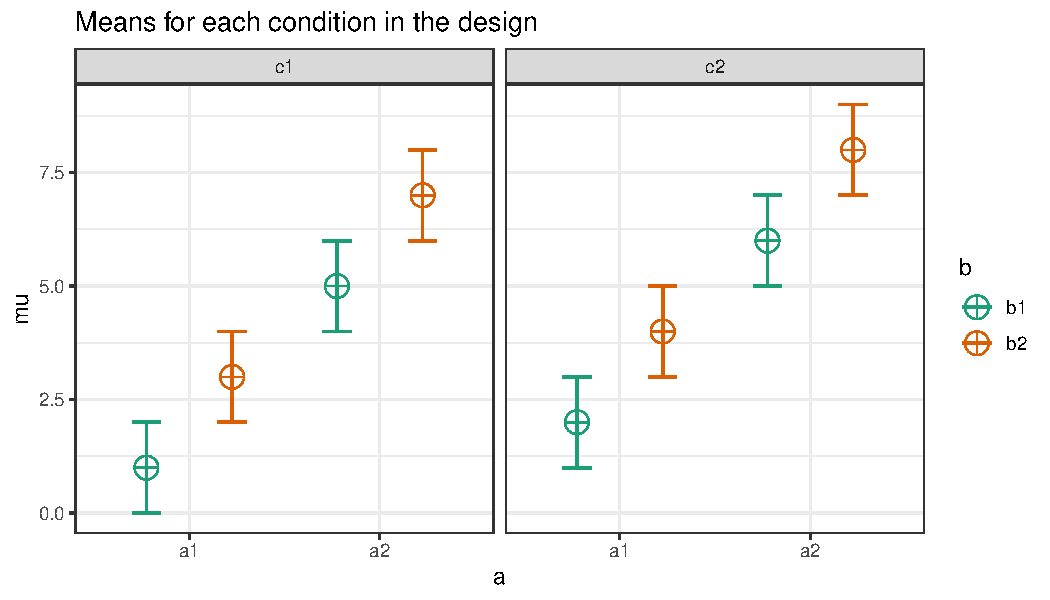
\includegraphics{SuperpowerValidation_files/figure-latex/unnamed-chunk-2-1.pdf}

\begin{Shaded}
\begin{Highlighting}[]
\NormalTok{alpha_level <-}\StringTok{ }\FloatTok{0.05}
\CommentTok{# You should think carefully about how to justify your alpha level.}
\CommentTok{# We will give some examples later, but for now, use 0.05.}
\KeywordTok{ANOVA_power}\NormalTok{(design_result, }\DataTypeTok{alpha_level =}\NormalTok{ alpha_level, }\DataTypeTok{nsims =}\NormalTok{ nsims)}
\end{Highlighting}
\end{Shaded}

\begin{verbatim}
## Power and Effect sizes for ANOVA tests
##                 power effect_size
## anova_condition    66     0.03461
## 
## Power and Effect sizes for contrasts
##                                   power effect_size
## p_condition_control_condition_pet    66      0.3465
\end{verbatim}

The result shows that we have exactly the same power for the ANOVA, as we have for the \emph{t}-test. This is because when there are only two groups, these tests are mathematically identical. In a study with 100 participants, we would have quite low power (around 67.7\%). An ANOVA with 2 groups is identical to a \emph{t}-test. For our example, Cohen's d (the standardized mean difference) is 2.2/6.4, or d = 0.34375 for the difference between the control condition and pets, which we can use to easily compute the expected power for these simple comparisons using the pwr package.

\begin{Shaded}
\begin{Highlighting}[]
\KeywordTok{pwr.t.test}\NormalTok{(}\DataTypeTok{d =} \FloatTok{2.2}\OperatorTok{/}\FloatTok{6.4}\NormalTok{,}
           \DataTypeTok{n =} \DecValTok{100}\NormalTok{,}
           \DataTypeTok{sig.level =} \FloatTok{0.05}\NormalTok{,}
           \DataTypeTok{type=}\StringTok{"two.sample"}\NormalTok{,}
           \DataTypeTok{alternative=}\StringTok{"two.sided"}\NormalTok{)}\OperatorTok{$}\NormalTok{power}
\end{Highlighting}
\end{Shaded}

\begin{verbatim}
## [1] 0.6768572
\end{verbatim}

We can also directly compute Cohen's f from Cohen's d for two groups, as Cohen (1988) describes, because f = 1/2d. So f = 0.5*0.34375 = 0.171875. And indeed, power analysis using the pwr package yields the same result using the pwr.anova.test as the power.t.test.

\begin{Shaded}
\begin{Highlighting}[]
\NormalTok{K <-}\StringTok{ }\DecValTok{2}
\NormalTok{n <-}\StringTok{ }\DecValTok{100}
\NormalTok{f <-}\StringTok{ }\FloatTok{0.171875}
\KeywordTok{pwr.anova.test}\NormalTok{(}\DataTypeTok{n =}\NormalTok{ n,}
               \DataTypeTok{k =}\NormalTok{ K,}
               \DataTypeTok{f =}\NormalTok{ f,}
               \DataTypeTok{sig.level =}\NormalTok{ alpha_level)}\OperatorTok{$}\NormalTok{power}
\end{Highlighting}
\end{Shaded}

\begin{verbatim}
## [1] 0.6768572
\end{verbatim}

This analysis tells us that running the study with 100 participants in each condition is too likely to \emph{not} yield a significant test result, even if our expected pattern of differences is true. This is not optimal.

Let's mathematically explore which pattern of means we would need to expect to habe 90\% power for the ANOVA with 50 participants in each group. We can use the pwr package in R to compute a sensitivity analysis that tells us the effect size, in Cohen's f, that we are able to detect with 3 groups and 50 partiicpants in each group, in order to achive 90\% power with an alpha level of 5\%.

\begin{Shaded}
\begin{Highlighting}[]
\NormalTok{K <-}\StringTok{ }\DecValTok{2}
\NormalTok{n <-}\StringTok{ }\DecValTok{100}
\NormalTok{sd <-}\StringTok{ }\FloatTok{6.4}
\NormalTok{r <-}\StringTok{ }\DecValTok{0}
\CommentTok{#Calculate f when running simulation}
\NormalTok{f <-}\StringTok{ }\KeywordTok{pwr.anova.test}\NormalTok{(}\DataTypeTok{n =}\NormalTok{ n,}
                    \DataTypeTok{k =}\NormalTok{ K,}
                    \DataTypeTok{power =} \FloatTok{0.9}\NormalTok{,}
                    \DataTypeTok{sig.level =}\NormalTok{ alpha_level)}\OperatorTok{$}\NormalTok{f}
\NormalTok{f}
\end{Highlighting}
\end{Shaded}

\begin{verbatim}
## [1] 0.2303587
\end{verbatim}

This sensitivity analysis shows we have 90\% power in our planned design to detect effects of Cohen's f of 0.2303587. Benchmarks by Cohen (1988) for small, medium, and large Cohen's f values are 0.1, 0.25, and 0.4, which correspond to eta-squared values of small (.0099), medium (.0588), and large (.1379), in line with d = .2, .5, or .8. So, at least based on these benchmarks, we have 90\% power to detect effects that are slightly below a medium effect benchmark.

\begin{Shaded}
\begin{Highlighting}[]
\NormalTok{f2 <-}\StringTok{ }\NormalTok{f}\OperatorTok{^}\DecValTok{2}
\NormalTok{ES <-}\StringTok{ }\NormalTok{f2}\OperatorTok{/}\NormalTok{(f2}\OperatorTok{+}\DecValTok{1}\NormalTok{)}
\NormalTok{ES}
\end{Highlighting}
\end{Shaded}

\begin{verbatim}
## [1] 0.0503911
\end{verbatim}

Expressed in eta-squared, we can detect values of eta-squared = 0.05 or larger.

\begin{Shaded}
\begin{Highlighting}[]
\NormalTok{mu <-}\StringTok{ }\KeywordTok{mu_from_ES}\NormalTok{(}\DataTypeTok{K =}\NormalTok{ K, }\DataTypeTok{ES =}\NormalTok{ ES)}
\NormalTok{mu <-}\StringTok{ }\NormalTok{mu }\OperatorTok{*}\StringTok{ }\NormalTok{sd}
\NormalTok{mu}
\end{Highlighting}
\end{Shaded}

\begin{verbatim}
## [1] -1.474295  1.474295
\end{verbatim}

We can compute a pattern of means, given a standard deviation of 6.4, that would give us an effect size of f = 0.23, or eta-squared of 0.05. We should be able to accomplish this is the means are -1.474295 and 1.474295. We can use these values to confirm the ANOVA has 90\% power.

\begin{Shaded}
\begin{Highlighting}[]
\NormalTok{design_result <-}\StringTok{ }\KeywordTok{ANOVA_design}\NormalTok{(}\DataTypeTok{design =}\NormalTok{ string,}
                   \DataTypeTok{n =}\NormalTok{ n, }
                   \DataTypeTok{mu =}\NormalTok{ mu, }
                   \DataTypeTok{sd =}\NormalTok{ sd, }
                   \DataTypeTok{labelnames =}\NormalTok{ labelnames)}
\end{Highlighting}
\end{Shaded}

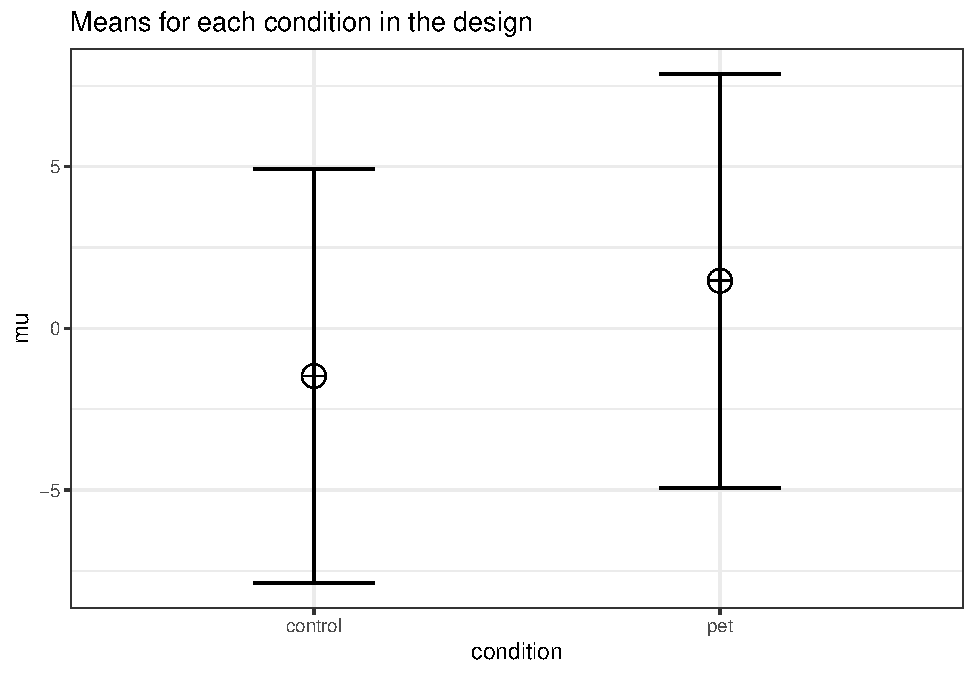
\includegraphics{SuperpowerValidation_files/figure-latex/unnamed-chunk-8-1.pdf}

\begin{Shaded}
\begin{Highlighting}[]
\KeywordTok{ANOVA_power}\NormalTok{(design_result, }\DataTypeTok{alpha_level =}\NormalTok{ alpha_level, }\DataTypeTok{nsims =}\NormalTok{ nsims)}
\end{Highlighting}
\end{Shaded}

\begin{verbatim}
## Power and Effect sizes for ANOVA tests
##                 power effect_size
## anova_condition    88      0.0511
## 
## Power and Effect sizes for contrasts
##                                   power effect_size
## p_condition_control_condition_pet    88      0.4444
\end{verbatim}

The simulation confirms that for the \emph{F}-test for the ANOVA we have 90\% power. This is also what g*power tells us what would happen based on a post-hoc power analysis with an f of 0.2303587, 2 groups, 200 participants in total (100 in each between subject condition), and an alpha of 5\%.

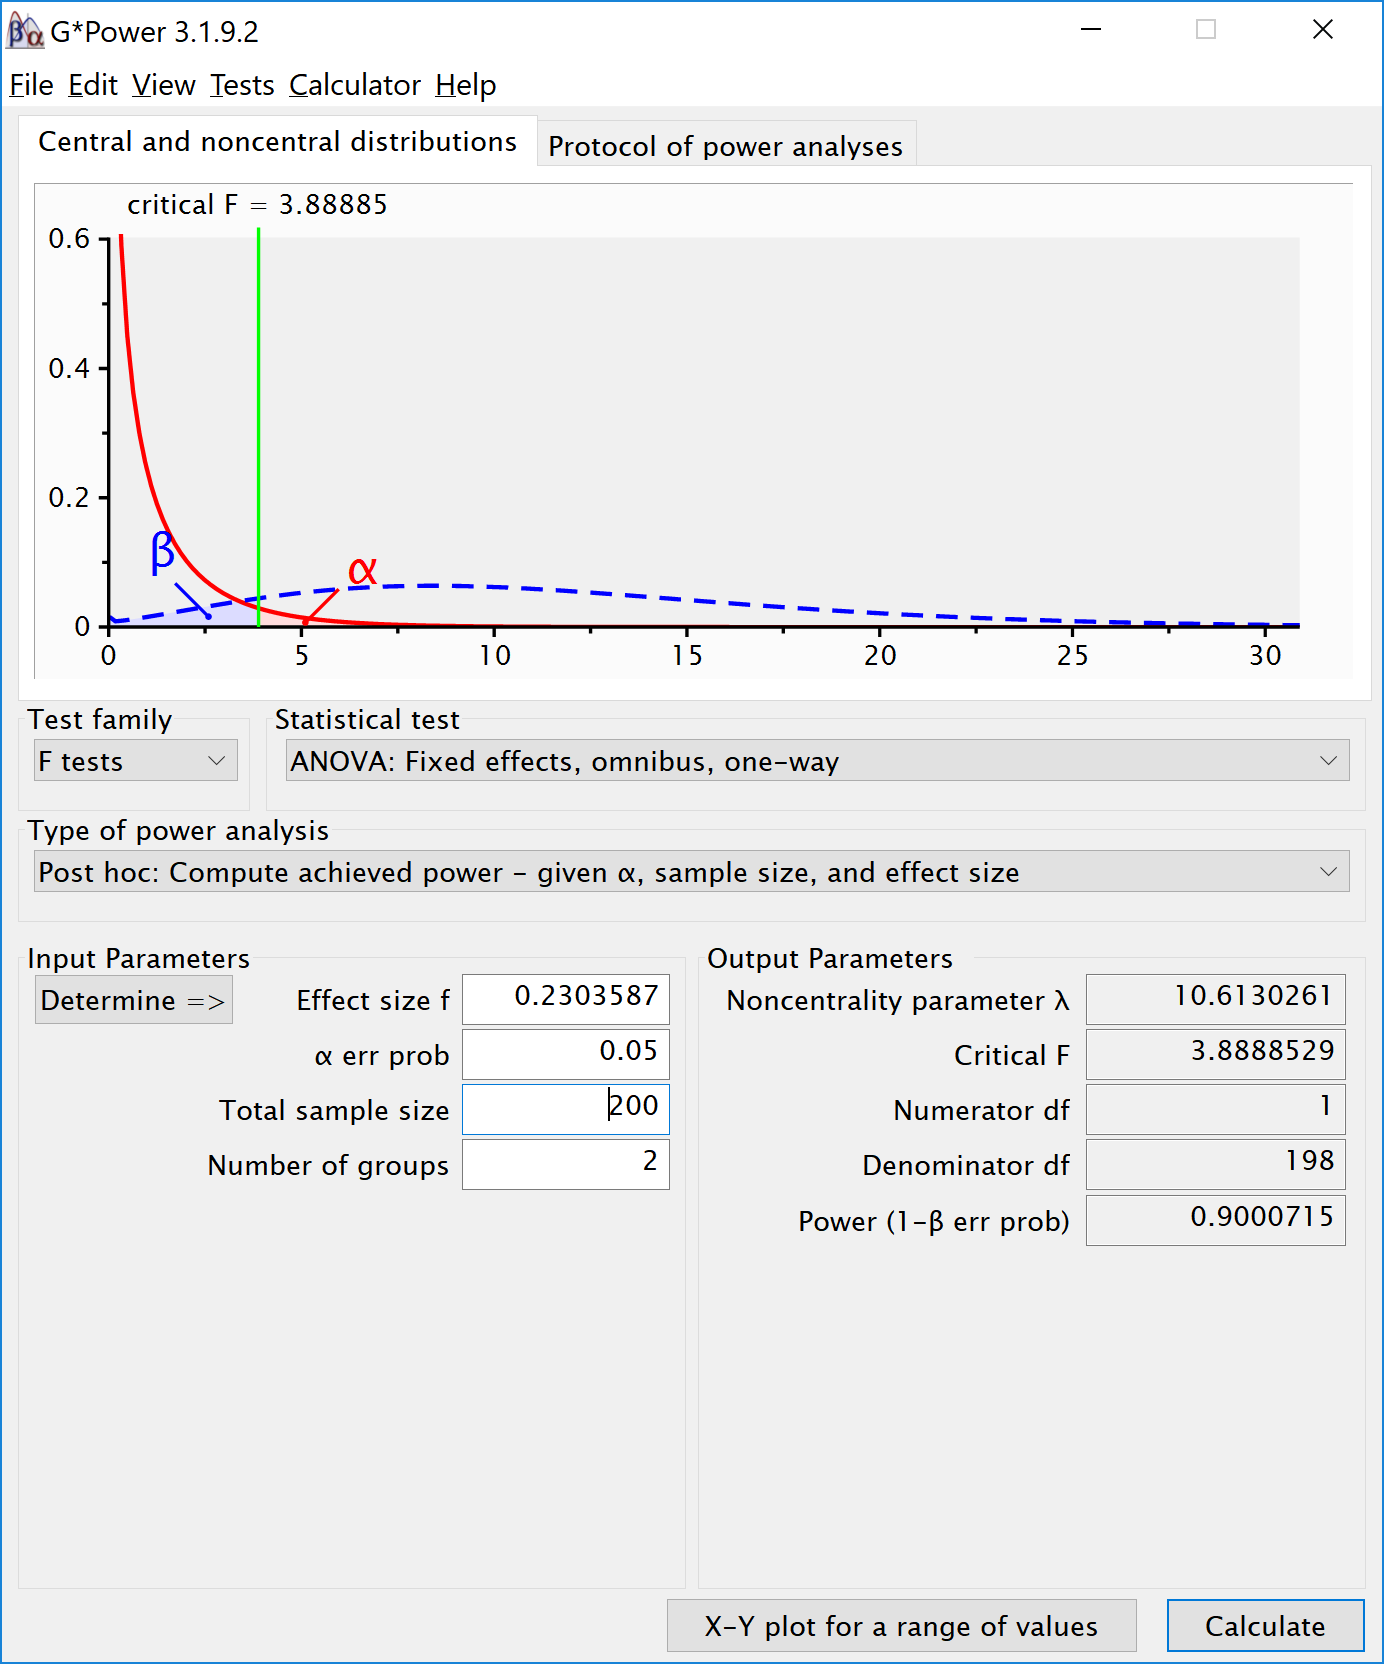
\includegraphics{screenshots/gpower_8.png}
If we return to our expected means, how many participants do we need for sufficient power? Given the expected difference and standard deviation, d = 0.34375, and f = 0.171875. We can perform an a-priori power analysis for this simple case, which tells us we need 179 participants in each group (we can't split people in parts, and thus always round a power analysis upward), or 358 in total.

\begin{Shaded}
\begin{Highlighting}[]
\NormalTok{K <-}\StringTok{ }\DecValTok{2}
\NormalTok{power <-}\StringTok{ }\FloatTok{0.9}
\NormalTok{f <-}\StringTok{ }\FloatTok{0.171875}
\KeywordTok{pwr.anova.test}\NormalTok{(}\DataTypeTok{power =}\NormalTok{ power,}
               \DataTypeTok{k =}\NormalTok{ K,}
               \DataTypeTok{f =}\NormalTok{ f,}
               \DataTypeTok{sig.level =}\NormalTok{ alpha_level)}
\end{Highlighting}
\end{Shaded}

\begin{verbatim}
## 
##      Balanced one-way analysis of variance power calculation 
## 
##               k = 2
##               n = 178.8104
##               f = 0.171875
##       sig.level = 0.05
##           power = 0.9
## 
## NOTE: n is number in each group
\end{verbatim}

If we re-run the simulation with this sample size, we indeed have 90\% power.

\begin{Shaded}
\begin{Highlighting}[]
\NormalTok{string <-}\StringTok{ "2b"}
\NormalTok{n <-}\StringTok{ }\DecValTok{179}
\NormalTok{mu <-}\StringTok{ }\KeywordTok{c}\NormalTok{(}\DecValTok{24}\NormalTok{, }\FloatTok{26.2}\NormalTok{)}
\CommentTok{# Enter means in the order that matches the labels below.}
\CommentTok{# In this case, control, pet. }
\NormalTok{sd <-}\StringTok{ }\FloatTok{6.4}
\NormalTok{labelnames <-}\StringTok{ }\KeywordTok{c}\NormalTok{(}\StringTok{"condition"}\NormalTok{, }\StringTok{"control"}\NormalTok{, }\StringTok{"pet"}\NormalTok{) }\CommentTok{#}
\CommentTok{# the label names should be in the order of the means specified above.}
\NormalTok{design_result <-}\StringTok{ }\KeywordTok{ANOVA_design}\NormalTok{(}\DataTypeTok{design =}\NormalTok{ string,}
                   \DataTypeTok{n =}\NormalTok{ n, }
                   \DataTypeTok{mu =}\NormalTok{ mu, }
                   \DataTypeTok{sd =}\NormalTok{ sd, }
                   \DataTypeTok{labelnames =}\NormalTok{ labelnames)}
\end{Highlighting}
\end{Shaded}

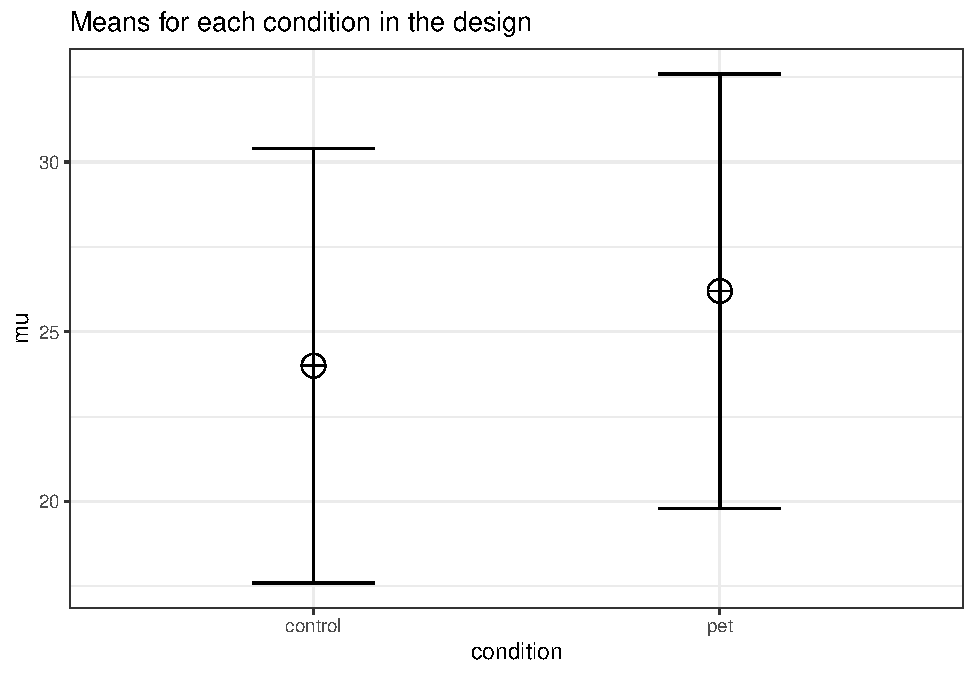
\includegraphics{SuperpowerValidation_files/figure-latex/unnamed-chunk-10-1.pdf}

\begin{Shaded}
\begin{Highlighting}[]
\NormalTok{alpha_level <-}\StringTok{ }\FloatTok{0.05}
\NormalTok{power_result <-}\StringTok{ }\KeywordTok{ANOVA_power}\NormalTok{(design_result, }\DataTypeTok{alpha_level =}\NormalTok{ alpha_level, }\DataTypeTok{nsims =}\NormalTok{ nsims)}
\end{Highlighting}
\end{Shaded}

\begin{verbatim}
## Power and Effect sizes for ANOVA tests
##                 power effect_size
## anova_condition    85     0.03191
## 
## Power and Effect sizes for contrasts
##                                   power effect_size
## p_condition_control_condition_pet    85      0.3474
\end{verbatim}

We stored the result from the power analysis in an object. This allows us to request plots (which are not printed automatically) showing the \emph{p}-value distribution. If we request power\_result\$plot1 we get the p-value distribution for the ANOVA:

\begin{Shaded}
\begin{Highlighting}[]
\NormalTok{power_result}\OperatorTok{$}\NormalTok{plot1}
\end{Highlighting}
\end{Shaded}

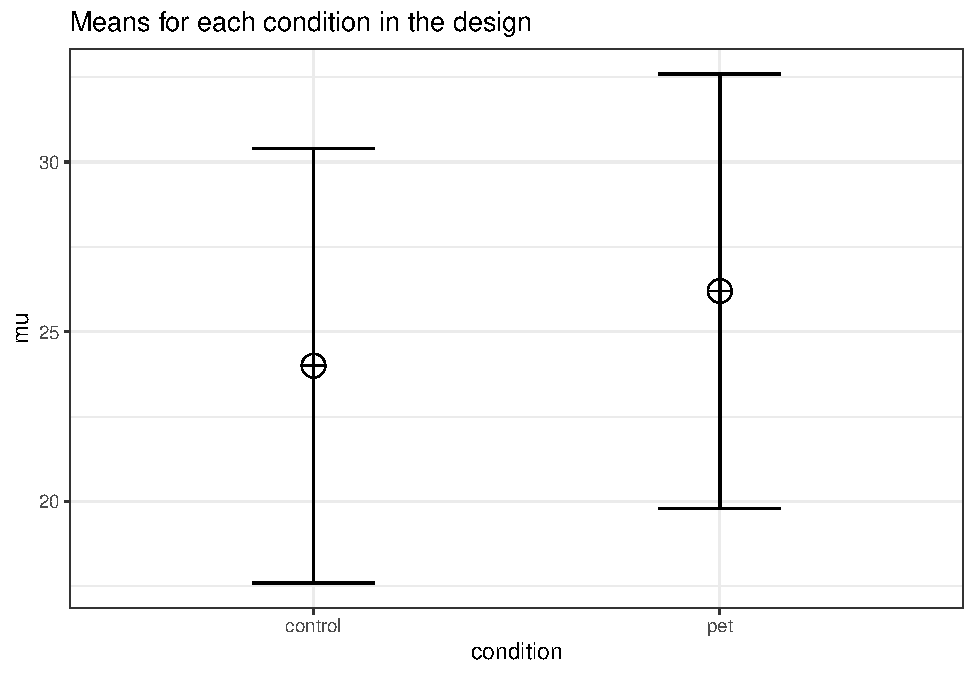
\includegraphics{SuperpowerValidation_files/figure-latex/unnamed-chunk-11-1.pdf}
If we request power\_result\$plot2 we get the p-value distribution for the paired comparisons (in this case only one):

\begin{Shaded}
\begin{Highlighting}[]
\NormalTok{power_result}\OperatorTok{$}\NormalTok{plot2}
\end{Highlighting}
\end{Shaded}

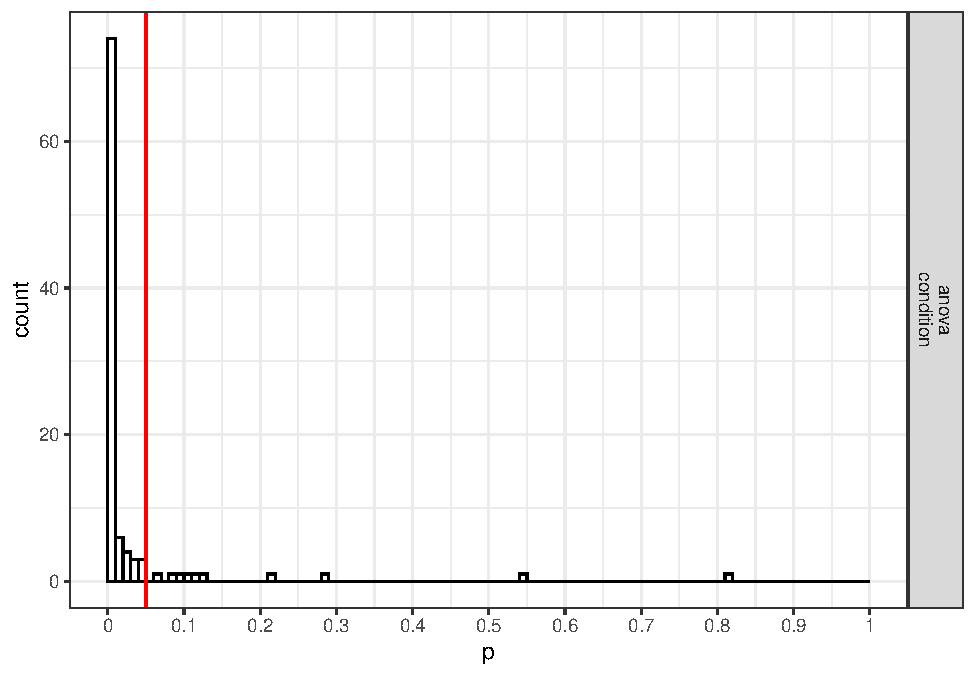
\includegraphics{SuperpowerValidation_files/figure-latex/unnamed-chunk-12-1.pdf}

\hypertarget{one-way-anova-part-2}{%
\chapter{One-way ANOVA Part 2}\label{one-way-anova-part-2}}

\hypertarget{validation-of-power-in-one-way-anova-with-brysbaert-example}{%
\section{Validation of Power in One-Way ANOVA with Brysbaert example}\label{validation-of-power-in-one-way-anova-with-brysbaert-example}}

\hypertarget{three-conditions}{%
\subsection{Three conditions}\label{three-conditions}}

Imagine we aim to design a study to test the hypothesis that giving people a pet to take care of will increase their life satisfaction. We have a control condition, a `cat' pet condition, and a `dog' pet condition. We can simulate a One-Way ANOVA with a specified alpha, sample size, and effect size, on see the statistical power we would have for the ANOVA and the follow-up comparisons. We expect all pets to increase life-satisfaction compared to the control condition. Obviously, we also expect the people who are in the `dog' pet condition to have even greater life-satisfaction than people in the `cat' pet condition. Based on work by Pavot and Diener (1993) we believe that we can expect responses on the life-satifaction scale to have a mean of approximately 24 in our population, with a standard deviation of 6.4. We expect having a pet increases life satisfaction with approximately 2.2 scale points for participants who get a cat, and 2.6 scale points for participants who get a dog. We initially consider collecting data from 150 participants in total, with 50 participants in each condition. But before we proceed with the data collection, we examine the statistical power our design would have to detect the differences we predict.

\begin{Shaded}
\begin{Highlighting}[]
\NormalTok{string <-}\StringTok{ "3b"}
\NormalTok{n <-}\StringTok{ }\DecValTok{50}
\CommentTok{# We are thinking of running 50 peope in each condition}
\NormalTok{mu <-}\StringTok{ }\KeywordTok{c}\NormalTok{(}\DecValTok{24}\NormalTok{, }\FloatTok{26.2}\NormalTok{, }\FloatTok{26.6}\NormalTok{)}
\CommentTok{# Enter means in the order that matches the labels below.}
\CommentTok{# In this case, control, cat, dog. }
\NormalTok{sd <-}\StringTok{ }\FloatTok{6.4}
\NormalTok{labelnames <-}\StringTok{ }\KeywordTok{c}\NormalTok{(}\StringTok{"condition"}\NormalTok{, }\StringTok{"control"}\NormalTok{, }\StringTok{"cat"}\NormalTok{, }\StringTok{"dog"}\NormalTok{) }\CommentTok{#}
\CommentTok{# the label names should be in the order of the means specified above.}
\NormalTok{design_result <-}\StringTok{ }\KeywordTok{ANOVA_design}\NormalTok{(}\DataTypeTok{design =}\NormalTok{ string,}
                   \DataTypeTok{n =}\NormalTok{ n, }
                   \DataTypeTok{mu =}\NormalTok{ mu, }
                   \DataTypeTok{sd =}\NormalTok{ sd, }
                   \DataTypeTok{labelnames =}\NormalTok{ labelnames)}
\end{Highlighting}
\end{Shaded}

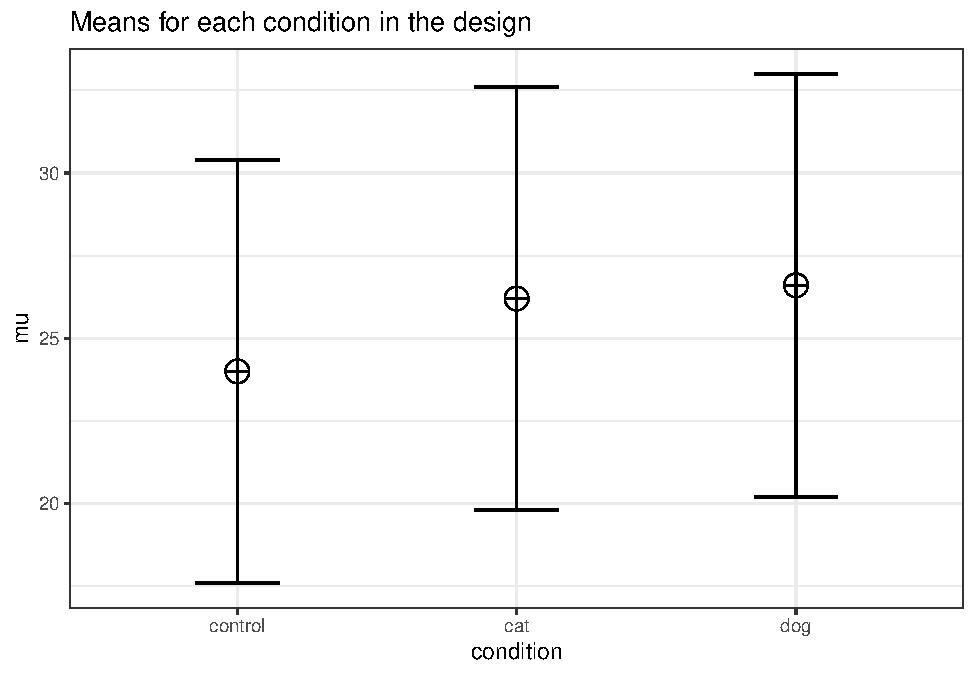
\includegraphics{SuperpowerValidation_files/figure-latex/unnamed-chunk-14-1.pdf}

\begin{Shaded}
\begin{Highlighting}[]
\NormalTok{alpha_level <-}\StringTok{ }\FloatTok{0.05}
\CommentTok{# You should think carefully about how to justify your alpha level.}
\CommentTok{# We will give some examples later, but for now, use 0.05.}
\KeywordTok{ANOVA_power}\NormalTok{(design_result, }\DataTypeTok{alpha_level =}\NormalTok{ alpha_level, }\DataTypeTok{nsims =}\NormalTok{ nsims)}
\end{Highlighting}
\end{Shaded}

\begin{verbatim}
## Power and Effect sizes for ANOVA tests
##                 power effect_size
## anova_condition    53     0.05078
## 
## Power and Effect sizes for contrasts
##                                   power effect_size
## p_condition_control_condition_cat    44      0.3614
## p_condition_control_condition_dog    61      0.4644
## p_condition_cat_condition_dog         5      0.1008
\end{verbatim}

\begin{Shaded}
\begin{Highlighting}[]
\CommentTok{#should yield}
\CommentTok{#0.3983064}
\CommentTok{#0.5205162}
\CommentTok{#0.06104044}
\end{Highlighting}
\end{Shaded}

The result shows that you would have quite low power with 50 participants, both for the overall ANOVA (just around 50\% power), as for the follow up comparisons (approximately 40\% power for the control vs cat condition, around 50\% for the control vs dogs condition, and a really low power (around 6\%, just above the Type 1 error rate of 5\%) for the expected difference between cats and dogs.

\hypertarget{power-for-simple-effects}{%
\section{Power for simple effects}\label{power-for-simple-effects}}

We are typically not just interested in the ANOVA, but also in follow up comparisons. In this case, we would perform a \emph{t}-test comparing the control condition against the cat and dog condition, and we would compare the cat and dog conditions against each other, in independent \emph{t}-tests.

For our example, Cohen's d (the standardized mean difference) is 2.2/6.4, or d = 0.34375 for the difference between the control condition and cats, 2.6/6.4 of d = 0.40625 for the difference between the control condition and dogs, and 0.4/6.4 or d = 0.0625 for the difference between cats and dogs as pets.

We can easily compute the expected power for these simple comparisons using the pwr package.

\begin{Shaded}
\begin{Highlighting}[]
\KeywordTok{pwr.t.test}\NormalTok{(}\DataTypeTok{d =} \FloatTok{2.2}\OperatorTok{/}\FloatTok{6.4}\NormalTok{,}
           \DataTypeTok{n =} \DecValTok{50}\NormalTok{,}
           \DataTypeTok{sig.level =} \FloatTok{0.05}\NormalTok{,}
           \DataTypeTok{type=}\StringTok{"two.sample"}\NormalTok{,}
           \DataTypeTok{alternative=}\StringTok{"two.sided"}\NormalTok{)}\OperatorTok{$}\NormalTok{power}
\end{Highlighting}
\end{Shaded}

\begin{verbatim}
## [1] 0.3983064
\end{verbatim}

\begin{Shaded}
\begin{Highlighting}[]
\KeywordTok{pwr.t.test}\NormalTok{(}\DataTypeTok{d =} \FloatTok{2.6}\OperatorTok{/}\FloatTok{6.4}\NormalTok{,}
           \DataTypeTok{n =} \DecValTok{50}\NormalTok{,}
           \DataTypeTok{sig.level =} \FloatTok{0.05}\NormalTok{,}
           \DataTypeTok{type=}\StringTok{"two.sample"}\NormalTok{,}
           \DataTypeTok{alternative=}\StringTok{"two.sided"}\NormalTok{)}\OperatorTok{$}\NormalTok{power}
\end{Highlighting}
\end{Shaded}

\begin{verbatim}
## [1] 0.5205162
\end{verbatim}

\begin{Shaded}
\begin{Highlighting}[]
\KeywordTok{pwr.t.test}\NormalTok{(}\DataTypeTok{d =} \FloatTok{0.4}\OperatorTok{/}\FloatTok{6.4}\NormalTok{,}
           \DataTypeTok{n =} \DecValTok{50}\NormalTok{,}
           \DataTypeTok{sig.level =} \FloatTok{0.05}\NormalTok{,}
           \DataTypeTok{type=}\StringTok{"two.sample"}\NormalTok{,}
           \DataTypeTok{alternative=}\StringTok{"two.sided"}\NormalTok{)}\OperatorTok{$}\NormalTok{power}
\end{Highlighting}
\end{Shaded}

\begin{verbatim}
## [1] 0.06104044
\end{verbatim}

This analysis tells us that running the study with 50 participants in each condition is more likely to \emph{not} yield a significant test result, even if our expected pattern of differences is true, than that we will observe a \emph{p}-value smaller than our alpha level. This is not optimal.

Let's mathematically explore which pattern of means we would need to expect to habe 90\% power for the ANOVA with 50 participants in each group. We can use the pwr package in R to compute a sensitivity analysis that tells us the effect size, in Cohen's f, that we are able to detect with 3 groups and 50 partiicpants in each group, in order to achive 90\% power with an alpha level of 5\%.

\begin{Shaded}
\begin{Highlighting}[]
\NormalTok{K <-}\StringTok{ }\DecValTok{3}
\NormalTok{n <-}\StringTok{ }\DecValTok{50}
\NormalTok{sd <-}\StringTok{ }\FloatTok{6.4}
\NormalTok{r <-}\StringTok{ }\DecValTok{0}
\CommentTok{#Calculate f when running simulation}
\NormalTok{f <-}\StringTok{ }\KeywordTok{pwr.anova.test}\NormalTok{(}\DataTypeTok{n =}\NormalTok{ n,}
                    \DataTypeTok{k =}\NormalTok{ K,}
                    \DataTypeTok{power =} \FloatTok{0.9}\NormalTok{,}
                    \DataTypeTok{sig.level =}\NormalTok{ alpha_level)}\OperatorTok{$}\NormalTok{f}
\NormalTok{f}
\end{Highlighting}
\end{Shaded}

\begin{verbatim}
## [1] 0.2934417
\end{verbatim}

This sensitivity analysis shows we have 90\% power in our planned design to detect effects of Cohen's f of 0.2934417. Benchmarks by Cohen (1988) for small, medium, and large Cohen's f values are 0.1, 0.25, and 0.4, which correspond to eta-squared values of small (.0099), medium (.0588), and large (.1379), in line with d = .2, .5, or .8. So, at least based on these benchmarks, we have 90\% power to detect effects that are somewhat sizeable.

\begin{Shaded}
\begin{Highlighting}[]
\NormalTok{f2 <-}\StringTok{ }\NormalTok{f}\OperatorTok{^}\DecValTok{2}
\NormalTok{ES <-}\StringTok{ }\NormalTok{f2}\OperatorTok{/}\NormalTok{(f2}\OperatorTok{+}\DecValTok{1}\NormalTok{)}
\NormalTok{ES}
\end{Highlighting}
\end{Shaded}

\begin{verbatim}
## [1] 0.07928127
\end{verbatim}

Expressed in eta-squared, we can detect values of eta-squared = 0.0793 or larger.

\begin{Shaded}
\begin{Highlighting}[]
\NormalTok{mu <-}\StringTok{ }\KeywordTok{mu_from_ES}\NormalTok{(}\DataTypeTok{K =}\NormalTok{ K, }\DataTypeTok{ES =}\NormalTok{ ES)}
\NormalTok{mu <-}\StringTok{ }\NormalTok{mu }\OperatorTok{*}\StringTok{ }\NormalTok{sd}
\NormalTok{mu}
\end{Highlighting}
\end{Shaded}

\begin{verbatim}
## [1] -2.300104  0.000000  2.300104
\end{verbatim}

We can compute a pattern of means, given a standard deviation of 6.4, that would give us an effect size of f = 0.2934, or eta-squared of 0.0793. We should be able to accomplish this is the means are -2.300104, 0.000000, and 2.300104. We can use these values to confirm the ANOVA has 90\% power.

\begin{Shaded}
\begin{Highlighting}[]
\NormalTok{design_result <-}\StringTok{ }\KeywordTok{ANOVA_design}\NormalTok{(}\DataTypeTok{design =}\NormalTok{ string,}
                   \DataTypeTok{n =}\NormalTok{ n, }
                   \DataTypeTok{mu =}\NormalTok{ mu, }
                   \DataTypeTok{sd =}\NormalTok{ sd, }
                   \DataTypeTok{labelnames =}\NormalTok{ labelnames)}
\end{Highlighting}
\end{Shaded}

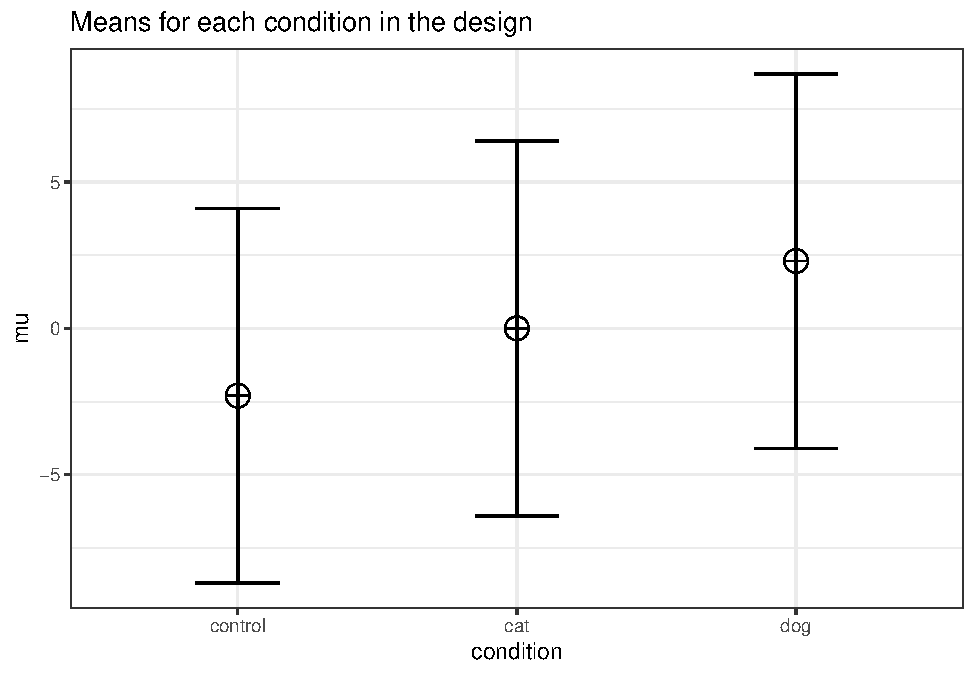
\includegraphics{SuperpowerValidation_files/figure-latex/unnamed-chunk-19-1.pdf}

\begin{Shaded}
\begin{Highlighting}[]
\KeywordTok{ANOVA_power}\NormalTok{(design_result, }\DataTypeTok{alpha_level =}\NormalTok{ alpha_level, }\DataTypeTok{nsims =}\NormalTok{ nsims)}
\end{Highlighting}
\end{Shaded}

\begin{verbatim}
## Power and Effect sizes for ANOVA tests
##                 power effect_size
## anova_condition    95     0.09547
## 
## Power and Effect sizes for contrasts
##                                   power effect_size
## p_condition_control_condition_cat    46      0.4072
## p_condition_control_condition_dog    98      0.7647
## p_condition_cat_condition_dog        39      0.3475
\end{verbatim}

The simulation confirms that for the \emph{F}-test for the ANOVA we have 90\% power. This is also what g*power tells us what would happen based on a post-hoc power analysis with an f of 0.2934417, 3 groups, 150 participants in total (50 in each between subject condition), and an alpha of 5\%.

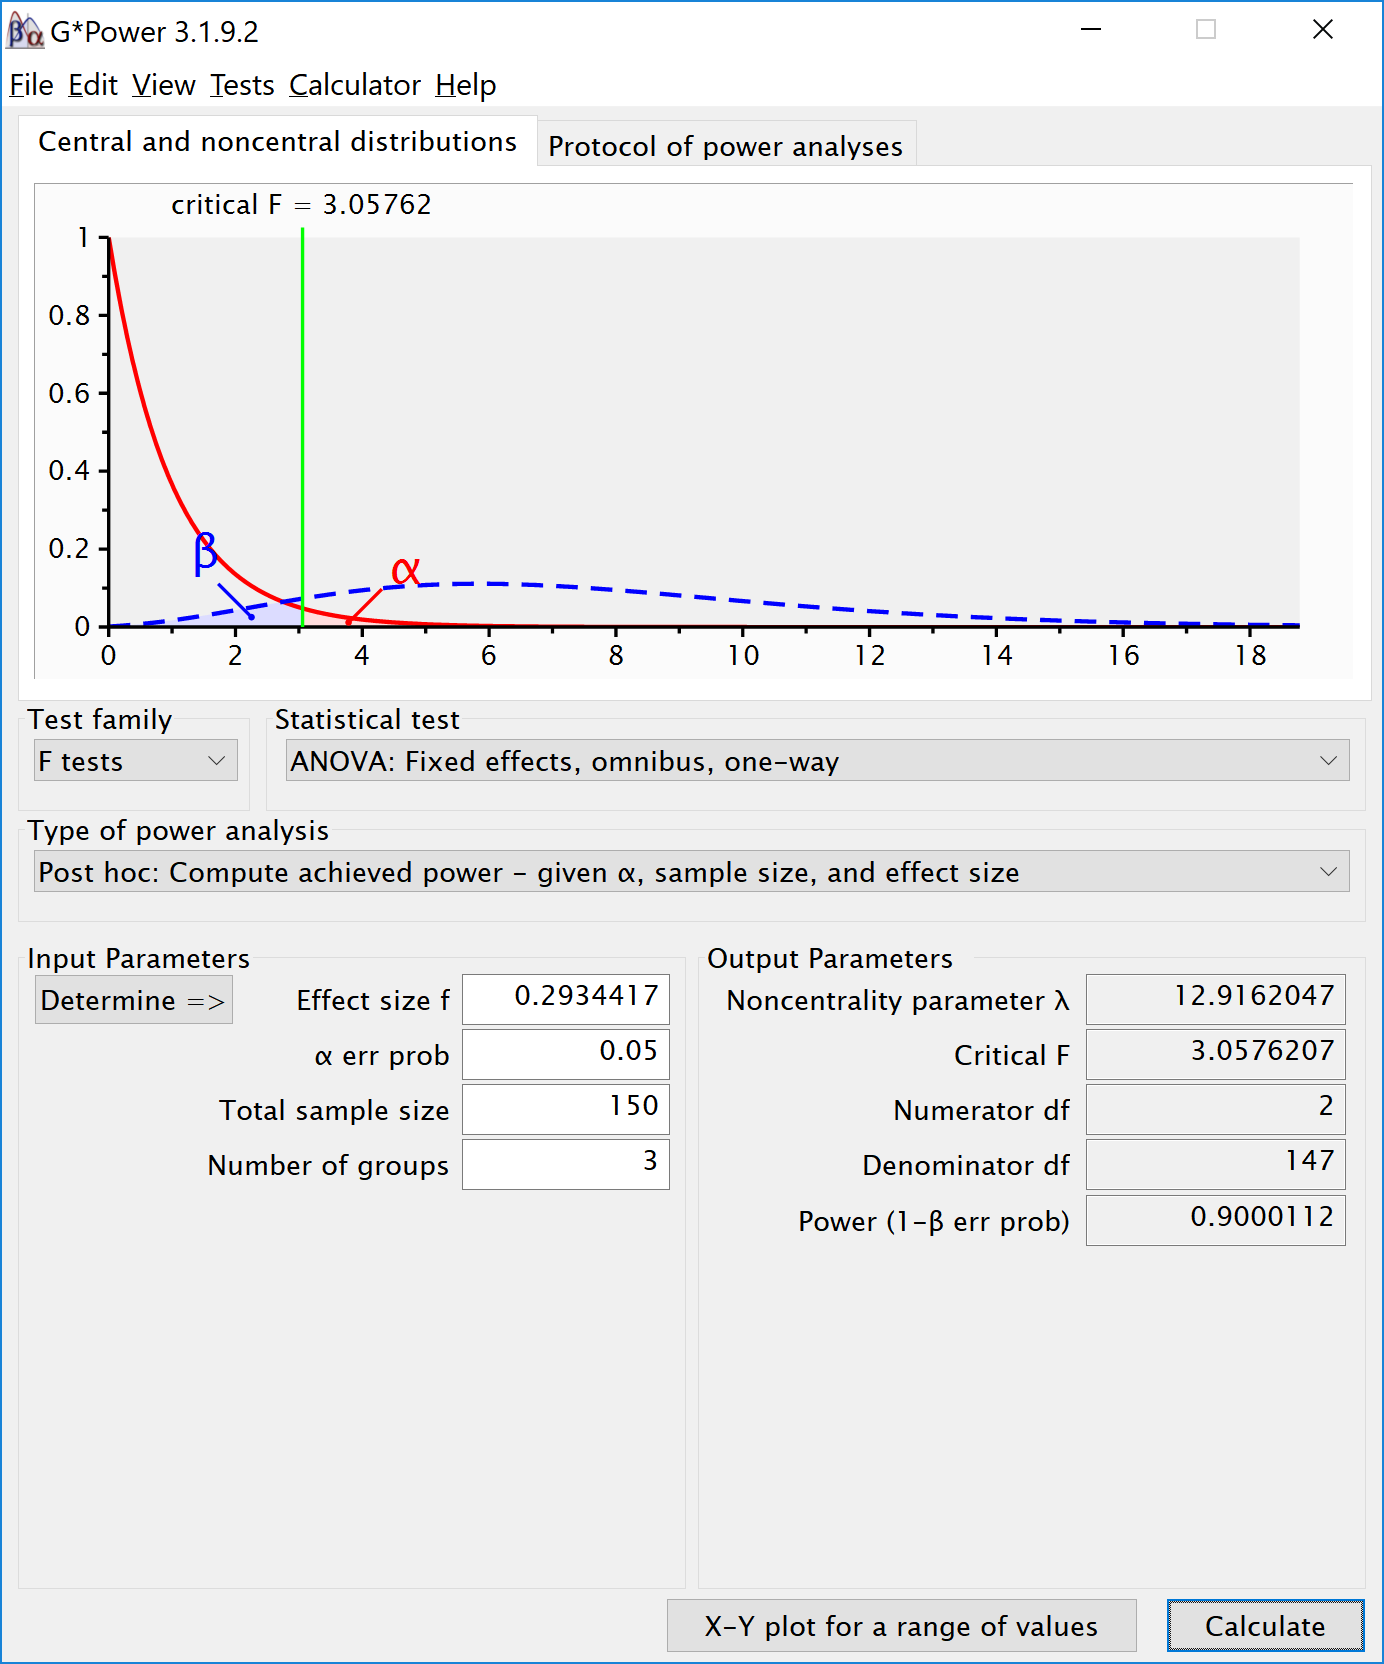
\includegraphics{screenshots/gpower_7.png}

We can also compute the power for the ANOVA and simple effects in R with the pwr package. The calculated effect sizes and power match those from the simulation.

\begin{Shaded}
\begin{Highlighting}[]
\NormalTok{K <-}\StringTok{ }\DecValTok{3}
\NormalTok{n <-}\StringTok{ }\DecValTok{50}
\NormalTok{sd <-}\StringTok{ }\FloatTok{6.4}
\NormalTok{f <-}\StringTok{ }\FloatTok{0.2934417}
\KeywordTok{pwr.anova.test}\NormalTok{(}\DataTypeTok{n =}\NormalTok{ n,}
               \DataTypeTok{k =}\NormalTok{ K,}
               \DataTypeTok{f =}\NormalTok{ f,}
               \DataTypeTok{sig.level =}\NormalTok{ alpha_level)}\OperatorTok{$}\NormalTok{power}
\end{Highlighting}
\end{Shaded}

\begin{verbatim}
## [1] 0.9000112
\end{verbatim}

\begin{Shaded}
\begin{Highlighting}[]
\NormalTok{d <-}\StringTok{ }\FloatTok{2.300104}\OperatorTok{/}\FloatTok{6.4}
\NormalTok{d}
\end{Highlighting}
\end{Shaded}

\begin{verbatim}
## [1] 0.3593912
\end{verbatim}

\begin{Shaded}
\begin{Highlighting}[]
\KeywordTok{pwr.t.test}\NormalTok{(}\DataTypeTok{d =} \FloatTok{2.300104}\OperatorTok{/}\FloatTok{6.4}\NormalTok{,}
           \DataTypeTok{n =} \DecValTok{50}\NormalTok{,}
           \DataTypeTok{sig.level =} \FloatTok{0.05}\NormalTok{,}
           \DataTypeTok{type=}\StringTok{"two.sample"}\NormalTok{,}
           \DataTypeTok{alternative=}\StringTok{"two.sided"}\NormalTok{)}\OperatorTok{$}\NormalTok{power}
\end{Highlighting}
\end{Shaded}

\begin{verbatim}
## [1] 0.4284243
\end{verbatim}

\begin{Shaded}
\begin{Highlighting}[]
\NormalTok{d <-}\StringTok{ }\DecValTok{2}\OperatorTok{*}\FloatTok{2.300104}\OperatorTok{/}\FloatTok{6.4}
\NormalTok{d}
\end{Highlighting}
\end{Shaded}

\begin{verbatim}
## [1] 0.7187825
\end{verbatim}

\begin{Shaded}
\begin{Highlighting}[]
\KeywordTok{pwr.t.test}\NormalTok{(}\DataTypeTok{d =}\NormalTok{ d,}
           \DataTypeTok{n =} \DecValTok{50}\NormalTok{,}
           \DataTypeTok{sig.level =} \FloatTok{0.05}\NormalTok{,}
           \DataTypeTok{type=}\StringTok{"two.sample"}\NormalTok{,}
           \DataTypeTok{alternative=}\StringTok{"two.sided"}\NormalTok{)}\OperatorTok{$}\NormalTok{power}
\end{Highlighting}
\end{Shaded}

\begin{verbatim}
## [1] 0.9450353
\end{verbatim}

We can also compare the results against the analytic solution by Aberson (2019).

First, load the function for a 3-way ANOVA.

\begin{Shaded}
\begin{Highlighting}[]
\NormalTok{anova1f_}\DecValTok{3}\NormalTok{<-}\ControlFlowTok{function}\NormalTok{(}\DataTypeTok{m1=}\OtherTok{NULL}\NormalTok{,}\DataTypeTok{m2=}\OtherTok{NULL}\NormalTok{,}\DataTypeTok{m3=}\OtherTok{NULL}\NormalTok{,}\DataTypeTok{s1=}\OtherTok{NULL}\NormalTok{,}\DataTypeTok{s2=}\OtherTok{NULL}\NormalTok{,}\DataTypeTok{s3=}\OtherTok{NULL}\NormalTok{,}\DataTypeTok{n1=}\OtherTok{NULL}\NormalTok{,}\DataTypeTok{n2=}\OtherTok{NULL}\NormalTok{,}\DataTypeTok{n3=}\OtherTok{NULL}\NormalTok{,}\DataTypeTok{alpha=}\NormalTok{.}\DecValTok{05}\NormalTok{)\{}
\NormalTok{x<-stats}\OperatorTok{::}\KeywordTok{rnorm}\NormalTok{(n1,m1,s1)}
\NormalTok{X<-x}
\NormalTok{MEAN<-m1}
\NormalTok{SD<-s1}
\NormalTok{Z <-}\StringTok{ }\NormalTok{(((X }\OperatorTok{-}\StringTok{ }\KeywordTok{mean}\NormalTok{(X, }\DataTypeTok{na.rm =} \OtherTok{TRUE}\NormalTok{))}\OperatorTok{/}\NormalTok{stats}\OperatorTok{::}\KeywordTok{sd}\NormalTok{(X, }\DataTypeTok{na.rm =} \OtherTok{TRUE}\NormalTok{))) }\OperatorTok{*}\StringTok{ }\NormalTok{SD}
\NormalTok{y<-MEAN }\OperatorTok{+}\StringTok{ }\NormalTok{Z}
\NormalTok{group<-}\KeywordTok{rep}\NormalTok{(}\StringTok{"A1"}\NormalTok{,n1)}
\NormalTok{l1<-}\KeywordTok{data.frame}\NormalTok{(y, group)}
\NormalTok{x<-stats}\OperatorTok{::}\KeywordTok{rnorm}\NormalTok{(n2,m2,s2)}
\NormalTok{X<-x}
\NormalTok{MEAN<-m2}
\NormalTok{SD<-s2}
\NormalTok{Z <-}\StringTok{ }\NormalTok{(((X }\OperatorTok{-}\StringTok{ }\KeywordTok{mean}\NormalTok{(X, }\DataTypeTok{na.rm =} \OtherTok{TRUE}\NormalTok{))}\OperatorTok{/}\NormalTok{stats}\OperatorTok{::}\KeywordTok{sd}\NormalTok{(X, }\DataTypeTok{na.rm =} \OtherTok{TRUE}\NormalTok{))) }\OperatorTok{*}\StringTok{ }\NormalTok{SD}
\NormalTok{y<-MEAN }\OperatorTok{+}\StringTok{ }\NormalTok{Z}
\NormalTok{group<-}\KeywordTok{rep}\NormalTok{(}\StringTok{"A2"}\NormalTok{,n2)}
\NormalTok{l2<-}\KeywordTok{data.frame}\NormalTok{(y, group)}
\NormalTok{x<-stats}\OperatorTok{::}\KeywordTok{rnorm}\NormalTok{(n3,m3,s3)}
\NormalTok{X<-x}
\NormalTok{MEAN<-m3}
\NormalTok{SD<-s3}
\NormalTok{Z <-}\StringTok{ }\NormalTok{(((X }\OperatorTok{-}\StringTok{ }\KeywordTok{mean}\NormalTok{(X, }\DataTypeTok{na.rm =} \OtherTok{TRUE}\NormalTok{))}\OperatorTok{/}\NormalTok{stats}\OperatorTok{::}\KeywordTok{sd}\NormalTok{(X, }\DataTypeTok{na.rm =} \OtherTok{TRUE}\NormalTok{))) }\OperatorTok{*}\StringTok{ }\NormalTok{SD}
\NormalTok{y<-MEAN }\OperatorTok{+}\StringTok{ }\NormalTok{Z}
\NormalTok{group<-}\KeywordTok{rep}\NormalTok{(}\StringTok{"A3"}\NormalTok{,n3)}
\NormalTok{l3<-}\KeywordTok{data.frame}\NormalTok{(y, group)}
\NormalTok{simdat<-}\KeywordTok{rbind}\NormalTok{(l1,l2,l3)}
\NormalTok{anova<-stats}\OperatorTok{::}\KeywordTok{aov}\NormalTok{(y}\OperatorTok{~}\NormalTok{group, }\DataTypeTok{data=}\NormalTok{simdat)}
\NormalTok{anova<-car}\OperatorTok{::}\KeywordTok{Anova}\NormalTok{(anova, }\DataTypeTok{type=}\StringTok{"III"}\NormalTok{)}
\NormalTok{SSA<-anova[}\DecValTok{2}\NormalTok{,}\DecValTok{1}\NormalTok{] }\CommentTok{#column, row}
\NormalTok{SSwin<-anova[}\DecValTok{3}\NormalTok{,}\DecValTok{1}\NormalTok{]}
\NormalTok{dfwin<-anova[}\DecValTok{3}\NormalTok{,}\DecValTok{2}\NormalTok{]}
\NormalTok{dfbg<-anova[}\DecValTok{2}\NormalTok{,}\DecValTok{2}\NormalTok{]}
\NormalTok{eta2<-SSA}\OperatorTok{/}\NormalTok{(SSA}\OperatorTok{+}\NormalTok{SSwin)}
\NormalTok{f2<-eta2}\OperatorTok{/}\NormalTok{(}\DecValTok{1}\OperatorTok{-}\NormalTok{eta2)}
\NormalTok{lambda<-f2}\OperatorTok{*}\NormalTok{dfwin}
\NormalTok{minusalpha<-}\DecValTok{1}\OperatorTok{-}\NormalTok{alpha}
\NormalTok{Ft<-stats}\OperatorTok{::}\KeywordTok{qf}\NormalTok{(minusalpha, dfbg, dfwin)}
\NormalTok{power<-}\DecValTok{1}\OperatorTok{-}\NormalTok{stats}\OperatorTok{::}\KeywordTok{pf}\NormalTok{(Ft, dfbg,dfwin,lambda)}
\KeywordTok{list}\NormalTok{(}\DataTypeTok{Power =}\NormalTok{ power)\}}
\end{Highlighting}
\end{Shaded}

Then we use the function to calculate power.

\begin{Shaded}
\begin{Highlighting}[]
\CommentTok{#Initial example, low power}
\KeywordTok{anova1f_3}\NormalTok{(}\DataTypeTok{m1=}\DecValTok{24}\NormalTok{, }\DataTypeTok{m2=}\FloatTok{26.2}\NormalTok{, }\DataTypeTok{m3=}\FloatTok{26.6}\NormalTok{, }\DataTypeTok{s1=}\FloatTok{6.4}\NormalTok{, }\DataTypeTok{s2=}\FloatTok{6.4}\NormalTok{, }\DataTypeTok{s3=}\FloatTok{6.4}\NormalTok{, }\DataTypeTok{n1=}\DecValTok{50}\NormalTok{, }\DataTypeTok{n2=}\DecValTok{50}\NormalTok{, }\DataTypeTok{n3=}\DecValTok{50}\NormalTok{, }\DataTypeTok{alpha=}\NormalTok{.}\DecValTok{05}\NormalTok{)}
\end{Highlighting}
\end{Shaded}

\begin{verbatim}
## $Power
## [1] 0.4769468
\end{verbatim}

\begin{Shaded}
\begin{Highlighting}[]
\CommentTok{#From: Aberson, Christopher L. Applied Power Analysis for the Behavioral Sciences, 2nd Edition. }
\CommentTok{# $Power [1] 0.4769468}
\CommentTok{#Later example, based on larger mean difference}
\KeywordTok{anova1f_3}\NormalTok{(}\DataTypeTok{m1=}\OperatorTok{-}\FloatTok{2.300104}\NormalTok{, }\DataTypeTok{m2=}\DecValTok{0}\NormalTok{, }\DataTypeTok{m3=}\FloatTok{2.300104}\NormalTok{, }\DataTypeTok{s1=}\FloatTok{6.4}\NormalTok{, }\DataTypeTok{s2=}\FloatTok{6.4}\NormalTok{, }\DataTypeTok{s3=}\FloatTok{6.4}\NormalTok{, }\DataTypeTok{n1=}\DecValTok{50}\NormalTok{, }\DataTypeTok{n2=}\DecValTok{50}\NormalTok{, }\DataTypeTok{n3=}\DecValTok{50}\NormalTok{, }\DataTypeTok{alpha=}\NormalTok{.}\DecValTok{05}\NormalTok{)}
\end{Highlighting}
\end{Shaded}

\begin{verbatim}
## $Power
## [1] 0.9000112
\end{verbatim}

\begin{Shaded}
\begin{Highlighting}[]
\CommentTok{# $Power [1] 0.9000112}
\end{Highlighting}
\end{Shaded}

\hypertarget{one-way-anova-part-3}{%
\chapter{One-way ANOVA Part 3}\label{one-way-anova-part-3}}

We first repeat the simulation by Brysbaert:

\begin{Shaded}
\begin{Highlighting}[]
\CommentTok{# Simulations to estimate the power of an ANOVA with three unrelated groups}
\CommentTok{# the effect between the two extreme groups is set to d = .4, the effect for the third group is d = .4 (see below for other situations)}
\CommentTok{# we use the built-in aov-test command}
\CommentTok{# give sample sizes (all samples sizes are equal)}
\NormalTok{N =}\StringTok{ }\DecValTok{90}
\CommentTok{# give effect size d}
\NormalTok{d1 =}\StringTok{ }\FloatTok{.4} \CommentTok{#difference between the extremes}
\NormalTok{d2 =}\StringTok{ }\FloatTok{.4} \CommentTok{#third condition goes with the highest extreme}
\CommentTok{# give number of simulations}
\NormalTok{nSim =}\StringTok{ }\NormalTok{nsims}
\CommentTok{# give alpha levels}
\NormalTok{alpha1 =}\StringTok{ }\FloatTok{.05} \CommentTok{#alpha level for the omnibus ANOVA}
\NormalTok{alpha2 =}\StringTok{ }\FloatTok{.05} \CommentTok{#alpha level for three post hoc one-tailed t-tests Bonferroni correction}
\CommentTok{# create progress bar in case it takes a while}
\CommentTok{#pb <- winProgressBar(title = "progress bar", min = 0, max = nSim, width = 300)}
\CommentTok{# create vectors to store p-values}
\NormalTok{p1 <-}\KeywordTok{numeric}\NormalTok{(nSim) }\CommentTok{#p-value omnibus ANOVA}
\NormalTok{p2 <-}\KeywordTok{numeric}\NormalTok{(nSim) }\CommentTok{#p-value first post hoc test}
\NormalTok{p3 <-}\KeywordTok{numeric}\NormalTok{(nSim) }\CommentTok{#p-value second post hoc test}
\NormalTok{p4 <-}\KeywordTok{numeric}\NormalTok{(nSim) }\CommentTok{#p-value third post hoc test}
\NormalTok{pes1 <-}\KeywordTok{numeric}\NormalTok{(nSim) }\CommentTok{#partial eta-squared}
\NormalTok{pes2 <-}\KeywordTok{numeric}\NormalTok{(nSim) }\CommentTok{#partial eta-squared two extreme conditions}
\KeywordTok{library}\NormalTok{(lsr)}
\ControlFlowTok{for}\NormalTok{(i }\ControlFlowTok{in} \DecValTok{1}\OperatorTok{:}\NormalTok{nSim)\{ }\CommentTok{#for each simulated experiment}
 \CommentTok{# setWinProgressBar(pb, i, title=paste(round(i/nSim*100, 1), "% done"))}
\NormalTok{  x<-}\KeywordTok{rnorm}\NormalTok{(}\DataTypeTok{n =}\NormalTok{ N, }\DataTypeTok{mean =} \DecValTok{0}\NormalTok{, }\DataTypeTok{sd =} \DecValTok{1}\NormalTok{)}
\NormalTok{  y<-}\KeywordTok{rnorm}\NormalTok{(}\DataTypeTok{n =}\NormalTok{ N, }\DataTypeTok{mean =}\NormalTok{ d1, }\DataTypeTok{sd =} \DecValTok{1}\NormalTok{) }
\NormalTok{  z<-}\KeywordTok{rnorm}\NormalTok{(}\DataTypeTok{n =}\NormalTok{ N, }\DataTypeTok{mean =}\NormalTok{ d2, }\DataTypeTok{sd =} \DecValTok{1}\NormalTok{) }
\NormalTok{  data =}\StringTok{ }\KeywordTok{c}\NormalTok{(x,y,z)}
\NormalTok{  groups=}\StringTok{ }\KeywordTok{factor}\NormalTok{(}\KeywordTok{rep}\NormalTok{(letters[}\DecValTok{24}\OperatorTok{:}\DecValTok{26}\NormalTok{], }\DataTypeTok{each =}\NormalTok{ N))}
\NormalTok{  test <-}\StringTok{ }\KeywordTok{aov}\NormalTok{(data}\OperatorTok{~}\NormalTok{groups)}
\NormalTok{  pes1[i] <-}\StringTok{ }\KeywordTok{etaSquared}\NormalTok{(test)[}\DecValTok{1}\NormalTok{,}\DecValTok{2}\NormalTok{]}
\NormalTok{  p1[i] <-}\StringTok{ }\KeywordTok{summary}\NormalTok{(test)[[}\DecValTok{1}\NormalTok{]][[}\StringTok{"Pr(>F)"}\NormalTok{]][[}\DecValTok{1}\NormalTok{]]}
\NormalTok{  p2[i] <-}\StringTok{ }\KeywordTok{t.test}\NormalTok{(x,y)}\OperatorTok{$}\NormalTok{p.value}
\NormalTok{  p3[i] <-}\StringTok{ }\KeywordTok{t.test}\NormalTok{(x,z)}\OperatorTok{$}\NormalTok{p.value}
\NormalTok{  p4[i] <-}\StringTok{ }\KeywordTok{t.test}\NormalTok{(y,z)}\OperatorTok{$}\NormalTok{p.value}
\NormalTok{  data =}\StringTok{ }\KeywordTok{c}\NormalTok{(x,y)}
\NormalTok{  groups=}\StringTok{ }\KeywordTok{factor}\NormalTok{(}\KeywordTok{rep}\NormalTok{(letters[}\DecValTok{24}\OperatorTok{:}\DecValTok{25}\NormalTok{], }\DataTypeTok{each =}\NormalTok{ N))}
\NormalTok{  test <-}\StringTok{ }\KeywordTok{aov}\NormalTok{(data}\OperatorTok{~}\NormalTok{groups)}
\NormalTok{  pes2[i] <-}\StringTok{ }\KeywordTok{etaSquared}\NormalTok{(test)[}\DecValTok{1}\NormalTok{,}\DecValTok{2}\NormalTok{]}
\NormalTok{  \}}
\CommentTok{#close(pb)#close progress bar}
\CommentTok{# results are as predicted when omnibus ANOVA is significant, t-tests are significant between x and y plus x and z; not significant between y and z}
\CommentTok{#printing all unique tests (adjusted code by DL)}
\KeywordTok{sum}\NormalTok{(p1}\OperatorTok{<}\NormalTok{alpha1)}\OperatorTok{/}\NormalTok{nSim}
\end{Highlighting}
\end{Shaded}

\begin{verbatim}
## [1] 0.81
\end{verbatim}

\begin{Shaded}
\begin{Highlighting}[]
\KeywordTok{sum}\NormalTok{(p2}\OperatorTok{<}\NormalTok{alpha2)}\OperatorTok{/}\NormalTok{nSim}
\end{Highlighting}
\end{Shaded}

\begin{verbatim}
## [1] 0.79
\end{verbatim}

\begin{Shaded}
\begin{Highlighting}[]
\KeywordTok{sum}\NormalTok{(p3}\OperatorTok{<}\NormalTok{alpha2)}\OperatorTok{/}\NormalTok{nSim}
\end{Highlighting}
\end{Shaded}

\begin{verbatim}
## [1] 0.78
\end{verbatim}

\begin{Shaded}
\begin{Highlighting}[]
\KeywordTok{sum}\NormalTok{(p4}\OperatorTok{<}\NormalTok{alpha2)}\OperatorTok{/}\NormalTok{nSim}
\end{Highlighting}
\end{Shaded}

\begin{verbatim}
## [1] 0.03
\end{verbatim}

\begin{Shaded}
\begin{Highlighting}[]
\KeywordTok{mean}\NormalTok{(pes1)}
\end{Highlighting}
\end{Shaded}

\begin{verbatim}
## [1] 0.04011467
\end{verbatim}

\begin{Shaded}
\begin{Highlighting}[]
\KeywordTok{mean}\NormalTok{(pes2)}
\end{Highlighting}
\end{Shaded}

\begin{verbatim}
## [1] 0.04241091
\end{verbatim}

\hypertarget{three-conditions-replication}{%
\section{Three conditions replication}\label{three-conditions-replication}}

\begin{Shaded}
\begin{Highlighting}[]
\NormalTok{K <-}\StringTok{ }\DecValTok{3}
\NormalTok{mu <-}\StringTok{ }\KeywordTok{c}\NormalTok{(}\DecValTok{0}\NormalTok{, }\FloatTok{0.4}\NormalTok{, }\FloatTok{0.4}\NormalTok{)}
\NormalTok{n <-}\StringTok{ }\DecValTok{90}
\NormalTok{sd <-}\StringTok{ }\DecValTok{1}
\NormalTok{r <-}\StringTok{ }\DecValTok{0}
\NormalTok{design =}\KeywordTok{paste}\NormalTok{(K,}\StringTok{"b"}\NormalTok{,}\DataTypeTok{sep=}\StringTok{""}\NormalTok{)}
\end{Highlighting}
\end{Shaded}

\begin{Shaded}
\begin{Highlighting}[]
\NormalTok{design_result <-}\StringTok{ }\KeywordTok{ANOVA_design}\NormalTok{(}\DataTypeTok{design =}\NormalTok{string,}
                   \DataTypeTok{n =}\NormalTok{ n, }
                   \DataTypeTok{mu =}\NormalTok{ mu, }
                   \DataTypeTok{sd =}\NormalTok{ sd, }
                   \DataTypeTok{labelnames =} \KeywordTok{c}\NormalTok{(}\StringTok{"factor1"}\NormalTok{, }\StringTok{"level1"}\NormalTok{, }\StringTok{"level2"}\NormalTok{, }\StringTok{"level3"}\NormalTok{))}
\end{Highlighting}
\end{Shaded}

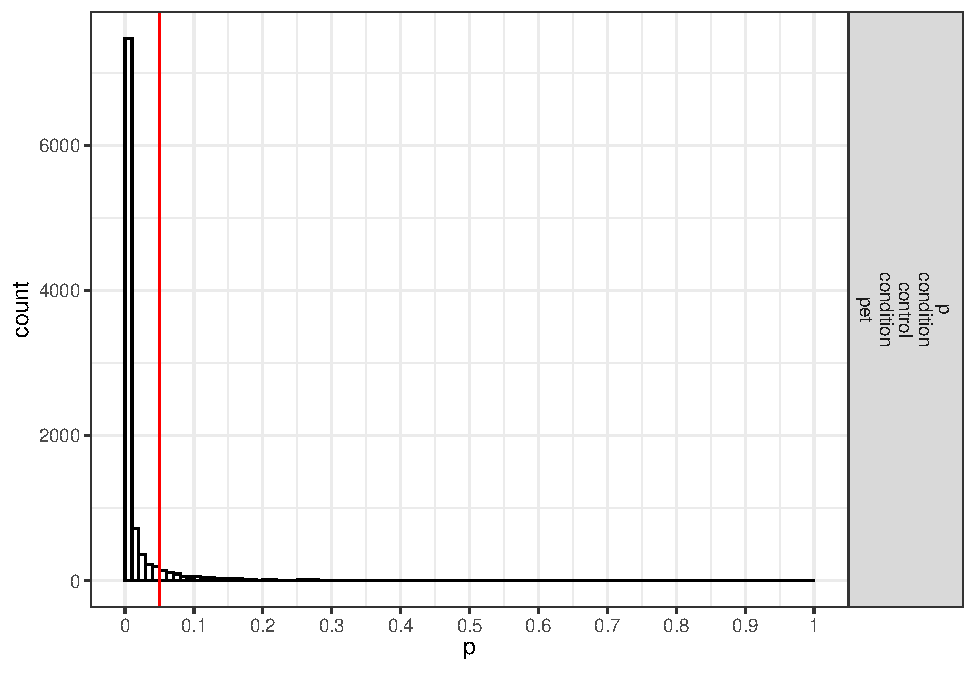
\includegraphics{SuperpowerValidation_files/figure-latex/unnamed-chunk-25-1.pdf}

\begin{Shaded}
\begin{Highlighting}[]
\KeywordTok{ANOVA_power}\NormalTok{(design_result, }\DataTypeTok{nsims =}\NormalTok{ nsims)}
\end{Highlighting}
\end{Shaded}

\begin{verbatim}
## Power and Effect sizes for ANOVA tests
##               power effect_size
## anova_factor1    82     0.04214
## 
## Power and Effect sizes for contrasts
##                                 power effect_size
## p_factor1_level1_factor1_level2    74    0.401812
## p_factor1_level1_factor1_level3    72    0.398766
## p_factor1_level2_factor1_level3     7   -0.002054
\end{verbatim}

\hypertarget{variation-1}{%
\section{Variation 1}\label{variation-1}}

\begin{Shaded}
\begin{Highlighting}[]
\CommentTok{# give sample sizes (all samples sizes are equal)}
\NormalTok{N =}\StringTok{ }\DecValTok{145}
\CommentTok{# give effect size d}
\NormalTok{d1 =}\StringTok{ }\FloatTok{.4} \CommentTok{#difference between the extremes}
\NormalTok{d2 =}\StringTok{ }\FloatTok{.0} \CommentTok{#third condition goes with the highest extreme}
\CommentTok{# give number of simulations}
\NormalTok{nSim =}\StringTok{ }\NormalTok{nsims}
\CommentTok{# give alpha levels}
\NormalTok{alpha1 =}\StringTok{ }\FloatTok{.05} \CommentTok{#alpha level for the omnibus ANOVA}
\NormalTok{alpha2 =}\StringTok{ }\FloatTok{.05} \CommentTok{#alpha level for three post hoc one-tailed t-tests Bonferroni correction}
\CommentTok{# create progress bar in case it takes a while}
\CommentTok{#pb <- winProgressBar(title = "progress bar", min = 0, max = nSim, width = 300)}
\CommentTok{# create vectors to store p-values}
\NormalTok{p1 <-}\KeywordTok{numeric}\NormalTok{(nSim) }\CommentTok{#p-value omnibus ANOVA}
\NormalTok{p2 <-}\KeywordTok{numeric}\NormalTok{(nSim) }\CommentTok{#p-value first post hoc test}
\NormalTok{p3 <-}\KeywordTok{numeric}\NormalTok{(nSim) }\CommentTok{#p-value second post hoc test}
\NormalTok{p4 <-}\KeywordTok{numeric}\NormalTok{(nSim) }\CommentTok{#p-value third post hoc test}
\NormalTok{pes1 <-}\KeywordTok{numeric}\NormalTok{(nSim) }\CommentTok{#partial eta-squared}
\NormalTok{pes2 <-}\KeywordTok{numeric}\NormalTok{(nSim) }\CommentTok{#partial eta-squared two extreme conditions}
\KeywordTok{library}\NormalTok{(lsr)}
\ControlFlowTok{for}\NormalTok{(i }\ControlFlowTok{in} \DecValTok{1}\OperatorTok{:}\NormalTok{nSim)\{ }\CommentTok{#for each simulated experiment}
 \CommentTok{# setWinProgressBar(pb, i, title=paste(round(i/nSim*100, 1), "% done"))}
\NormalTok{  x<-}\KeywordTok{rnorm}\NormalTok{(}\DataTypeTok{n =}\NormalTok{ N, }\DataTypeTok{mean =} \DecValTok{0}\NormalTok{, }\DataTypeTok{sd =} \DecValTok{1}\NormalTok{)}
\NormalTok{  y<-}\KeywordTok{rnorm}\NormalTok{(}\DataTypeTok{n =}\NormalTok{ N, }\DataTypeTok{mean =}\NormalTok{ d1, }\DataTypeTok{sd =} \DecValTok{1}\NormalTok{) }
\NormalTok{  z<-}\KeywordTok{rnorm}\NormalTok{(}\DataTypeTok{n =}\NormalTok{ N, }\DataTypeTok{mean =}\NormalTok{ d2, }\DataTypeTok{sd =} \DecValTok{1}\NormalTok{) }
\NormalTok{  data =}\StringTok{ }\KeywordTok{c}\NormalTok{(x,y,z)}
\NormalTok{  groups=}\StringTok{ }\KeywordTok{factor}\NormalTok{(}\KeywordTok{rep}\NormalTok{(letters[}\DecValTok{24}\OperatorTok{:}\DecValTok{26}\NormalTok{], }\DataTypeTok{each =}\NormalTok{ N))}
\NormalTok{  test <-}\StringTok{ }\KeywordTok{aov}\NormalTok{(data}\OperatorTok{~}\NormalTok{groups)}
\NormalTok{  pes1[i] <-}\StringTok{ }\KeywordTok{etaSquared}\NormalTok{(test)[}\DecValTok{1}\NormalTok{,}\DecValTok{2}\NormalTok{]}
\NormalTok{  p1[i] <-}\StringTok{ }\KeywordTok{summary}\NormalTok{(test)[[}\DecValTok{1}\NormalTok{]][[}\StringTok{"Pr(>F)"}\NormalTok{]][[}\DecValTok{1}\NormalTok{]]}
\NormalTok{  p2[i] <-}\StringTok{ }\KeywordTok{t.test}\NormalTok{(x,y)}\OperatorTok{$}\NormalTok{p.value}
\NormalTok{  p3[i] <-}\StringTok{ }\KeywordTok{t.test}\NormalTok{(x,z)}\OperatorTok{$}\NormalTok{p.value}
\NormalTok{  p4[i] <-}\StringTok{ }\KeywordTok{t.test}\NormalTok{(y,z)}\OperatorTok{$}\NormalTok{p.value}
\NormalTok{  data =}\StringTok{ }\KeywordTok{c}\NormalTok{(x,y)}
\NormalTok{  groups=}\StringTok{ }\KeywordTok{factor}\NormalTok{(}\KeywordTok{rep}\NormalTok{(letters[}\DecValTok{24}\OperatorTok{:}\DecValTok{25}\NormalTok{], }\DataTypeTok{each =}\NormalTok{ N))}
\NormalTok{  test <-}\StringTok{ }\KeywordTok{aov}\NormalTok{(data}\OperatorTok{~}\NormalTok{groups)}
\NormalTok{  pes2[i] <-}\StringTok{ }\KeywordTok{etaSquared}\NormalTok{(test)[}\DecValTok{1}\NormalTok{,}\DecValTok{2}\NormalTok{]}
\NormalTok{  \}}
\CommentTok{#close(pb)#close progress bar}
\CommentTok{# results are as predicted when omnibus ANOVA is significant, t-tests are significant between x and y plus x and z; not significant between y and z}
\CommentTok{#printing all unique tests (adjusted code by DL)}
\KeywordTok{sum}\NormalTok{(p1}\OperatorTok{<}\NormalTok{alpha1)}\OperatorTok{/}\NormalTok{nSim}
\end{Highlighting}
\end{Shaded}

\begin{verbatim}
## [1] 0.94
\end{verbatim}

\begin{Shaded}
\begin{Highlighting}[]
\KeywordTok{sum}\NormalTok{(p2}\OperatorTok{<}\NormalTok{alpha2)}\OperatorTok{/}\NormalTok{nSim}
\end{Highlighting}
\end{Shaded}

\begin{verbatim}
## [1] 0.89
\end{verbatim}

\begin{Shaded}
\begin{Highlighting}[]
\KeywordTok{sum}\NormalTok{(p3}\OperatorTok{<}\NormalTok{alpha2)}\OperatorTok{/}\NormalTok{nSim}
\end{Highlighting}
\end{Shaded}

\begin{verbatim}
## [1] 0.05
\end{verbatim}

\begin{Shaded}
\begin{Highlighting}[]
\KeywordTok{sum}\NormalTok{(p4}\OperatorTok{<}\NormalTok{alpha2)}\OperatorTok{/}\NormalTok{nSim}
\end{Highlighting}
\end{Shaded}

\begin{verbatim}
## [1] 0.94
\end{verbatim}

\begin{Shaded}
\begin{Highlighting}[]
\KeywordTok{mean}\NormalTok{(pes1)}
\end{Highlighting}
\end{Shaded}

\begin{verbatim}
## [1] 0.04057115
\end{verbatim}

\begin{Shaded}
\begin{Highlighting}[]
\KeywordTok{mean}\NormalTok{(pes2)}
\end{Highlighting}
\end{Shaded}

\begin{verbatim}
## [1] 0.04531236
\end{verbatim}

\hypertarget{three-conditions-replication-1}{%
\section{Three conditions replication}\label{three-conditions-replication-1}}

\begin{Shaded}
\begin{Highlighting}[]
\NormalTok{K <-}\StringTok{ }\DecValTok{3}
\NormalTok{mu <-}\StringTok{ }\KeywordTok{c}\NormalTok{(}\DecValTok{0}\NormalTok{, }\FloatTok{0.4}\NormalTok{, }\FloatTok{0.0}\NormalTok{)}
\NormalTok{n <-}\StringTok{ }\DecValTok{145}
\NormalTok{sd <-}\StringTok{ }\DecValTok{1}
\NormalTok{r <-}\StringTok{ }\DecValTok{0}
\NormalTok{design =}\KeywordTok{paste}\NormalTok{(K,}\StringTok{"b"}\NormalTok{,}\DataTypeTok{sep=}\StringTok{""}\NormalTok{)}
\end{Highlighting}
\end{Shaded}

\begin{Shaded}
\begin{Highlighting}[]
\NormalTok{design_result <-}\StringTok{ }\KeywordTok{ANOVA_design}\NormalTok{(}\DataTypeTok{design =}\NormalTok{string,}
                   \DataTypeTok{n =}\NormalTok{ n, }
                   \DataTypeTok{mu =}\NormalTok{ mu, }
                   \DataTypeTok{sd =}\NormalTok{ sd, }
                   \DataTypeTok{labelnames =} \KeywordTok{c}\NormalTok{(}\StringTok{"factor1"}\NormalTok{, }\StringTok{"level1"}\NormalTok{, }\StringTok{"level2"}\NormalTok{, }\StringTok{"level3"}\NormalTok{))}
\end{Highlighting}
\end{Shaded}

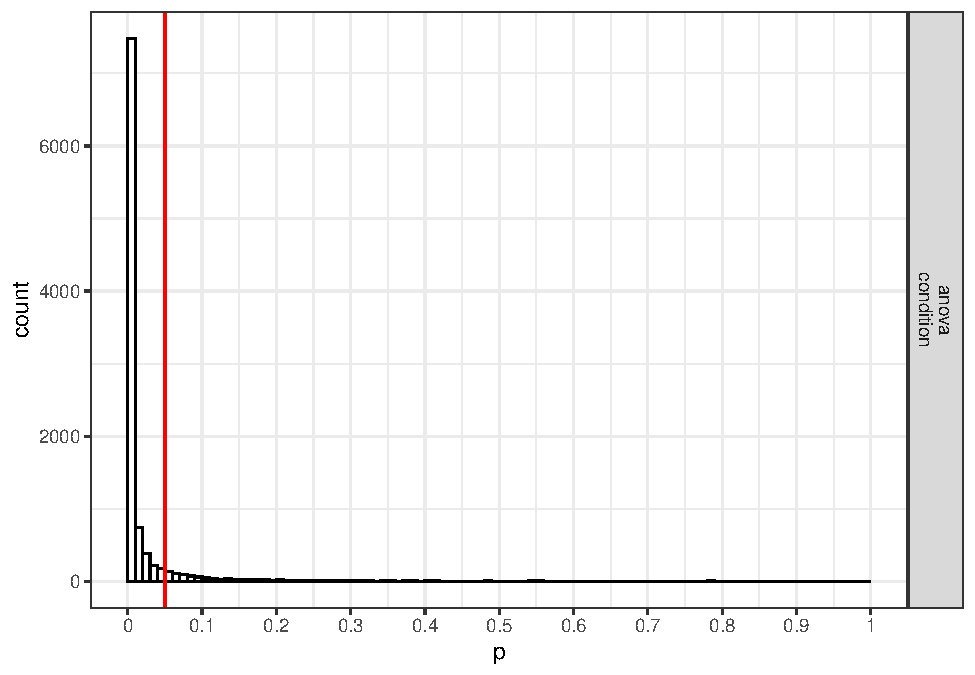
\includegraphics{SuperpowerValidation_files/figure-latex/unnamed-chunk-28-1.pdf}

\begin{Shaded}
\begin{Highlighting}[]
\KeywordTok{ANOVA_power}\NormalTok{(design_result, }\DataTypeTok{nsims =}\NormalTok{ nsims)}
\end{Highlighting}
\end{Shaded}

\begin{verbatim}
## Power and Effect sizes for ANOVA tests
##               power effect_size
## anova_factor1    92     0.03798
## 
## Power and Effect sizes for contrasts
##                                 power effect_size
## p_factor1_level1_factor1_level2    93    0.394404
## p_factor1_level1_factor1_level3     6    0.005287
## p_factor1_level2_factor1_level3    88   -0.391447
\end{verbatim}

\hypertarget{variation-2}{%
\section{Variation 2}\label{variation-2}}

\begin{Shaded}
\begin{Highlighting}[]
\CommentTok{# give sample sizes (all samples sizes are equal)}
\NormalTok{N =}\StringTok{ }\DecValTok{82}
\CommentTok{# give effect size d}
\NormalTok{d1 =}\StringTok{ }\FloatTok{.4} \CommentTok{#difference between the extremes}
\NormalTok{d2 =}\StringTok{ }\FloatTok{.2} \CommentTok{#third condition goes with the highest extreme}
\CommentTok{# give number of simulations}
\NormalTok{nSim =}\StringTok{ }\NormalTok{nsims}
\CommentTok{# give alpha levels}
\NormalTok{alpha1 =}\StringTok{ }\FloatTok{.05} \CommentTok{#alpha level for the omnibus ANOVA}
\NormalTok{alpha2 =}\StringTok{ }\FloatTok{.05} \CommentTok{#alpha level for three post hoc one-tailed t-tests Bonferroni correction}
\CommentTok{# create progress bar in case it takes a while}
\CommentTok{#pb <- winProgressBar(title = "progress bar", min = 0, max = nSim, width = 300)}
\CommentTok{# create vectors to store p-values}
\NormalTok{p1 <-}\KeywordTok{numeric}\NormalTok{(nSim) }\CommentTok{#p-value omnibus ANOVA}
\NormalTok{p2 <-}\KeywordTok{numeric}\NormalTok{(nSim) }\CommentTok{#p-value first post hoc test}
\NormalTok{p3 <-}\KeywordTok{numeric}\NormalTok{(nSim) }\CommentTok{#p-value second post hoc test}
\NormalTok{p4 <-}\KeywordTok{numeric}\NormalTok{(nSim) }\CommentTok{#p-value third post hoc test}
\NormalTok{pes1 <-}\KeywordTok{numeric}\NormalTok{(nSim) }\CommentTok{#partial eta-squared}
\NormalTok{pes2 <-}\KeywordTok{numeric}\NormalTok{(nSim) }\CommentTok{#partial eta-squared two extreme conditions}
\KeywordTok{library}\NormalTok{(lsr)}
\ControlFlowTok{for}\NormalTok{(i }\ControlFlowTok{in} \DecValTok{1}\OperatorTok{:}\NormalTok{nSim)\{ }\CommentTok{#for each simulated experiment}
 \CommentTok{# setWinProgressBar(pb, i, title=paste(round(i/nSim*100, 1), "% done"))}
\NormalTok{  x<-}\KeywordTok{rnorm}\NormalTok{(}\DataTypeTok{n =}\NormalTok{ N, }\DataTypeTok{mean =} \DecValTok{0}\NormalTok{, }\DataTypeTok{sd =} \DecValTok{1}\NormalTok{)}
\NormalTok{  y<-}\KeywordTok{rnorm}\NormalTok{(}\DataTypeTok{n =}\NormalTok{ N, }\DataTypeTok{mean =}\NormalTok{ d1, }\DataTypeTok{sd =} \DecValTok{1}\NormalTok{) }
\NormalTok{  z<-}\KeywordTok{rnorm}\NormalTok{(}\DataTypeTok{n =}\NormalTok{ N, }\DataTypeTok{mean =}\NormalTok{ d2, }\DataTypeTok{sd =} \DecValTok{1}\NormalTok{) }
\NormalTok{  data =}\StringTok{ }\KeywordTok{c}\NormalTok{(x,y,z)}
\NormalTok{  groups=}\StringTok{ }\KeywordTok{factor}\NormalTok{(}\KeywordTok{rep}\NormalTok{(letters[}\DecValTok{24}\OperatorTok{:}\DecValTok{26}\NormalTok{], }\DataTypeTok{each =}\NormalTok{ N))}
\NormalTok{  test <-}\StringTok{ }\KeywordTok{aov}\NormalTok{(data}\OperatorTok{~}\NormalTok{groups)}
\NormalTok{  pes1[i] <-}\StringTok{ }\KeywordTok{etaSquared}\NormalTok{(test)[}\DecValTok{1}\NormalTok{,}\DecValTok{2}\NormalTok{]}
\NormalTok{  p1[i] <-}\StringTok{ }\KeywordTok{summary}\NormalTok{(test)[[}\DecValTok{1}\NormalTok{]][[}\StringTok{"Pr(>F)"}\NormalTok{]][[}\DecValTok{1}\NormalTok{]]}
\NormalTok{  p2[i] <-}\StringTok{ }\KeywordTok{t.test}\NormalTok{(x,y)}\OperatorTok{$}\NormalTok{p.value}
\NormalTok{  p3[i] <-}\StringTok{ }\KeywordTok{t.test}\NormalTok{(x,z)}\OperatorTok{$}\NormalTok{p.value}
\NormalTok{  p4[i] <-}\StringTok{ }\KeywordTok{t.test}\NormalTok{(y,z)}\OperatorTok{$}\NormalTok{p.value}
\NormalTok{  data =}\StringTok{ }\KeywordTok{c}\NormalTok{(x,y)}
\NormalTok{  groups=}\StringTok{ }\KeywordTok{factor}\NormalTok{(}\KeywordTok{rep}\NormalTok{(letters[}\DecValTok{24}\OperatorTok{:}\DecValTok{25}\NormalTok{], }\DataTypeTok{each =}\NormalTok{ N))}
\NormalTok{  test <-}\StringTok{ }\KeywordTok{aov}\NormalTok{(data}\OperatorTok{~}\NormalTok{groups)}
\NormalTok{  pes2[i] <-}\StringTok{ }\KeywordTok{etaSquared}\NormalTok{(test)[}\DecValTok{1}\NormalTok{,}\DecValTok{2}\NormalTok{]}
\NormalTok{  \}}
\CommentTok{#close(pb)#close progress bar}
\CommentTok{# results are as predicted when omnibus ANOVA is significant, t-tests are significant between x and y plus x and z; not significant between y and z}
\CommentTok{#printing all unique tests (adjusted code by DL)}
\KeywordTok{sum}\NormalTok{(p1}\OperatorTok{<}\NormalTok{alpha1)}\OperatorTok{/}\NormalTok{nSim}
\end{Highlighting}
\end{Shaded}

\begin{verbatim}
## [1] 0.63
\end{verbatim}

\begin{Shaded}
\begin{Highlighting}[]
\KeywordTok{sum}\NormalTok{(p2}\OperatorTok{<}\NormalTok{alpha2)}\OperatorTok{/}\NormalTok{nSim}
\end{Highlighting}
\end{Shaded}

\begin{verbatim}
## [1] 0.73
\end{verbatim}

\begin{Shaded}
\begin{Highlighting}[]
\KeywordTok{sum}\NormalTok{(p3}\OperatorTok{<}\NormalTok{alpha2)}\OperatorTok{/}\NormalTok{nSim}
\end{Highlighting}
\end{Shaded}

\begin{verbatim}
## [1] 0.18
\end{verbatim}

\begin{Shaded}
\begin{Highlighting}[]
\KeywordTok{sum}\NormalTok{(p4}\OperatorTok{<}\NormalTok{alpha2)}\OperatorTok{/}\NormalTok{nSim}
\end{Highlighting}
\end{Shaded}

\begin{verbatim}
## [1] 0.3
\end{verbatim}

\begin{Shaded}
\begin{Highlighting}[]
\KeywordTok{mean}\NormalTok{(pes1)}
\end{Highlighting}
\end{Shaded}

\begin{verbatim}
## [1] 0.03383246
\end{verbatim}

\begin{Shaded}
\begin{Highlighting}[]
\KeywordTok{mean}\NormalTok{(pes2)}
\end{Highlighting}
\end{Shaded}

\begin{verbatim}
## [1] 0.0425566
\end{verbatim}

\hypertarget{three-conditions-replication-2}{%
\section{Three conditions replication}\label{three-conditions-replication-2}}

\begin{Shaded}
\begin{Highlighting}[]
\NormalTok{K <-}\StringTok{ }\DecValTok{3}
\NormalTok{mu <-}\StringTok{ }\KeywordTok{c}\NormalTok{(}\DecValTok{0}\NormalTok{, }\FloatTok{0.4}\NormalTok{, }\FloatTok{0.2}\NormalTok{)}
\NormalTok{n <-}\StringTok{ }\DecValTok{82}
\NormalTok{sd <-}\StringTok{ }\DecValTok{1}
\NormalTok{design =}\KeywordTok{paste}\NormalTok{(K,}\StringTok{"b"}\NormalTok{,}\DataTypeTok{sep=}\StringTok{""}\NormalTok{)}
\end{Highlighting}
\end{Shaded}

\begin{Shaded}
\begin{Highlighting}[]
\NormalTok{design_result <-}\StringTok{ }\KeywordTok{ANOVA_design}\NormalTok{(}\DataTypeTok{design =}\NormalTok{string,}
                   \DataTypeTok{n =}\NormalTok{ n, }
                   \DataTypeTok{mu =}\NormalTok{ mu, }
                   \DataTypeTok{sd =}\NormalTok{ sd, }
                   \DataTypeTok{labelnames =} \KeywordTok{c}\NormalTok{(}\StringTok{"factor1"}\NormalTok{, }\StringTok{"level1"}\NormalTok{, }\StringTok{"level2"}\NormalTok{, }\StringTok{"level3"}\NormalTok{))}
\end{Highlighting}
\end{Shaded}

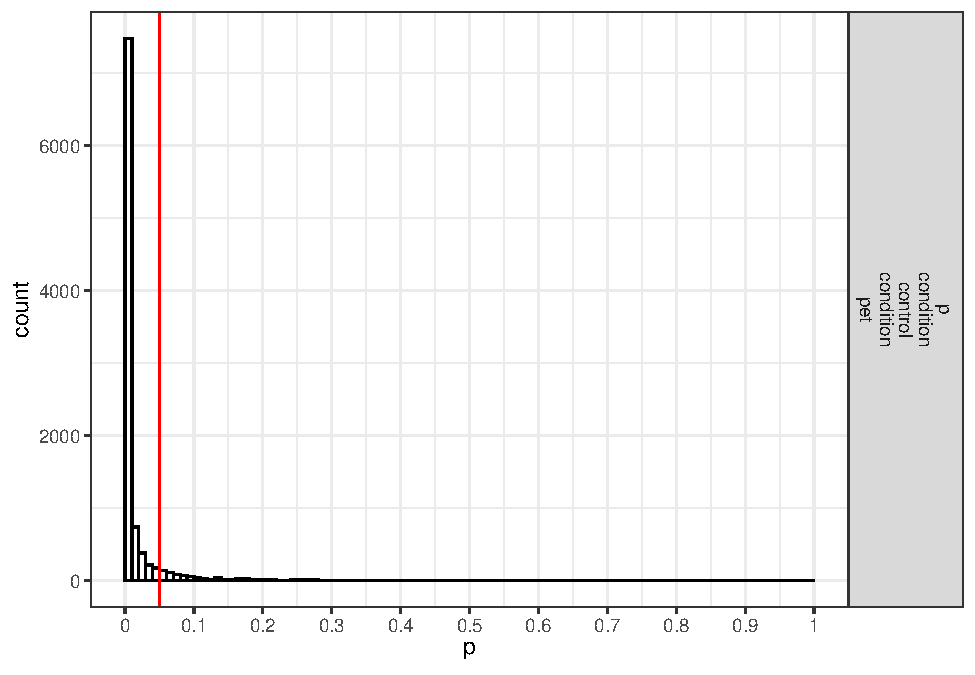
\includegraphics{SuperpowerValidation_files/figure-latex/unnamed-chunk-31-1.pdf}

\begin{Shaded}
\begin{Highlighting}[]
\KeywordTok{ANOVA_power}\NormalTok{(design_result, }\DataTypeTok{nsims =}\NormalTok{ nsims)}
\end{Highlighting}
\end{Shaded}

\begin{verbatim}
## Power and Effect sizes for ANOVA tests
##               power effect_size
## anova_factor1    64      0.0368
## 
## Power and Effect sizes for contrasts
##                                 power effect_size
## p_factor1_level1_factor1_level2    77      0.4242
## p_factor1_level1_factor1_level3    21      0.2039
## p_factor1_level2_factor1_level3    26     -0.2198
\end{verbatim}

\hypertarget{repeated-measures-anova-part-1}{%
\chapter{Repeated Measures-ANOVA Part 1}\label{repeated-measures-anova-part-1}}

In a repeated measures design multiple observations are collected from the same participants. In the simplest case, where there are two repeated observations, a repeated measures ANOVA equals a dependent or paired \emph{t}-test. The difference compared to a between subject design is that repeated measures can be correlated, and in psychology, they often are. Let's first explore the impact of this correlation on the power of a repeated measures ANOVA.

\hypertarget{two-conditions-medium-effect-size}{%
\section{Two conditions, medium effect size}\label{two-conditions-medium-effect-size}}

To illustrate the effect of correated observations, we start by simulating data for a medium effect size for a dependent (or paired, or within-subject) \emph{t}-test. Let's first look at G*power. If we want to perform an a-priori power analysis, we are asked to fill in the effect size dz. As Cohen (1988) writes, ``The Z subscript is used to emphasize the fact that our raw score unit is no longer X or Y, but Z'', where Z are the difference scores of X-Y.

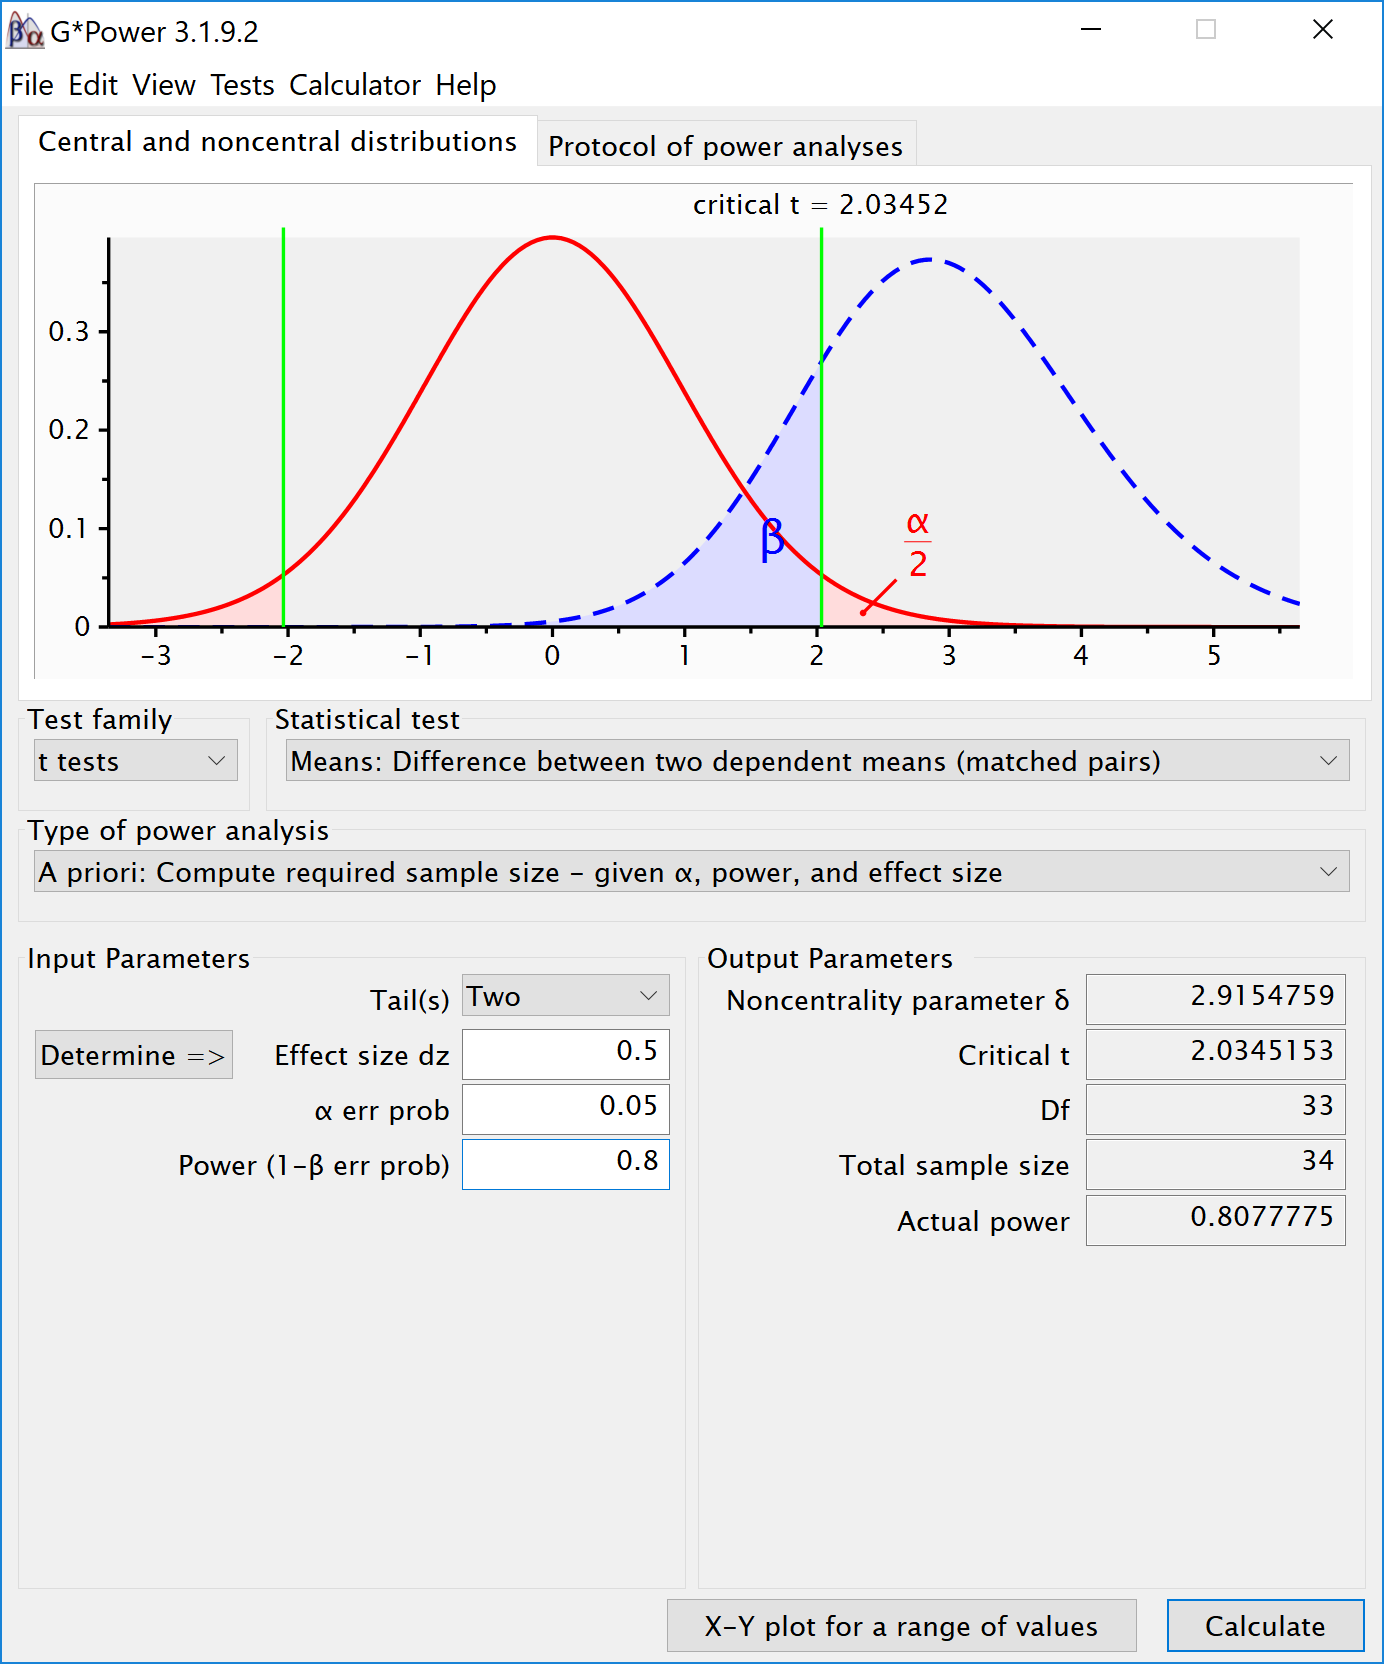
\includegraphics{screenshots/gpower_9.png}

Within designs can have greater power to detect differences than between designs because the values are correlated, and a within design requires less participants because each participant provides multiple observations. One difference between an independent \emph{t}-test and a dependent \emph{t}-test is that an independent \emph{t}-test has 2(n-1) degrees of freedom, while a dependent \emph{t}-test has (n-1) degrees of freedom. The sample size needed in a two-group within-design (NW) relative to the sample needed in two-group between-designs (NB), assuming normal distributions, and ignoring the difference in degrees of freedom between the two types of tests, is (from Maxwell \& Delaney, 2004, p.~561, formula 45):

\(N_{W}=\frac{N_{B}(1-\rho)}{2}\)

The division by 2 in the equation is due to the fact that in a two-condition within design every participant provides two data-points. The extent to which this reduces the sample size compared to a between-subject design depends on the correlation (\emph{r}) between the two dependent variables, as indicated by the 1-r part of the equation. If the correlation is 0, a within-subject design needs half as many participants as a between-subject design (e.g., 64 instead 128 participants), simply because every participants provides 2 datapoints. The higher the correlation, the larger the relative benefit of within designs, and whenever the correlation is negative (up to -1) the relative benefit disappears.

Whereas in an independent \emph{t}-test the two observations are uncorrelated, in a within design the observations are correlated. This has an effect on the standard deviation of the difference scores. In turn, because the standardized effect size is the mean difference divided by the standard deviation of the difference scores, the correlation has an effect on the standardized mean difference in a within design, Cohen's dz. The relation, as Cohen (1988, formula 2.3.7) explains, is:

\(\sigma_{z}=\sigma\sqrt{2(1-\rho)}\)

Therefore, the relation between dz and d is \(\sqrt{2(1-\rho)}\). As Cohen (1988) writes: "In other words, a given difference between population means for matched (dependent) samples is standardized by a value which is \(\sqrt{2(1-\rho)}\) as large as would be the case were they independent. If we enter a correlation of 0.5 in the formula, we get \(\sqrt{2(0.5)}=1\). In other words, when the correlation is 0.5, d = dz. When there is a strong correlation between dependent variables, for example r = 0.9, we get \(d=d_{z}\sqrt{2(1-0.9)}\), and a dz of 1 would be a d = 0.45. Reversely, \(d_{z}=\frac{d}{\sqrt{2(1-r)}}\), so with a r = 0.9, a d of 1 would be a dz = 2.24. Some consider this increase in dz compared to d when observations are strongly correlated an `inflation' when estimating effect sizes, but since the reduction in the standard deviation of the difference scores due to the correlation makes it easier to distinguish signal from noise in a hypothesis test, it leads to a clear power benefit.

\begin{Shaded}
\begin{Highlighting}[]
\CommentTok{# Check sample size formula Maxwell}
\CommentTok{# Power is pretty similar with n/2, same d (assuming r = 0.5). }
\CommentTok{# Small differences due to df = 2(n-1) vs df = n-1}
\KeywordTok{pwr.t.test}\NormalTok{(}\DataTypeTok{d =} \FloatTok{0.05}\NormalTok{,}
           \DataTypeTok{n =} \KeywordTok{c}\NormalTok{(}\DecValTok{2000}\NormalTok{, }\DecValTok{4000}\NormalTok{, }\DecValTok{8000}\NormalTok{),}
           \DataTypeTok{sig.level =} \FloatTok{0.05}\NormalTok{,}
           \DataTypeTok{type =} \StringTok{"two.sample"}\NormalTok{,}
           \DataTypeTok{alternative =} \StringTok{"two.sided"}\NormalTok{)}
\end{Highlighting}
\end{Shaded}

\begin{verbatim}
## 
##      Two-sample t test power calculation 
## 
##               n = 2000, 4000, 8000
##               d = 0.05
##       sig.level = 0.05
##           power = 0.3524674, 0.6086764, 0.8853424
##     alternative = two.sided
## 
## NOTE: n is number in *each* group
\end{verbatim}

\begin{Shaded}
\begin{Highlighting}[]
\KeywordTok{pwr.t.test}\NormalTok{(}\DataTypeTok{d =} \FloatTok{0.05}\NormalTok{,}
           \DataTypeTok{n =} \KeywordTok{c}\NormalTok{(}\DecValTok{1000}\NormalTok{, }\DecValTok{2000}\NormalTok{, }\DecValTok{4000}\NormalTok{),}
           \DataTypeTok{sig.level =} \FloatTok{0.05}\NormalTok{,}
           \DataTypeTok{type =} \StringTok{"paired"}\NormalTok{,}
           \DataTypeTok{alternative =} \StringTok{"two.sided"}\NormalTok{)}
\end{Highlighting}
\end{Shaded}

\begin{verbatim}
## 
##      Paired t test power calculation 
## 
##               n = 1000, 2000, 4000
##               d = 0.05
##       sig.level = 0.05
##           power = 0.3520450, 0.6083669, 0.8852320
##     alternative = two.sided
## 
## NOTE: n is number of *pairs*
\end{verbatim}

There is no equivalent fz for Cohen's f for a within subject ANOVA. For two groups, we can directly compute Cohen's f from Cohen's d for two groups, as Cohen (1988) describes, because f = 1/2d. For a d = 0.5, f = 0.25. In Gpower we can run a 2 group within-subject power analysis for ANOVA. We plan for 80\% power, and reproduce the anaysis above for the dependent \emph{t}-test. This works because the correlation is set to 0.5, when d = dz, and thus the transformation of f=1/2d works.

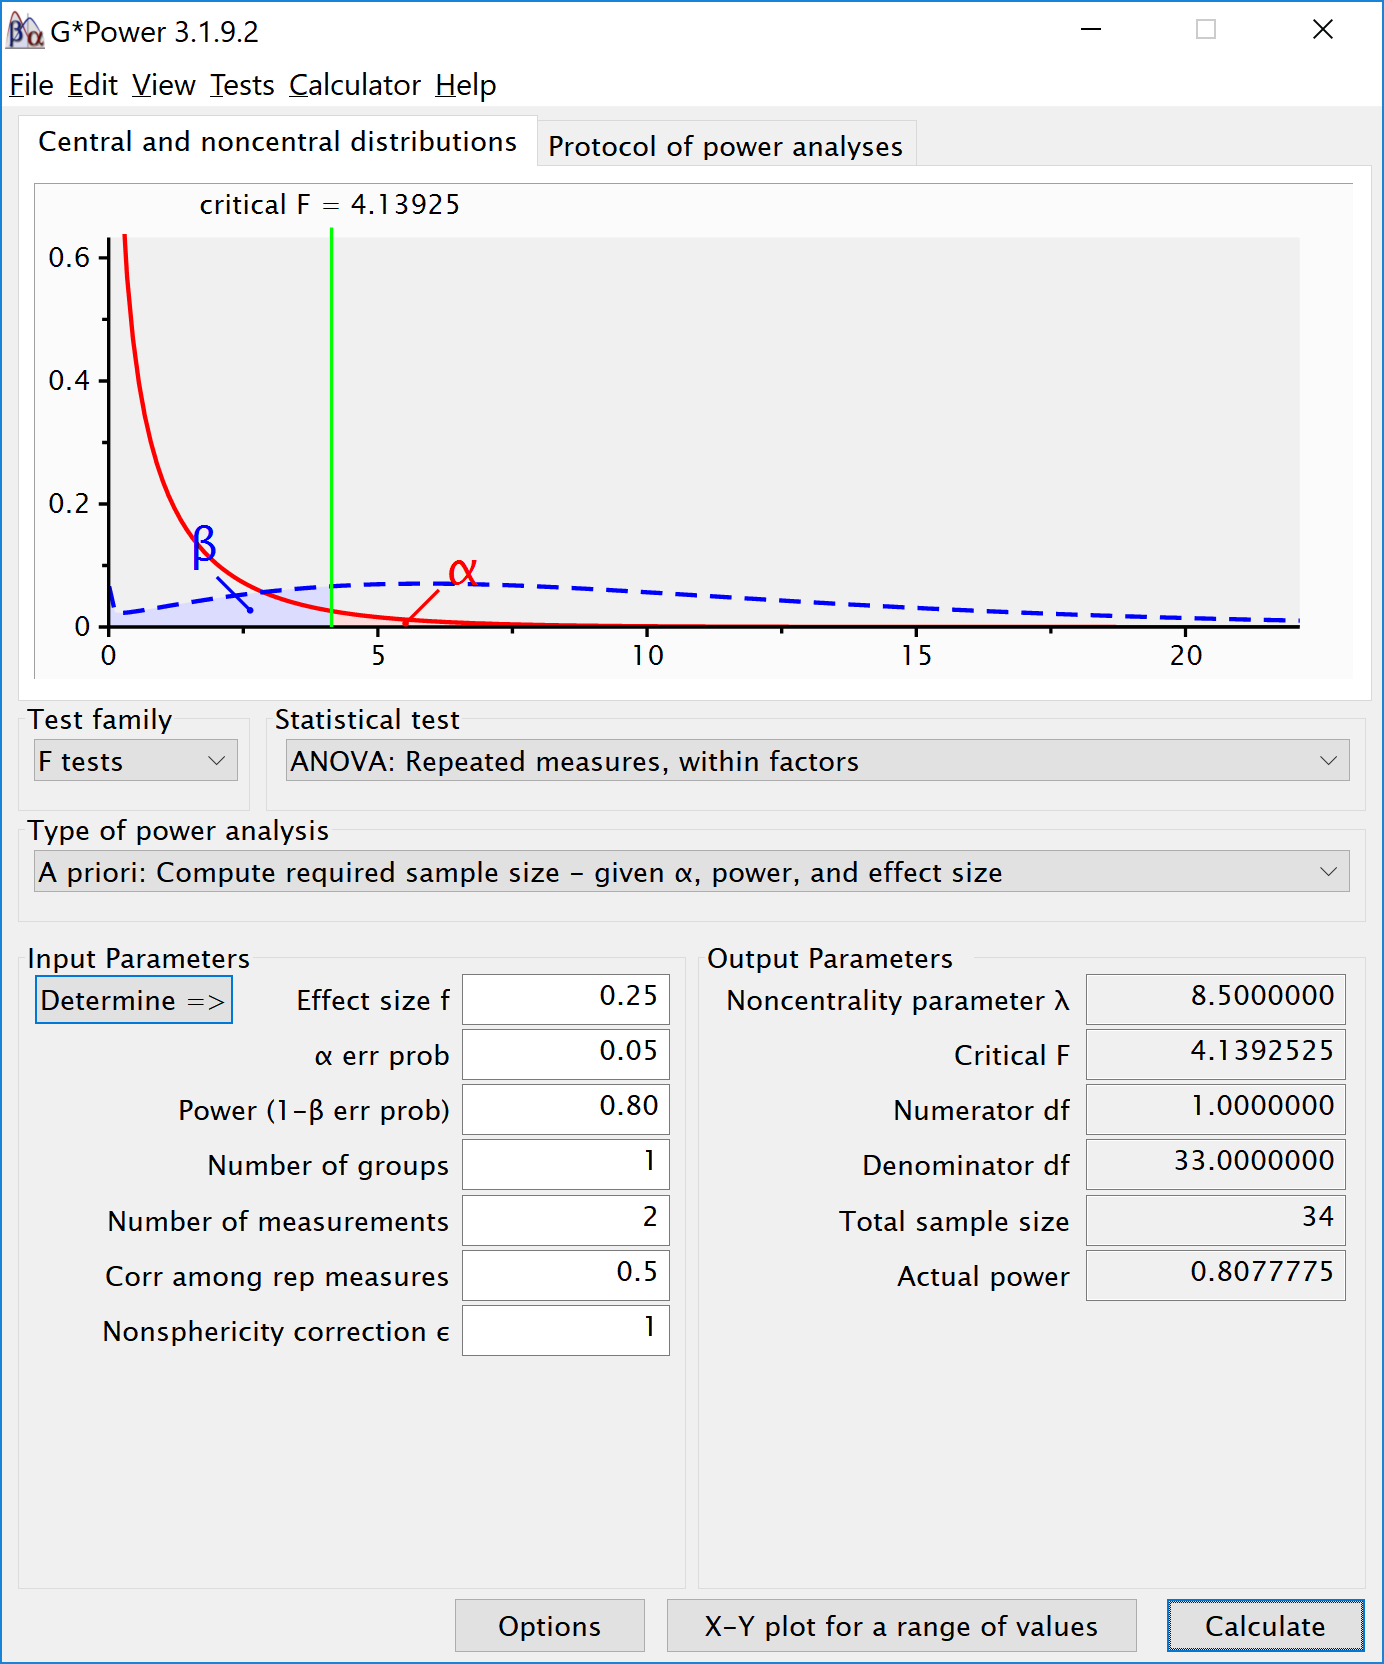
\includegraphics{screenshots/gpower_1.png}

If we change the correlation to 0.7 and keep all other settings the same, the repeated measure a-priori power analysis yields a sample of 21. The correlation increases the power for the test.

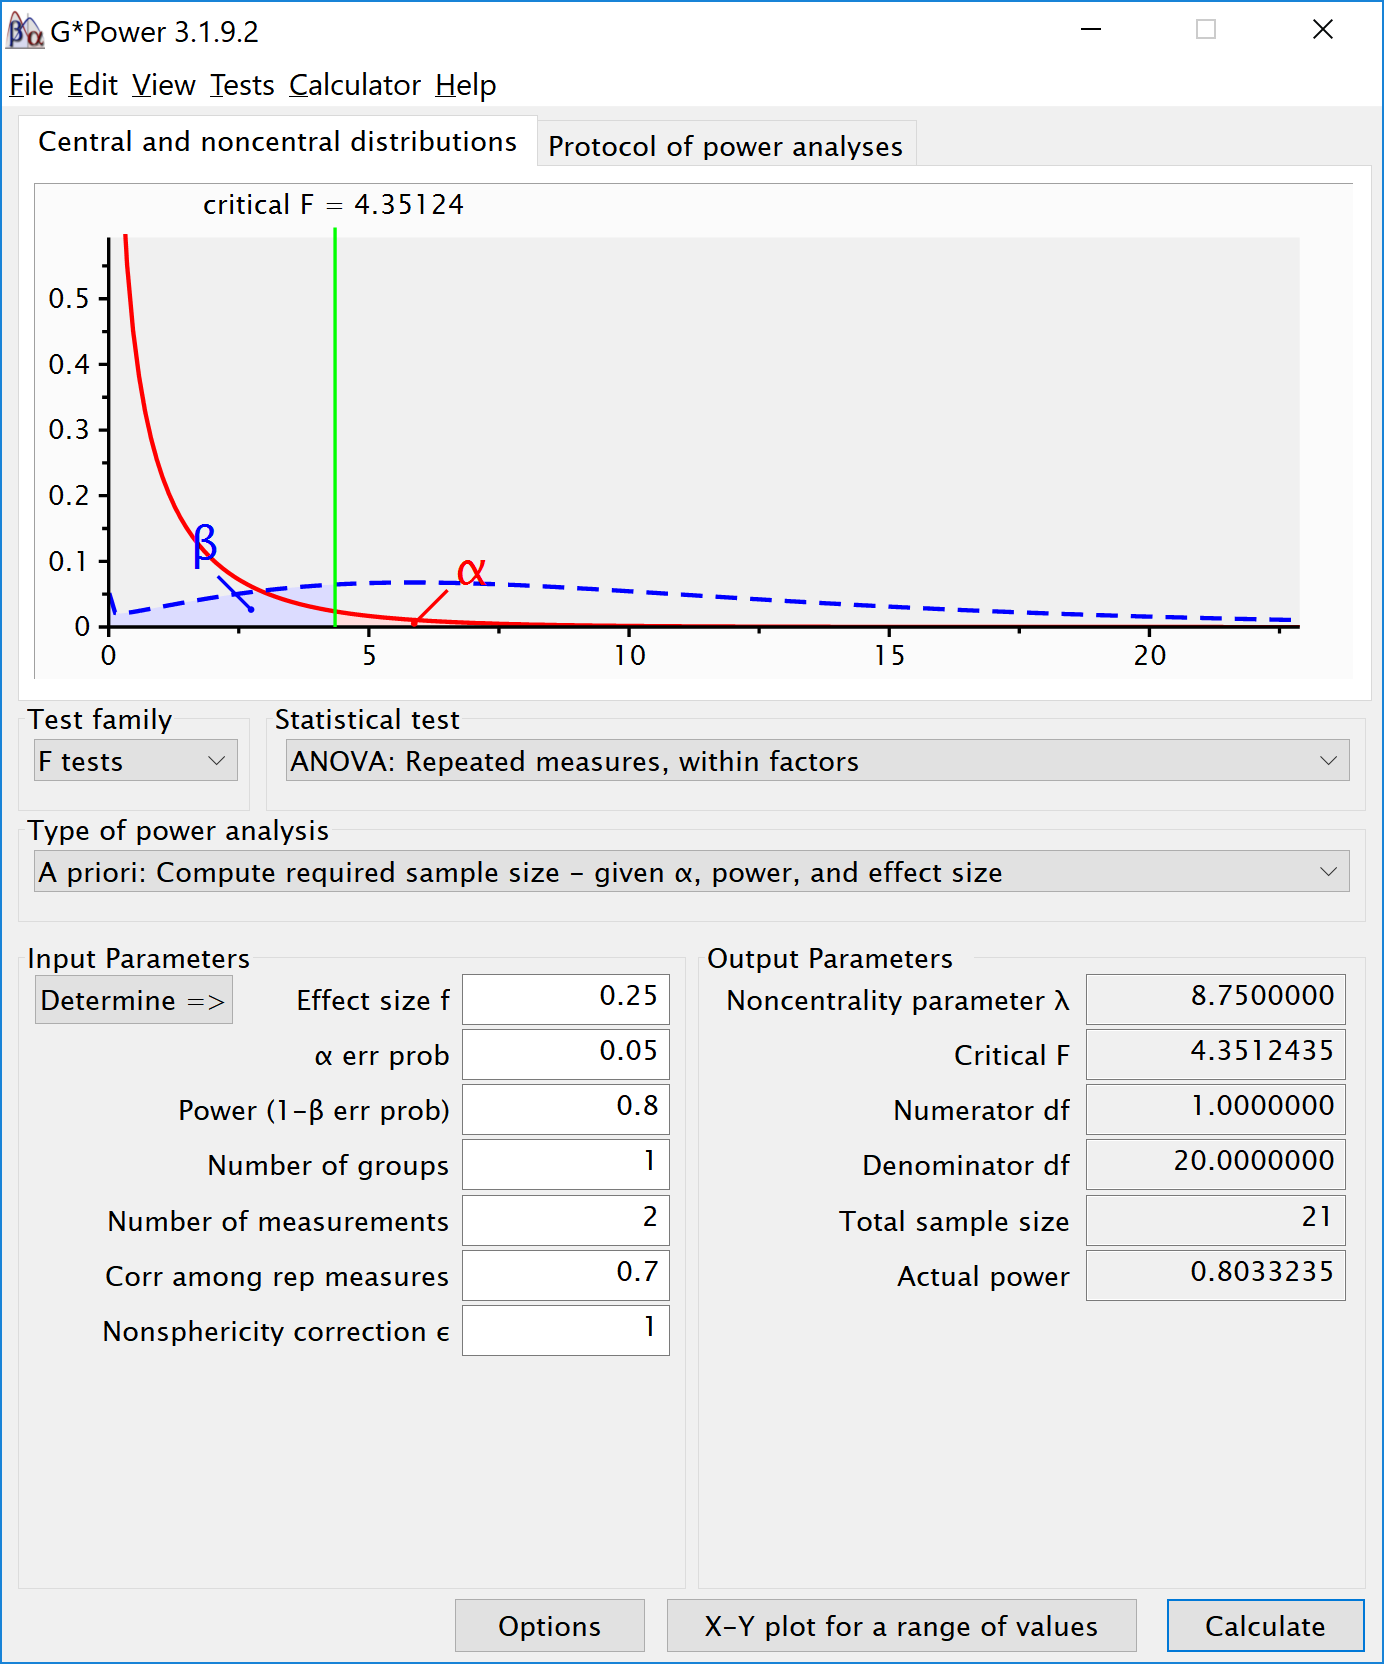
\includegraphics{screenshots/gpower_11.png}

To reproduce this analysis in Gpower with a dependent \emph{t}-test we need to change dz following the formula above, \(d_{z}=\frac{0.5}{\sqrt{2(1-0.7)}}\), which yields dz = 0.6454972. If we enter this value in Gpower for an a-priori power analysis, we get the exact same results (as we should, since an repeated measures ANOVA with 2 groups equals a dependent \emph{t}-test). This example illustrates that the correlation between dependent variables always factors into a power analysis, both for a dependent \emph{t}-test, and for a repeated measures ANOVA. Because a dependent \emph{t}-test uses dz the correlation might be less visible, but given the relation between d and dz, the correlation is always taken into account and can greatly improve power for within designs compared to between designs.

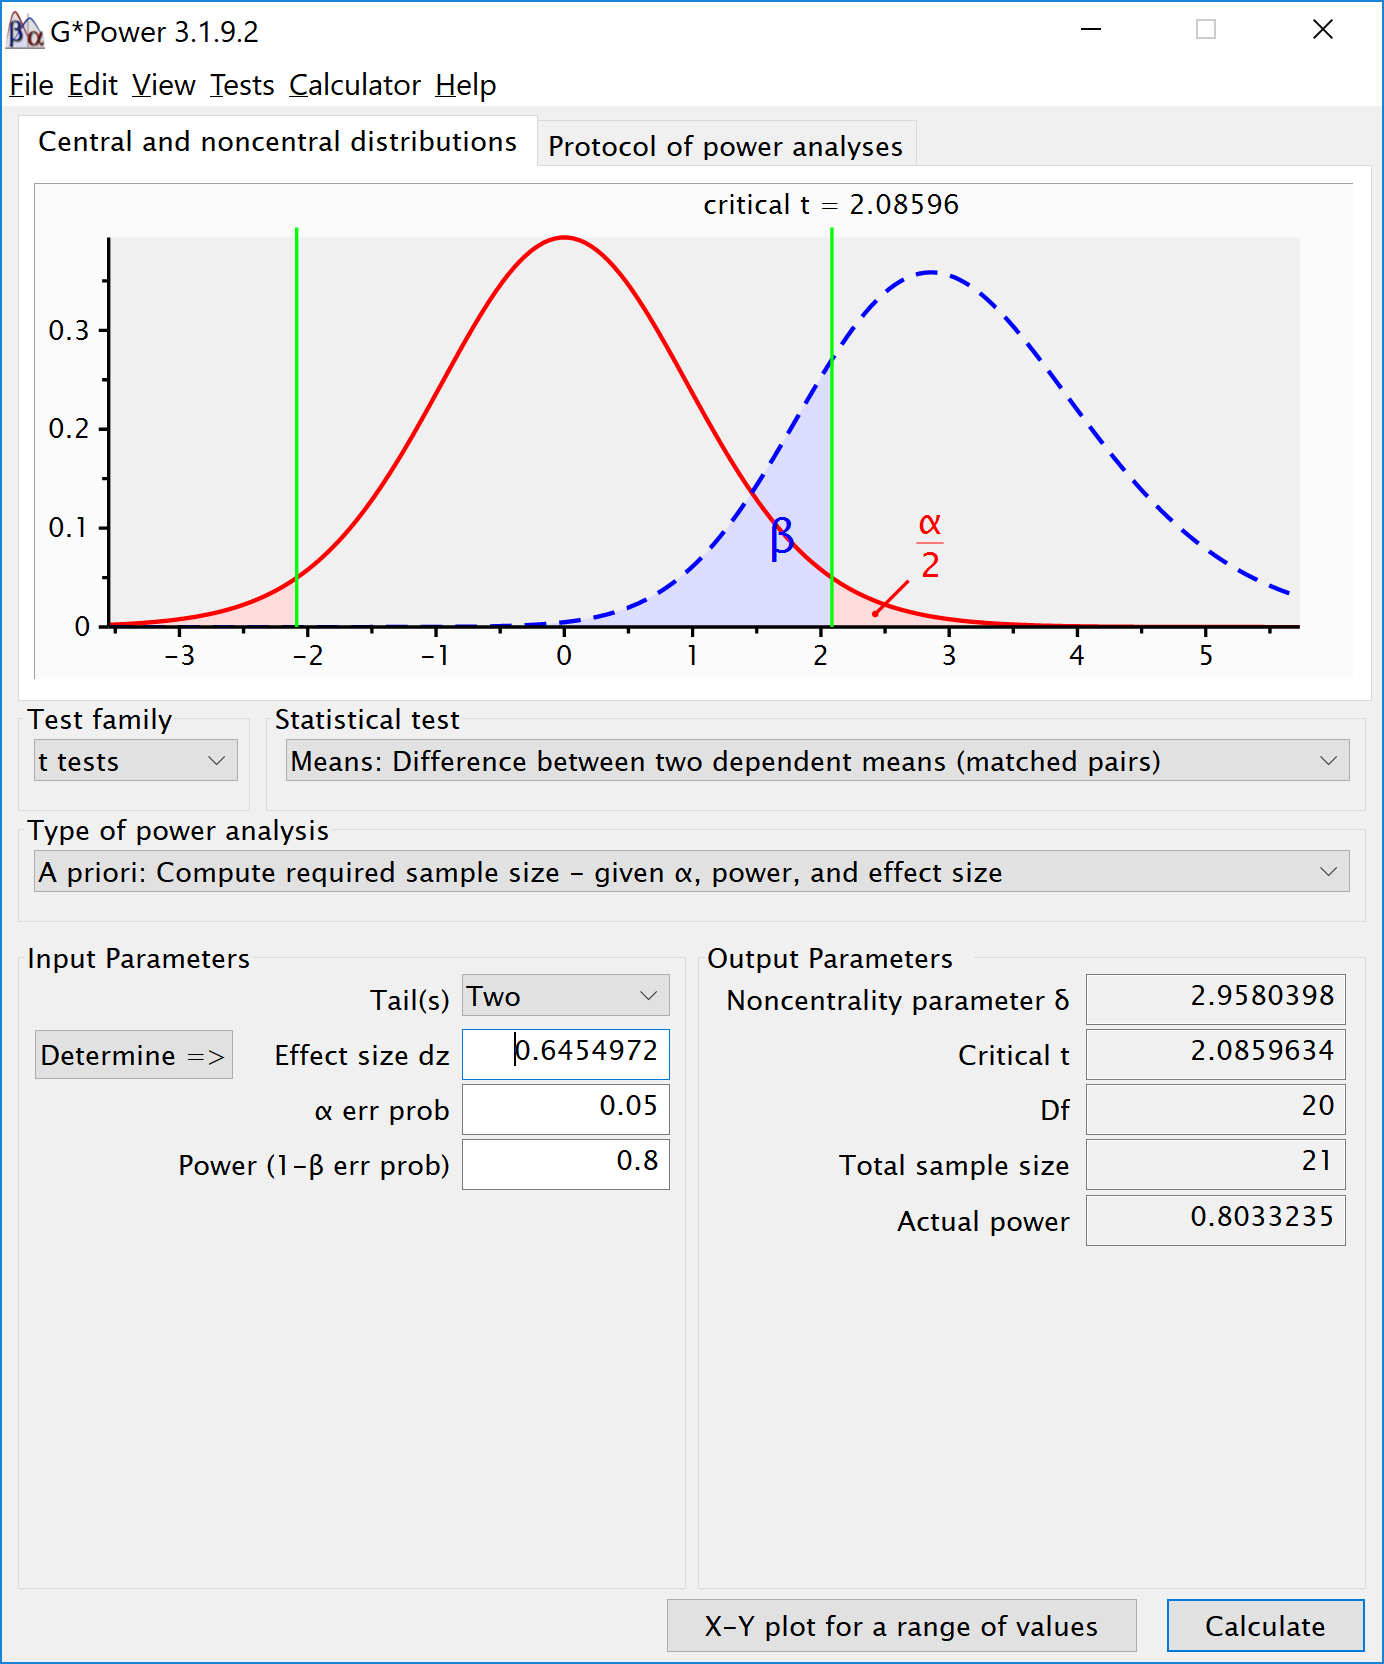
\includegraphics{screenshots/gpower_10.png}

We can perform both these power analyses using simuations as well. We set groups to 2 for the simulation, n = 34 (which should give 80.777 power, according to the g*power program), a correlation among repeated measures of 0.5, and an alpha of 0.05. In this case, we simulate data with means -0.25 and 0.25, and set the sd to 1. This means we have a mean difference of 0.5, and a Cohen's d of 0.5/1 = 0.5. In the first example, we set the correlation to 0.5, and the result should be 80.77\% power, and an effect size estimate of 0.5 for the simple effect. We also calculate partial eta-squared for the ANOVA, which equals \(\frac{f^2}{f^2+1}\), or 0.05882353.

\begin{Shaded}
\begin{Highlighting}[]
\NormalTok{K <-}\StringTok{ }\DecValTok{2}
\NormalTok{n <-}\StringTok{ }\DecValTok{34}
\NormalTok{sd <-}\StringTok{ }\DecValTok{1}
\NormalTok{r <-}\StringTok{ }\FloatTok{0.5}
\NormalTok{alpha =}\StringTok{ }\FloatTok{0.05}
\NormalTok{f <-}\StringTok{ }\FloatTok{0.25}
\NormalTok{f2 <-}\StringTok{ }\NormalTok{f}\OperatorTok{^}\DecValTok{2}
\NormalTok{ES <-}\StringTok{ }\NormalTok{f2}\OperatorTok{/}\NormalTok{(f2}\OperatorTok{+}\DecValTok{1}\NormalTok{)}
\NormalTok{ES}
\end{Highlighting}
\end{Shaded}

\begin{verbatim}
## [1] 0.05882353
\end{verbatim}

\begin{Shaded}
\begin{Highlighting}[]
\NormalTok{mu <-}\StringTok{ }\KeywordTok{mu_from_ES}\NormalTok{(}\DataTypeTok{K =}\NormalTok{ K, }\DataTypeTok{ES =}\NormalTok{ ES)}
\NormalTok{design =}\KeywordTok{paste}\NormalTok{(K,}\StringTok{"w"}\NormalTok{,}\DataTypeTok{sep=}\StringTok{""}\NormalTok{)}
\NormalTok{labelnames <-}\StringTok{ }\KeywordTok{c}\NormalTok{(}\StringTok{"speed"}\NormalTok{, }\StringTok{"fast"}\NormalTok{, }\StringTok{"slow"}\NormalTok{)}
\NormalTok{design_result <-}\StringTok{ }\KeywordTok{ANOVA_design}\NormalTok{(}\DataTypeTok{design =}\NormalTok{ design,}
                   \DataTypeTok{n =}\NormalTok{ n, }
                   \DataTypeTok{mu =}\NormalTok{ mu, }
                   \DataTypeTok{sd =}\NormalTok{ sd, }
                   \DataTypeTok{r =}\NormalTok{ r, }
                   \DataTypeTok{labelnames =}\NormalTok{ labelnames)}
\end{Highlighting}
\end{Shaded}

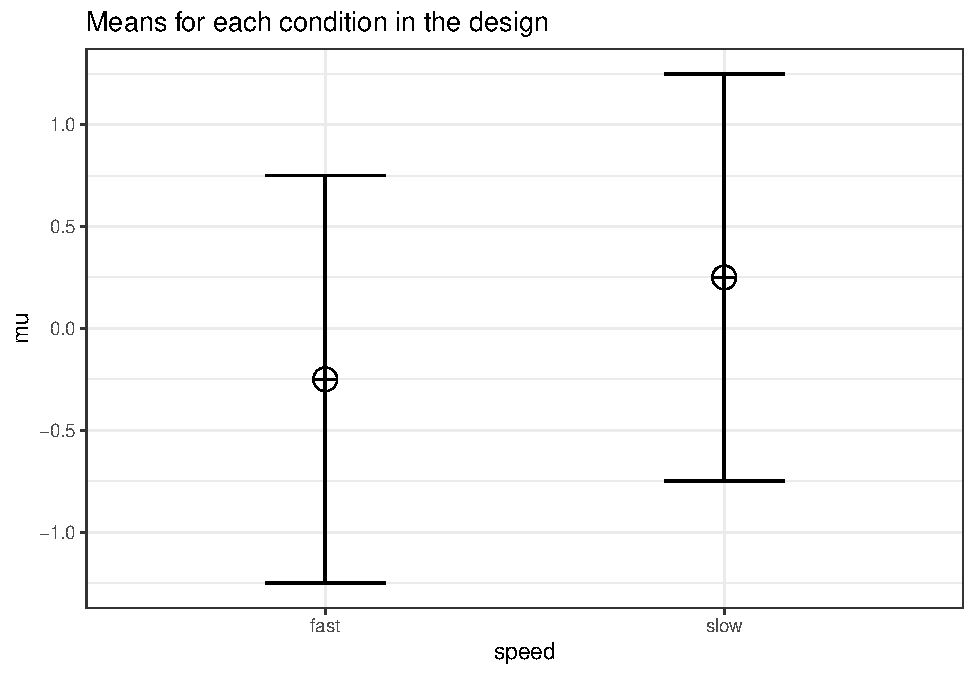
\includegraphics{SuperpowerValidation_files/figure-latex/unnamed-chunk-33-1.pdf}

\begin{Shaded}
\begin{Highlighting}[]
\NormalTok{alpha_level <-}\StringTok{ }\FloatTok{0.05}
\KeywordTok{ANOVA_power}\NormalTok{(design_result, }\DataTypeTok{nsims =}\NormalTok{ nsims)}
\end{Highlighting}
\end{Shaded}

\begin{verbatim}
## Power and Effect sizes for ANOVA tests
##             power effect_size
## anova_speed    80      0.2138
## 
## Power and Effect sizes for contrasts
##                         power effect_size
## p_speed_fast_speed_slow    80      0.5077
## 
## Within-Subject Factors Included: Check MANOVA Results
\end{verbatim}

The results of the simulation are indeed very close to 80.777\%. Note that the simulation calculates Cohen's dz effect sizes for paired comparisons - which here given the correlation of 0.5 is also 0.5 for a medium effect size.

We should see a larger dz if we increase the correlation, keeping the sample size the same, following the example in Gpower above. We repeat the simulation, and the only difference is a correlation between dependent variables of 0.7. This should yield an effect size dz = 0.6454972.

\begin{Shaded}
\begin{Highlighting}[]
\NormalTok{K <-}\StringTok{ }\DecValTok{2}
\NormalTok{n <-}\StringTok{ }\DecValTok{21}
\NormalTok{sd <-}\StringTok{ }\DecValTok{1}
\NormalTok{r <-}\StringTok{ }\FloatTok{0.7}
\NormalTok{alpha =}\StringTok{ }\FloatTok{0.05}
\NormalTok{f <-}\StringTok{ }\FloatTok{0.25}
\NormalTok{f2 <-}\StringTok{ }\NormalTok{f}\OperatorTok{^}\DecValTok{2}
\NormalTok{ES <-}\StringTok{ }\NormalTok{f2}\OperatorTok{/}\NormalTok{(f2}\OperatorTok{+}\DecValTok{1}\NormalTok{)}
\NormalTok{ES}
\end{Highlighting}
\end{Shaded}

\begin{verbatim}
## [1] 0.05882353
\end{verbatim}

\begin{Shaded}
\begin{Highlighting}[]
\NormalTok{mu <-}\StringTok{ }\KeywordTok{mu_from_ES}\NormalTok{(}\DataTypeTok{K =}\NormalTok{ K, }\DataTypeTok{ES =}\NormalTok{ ES)}
\NormalTok{design =}\StringTok{ }\KeywordTok{paste}\NormalTok{(K,}\StringTok{"w"}\NormalTok{,}\DataTypeTok{sep=}\StringTok{""}\NormalTok{)}
\NormalTok{labelnames <-}\StringTok{ }\KeywordTok{c}\NormalTok{(}\StringTok{"speed"}\NormalTok{, }\StringTok{"fast"}\NormalTok{, }\StringTok{"slow"}\NormalTok{)}
\NormalTok{design_result <-}\StringTok{ }\KeywordTok{ANOVA_design}\NormalTok{(}\DataTypeTok{design =}\NormalTok{ design,}
                   \DataTypeTok{n =}\NormalTok{ n, }
                   \DataTypeTok{mu =}\NormalTok{ mu, }
                   \DataTypeTok{sd =}\NormalTok{ sd, }
                   \DataTypeTok{r =}\NormalTok{ r, }
                   \DataTypeTok{labelnames =}\NormalTok{ labelnames)}
\end{Highlighting}
\end{Shaded}

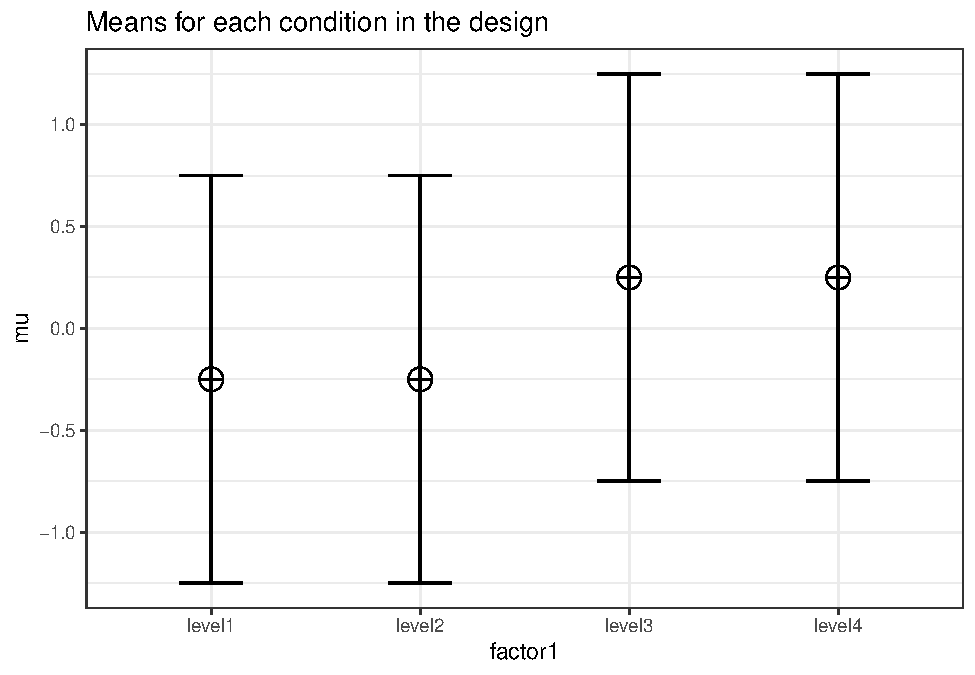
\includegraphics{SuperpowerValidation_files/figure-latex/unnamed-chunk-34-1.pdf}

\begin{Shaded}
\begin{Highlighting}[]
\NormalTok{alpha_level <-}\StringTok{ }\FloatTok{0.05}
\NormalTok{design_result}\OperatorTok{$}\NormalTok{sigmatrix}
\end{Highlighting}
\end{Shaded}

\begin{verbatim}
##      fast slow
## fast  1.0  0.7
## slow  0.7  1.0
\end{verbatim}

\begin{Shaded}
\begin{Highlighting}[]
\KeywordTok{ANOVA_power}\NormalTok{(design_result, }\DataTypeTok{nsims =}\NormalTok{ nsims)}
\end{Highlighting}
\end{Shaded}

\begin{verbatim}
## Power and Effect sizes for ANOVA tests
##             power effect_size
## anova_speed    75      0.2973
## 
## Power and Effect sizes for contrasts
##                         power effect_size
## p_speed_fast_speed_slow    75      0.6434
## 
## Within-Subject Factors Included: Check MANOVA Results
\end{verbatim}

\begin{Shaded}
\begin{Highlighting}[]
\CommentTok{#relation dz and f for within designs }
\NormalTok{f <-}\StringTok{ }\FloatTok{0.5}\OperatorTok{*}\FloatTok{0.6454972}
\CommentTok{# Entering this f in G*power, with a correlation of 0.5, yields the same as entering f = 0.25 and correlation = 0.7. }
\end{Highlighting}
\end{Shaded}

\hypertarget{repeated-measures-anova-part-2}{%
\chapter{Repeated Measures-ANOVA Part 2}\label{repeated-measures-anova-part-2}}

In a repeated measures design multiple observations are collected from the same participants. Here, we will examine a repeated measures experiment with 3 within-subject conditions, to illustrate how a repeated measures ANOVA extends a dependent \emph{t}-test with 3 groups.

In the example for a two-group within design we provided a specific formula for the sample size benefit for two groups. The sample size needed in within-designs (NW) with more than 2 conditions, relative to the sample needed in between-designs (NB), assuming normal distributions and compound symmetry, and ignoring the difference in degrees of freedom between the two types of tests, is (from Maxwell \& Delaney, 2004, p.~562, formula 47):

\(N_{W}=\frac{N_{B}(1-\rho)}{a}\)

Where a is the number of within-subject levels.

\hypertarget{the-relation-between-cohens-f-and-cohens-d}{%
\section{The relation between Cohen's f and Cohen's d}\label{the-relation-between-cohens-f-and-cohens-d}}

Whereas in the case of a repeated measures ANOVA with 2 groups we could explain the principles of a power analysis by comparing our test against a \emph{t}-test and Cohen's d, this becomes more difficult when we have more than 2 groups. It is more useful to explain how to directly calculate Cohen's f, the effect size used in power analyses for ANOVA. Cohen's f is calculated following Cohen, 1988, formula 8.2.1 and 8.2.2:

\(f = \sqrt{\frac{\frac{\sum(\mu-\overline{\mu})^2)}N}\sigma}\)

Imagine we have a within-subject experiment with 3 conditions. We ask people what they mood is when their alarm clock wakes them up, when they wake up naturally on a week day, and when they wake up naturally on a weekend day. Based on pilot data, we expect the means (on a 7 point validated mood scale) are 3.8, 4.2, and 4.3. The standard deviation is 0.9, and the correlation between the dependent measurements is 0.7. We can calculate Cohen's f for the ANOVA, and Cohen's dz for the contrasts:

\begin{Shaded}
\begin{Highlighting}[]
\NormalTok{mu <-}\StringTok{ }\KeywordTok{c}\NormalTok{(}\FloatTok{3.8}\NormalTok{, }\FloatTok{4.2}\NormalTok{, }\FloatTok{4.3}\NormalTok{)}
\NormalTok{sd <-}\StringTok{ }\FloatTok{0.9}
\NormalTok{f <-}\StringTok{ }\KeywordTok{sqrt}\NormalTok{(}\KeywordTok{sum}\NormalTok{((mu}\OperatorTok{-}\KeywordTok{mean}\NormalTok{(mu))}\OperatorTok{^}\DecValTok{2}\NormalTok{)}\OperatorTok{/}\KeywordTok{length}\NormalTok{(mu))}\OperatorTok{/}\NormalTok{sd }\CommentTok{#Cohen, 1988, formula 8.2.1 and 8.2.2}
\NormalTok{f}
\end{Highlighting}
\end{Shaded}

\begin{verbatim}
## [1] 0.2400274
\end{verbatim}

\begin{Shaded}
\begin{Highlighting}[]
\NormalTok{r <-}\StringTok{ }\FloatTok{0.7}
\NormalTok{(}\FloatTok{4.2-3.8}\NormalTok{)}\OperatorTok{/}\FloatTok{0.9}\OperatorTok{/}\KeywordTok{sqrt}\NormalTok{(}\DecValTok{2}\OperatorTok{*}\NormalTok{(}\DecValTok{1}\OperatorTok{-}\NormalTok{r))}
\end{Highlighting}
\end{Shaded}

\begin{verbatim}
## [1] 0.5737753
\end{verbatim}

\begin{Shaded}
\begin{Highlighting}[]
\NormalTok{(}\FloatTok{4.3-3.8}\NormalTok{)}\OperatorTok{/}\FloatTok{0.9}\OperatorTok{/}\KeywordTok{sqrt}\NormalTok{(}\DecValTok{2}\OperatorTok{*}\NormalTok{(}\DecValTok{1}\OperatorTok{-}\NormalTok{r))}
\end{Highlighting}
\end{Shaded}

\begin{verbatim}
## [1] 0.7172191
\end{verbatim}

\begin{Shaded}
\begin{Highlighting}[]
\NormalTok{(}\FloatTok{4.3-4.2}\NormalTok{)}\OperatorTok{/}\FloatTok{0.9}\OperatorTok{/}\KeywordTok{sqrt}\NormalTok{(}\DecValTok{2}\OperatorTok{*}\NormalTok{(}\DecValTok{1}\OperatorTok{-}\NormalTok{r))}
\end{Highlighting}
\end{Shaded}

\begin{verbatim}
## [1] 0.1434438
\end{verbatim}

The relation between Cohen's d or dz and Cohen's f becomes more difficult when there are multiple groups, because the relationship depends on the pattern of the means. Cohen (1988) presents calculations for three patterns, minimal variability (for example, for 5 means: -0.25, 0, 0, 0, 0.25), medium variability (for example, for 5 means: -0.25, -0.25, 0.25, 0.25, 0.25 or -0.25, -0.25, -0.25, 0.25, 0.25). For these three patterns, formula's are available that compute Cohen's f from Cohen's d, where d is the effect size calculated for the difference between the largest and smallest mean (if the largest mean is 0.25 and the smallest mean is -0.25, 0.25 - -0.25 = 0.5, so d is 0.5 divided by the standard deviation of 0.9). In our example, d would be (4.3-3.8)/0.9 = 0.5555556. If we divide this value by sqrt(2*(1-r)) we have dz = 0.5555556/0.7745967 = 0.7172191.

I have created a custom function that will calculate f from d, based on a specification of one of the three patterns of means. Our pattern is most similar (but not identical) to a maximum variability pattern (two means are high, one is lower). So we could attempt to calculate f from d (0.5555556), by calculating d from the largest and smallest mean:

\begin{Shaded}
\begin{Highlighting}[]
\KeywordTok{source}\NormalTok{(}\StringTok{"https://raw.githubusercontent.com/Lakens/ANOVA_power_simulation/master/calc_f_d_eta.R"}\NormalTok{)}
\NormalTok{res <-}\StringTok{ }\KeywordTok{calc_f_d_eta}\NormalTok{(}\DataTypeTok{mu =}\NormalTok{ mu, }\DataTypeTok{sd =}\NormalTok{ sd, }\DataTypeTok{variability =} \StringTok{"maximum"}\NormalTok{)}
\NormalTok{res}\OperatorTok{$}\NormalTok{f}
\end{Highlighting}
\end{Shaded}

\begin{verbatim}
## [1] 0.2618914
\end{verbatim}

\begin{Shaded}
\begin{Highlighting}[]
\NormalTok{res}\OperatorTok{$}\NormalTok{d}
\end{Highlighting}
\end{Shaded}

\begin{verbatim}
## [1] 0.5555556
\end{verbatim}

We see the Cohen's f value is 0.2618914 and d = 0.5555556. The Cohen's f is not perfectly accurate - it is assuming the pattern of means is 3.8, 4.3, 4.3, and not 3.8, 4.2, 4.3. If the means and sd is known, it is best to calculate Cohen's f directly from these values.

\hypertarget{three-within-conditions-medium-effect-size}{%
\section{Three within conditions, medium effect size}\label{three-within-conditions-medium-effect-size}}

We can perform power analyses for within designs using simuations. We set groups to 3 for the simulation, n = 20, and the correlation between dependent variables to 0.8. If the true effect size is f = 0.25, and the alpha level is 0.05, the power is 96.6\%.

In this case, we simulate data with means -0.3061862, 0.0000000, and 0.3061862, and set the sd to 1.

\begin{Shaded}
\begin{Highlighting}[]
\NormalTok{K <-}\StringTok{ }\DecValTok{3}
\NormalTok{n <-}\StringTok{ }\DecValTok{20}
\NormalTok{sd <-}\StringTok{ }\DecValTok{1}
\NormalTok{r <-}\StringTok{ }\FloatTok{0.8}
\NormalTok{alpha =}\StringTok{ }\FloatTok{0.05}
\NormalTok{f <-}\StringTok{ }\FloatTok{0.25}
\NormalTok{f2 <-}\StringTok{ }\NormalTok{f}\OperatorTok{^}\DecValTok{2}
\NormalTok{ES <-}\StringTok{ }\NormalTok{f2}\OperatorTok{/}\NormalTok{(f2}\OperatorTok{+}\DecValTok{1}\NormalTok{)}
\NormalTok{ES}
\end{Highlighting}
\end{Shaded}

\begin{verbatim}
## [1] 0.05882353
\end{verbatim}

\begin{Shaded}
\begin{Highlighting}[]
\NormalTok{mu <-}\StringTok{ }\KeywordTok{mu_from_ES}\NormalTok{(}\DataTypeTok{K =}\NormalTok{ K, }\DataTypeTok{ES =}\NormalTok{ ES)}
\KeywordTok{sqrt}\NormalTok{(}\KeywordTok{sum}\NormalTok{((mu}\OperatorTok{-}\KeywordTok{mean}\NormalTok{(mu))}\OperatorTok{^}\DecValTok{2}\NormalTok{)}\OperatorTok{/}\KeywordTok{length}\NormalTok{(mu))}\OperatorTok{/}\NormalTok{sd }\CommentTok{#Cohen, 1988, formula 8.2.1 and 8.2.2}
\end{Highlighting}
\end{Shaded}

\begin{verbatim}
## [1] 0.25
\end{verbatim}

\begin{Shaded}
\begin{Highlighting}[]
\NormalTok{design =}\KeywordTok{paste}\NormalTok{(K,}\StringTok{"w"}\NormalTok{,}\DataTypeTok{sep=}\StringTok{""}\NormalTok{)}
\NormalTok{labelnames <-}\StringTok{ }\KeywordTok{c}\NormalTok{(}\StringTok{"speed"}\NormalTok{, }\StringTok{"fast"}\NormalTok{, }\StringTok{"medium"}\NormalTok{, }\StringTok{"slow"}\NormalTok{)}
\NormalTok{design_result <-}\StringTok{ }\KeywordTok{ANOVA_design}\NormalTok{(}\DataTypeTok{design =}\NormalTok{ design,}
                   \DataTypeTok{n =}\NormalTok{ n, }
                   \DataTypeTok{mu =}\NormalTok{ mu, }
                   \DataTypeTok{sd =}\NormalTok{ sd, }
                   \DataTypeTok{r =}\NormalTok{ r, }
                   \DataTypeTok{labelnames =}\NormalTok{ labelnames)}
\end{Highlighting}
\end{Shaded}

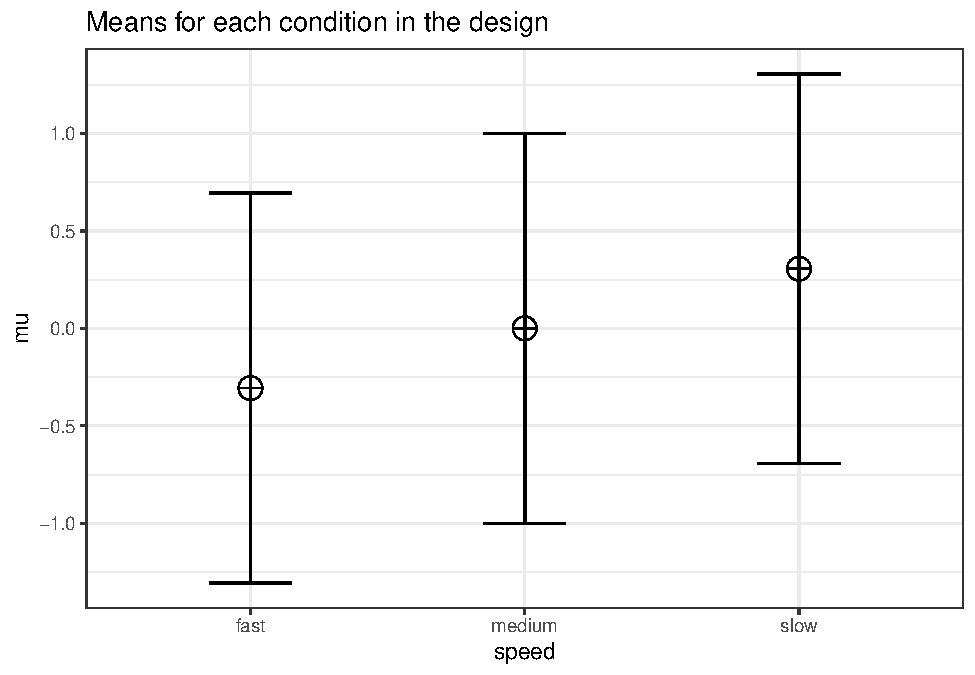
\includegraphics{SuperpowerValidation_files/figure-latex/unnamed-chunk-38-1.pdf}

\begin{Shaded}
\begin{Highlighting}[]
\NormalTok{alpha_level <-}\StringTok{ }\FloatTok{0.05}
\KeywordTok{ANOVA_power}\NormalTok{(design_result, }\DataTypeTok{nsims =}\NormalTok{ nsims)}
\end{Highlighting}
\end{Shaded}

\begin{verbatim}
## Power and Effect sizes for ANOVA tests
##             power effect_size
## anova_speed    95      0.3583
## 
## Power and Effect sizes for contrasts
##                           power effect_size
## p_speed_fast_speed_medium    60      0.5350
## p_speed_fast_speed_slow      97      1.0342
## p_speed_medium_speed_slow    53      0.5059
## 
## Within-Subject Factors Included: Check MANOVA Results
\end{verbatim}

The results of the simulation are indeed very close to 96.9\%. We can see this is in line with the power estimate from Gpower:

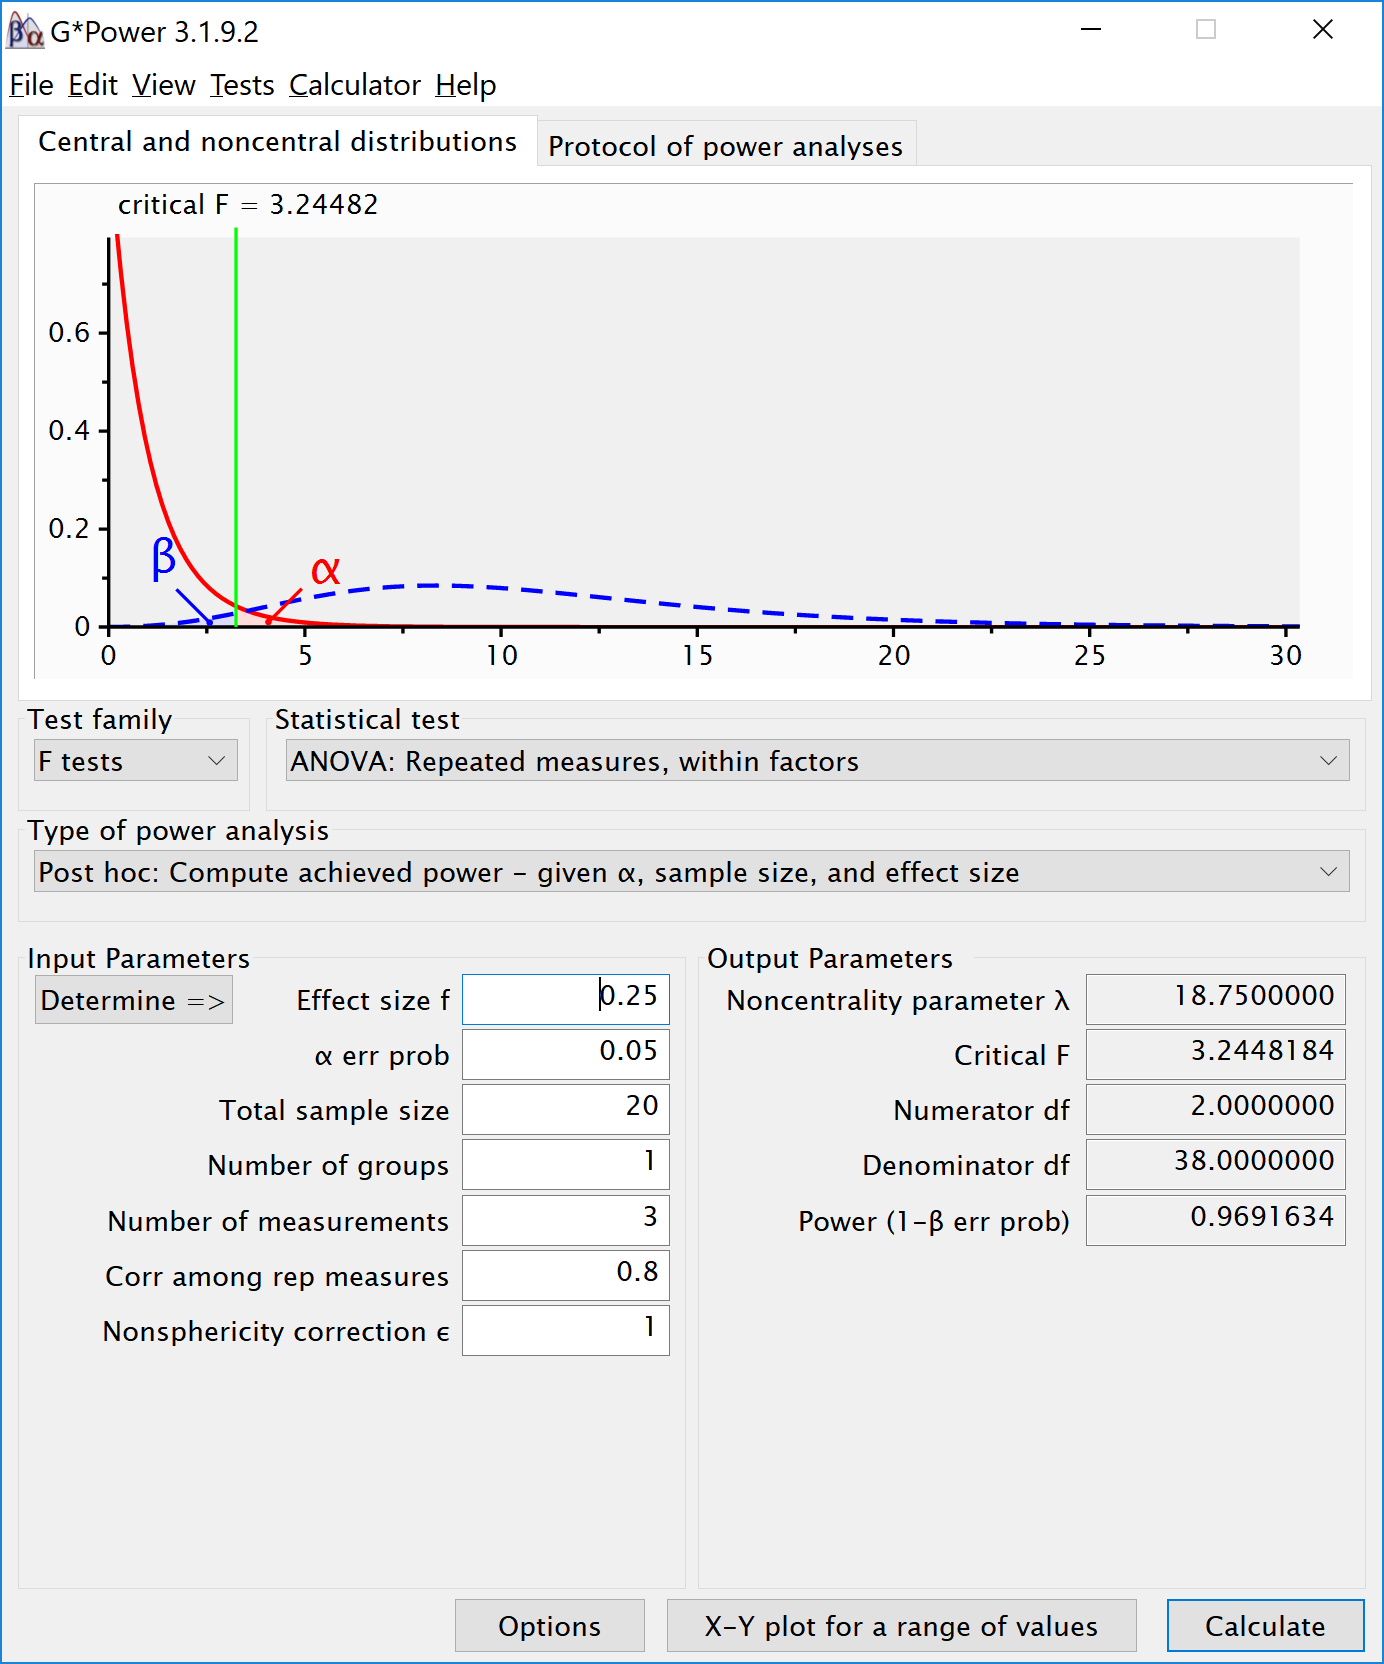
\includegraphics{screenshots/gpower_12.png}

We can also validate this by creating the code to do a power analysis in R from scratch:

\begin{Shaded}
\begin{Highlighting}[]
\NormalTok{K <-}\StringTok{ }\DecValTok{3} \CommentTok{#three groups}
\NormalTok{n <-}\StringTok{ }\DecValTok{20}
\NormalTok{sd <-}\StringTok{ }\DecValTok{1}
\NormalTok{r <-}\StringTok{ }\FloatTok{0.8}
\NormalTok{alpha =}\StringTok{ }\FloatTok{0.05}
\NormalTok{f <-}\StringTok{ }\FloatTok{0.25}
\NormalTok{f2 <-}\StringTok{ }\NormalTok{f}\OperatorTok{^}\DecValTok{2}
\NormalTok{ES <-}\StringTok{ }\NormalTok{f2}\OperatorTok{/}\NormalTok{(f2}\OperatorTok{+}\DecValTok{1}\NormalTok{)}
\NormalTok{ES}
\end{Highlighting}
\end{Shaded}

\begin{verbatim}
## [1] 0.05882353
\end{verbatim}

\begin{Shaded}
\begin{Highlighting}[]
\NormalTok{mu <-}\StringTok{ }\KeywordTok{mu_from_ES}\NormalTok{(}\DataTypeTok{K =}\NormalTok{ K, }\DataTypeTok{ES =}\NormalTok{ ES)}
\NormalTok{design =}\KeywordTok{paste}\NormalTok{(K,}\StringTok{"w"}\NormalTok{,}\DataTypeTok{sep=}\StringTok{""}\NormalTok{)}
\NormalTok{labelnames <-}\StringTok{ }\KeywordTok{c}\NormalTok{(}\StringTok{"speed"}\NormalTok{, }\StringTok{"fast"}\NormalTok{, }\StringTok{"medium"}\NormalTok{, }\StringTok{"slow"}\NormalTok{)}
\NormalTok{design_result <-}\StringTok{ }\KeywordTok{ANOVA_design}\NormalTok{(}\DataTypeTok{design =}\NormalTok{ design,}
                   \DataTypeTok{n =}\NormalTok{ n, }
                   \DataTypeTok{mu =}\NormalTok{ mu, }
                   \DataTypeTok{sd =}\NormalTok{ sd, }
                   \DataTypeTok{r =}\NormalTok{ r, }
                   \DataTypeTok{labelnames =}\NormalTok{ labelnames)}
\end{Highlighting}
\end{Shaded}

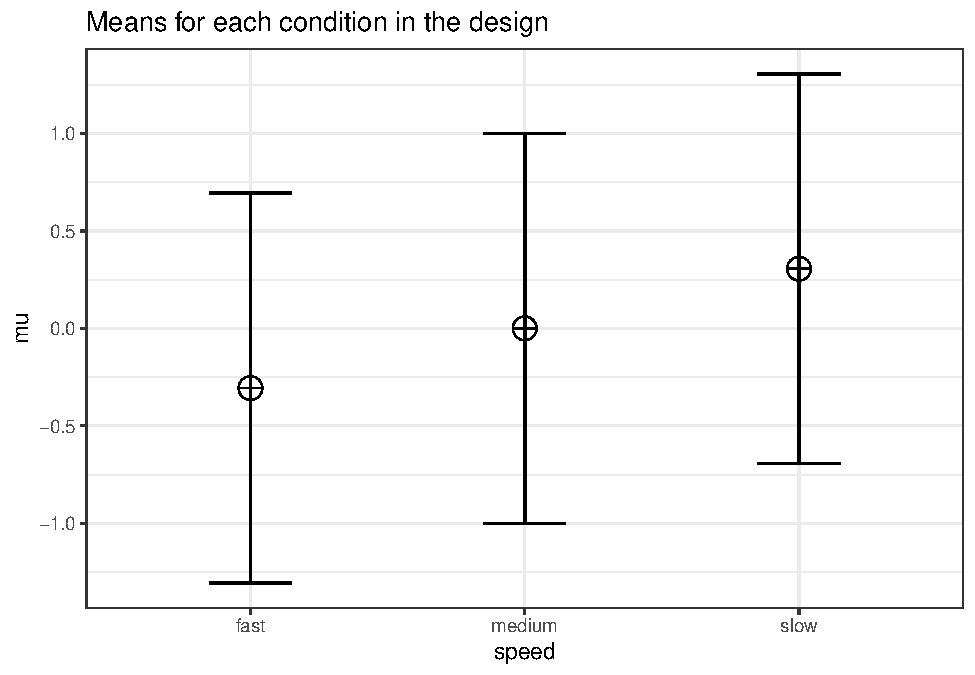
\includegraphics{SuperpowerValidation_files/figure-latex/unnamed-chunk-39-1.pdf}

\begin{Shaded}
\begin{Highlighting}[]
\KeywordTok{power_oneway_within}\NormalTok{(design_result)}\OperatorTok{$}\NormalTok{power}
\end{Highlighting}
\end{Shaded}

\begin{verbatim}
## [1] 0.9691634
\end{verbatim}

\begin{Shaded}
\begin{Highlighting}[]
\KeywordTok{power_oneway_within}\NormalTok{(design_result)}\OperatorTok{$}\NormalTok{eta_p_}\DecValTok{2}
\end{Highlighting}
\end{Shaded}

\begin{verbatim}
## [1] 0.05882353
\end{verbatim}

\begin{Shaded}
\begin{Highlighting}[]
\KeywordTok{power_oneway_within}\NormalTok{(design_result)}\OperatorTok{$}\NormalTok{eta_p_}\DecValTok{2}\NormalTok{_SPSS}
\end{Highlighting}
\end{Shaded}

\begin{verbatim}
## [1] 0.3303965
\end{verbatim}

\begin{Shaded}
\begin{Highlighting}[]
\KeywordTok{power_oneway_within}\NormalTok{(design_result)}\OperatorTok{$}\NormalTok{Cohen_f}
\end{Highlighting}
\end{Shaded}

\begin{verbatim}
## [1] 0.25
\end{verbatim}

\begin{Shaded}
\begin{Highlighting}[]
\KeywordTok{power_oneway_within}\NormalTok{(design_result)}\OperatorTok{$}\NormalTok{Cohen_f_SPSS}
\end{Highlighting}
\end{Shaded}

\begin{verbatim}
## [1] 0.7024394
\end{verbatim}

We can even check the calculation of Cohen's f SPSS style in GPower. We take the GPower settings as illustrated above. We click the `Options' button, and check the radiobutton next to `As in SPSS'. Click ok, and you will notice that the `Corr among rep measures' field has disappeared. The correlation does not need to be entered seperately, but is incorporated in Cohen's f.~The value of Cohen's f, which was 0.25, has changed into 0.7024394. This is the SPSS equivalent. The value is much larger. This value, and it's corresponding partial eta-squared, incorporate the correlation between observations.

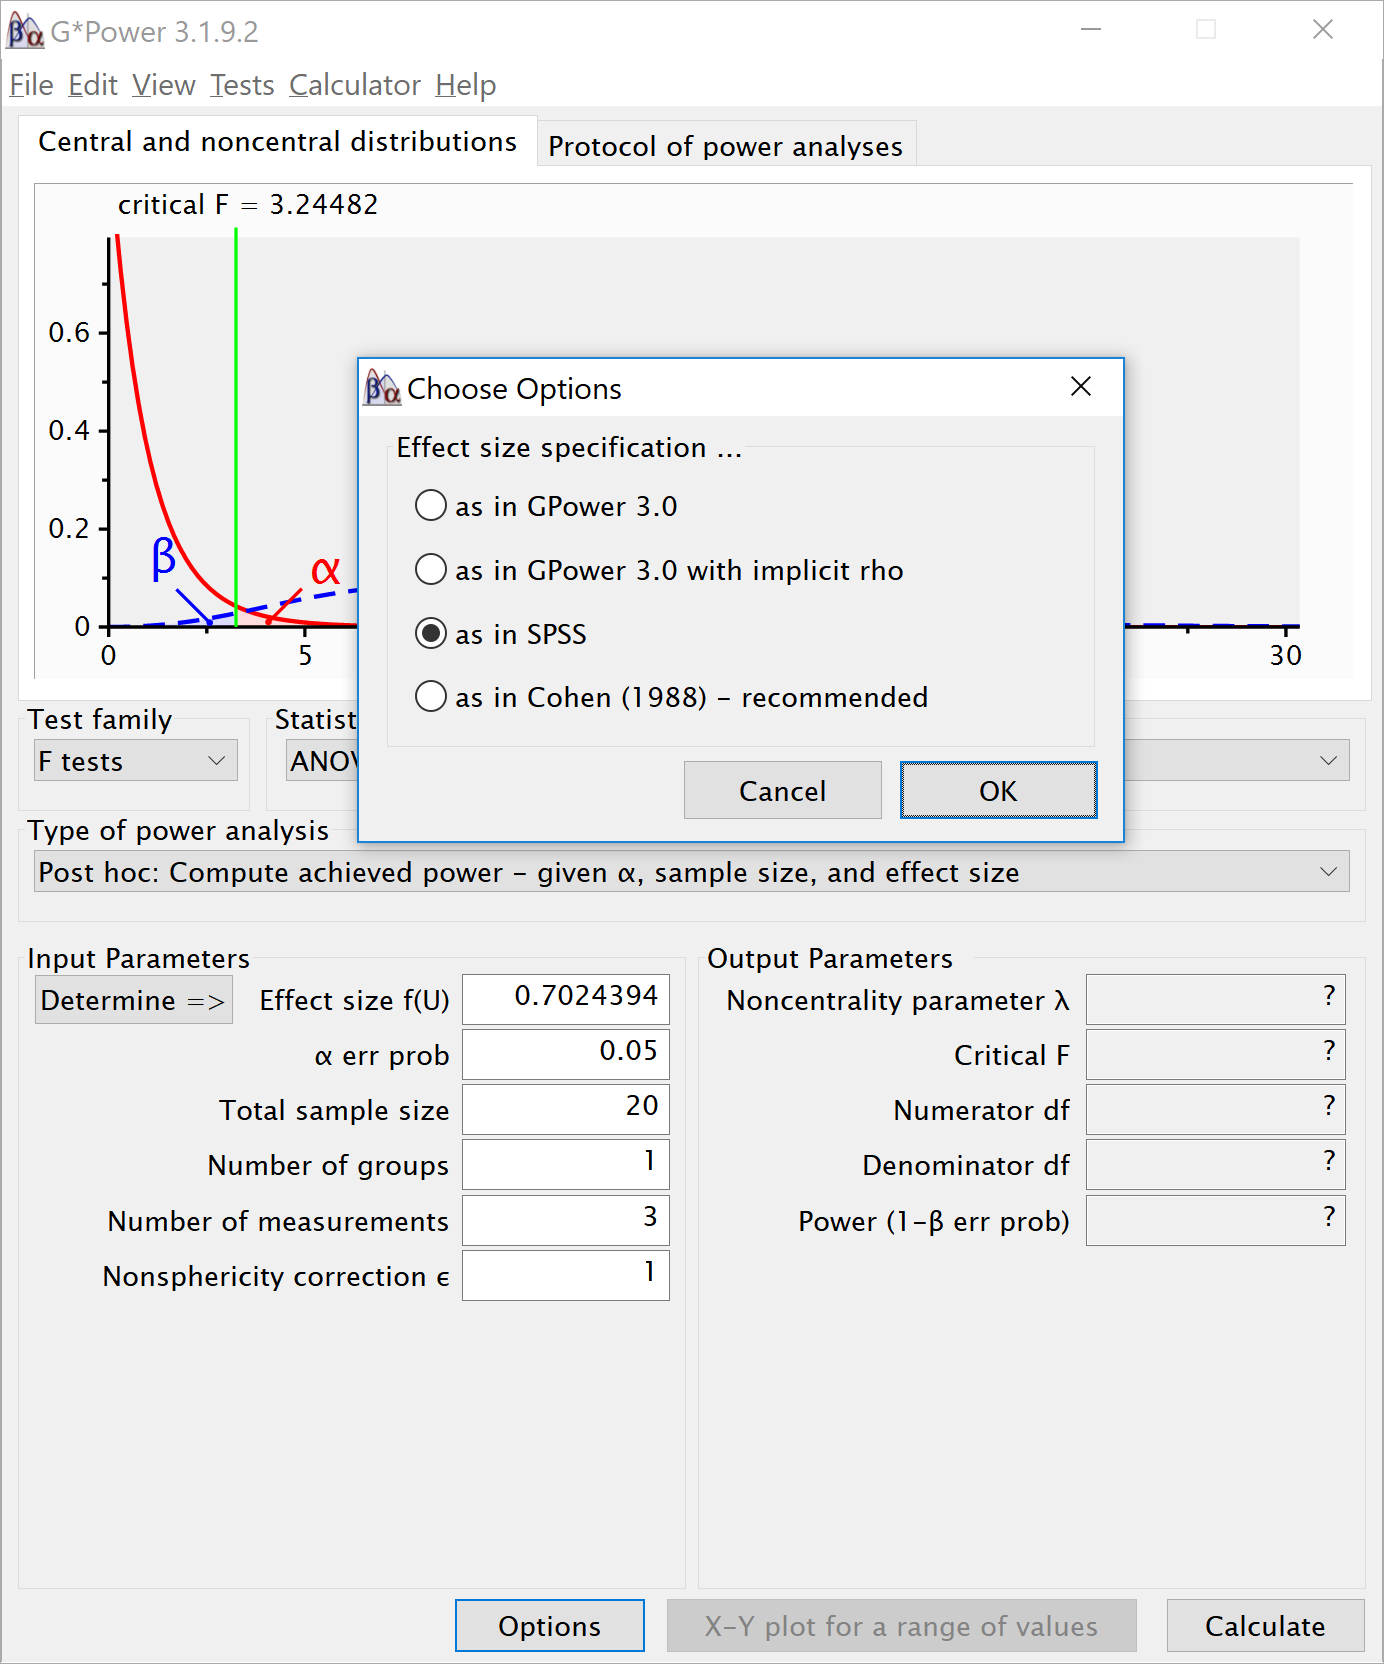
\includegraphics{screenshots/gpower_14.png}

\hypertarget{repeated-measures-anova-part-3}{%
\chapter{Repeated Measures-ANOVA Part 3}\label{repeated-measures-anova-part-3}}

We first repeat the simulation by Brysbaert:

\begin{Shaded}
\begin{Highlighting}[]
\CommentTok{# give sample size}
\NormalTok{N =}\StringTok{ }\DecValTok{75}
\CommentTok{# give effect size d}
\NormalTok{d1 =}\StringTok{ }\FloatTok{.4} \CommentTok{#difference between the extremes}
\NormalTok{d2 =}\StringTok{ }\FloatTok{.4} \CommentTok{#third condition goes with the highest extreme}
\CommentTok{# give the correlation between the conditions}
\NormalTok{r =}\StringTok{ }\FloatTok{.5}
\CommentTok{# give number of simulations}
\NormalTok{nSim =}\StringTok{ }\NormalTok{nsims}
\CommentTok{# give alpha levels}
\NormalTok{alpha1 =}\StringTok{ }\FloatTok{.05} \CommentTok{#alpha level for the omnibus ANOVA}
\NormalTok{alpha2 =}\StringTok{ }\FloatTok{.05} \CommentTok{#also adjusted from original by DL}
\CommentTok{# create progress bar in case it takes a while}
\CommentTok{#pb <- winProgressBar(title = "progress bar", min = 0, max = nSim, width = 300)}
\CommentTok{# create vectors to store p-values}
\NormalTok{p1 <-}\KeywordTok{numeric}\NormalTok{(nSim) }\CommentTok{#p-value omnibus ANOVA}
\NormalTok{p2 <-}\KeywordTok{numeric}\NormalTok{(nSim) }\CommentTok{#p-value first post hoc test}
\NormalTok{p3 <-}\KeywordTok{numeric}\NormalTok{(nSim) }\CommentTok{#p-value second post hoc test}
\NormalTok{p4 <-}\KeywordTok{numeric}\NormalTok{(nSim) }\CommentTok{#p-value third post hoc test}
\CommentTok{# open library MASS}
\KeywordTok{library}\NormalTok{(}\StringTok{'MASS'}\NormalTok{)}
\CommentTok{# define correlation matrix}
\NormalTok{rho <-}\StringTok{ }\KeywordTok{cbind}\NormalTok{(}\KeywordTok{c}\NormalTok{(}\DecValTok{1}\NormalTok{, r, r), }\KeywordTok{c}\NormalTok{(r, }\DecValTok{1}\NormalTok{, r), }\KeywordTok{c}\NormalTok{(r, r, }\DecValTok{1}\NormalTok{))}
\CommentTok{# define participant codes}
\NormalTok{part <-}\StringTok{ }\KeywordTok{paste}\NormalTok{(}\StringTok{"part"}\NormalTok{,}\KeywordTok{seq}\NormalTok{(}\DecValTok{1}\OperatorTok{:}\NormalTok{N))}
\ControlFlowTok{for}\NormalTok{(i }\ControlFlowTok{in} \DecValTok{1}\OperatorTok{:}\NormalTok{nSim)\{ }\CommentTok{#for each simulated experiment}
 \CommentTok{# setWinProgressBar(pb, i, title=paste(round(i/nSim*100, 1), "% done"))}
\NormalTok{  data =}\StringTok{ }\KeywordTok{mvrnorm}\NormalTok{(}\DataTypeTok{n=}\NormalTok{N, }\DataTypeTok{mu=}\KeywordTok{c}\NormalTok{(}\DecValTok{0}\NormalTok{, }\DecValTok{0}\NormalTok{, }\DecValTok{0}\NormalTok{), }\DataTypeTok{Sigma=}\NormalTok{rho)}
\NormalTok{  data[,}\DecValTok{2}\NormalTok{] =}\StringTok{ }\NormalTok{data[,}\DecValTok{2}\NormalTok{]}\OperatorTok{+}\NormalTok{d1}
\NormalTok{  data[,}\DecValTok{3}\NormalTok{] =}\StringTok{ }\NormalTok{data[,}\DecValTok{3}\NormalTok{]}\OperatorTok{+}\NormalTok{d2}
\NormalTok{  datalong =}\StringTok{ }\KeywordTok{c}\NormalTok{(data[,}\DecValTok{1}\NormalTok{],data[,}\DecValTok{2}\NormalTok{],data[,}\DecValTok{3}\NormalTok{])}
\NormalTok{  conds=}\StringTok{ }\KeywordTok{factor}\NormalTok{(}\KeywordTok{rep}\NormalTok{(letters[}\DecValTok{24}\OperatorTok{:}\DecValTok{26}\NormalTok{], }\DataTypeTok{each =}\NormalTok{ N))}
\NormalTok{  partID =}\StringTok{ }\KeywordTok{factor}\NormalTok{(}\KeywordTok{rep}\NormalTok{(part, }\DataTypeTok{times =} \DecValTok{3}\NormalTok{))}
\NormalTok{  output <-}\KeywordTok{data.frame}\NormalTok{(partID,conds,datalong)}
\NormalTok{  test <-}\StringTok{ }\KeywordTok{aov}\NormalTok{(datalong}\OperatorTok{~}\NormalTok{conds }\OperatorTok{+}\StringTok{ }\KeywordTok{Error}\NormalTok{(partID}\OperatorTok{/}\NormalTok{conds), }\DataTypeTok{data=}\NormalTok{output)}
\NormalTok{  tests <-}\StringTok{ }\NormalTok{(}\KeywordTok{summary}\NormalTok{(test))}
\NormalTok{  p1[i] <-}\StringTok{ }\NormalTok{tests}\OperatorTok{$}\StringTok{'Error: partID:conds'}\NormalTok{[[}\DecValTok{1}\NormalTok{]]}\OperatorTok{$}\StringTok{'Pr(>F)'}\NormalTok{[[}\DecValTok{1}\NormalTok{]]}
\NormalTok{  p2[i] <-}\StringTok{ }\KeywordTok{t.test}\NormalTok{(data[,}\DecValTok{1}\NormalTok{],data[,}\DecValTok{2}\NormalTok{], }\DataTypeTok{paired=}\OtherTok{TRUE}\NormalTok{)}\OperatorTok{$}\NormalTok{p.value}
\NormalTok{  p3[i] <-}\StringTok{ }\KeywordTok{t.test}\NormalTok{(data[,}\DecValTok{1}\NormalTok{],data[,}\DecValTok{3}\NormalTok{], }\DataTypeTok{paired=}\OtherTok{TRUE}\NormalTok{)}\OperatorTok{$}\NormalTok{p.value}
\NormalTok{  p4[i] <-}\StringTok{ }\KeywordTok{t.test}\NormalTok{(data[,}\DecValTok{2}\NormalTok{],data[,}\DecValTok{3}\NormalTok{], }\DataTypeTok{paired=}\OtherTok{TRUE}\NormalTok{)}\OperatorTok{$}\NormalTok{p.value}
\NormalTok{  \}}
\CommentTok{#close(pb)#close progress bar}
\CommentTok{#printing all unique tests (adjusted code by DL)}
\KeywordTok{sum}\NormalTok{(p1}\OperatorTok{<}\NormalTok{alpha1)}\OperatorTok{/}\NormalTok{nSim}
\end{Highlighting}
\end{Shaded}

\begin{verbatim}
## [1] 0.94
\end{verbatim}

\begin{Shaded}
\begin{Highlighting}[]
\KeywordTok{sum}\NormalTok{(p2}\OperatorTok{<}\NormalTok{alpha2)}\OperatorTok{/}\NormalTok{nSim}
\end{Highlighting}
\end{Shaded}

\begin{verbatim}
## [1] 0.94
\end{verbatim}

\begin{Shaded}
\begin{Highlighting}[]
\KeywordTok{sum}\NormalTok{(p3}\OperatorTok{<}\NormalTok{alpha2)}\OperatorTok{/}\NormalTok{nSim}
\end{Highlighting}
\end{Shaded}

\begin{verbatim}
## [1] 0.93
\end{verbatim}

\begin{Shaded}
\begin{Highlighting}[]
\KeywordTok{sum}\NormalTok{(p4}\OperatorTok{<}\NormalTok{alpha2)}\OperatorTok{/}\NormalTok{nSim}
\end{Highlighting}
\end{Shaded}

\begin{verbatim}
## [1] 0.01
\end{verbatim}

\hypertarget{reproducing-brysbaert}{%
\section{Reproducing Brysbaert}\label{reproducing-brysbaert}}

We can reproduce the same results as Brysbaeert finds with his code:

\begin{Shaded}
\begin{Highlighting}[]
\NormalTok{design <-}\StringTok{ "3w"}
\NormalTok{n <-}\StringTok{ }\DecValTok{75}
\NormalTok{mu <-}\StringTok{ }\KeywordTok{c}\NormalTok{(}\DecValTok{0}\NormalTok{, }\FloatTok{0.4}\NormalTok{, }\FloatTok{0.4}\NormalTok{)}
\NormalTok{sd <-}\StringTok{ }\DecValTok{1}
\NormalTok{r <-}\StringTok{ }\FloatTok{0.5}
\NormalTok{labelnames <-}\StringTok{ }\KeywordTok{c}\NormalTok{(}\StringTok{"speed"}\NormalTok{, }\StringTok{"fast"}\NormalTok{, }\StringTok{"medium"}\NormalTok{, }\StringTok{"slow"}\NormalTok{)}
\end{Highlighting}
\end{Shaded}

We create the within design, and run the simulation

\begin{Shaded}
\begin{Highlighting}[]
\NormalTok{design_result <-}\StringTok{ }\KeywordTok{ANOVA_design}\NormalTok{(}\DataTypeTok{design =}\NormalTok{ design,}
                   \DataTypeTok{n =}\NormalTok{ n, }
                   \DataTypeTok{mu =}\NormalTok{ mu, }
                   \DataTypeTok{sd =}\NormalTok{ sd, }
                   \DataTypeTok{r =}\NormalTok{ r, }
                   \DataTypeTok{labelnames =}\NormalTok{ labelnames)}
\end{Highlighting}
\end{Shaded}

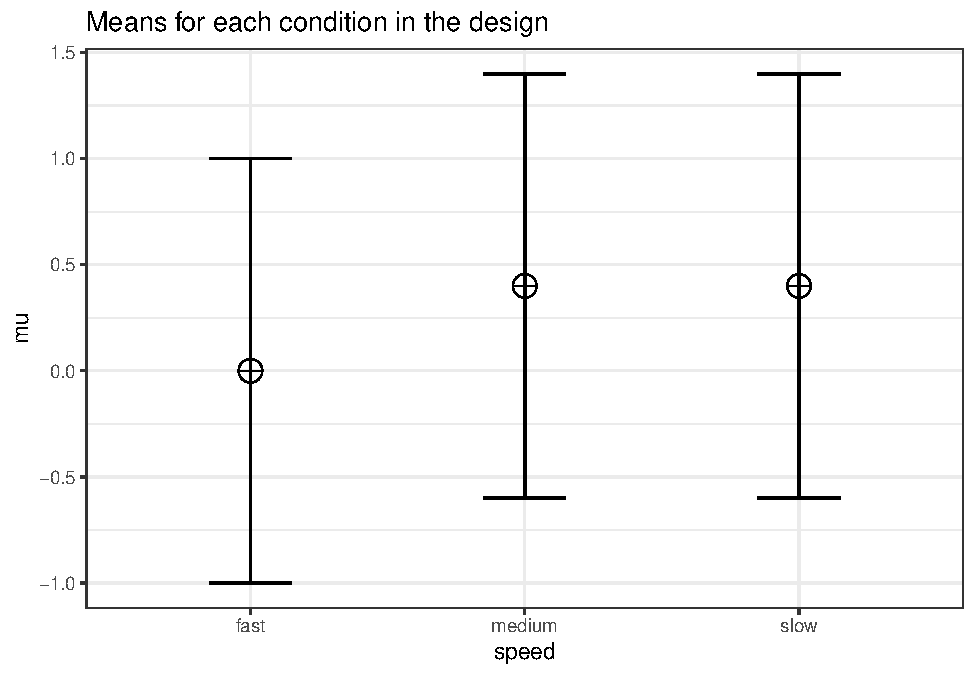
\includegraphics{SuperpowerValidation_files/figure-latex/unnamed-chunk-42-1.pdf}

\begin{Shaded}
\begin{Highlighting}[]
\KeywordTok{ANOVA_power}\NormalTok{(design_result, }\DataTypeTok{nsims =}\NormalTok{ nsims)}
\end{Highlighting}
\end{Shaded}

\begin{verbatim}
## Power and Effect sizes for ANOVA tests
##             power effect_size
## anova_speed    94     0.09853
## 
## Power and Effect sizes for contrasts
##                           power effect_size
## p_speed_fast_speed_medium    91      0.3842
## p_speed_fast_speed_slow      93      0.3887
## p_speed_medium_speed_slow     6      0.0078
## 
## Within-Subject Factors Included: Check MANOVA Results
\end{verbatim}

\#Results

The results of the simulation are very similar. Power for the ANOVA \emph{F}-test is around 95.2\%. For the three paired t-tests, power is around 92.7. This is in line with the a-priori power analysis when using g*power:

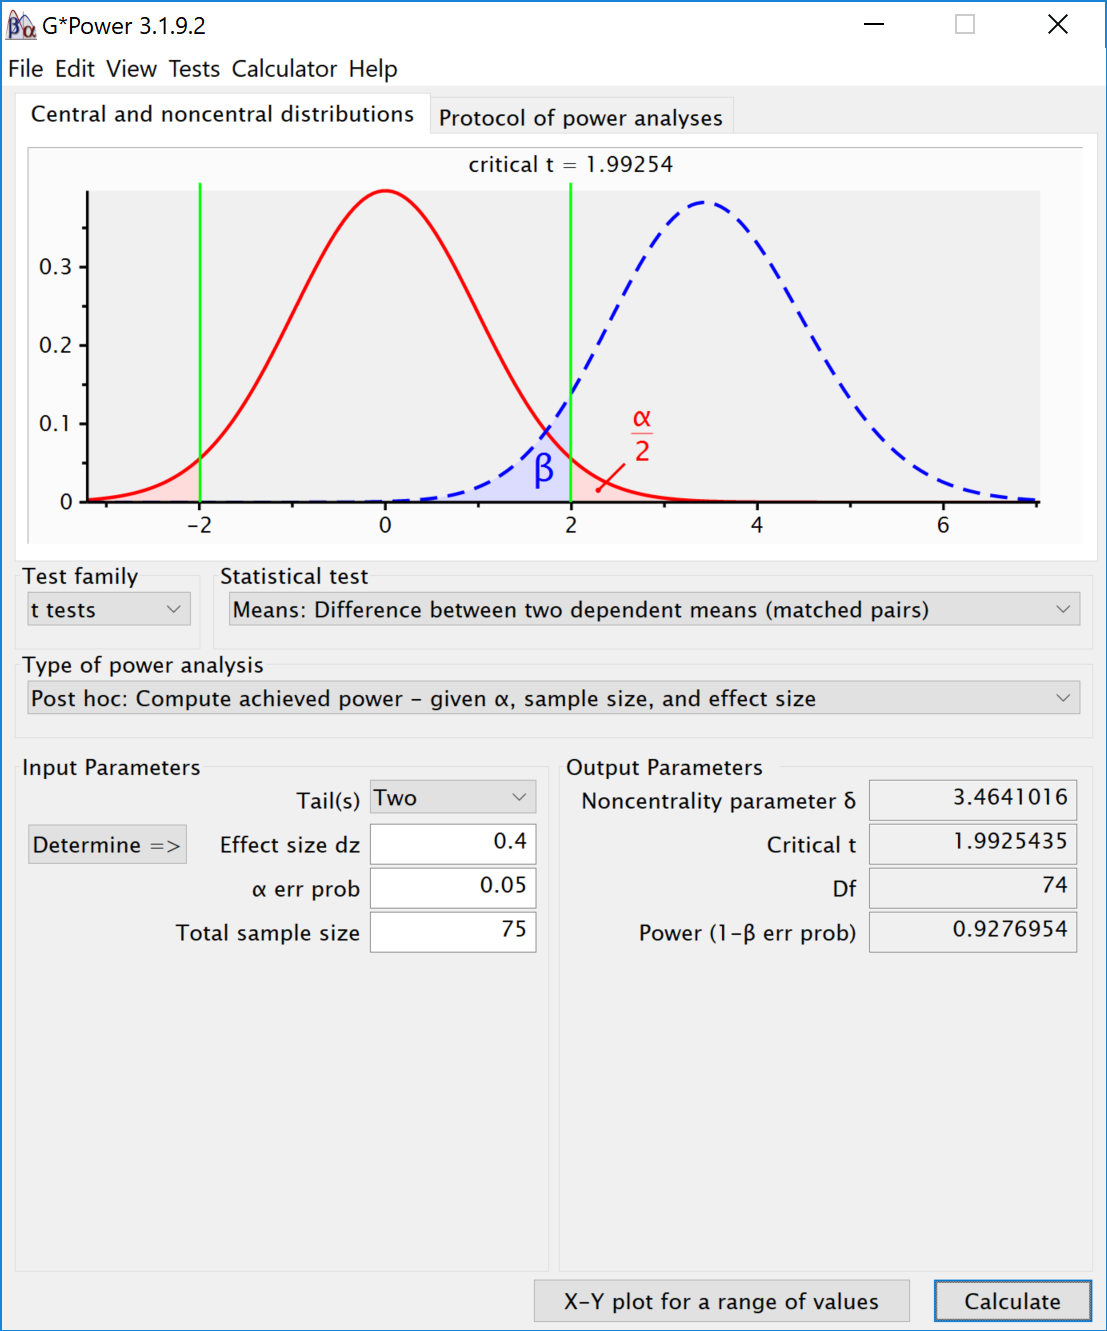
\includegraphics{screenshots/gpower_2.png}

We can perform an post-hoc power analysis in G*power. We can calculate Cohen´s f based on the means and sd, using our own custom formula.

\begin{Shaded}
\begin{Highlighting}[]
\CommentTok{# Our simulation is based onthe following means and sd:}
\CommentTok{# mu <- c(0, 0.4, 0.4)}
\CommentTok{# sd <- 1}
\NormalTok{f <-}\StringTok{ }\KeywordTok{sqrt}\NormalTok{(}\KeywordTok{sum}\NormalTok{((mu}\OperatorTok{-}\KeywordTok{mean}\NormalTok{(mu))}\OperatorTok{^}\DecValTok{2}\NormalTok{)}\OperatorTok{/}\KeywordTok{length}\NormalTok{(mu))}\OperatorTok{/}\NormalTok{sd }\CommentTok{#Cohen, 1988, formula 8.2.1 and 8.2.2}
\CommentTok{# We can see why f = 0.5*d. }
\CommentTok{# Imagine 2 group, mu = 1 and 2}
\CommentTok{# Grand mean is 1.5, we have sqrt(sum(0.5^2 + 0.5^2)/2), or sqrt(0.5/2), = 0.5. }
\CommentTok{# For Cohen's d we use the difference, 2-1 = 1. }
\end{Highlighting}
\end{Shaded}

The Cohen´s f is 0.1885618. We can enter the f (using the default 'as in G*Power 3.0' in the option window) and enter a sample size of 75, number of groups as 1, number of measurements as 3, correlation as 0.5. This yields:

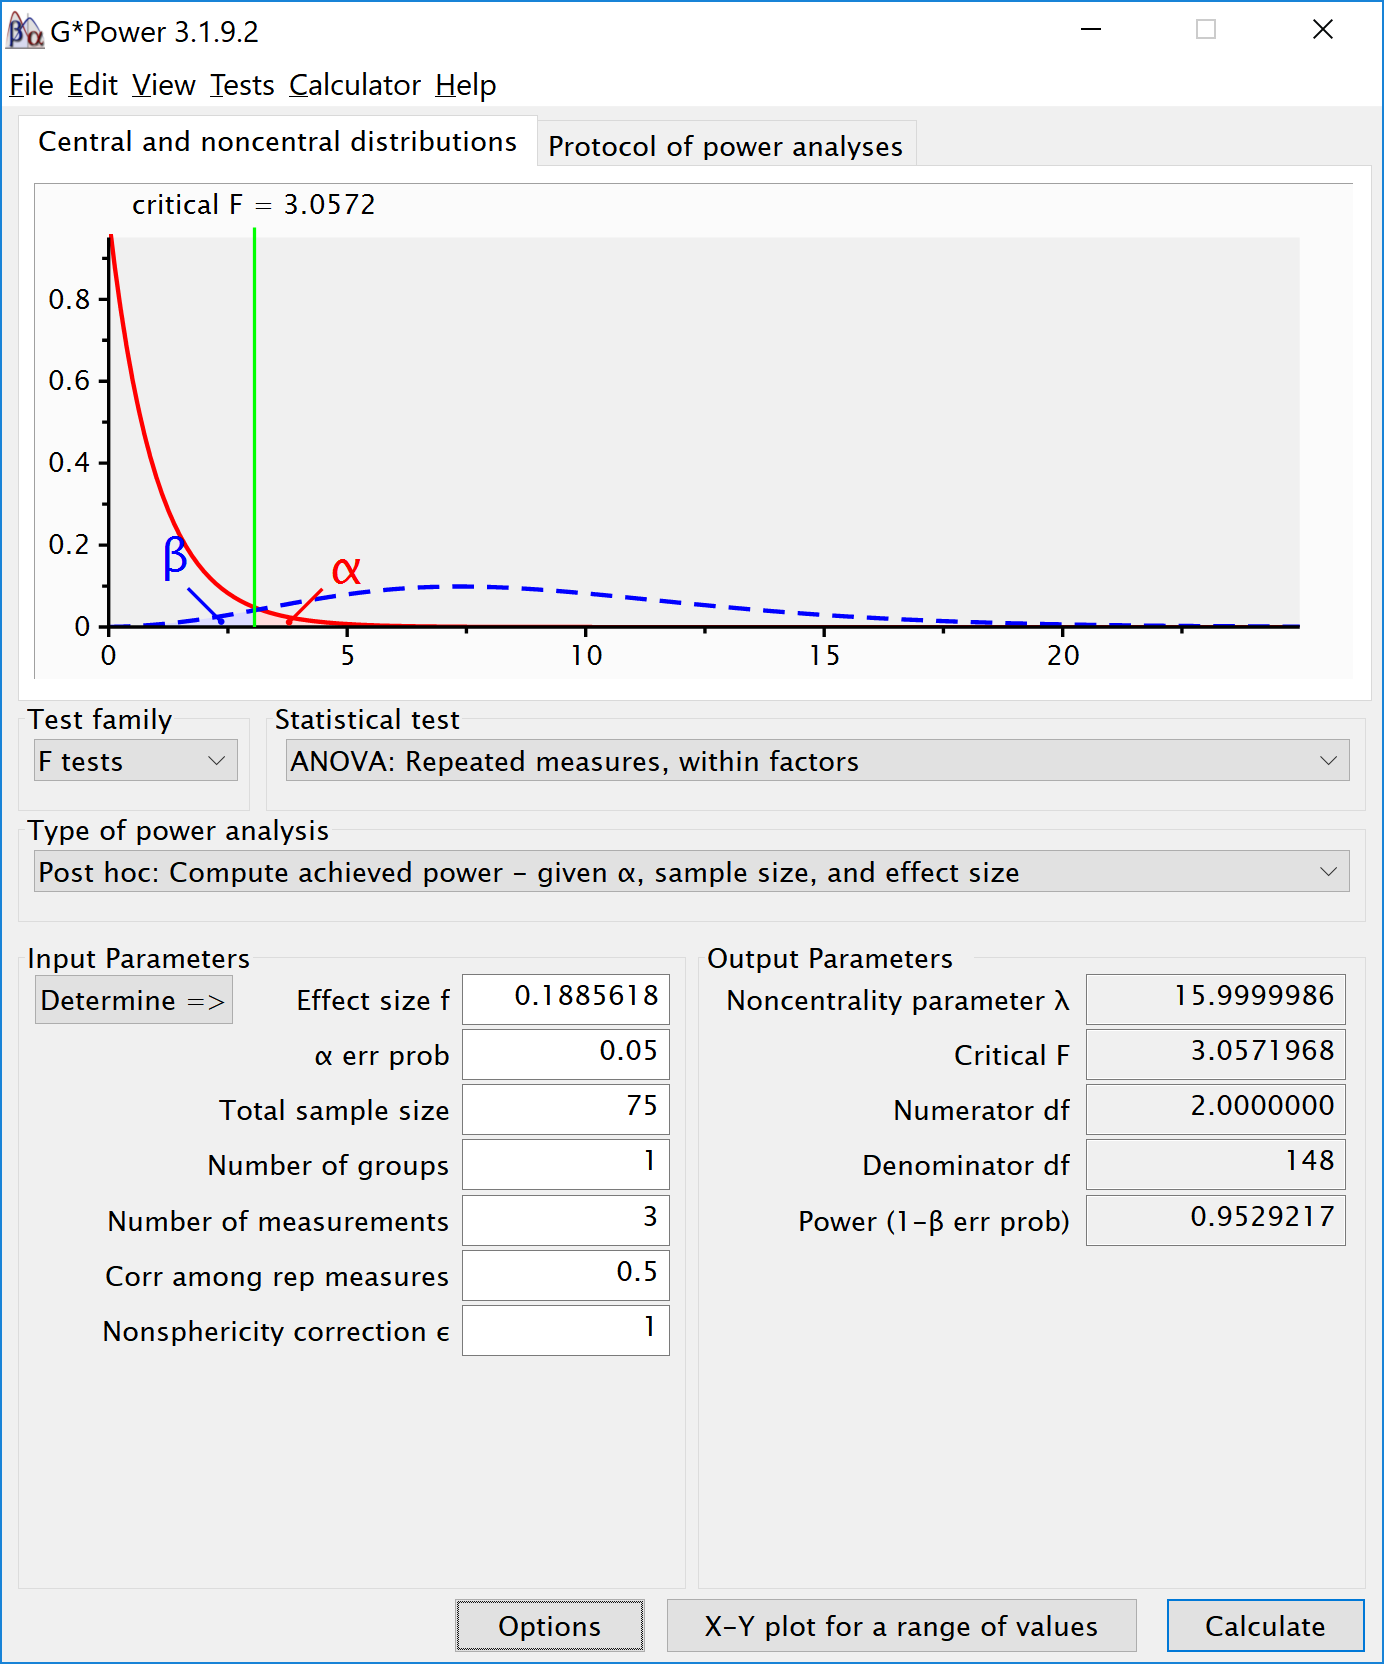
\includegraphics{screenshots/gpower_3.png}

\hypertarget{reproducing-brysbaert-variation-1-changing-correlation}{%
\section{Reproducing Brysbaert Variation 1 Changing Correlation}\label{reproducing-brysbaert-variation-1-changing-correlation}}

\begin{Shaded}
\begin{Highlighting}[]
\CommentTok{# give sample size}
\NormalTok{N =}\StringTok{ }\DecValTok{75}
\CommentTok{# give effect size d}
\NormalTok{d1 =}\StringTok{ }\FloatTok{.4} \CommentTok{#difference between the extremes}
\NormalTok{d2 =}\StringTok{ }\FloatTok{.4} \CommentTok{#third condition goes with the highest extreme}
\CommentTok{# give the correlation between the conditions}
\NormalTok{r =}\StringTok{ }\FloatTok{.6} \CommentTok{#increased correlation}
\CommentTok{# give number of simulations}
\NormalTok{nSim =}\StringTok{ }\NormalTok{nsims}
\CommentTok{# give alpha levels}
\NormalTok{alpha1 =}\StringTok{ }\FloatTok{.05} \CommentTok{#alpha level for the omnibus ANOVA}
\NormalTok{alpha2 =}\StringTok{ }\FloatTok{.05} \CommentTok{#also adjusted from original by DL}
\CommentTok{# create progress bar in case it takes a while}
\CommentTok{#pb <- winProgressBar(title = "progress bar", min = 0, max = nSim, width = 300)}
\CommentTok{# create vectors to store p-values}
\NormalTok{p1 <-}\KeywordTok{numeric}\NormalTok{(nSim) }\CommentTok{#p-value omnibus ANOVA}
\NormalTok{p2 <-}\KeywordTok{numeric}\NormalTok{(nSim) }\CommentTok{#p-value first post hoc test}
\NormalTok{p3 <-}\KeywordTok{numeric}\NormalTok{(nSim) }\CommentTok{#p-value second post hoc test}
\NormalTok{p4 <-}\KeywordTok{numeric}\NormalTok{(nSim) }\CommentTok{#p-value third post hoc test}
\CommentTok{# open library MASS}
\KeywordTok{library}\NormalTok{(}\StringTok{'MASS'}\NormalTok{)}
\CommentTok{# define correlation matrix}
\NormalTok{rho <-}\StringTok{ }\KeywordTok{cbind}\NormalTok{(}\KeywordTok{c}\NormalTok{(}\DecValTok{1}\NormalTok{, r, r), }\KeywordTok{c}\NormalTok{(r, }\DecValTok{1}\NormalTok{, r), }\KeywordTok{c}\NormalTok{(r, r, }\DecValTok{1}\NormalTok{))}
\CommentTok{# define participant codes}
\NormalTok{part <-}\StringTok{ }\KeywordTok{paste}\NormalTok{(}\StringTok{"part"}\NormalTok{,}\KeywordTok{seq}\NormalTok{(}\DecValTok{1}\OperatorTok{:}\NormalTok{N))}
\ControlFlowTok{for}\NormalTok{(i }\ControlFlowTok{in} \DecValTok{1}\OperatorTok{:}\NormalTok{nSim)\{ }\CommentTok{#for each simulated experiment}
 \CommentTok{# setWinProgressBar(pb, i, title=paste(round(i/nSim*100, 1), "% done"))}
\NormalTok{  data =}\StringTok{ }\KeywordTok{mvrnorm}\NormalTok{(}\DataTypeTok{n=}\NormalTok{N, }\DataTypeTok{mu=}\KeywordTok{c}\NormalTok{(}\DecValTok{0}\NormalTok{, }\DecValTok{0}\NormalTok{, }\DecValTok{0}\NormalTok{), }\DataTypeTok{Sigma=}\NormalTok{rho)}
\NormalTok{  data[,}\DecValTok{2}\NormalTok{] =}\StringTok{ }\NormalTok{data[,}\DecValTok{2}\NormalTok{]}\OperatorTok{+}\NormalTok{d1}
\NormalTok{  data[,}\DecValTok{3}\NormalTok{] =}\StringTok{ }\NormalTok{data[,}\DecValTok{3}\NormalTok{]}\OperatorTok{+}\NormalTok{d2}
\NormalTok{  datalong =}\StringTok{ }\KeywordTok{c}\NormalTok{(data[,}\DecValTok{1}\NormalTok{],data[,}\DecValTok{2}\NormalTok{],data[,}\DecValTok{3}\NormalTok{])}
\NormalTok{  conds=}\StringTok{ }\KeywordTok{factor}\NormalTok{(}\KeywordTok{rep}\NormalTok{(letters[}\DecValTok{24}\OperatorTok{:}\DecValTok{26}\NormalTok{], }\DataTypeTok{each =}\NormalTok{ N))}
\NormalTok{  partID =}\StringTok{ }\KeywordTok{factor}\NormalTok{(}\KeywordTok{rep}\NormalTok{(part, }\DataTypeTok{times =} \DecValTok{3}\NormalTok{))}
\NormalTok{  output <-}\KeywordTok{data.frame}\NormalTok{(partID,conds,datalong)}
\NormalTok{  test <-}\StringTok{ }\KeywordTok{aov}\NormalTok{(datalong}\OperatorTok{~}\NormalTok{conds }\OperatorTok{+}\StringTok{ }\KeywordTok{Error}\NormalTok{(partID}\OperatorTok{/}\NormalTok{conds), }\DataTypeTok{data=}\NormalTok{output)}
\NormalTok{  tests <-}\StringTok{ }\NormalTok{(}\KeywordTok{summary}\NormalTok{(test))}
\NormalTok{  p1[i] <-}\StringTok{ }\NormalTok{tests}\OperatorTok{$}\StringTok{'Error: partID:conds'}\NormalTok{[[}\DecValTok{1}\NormalTok{]]}\OperatorTok{$}\StringTok{'Pr(>F)'}\NormalTok{[[}\DecValTok{1}\NormalTok{]]}
\NormalTok{  p2[i] <-}\StringTok{ }\KeywordTok{t.test}\NormalTok{(data[,}\DecValTok{1}\NormalTok{],data[,}\DecValTok{2}\NormalTok{], }\DataTypeTok{paired=}\OtherTok{TRUE}\NormalTok{)}\OperatorTok{$}\NormalTok{p.value}
\NormalTok{  p3[i] <-}\StringTok{ }\KeywordTok{t.test}\NormalTok{(data[,}\DecValTok{1}\NormalTok{],data[,}\DecValTok{3}\NormalTok{], }\DataTypeTok{paired=}\OtherTok{TRUE}\NormalTok{)}\OperatorTok{$}\NormalTok{p.value}
\NormalTok{  p4[i] <-}\StringTok{ }\KeywordTok{t.test}\NormalTok{(data[,}\DecValTok{2}\NormalTok{],data[,}\DecValTok{3}\NormalTok{], }\DataTypeTok{paired=}\OtherTok{TRUE}\NormalTok{)}\OperatorTok{$}\NormalTok{p.value}
\NormalTok{  \}}
\CommentTok{#close(pb)#close progress bar}
\CommentTok{#printing all unique tests (adjusted code by DL)}
\KeywordTok{sum}\NormalTok{(p1}\OperatorTok{<}\NormalTok{alpha1)}\OperatorTok{/}\NormalTok{nSim}
\end{Highlighting}
\end{Shaded}

\begin{verbatim}
## [1] 0.94
\end{verbatim}

\begin{Shaded}
\begin{Highlighting}[]
\KeywordTok{sum}\NormalTok{(p2}\OperatorTok{<}\NormalTok{alpha2)}\OperatorTok{/}\NormalTok{nSim}
\end{Highlighting}
\end{Shaded}

\begin{verbatim}
## [1] 0.93
\end{verbatim}

\begin{Shaded}
\begin{Highlighting}[]
\KeywordTok{sum}\NormalTok{(p3}\OperatorTok{<}\NormalTok{alpha2)}\OperatorTok{/}\NormalTok{nSim}
\end{Highlighting}
\end{Shaded}

\begin{verbatim}
## [1] 0.92
\end{verbatim}

\begin{Shaded}
\begin{Highlighting}[]
\KeywordTok{sum}\NormalTok{(p4}\OperatorTok{<}\NormalTok{alpha2)}\OperatorTok{/}\NormalTok{nSim}
\end{Highlighting}
\end{Shaded}

\begin{verbatim}
## [1] 0.01
\end{verbatim}

\begin{Shaded}
\begin{Highlighting}[]
\NormalTok{design <-}\StringTok{ "3w"}
\NormalTok{n <-}\StringTok{ }\DecValTok{75}
\NormalTok{mu <-}\StringTok{ }\KeywordTok{c}\NormalTok{(}\DecValTok{0}\NormalTok{, }\FloatTok{0.4}\NormalTok{, }\FloatTok{0.4}\NormalTok{)}
\NormalTok{sd <-}\StringTok{ }\DecValTok{1}
\NormalTok{r <-}\StringTok{ }\FloatTok{0.6}
\NormalTok{labelnames <-}\StringTok{ }\KeywordTok{c}\NormalTok{(}\StringTok{"speed"}\NormalTok{, }\StringTok{"fast"}\NormalTok{, }\StringTok{"medium"}\NormalTok{, }\StringTok{"slow"}\NormalTok{)}
\end{Highlighting}
\end{Shaded}

We create the within design, and run the simulation

\begin{Shaded}
\begin{Highlighting}[]
\NormalTok{design_result <-}\StringTok{ }\KeywordTok{ANOVA_design}\NormalTok{(}\DataTypeTok{design =}\NormalTok{ design,}
                   \DataTypeTok{n =}\NormalTok{ n, }
                   \DataTypeTok{mu =}\NormalTok{ mu, }
                   \DataTypeTok{sd =}\NormalTok{ sd, }
                   \DataTypeTok{r =}\NormalTok{ r, }
                   \DataTypeTok{labelnames =}\NormalTok{ labelnames)}
\end{Highlighting}
\end{Shaded}

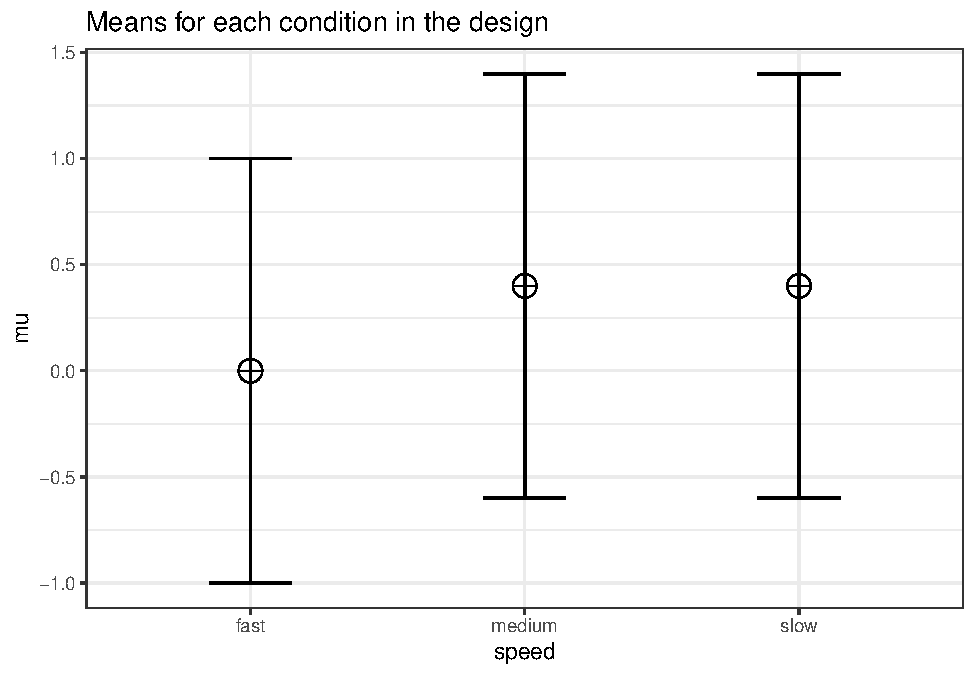
\includegraphics{SuperpowerValidation_files/figure-latex/unnamed-chunk-46-1.pdf}

\begin{Shaded}
\begin{Highlighting}[]
\KeywordTok{ANOVA_power}\NormalTok{(design_result, }\DataTypeTok{nsims =}\NormalTok{ nsims)}
\end{Highlighting}
\end{Shaded}

\begin{verbatim}
## Power and Effect sizes for ANOVA tests
##             power effect_size
## anova_speed    99      0.1223
## 
## Power and Effect sizes for contrasts
##                           power effect_size
## p_speed_fast_speed_medium    98    0.436167
## p_speed_fast_speed_slow      97    0.443268
## p_speed_medium_speed_slow     8   -0.001819
## 
## Within-Subject Factors Included: Check MANOVA Results
\end{verbatim}

Again, this is similar to g*power for the ANOVA:

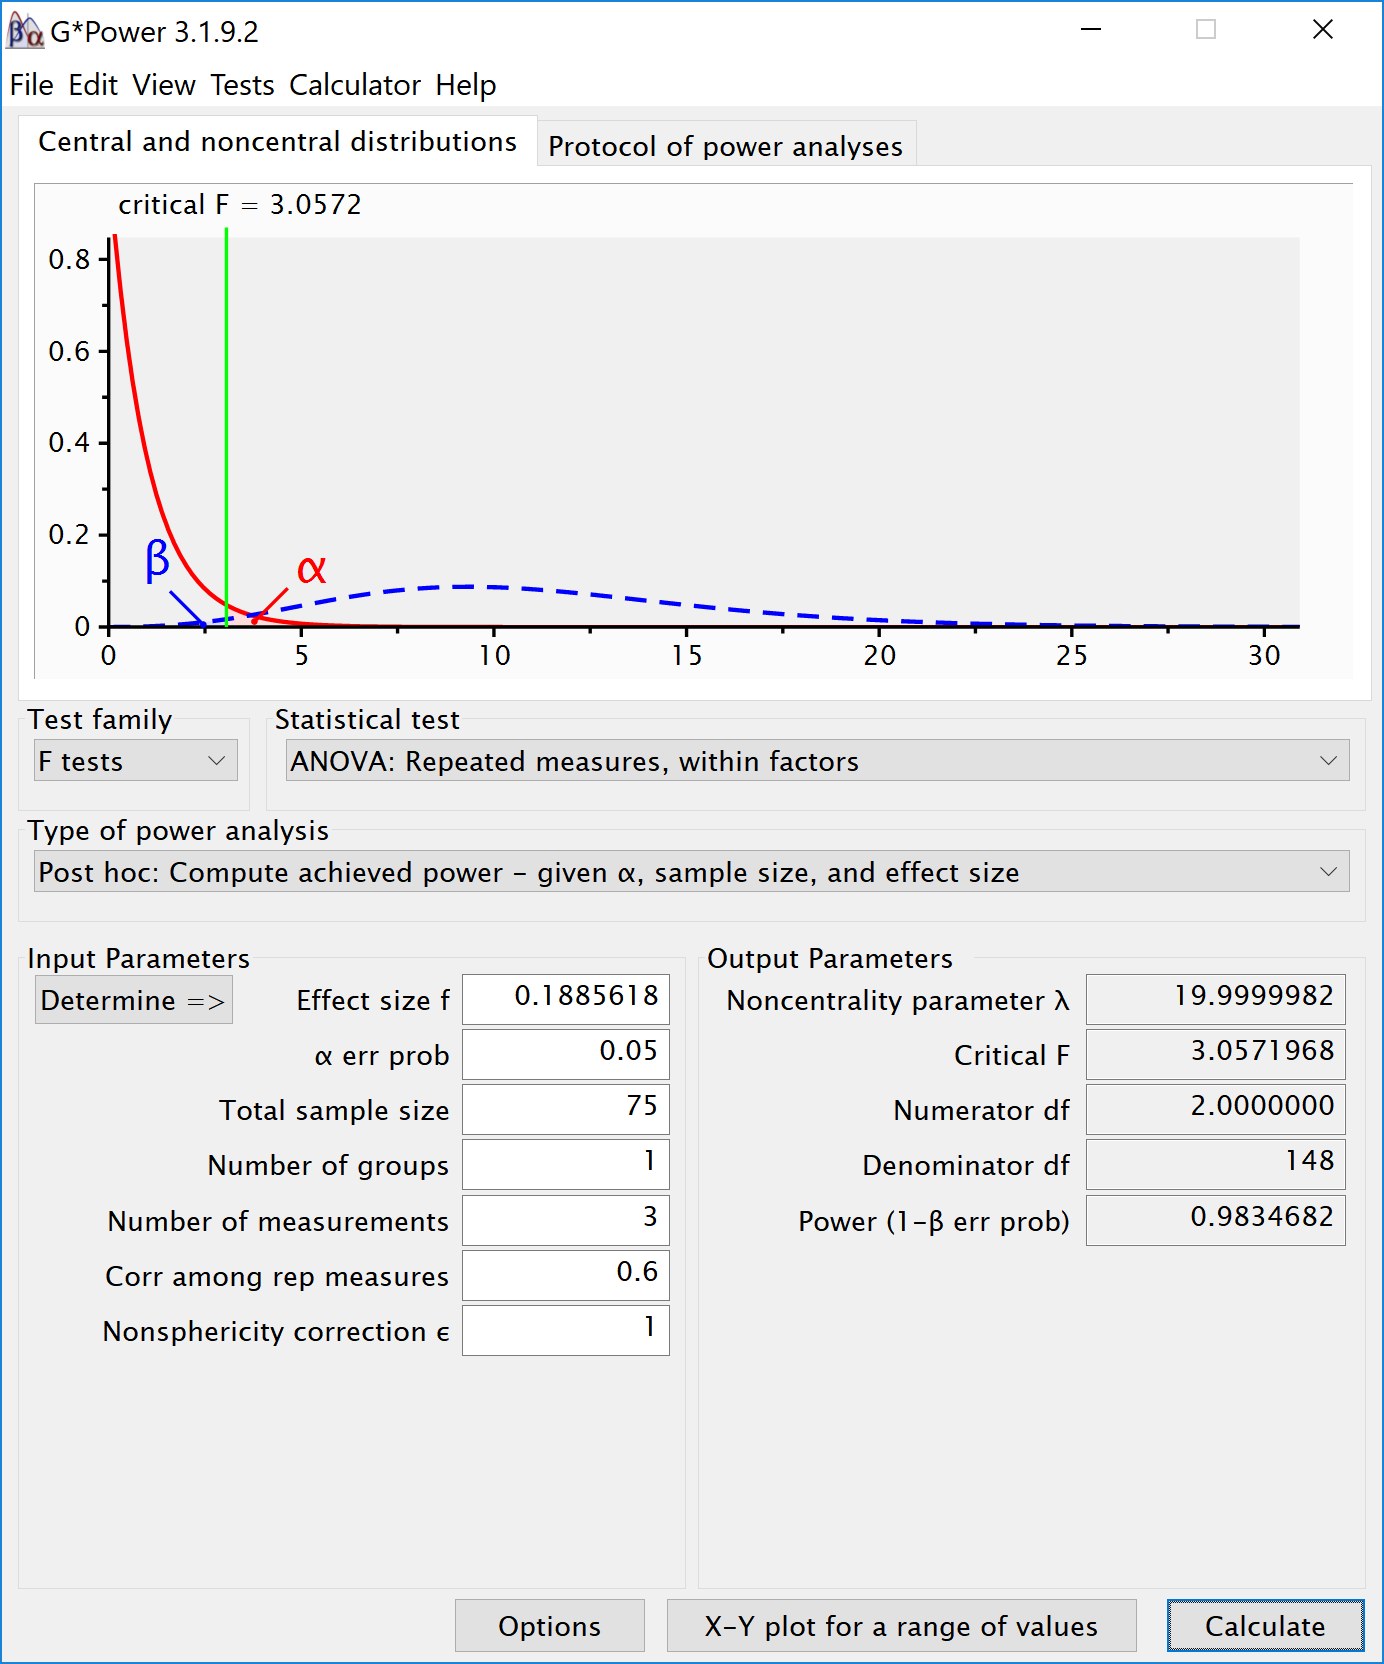
\includegraphics{screenshots/gpower_4.png}

\hypertarget{mixed-anova-part-1}{%
\chapter{Mixed ANOVA Part 1}\label{mixed-anova-part-1}}

\hypertarget{two-by-two-anova-within-between-design}{%
\section{Two by two ANOVA, within-between design}\label{two-by-two-anova-within-between-design}}

We can simulate a Two-Way ANOVA with a specific alpha, sample size and effect size, to achieve a specified statistical power. We wil try to reproduce the power analysis by g*power for an F-test, ANOVA: Repeated measures, within-between interaction.

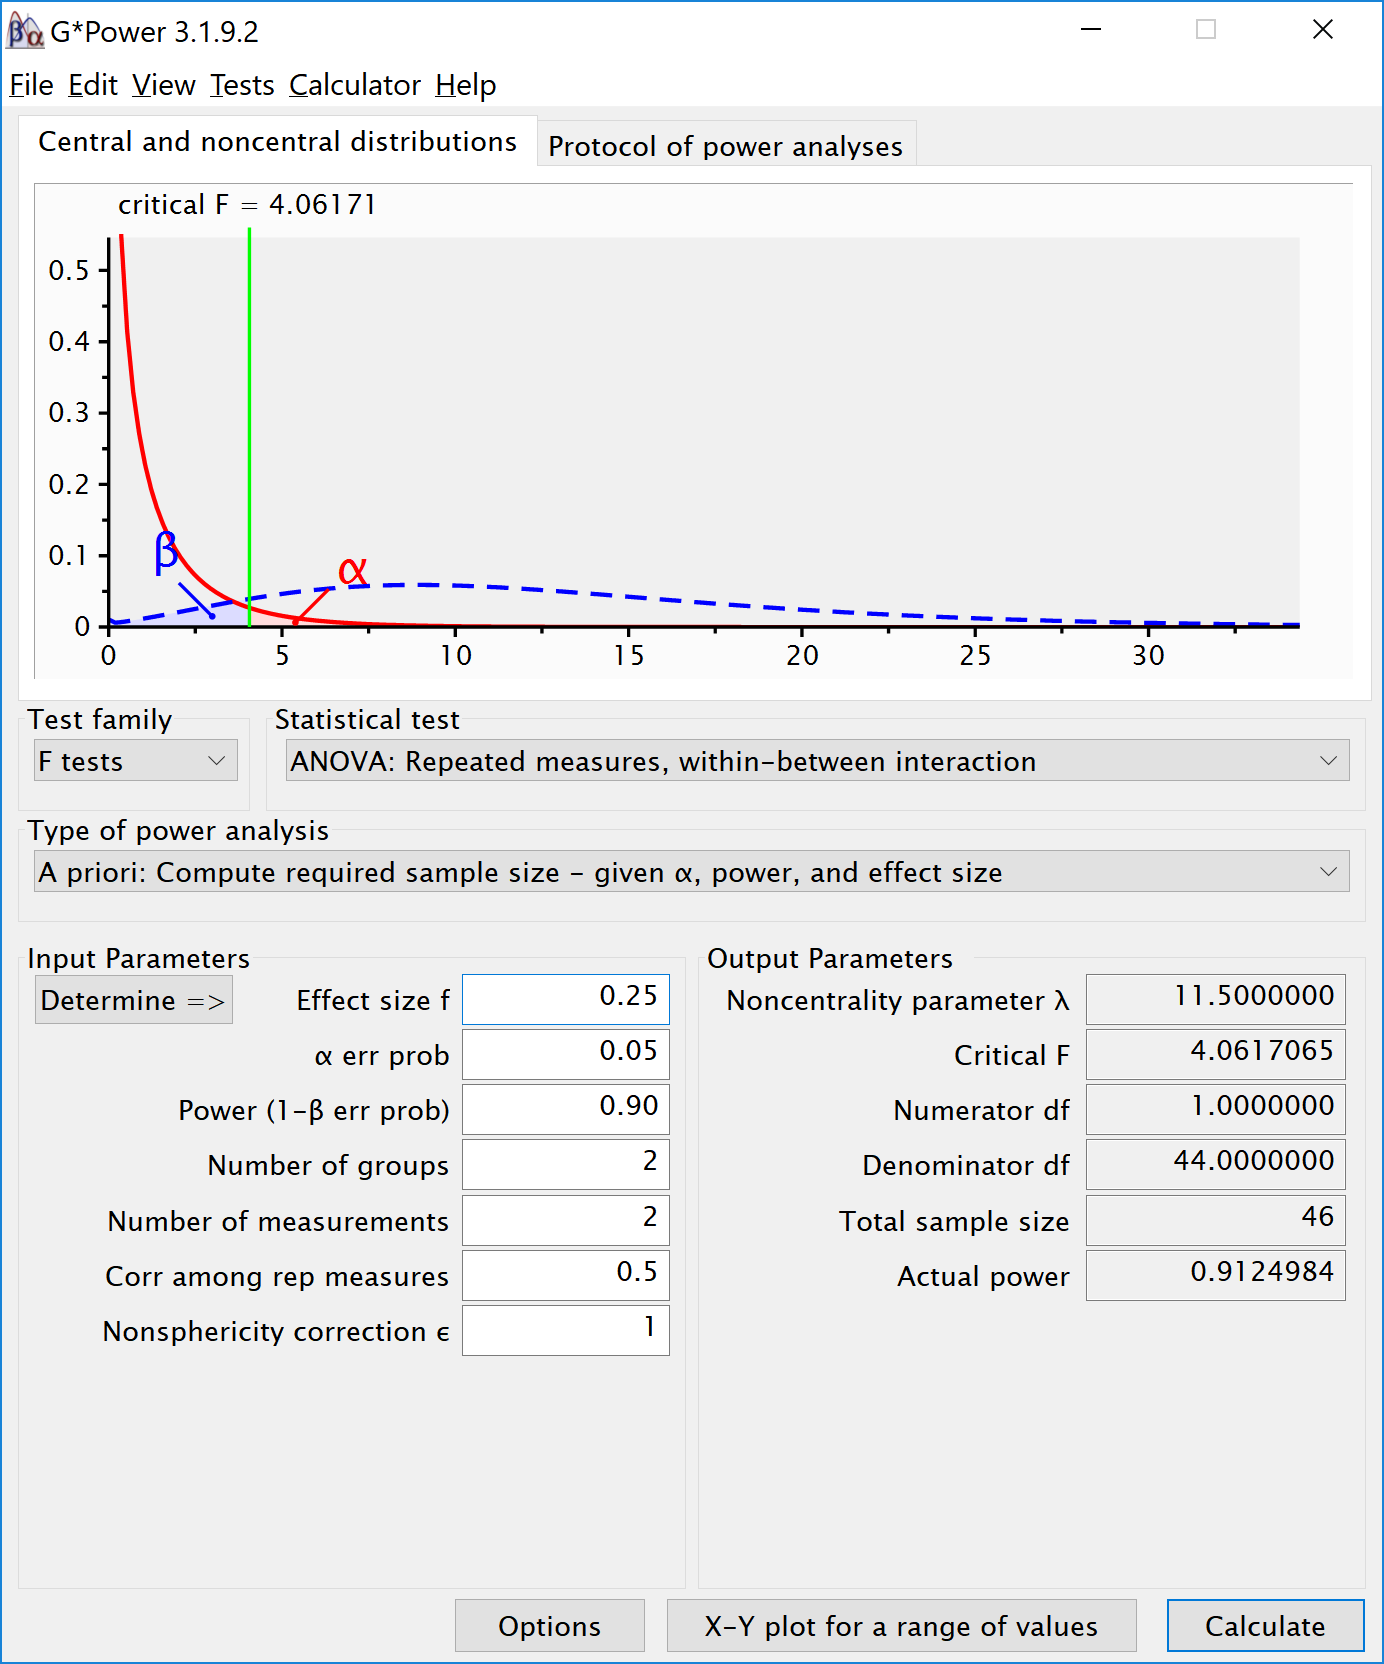
\includegraphics{screenshots/gpower_5.png}

For the 2-way interaction, the result should be a power of 91.25\% is we have a total samplesize of 46. Since we have 2 groups in the between factor that means the sample size per group is 2 (and both these groups collect 2 repeated measures).

\begin{Shaded}
\begin{Highlighting}[]
\NormalTok{mu <-}\StringTok{ }\KeywordTok{c}\NormalTok{(}\OperatorTok{-}\FloatTok{0.25}\NormalTok{, }\FloatTok{0.25}\NormalTok{, }\FloatTok{0.25}\NormalTok{, }\FloatTok{-0.25}\NormalTok{)}
\NormalTok{n <-}\StringTok{ }\DecValTok{23}
\NormalTok{sd <-}\StringTok{ }\DecValTok{1}
\NormalTok{r <-}\StringTok{ }\FloatTok{0.5}
\NormalTok{string =}\StringTok{ "2w*2b"}
\NormalTok{alpha_level <-}\StringTok{ }\FloatTok{0.05}
\NormalTok{labelnames =}\StringTok{ }\KeywordTok{c}\NormalTok{(}\StringTok{"age"}\NormalTok{, }\StringTok{"old"}\NormalTok{, }\StringTok{"young"}\NormalTok{, }\StringTok{"color"}\NormalTok{, }\StringTok{"blue"}\NormalTok{, }\StringTok{"red"}\NormalTok{)}
\NormalTok{design_result <-}\StringTok{ }\KeywordTok{ANOVA_design}\NormalTok{(}\DataTypeTok{design =}\NormalTok{ string,}
                              \DataTypeTok{n =}\NormalTok{ n, }
                              \DataTypeTok{mu =}\NormalTok{ mu, }
                              \DataTypeTok{sd =}\NormalTok{ sd, }
                              \DataTypeTok{r =}\NormalTok{ r, }
                              \DataTypeTok{labelnames =}\NormalTok{ labelnames)}
\end{Highlighting}
\end{Shaded}

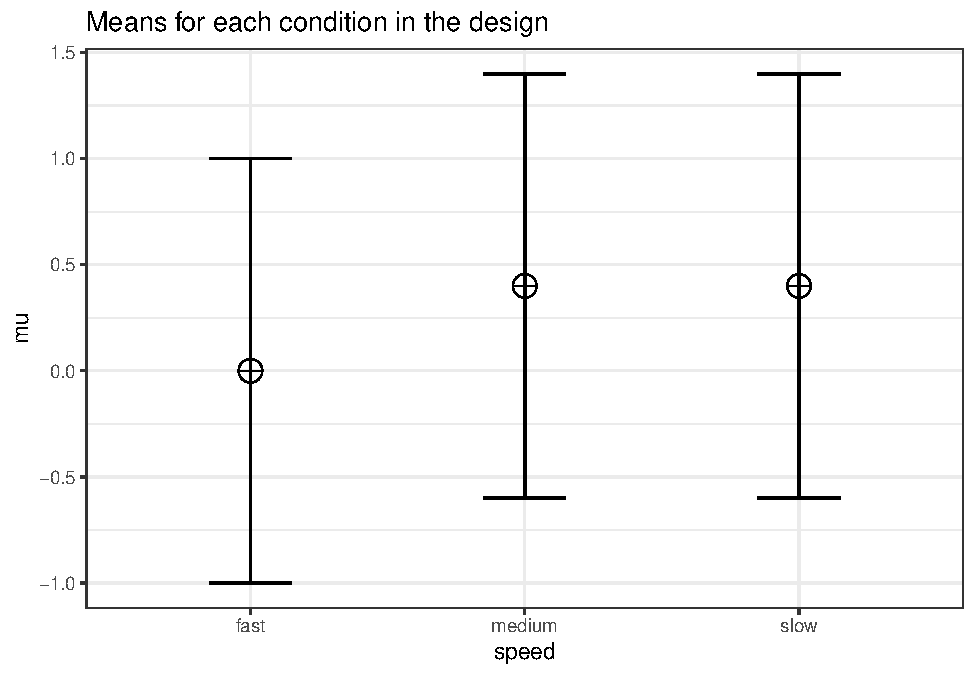
\includegraphics{SuperpowerValidation_files/figure-latex/unnamed-chunk-47-1.pdf}

\begin{Shaded}
\begin{Highlighting}[]
\NormalTok{simulation_result <-}\StringTok{ }\KeywordTok{ANOVA_power}\NormalTok{(design_result, }\DataTypeTok{alpha =} \FloatTok{0.05}\NormalTok{, }\DataTypeTok{nsims =}\NormalTok{ nsims)}
\end{Highlighting}
\end{Shaded}

\begin{verbatim}
## Power and Effect sizes for ANOVA tests
##                 power effect_size
## anova_color         5     0.02118
## anova_age           6     0.02362
## anova_color:age    91     0.20318
## 
## Power and Effect sizes for contrasts
##                                            power effect_size
## p_age_old_color_blue_age_old_color_red        28     0.46087
## p_age_old_color_blue_age_young_color_blue     56     0.49235
## p_age_old_color_blue_age_young_color_red       9    -0.02785
## p_age_old_color_red_age_young_color_blue       5     0.01655
## p_age_old_color_red_age_young_color_red       59    -0.50668
## p_age_young_color_blue_age_young_color_red    37    -0.50244
## 
## Within-Subject Factors Included: Check MANOVA Results
\end{verbatim}

\hypertarget{two-by-two-anova-within-between-design-variation-1}{%
\section{Two by two ANOVA, within-between design Variation 1}\label{two-by-two-anova-within-between-design-variation-1}}

We can simulate the same Two-Way ANOVA increasing the correlation to 0.7.

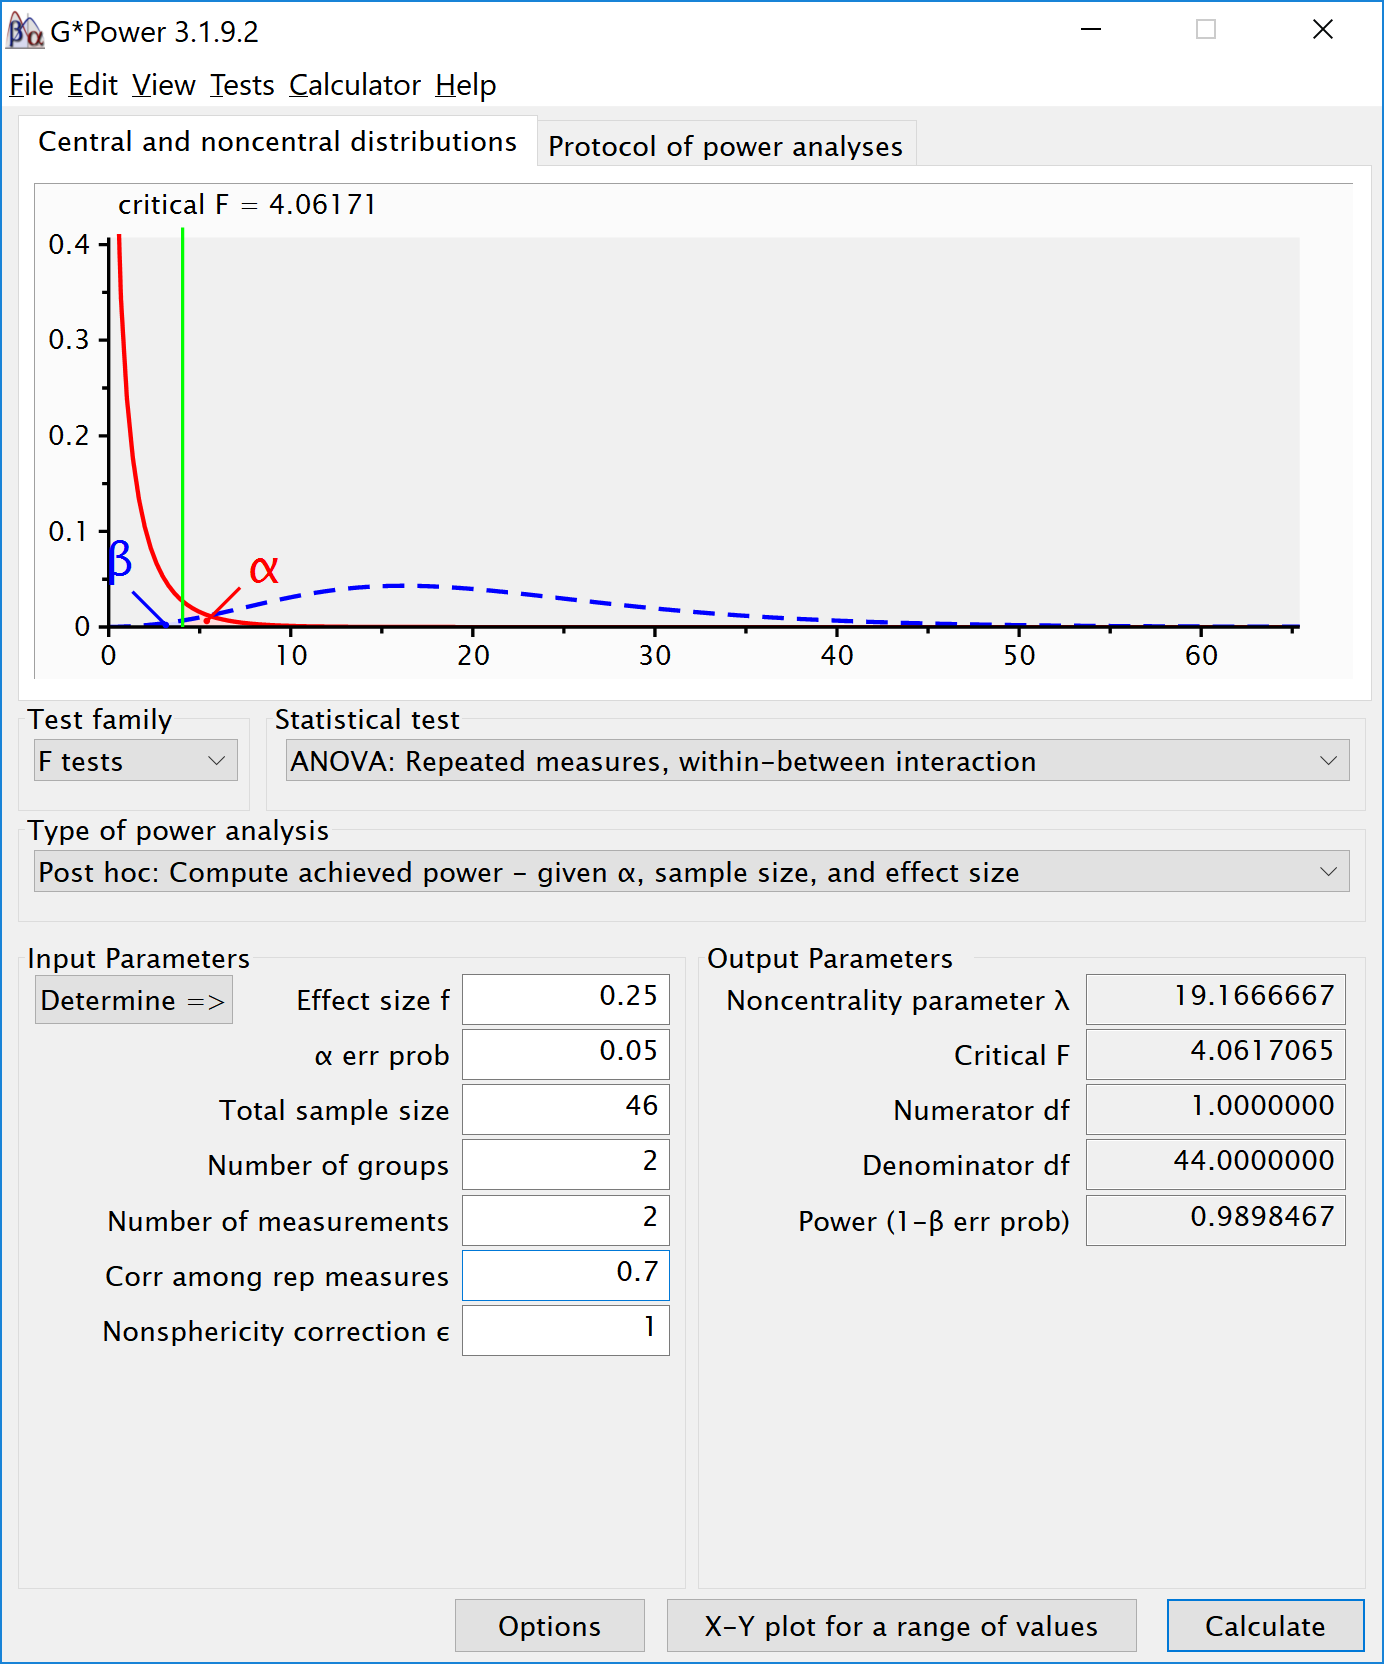
\includegraphics{screenshots/gpower_6.png}

\begin{Shaded}
\begin{Highlighting}[]
\NormalTok{mu <-}\StringTok{ }\KeywordTok{c}\NormalTok{(}\OperatorTok{-}\FloatTok{0.25}\NormalTok{, }\FloatTok{0.25}\NormalTok{, }\FloatTok{0.25}\NormalTok{, }\FloatTok{-0.25}\NormalTok{)}
\NormalTok{n <-}\StringTok{ }\DecValTok{23}
\NormalTok{sd <-}\StringTok{ }\DecValTok{1}
\NormalTok{r <-}\StringTok{ }\FloatTok{0.7}
\NormalTok{string =}\StringTok{ "2w*2b"}
\NormalTok{alpha_level <-}\StringTok{ }\FloatTok{0.05}
\NormalTok{labelnames =}\StringTok{ }\KeywordTok{c}\NormalTok{(}\StringTok{"age"}\NormalTok{, }\StringTok{"old"}\NormalTok{, }\StringTok{"young"}\NormalTok{, }\StringTok{"color"}\NormalTok{, }\StringTok{"blue"}\NormalTok{, }\StringTok{"red"}\NormalTok{)}
\NormalTok{design_result <-}\StringTok{ }\KeywordTok{ANOVA_design}\NormalTok{(}\DataTypeTok{design =}\NormalTok{ string,}
                              \DataTypeTok{n =}\NormalTok{ n, }
                              \DataTypeTok{mu =}\NormalTok{ mu, }
                              \DataTypeTok{sd =}\NormalTok{ sd, }
                              \DataTypeTok{r =}\NormalTok{ r, }
                              \DataTypeTok{labelnames =}\NormalTok{ labelnames)}
\end{Highlighting}
\end{Shaded}

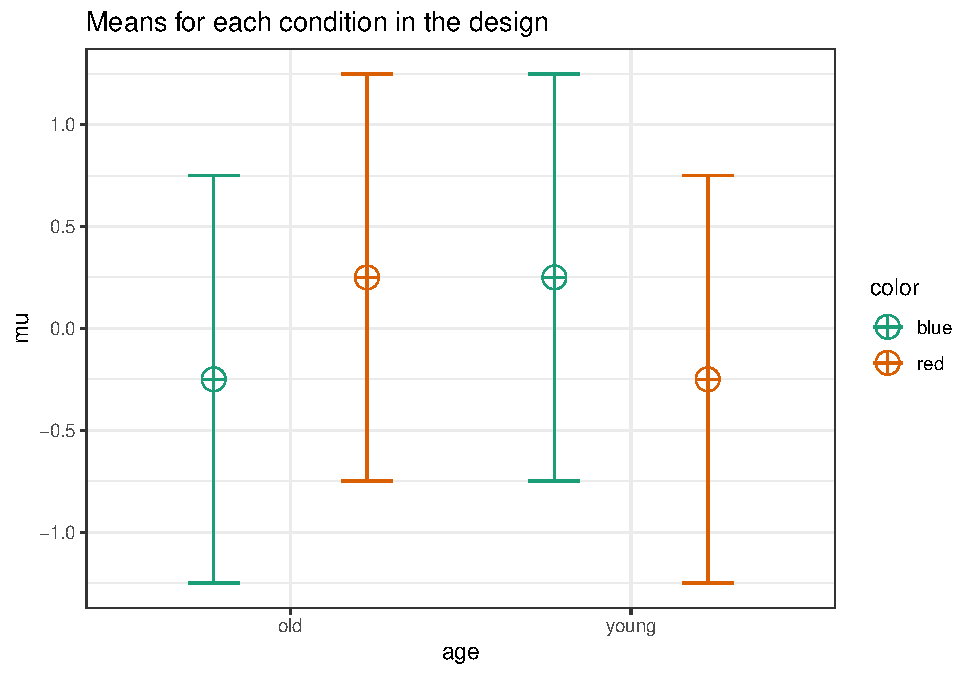
\includegraphics{SuperpowerValidation_files/figure-latex/unnamed-chunk-48-1.pdf}

\begin{Shaded}
\begin{Highlighting}[]
\NormalTok{simulation_result <-}\StringTok{ }\KeywordTok{ANOVA_power}\NormalTok{(design_result, }\DataTypeTok{alpha =} \FloatTok{0.05}\NormalTok{, }\DataTypeTok{nsims =}\NormalTok{ nsims)}
\end{Highlighting}
\end{Shaded}

\begin{verbatim}
## Power and Effect sizes for ANOVA tests
##                 power effect_size
## anova_color         2     0.01759
## anova_age           7     0.02260
## anova_color:age    98     0.29823
## 
## Power and Effect sizes for contrasts
##                                            power effect_size
## p_age_old_color_blue_age_old_color_red        45     0.54169
## p_age_old_color_blue_age_young_color_blue     87     0.68826
## p_age_old_color_blue_age_young_color_red       5     0.04402
## p_age_old_color_red_age_young_color_blue       2    -0.01272
## p_age_old_color_red_age_young_color_red       77    -0.62245
## p_age_young_color_blue_age_young_color_red    34    -0.47829
## 
## Within-Subject Factors Included: Check MANOVA Results
\end{verbatim}

\hypertarget{mixed-anova-part-2}{%
\chapter{Mixed ANOVA Part 2}\label{mixed-anova-part-2}}

\hypertarget{two-by-two-anova-within-within-design}{%
\section{Two by two ANOVA, within-within design}\label{two-by-two-anova-within-within-design}}

We can simulate a 2x2 ANOVA, both factors manipulated within participants, with a specific sample size and effect size, to achieve a desired statistical power.

As Potvin \& Schutz (2000) explain, analytic procedures for a two-factor repeated measures ANOVA do not seem to exist. The main problem is quantifying the error variance (the denominator when calculating lambda or Cohen's f). Simulation based aproaches provide a solution.

We can reproduce the simulation coded by \href{https://cognitivedatascientist.com/2015/12/14/power-simulation-in-r-the-repeated-measures-anova-5/}{Ben Amsel}

\begin{Shaded}
\begin{Highlighting}[]
\NormalTok{knitr}\OperatorTok{::}\NormalTok{opts_chunk}\OperatorTok{$}\KeywordTok{set}\NormalTok{(}\DataTypeTok{echo=}\OtherTok{TRUE}\NormalTok{, }\DataTypeTok{warning=}\OtherTok{FALSE}\NormalTok{, }\DataTypeTok{message=}\OtherTok{FALSE}\NormalTok{)}
 
\CommentTok{# define the parameters}
\NormalTok{mu =}\StringTok{ }\KeywordTok{c}\NormalTok{(}\DecValTok{700}\NormalTok{, }\DecValTok{670}\NormalTok{, }\DecValTok{670}\NormalTok{, }\DecValTok{700}\NormalTok{) }\CommentTok{# true effects (in this case, a double dissociation)}
\NormalTok{sigma =}\StringTok{ }\DecValTok{150}  \CommentTok{# population standard deviation}
\NormalTok{rho =}\StringTok{ }\FloatTok{0.75} \CommentTok{# correlation between repeated measures}
\NormalTok{nsubs =}\StringTok{ }\DecValTok{25} \CommentTok{# how many subjects?}
\NormalTok{nsims =}\StringTok{ }\NormalTok{nsims }\CommentTok{# how many simulation replicates?}
 
\CommentTok{# create 2 factors representing the 2 independent variables}
\NormalTok{cond =}\StringTok{ }\KeywordTok{data.frame}\NormalTok{(}
  \DataTypeTok{X1 =} \KeywordTok{rep}\NormalTok{(}\KeywordTok{factor}\NormalTok{(letters[}\DecValTok{1}\OperatorTok{:}\DecValTok{2}\NormalTok{]), nsubs }\OperatorTok{*}\StringTok{ }\DecValTok{2}\NormalTok{),}
  \DataTypeTok{X2 =} \KeywordTok{rep}\NormalTok{(}\KeywordTok{factor}\NormalTok{(letters[}\DecValTok{1}\OperatorTok{:}\DecValTok{2}\NormalTok{]), nsubs, }\DataTypeTok{each=}\DecValTok{2}\NormalTok{))}
 
\CommentTok{# create a subjects factor}
\NormalTok{subject =}\StringTok{ }\KeywordTok{factor}\NormalTok{(}\KeywordTok{sort}\NormalTok{(}\KeywordTok{rep}\NormalTok{(}\DecValTok{1}\OperatorTok{:}\NormalTok{nsubs, }\DecValTok{4}\NormalTok{)))}
 
\CommentTok{# combine above into the design matrix}
\NormalTok{dm =}\StringTok{ }\KeywordTok{data.frame}\NormalTok{(subject, cond)}
\end{Highlighting}
\end{Shaded}

Build Sigma: the population variance-covariance matrix

\begin{Shaded}
\begin{Highlighting}[]
\CommentTok{# create k x k matrix populated with sigma}
\NormalTok{sigma.mat <-}\StringTok{ }\KeywordTok{rep}\NormalTok{(sigma, }\DecValTok{4}\NormalTok{)}
\NormalTok{S <-}\StringTok{ }\KeywordTok{matrix}\NormalTok{(sigma.mat, }\DataTypeTok{ncol=}\KeywordTok{length}\NormalTok{(sigma.mat), }\DataTypeTok{nrow=}\KeywordTok{length}\NormalTok{(sigma.mat))}
 
\CommentTok{# compute covariance between measures}
\NormalTok{Sigma <-}\StringTok{ }\KeywordTok{t}\NormalTok{(S) }\OperatorTok{*}\StringTok{ }\NormalTok{S }\OperatorTok{*}\StringTok{ }\NormalTok{rho  }
 
\CommentTok{# put the variances on the diagonal }
\KeywordTok{diag}\NormalTok{(Sigma) <-}\StringTok{ }\NormalTok{sigma}\OperatorTok{^}\DecValTok{2}  
\end{Highlighting}
\end{Shaded}

Run the simulation

\begin{Shaded}
\begin{Highlighting}[]
\CommentTok{# stack 'nsims' individual data frames into one large data frame}
\NormalTok{df =}\StringTok{ }\NormalTok{dm[}\KeywordTok{rep}\NormalTok{(}\KeywordTok{seq_len}\NormalTok{(}\KeywordTok{nrow}\NormalTok{(dm)), nsims), ]}
 
\CommentTok{# add an index column to track the simulation run}
\NormalTok{df}\OperatorTok{$}\NormalTok{simID =}\StringTok{ }\KeywordTok{sort}\NormalTok{(}\KeywordTok{rep}\NormalTok{(}\KeywordTok{seq_len}\NormalTok{(nsims), }\KeywordTok{nrow}\NormalTok{(dm)))}
 
\CommentTok{# sample the observed data from a multivariate normal distribution}
\CommentTok{# using MASS::mvrnorm with the parameters mu and Sigma created earlier}
\CommentTok{# and bind to the existing df}
 
\KeywordTok{require}\NormalTok{(MASS)}
\NormalTok{make.y =}\StringTok{ }\KeywordTok{expression}\NormalTok{(}\KeywordTok{as.vector}\NormalTok{(}\KeywordTok{t}\NormalTok{(}\KeywordTok{mvrnorm}\NormalTok{(nsubs, mu, Sigma))))}
\NormalTok{df}\OperatorTok{$}\NormalTok{y =}\StringTok{ }\KeywordTok{as.vector}\NormalTok{(}\KeywordTok{replicate}\NormalTok{(nsims, }\KeywordTok{eval}\NormalTok{(make.y)))             }
 
\CommentTok{# use do(), the general purpose complement to the specialized data }
\CommentTok{# manipulation functions available in dplyr, to run the ANOVA on}
\CommentTok{# each section of the grouped data frame created by group_by}
 
\KeywordTok{require}\NormalTok{(dplyr)}
\KeywordTok{require}\NormalTok{(car)}
\KeywordTok{require}\NormalTok{(broom)}
 
\NormalTok{mods <-}\StringTok{ }\NormalTok{df }\OperatorTok\StringTok{ }
\StringTok{  }\KeywordTok{group_by}\NormalTok{(simID) }\OperatorTok\StringTok{ }
\StringTok{    }\KeywordTok{do}\NormalTok{(}\DataTypeTok{model =} \KeywordTok{aov}\NormalTok{(y }\OperatorTok{~}\StringTok{ }\NormalTok{X1 }\OperatorTok{*}\StringTok{ }\NormalTok{X2 }\OperatorTok{+}\StringTok{ }\KeywordTok{Error}\NormalTok{(subject }\OperatorTok{/}\StringTok{ }\NormalTok{(X1}\OperatorTok{*}\NormalTok{X2)), }\DataTypeTok{qr=}\OtherTok{FALSE}\NormalTok{, }\DataTypeTok{data =}\NormalTok{ .)) }
 
\CommentTok{# extract p-values for each effect and store in a data frame}
\NormalTok{p =}\StringTok{ }\KeywordTok{data.frame}\NormalTok{(}
\NormalTok{  mods }\OperatorTok\StringTok{ }\KeywordTok{do}\NormalTok{(}\KeywordTok{as.data.frame}\NormalTok{(}\KeywordTok{tidy}\NormalTok{(.}\OperatorTok{$}\NormalTok{model[[}\DecValTok{3}\NormalTok{]])}\OperatorTok{$}\NormalTok{p.value[}\DecValTok{1}\NormalTok{])),}
\NormalTok{  mods }\OperatorTok\StringTok{ }\KeywordTok{do}\NormalTok{(}\KeywordTok{as.data.frame}\NormalTok{(}\KeywordTok{tidy}\NormalTok{(.}\OperatorTok{$}\NormalTok{model[[}\DecValTok{4}\NormalTok{]])}\OperatorTok{$}\NormalTok{p.value[}\DecValTok{1}\NormalTok{])),}
\NormalTok{  mods }\OperatorTok\StringTok{ }\KeywordTok{do}\NormalTok{(}\KeywordTok{as.data.frame}\NormalTok{(}\KeywordTok{tidy}\NormalTok{(.}\OperatorTok{$}\NormalTok{model[[}\DecValTok{5}\NormalTok{]])}\OperatorTok{$}\NormalTok{p.value[}\DecValTok{1}\NormalTok{])))}
\KeywordTok{colnames}\NormalTok{(p) =}\StringTok{ }\KeywordTok{c}\NormalTok{(}\StringTok{'X1'}\NormalTok{,}\StringTok{'X2'}\NormalTok{,}\StringTok{'Interaction'}\NormalTok{)}
\end{Highlighting}
\end{Shaded}

The empirical power is easy to compute, it's just the proportion of simulation runs where p \textless. 05.

\begin{Shaded}
\begin{Highlighting}[]
\NormalTok{power.res =}\StringTok{ }\KeywordTok{apply}\NormalTok{(}\KeywordTok{as.matrix}\NormalTok{(p), }\DecValTok{2}\NormalTok{, }
  \ControlFlowTok{function}\NormalTok{(x) }\KeywordTok{round}\NormalTok{(}\KeywordTok{mean}\NormalTok{(}\KeywordTok{ifelse}\NormalTok{(x }\OperatorTok{<}\StringTok{ }\FloatTok{.05}\NormalTok{, }\DecValTok{1}\NormalTok{, }\DecValTok{0}\NormalTok{) }\OperatorTok{*}\StringTok{ }\DecValTok{100}\NormalTok{),}\DecValTok{2}\NormalTok{))}
\NormalTok{power.res}
\end{Highlighting}
\end{Shaded}

\begin{verbatim}
##          X1          X2 Interaction 
##           3           6          47
\end{verbatim}

Visualize the distributions of p-values

\begin{Shaded}
\begin{Highlighting}[]
\CommentTok{# plot the known effects}
\KeywordTok{require}\NormalTok{(ggplot2)}
\KeywordTok{require}\NormalTok{(gridExtra)}
 
\NormalTok{means =}\StringTok{ }\KeywordTok{data.frame}\NormalTok{(cond[}\DecValTok{1}\OperatorTok{:}\DecValTok{4}\NormalTok{, ], mu, }\DataTypeTok{SE =}\NormalTok{ sigma }\OperatorTok{/}\StringTok{ }\KeywordTok{sqrt}\NormalTok{(nsubs))}
\NormalTok{plt1 =}\StringTok{ }\KeywordTok{ggplot}\NormalTok{(means, }\KeywordTok{aes}\NormalTok{(}\DataTypeTok{y =}\NormalTok{ mu, }\DataTypeTok{x =}\NormalTok{ X1, }\DataTypeTok{fill=}\NormalTok{X2)) }\OperatorTok{+}
\StringTok{  }\KeywordTok{geom_bar}\NormalTok{(}\DataTypeTok{position =} \KeywordTok{position_dodge}\NormalTok{(), }\DataTypeTok{stat=}\StringTok{"identity"}\NormalTok{) }\OperatorTok{+}
\StringTok{  }\KeywordTok{geom_errorbar}\NormalTok{(}\KeywordTok{aes}\NormalTok{(}\DataTypeTok{ymin =}\NormalTok{ mu}\OperatorTok{-}\NormalTok{SE, }\DataTypeTok{ymax =}\NormalTok{ mu}\OperatorTok{+}\NormalTok{SE), }
    \DataTypeTok{position =} \KeywordTok{position_dodge}\NormalTok{(}\DataTypeTok{width=}\FloatTok{0.9}\NormalTok{), }\DataTypeTok{size=}\NormalTok{.}\DecValTok{6}\NormalTok{, }\DataTypeTok{width=}\NormalTok{.}\DecValTok{3}\NormalTok{) }\OperatorTok{+}
\StringTok{  }\KeywordTok{coord_cartesian}\NormalTok{(}\DataTypeTok{ylim=}\KeywordTok{c}\NormalTok{((.}\DecValTok{7}\OperatorTok{*}\KeywordTok{min}\NormalTok{(mu)), }\FloatTok{1.2}\OperatorTok{*}\KeywordTok{max}\NormalTok{(mu))) }\OperatorTok{+}
\StringTok{  }\KeywordTok{theme_bw}\NormalTok{()}
 
\CommentTok{# melt the data into a ggplot friendly 'long' format}
\KeywordTok{require}\NormalTok{(reshape2)}
\NormalTok{plotData <-}\StringTok{ }\KeywordTok{melt}\NormalTok{(p, }\DataTypeTok{value.name =} \StringTok{'p'}\NormalTok{)}
 
\CommentTok{# plot each of the p-value distributions on a log scale}
\KeywordTok{options}\NormalTok{(}\DataTypeTok{scipen =} \DecValTok{999}\NormalTok{) }\CommentTok{# 'turn off' scientific notation}
\NormalTok{plt2 =}\StringTok{ }\KeywordTok{ggplot}\NormalTok{(plotData, }\KeywordTok{aes}\NormalTok{(}\DataTypeTok{x =}\NormalTok{ p)) }\OperatorTok{+}
\StringTok{    }\KeywordTok{scale_x_log10}\NormalTok{(}\DataTypeTok{breaks=}\KeywordTok{c}\NormalTok{(}\DecValTok{1}\NormalTok{, }\FloatTok{0.05}\NormalTok{, }\FloatTok{0.001}\NormalTok{), }
                  \DataTypeTok{labels=}\KeywordTok{c}\NormalTok{(}\DecValTok{1}\NormalTok{, }\FloatTok{0.05}\NormalTok{, }\FloatTok{0.001}\NormalTok{)) }\OperatorTok{+}
\StringTok{    }\KeywordTok{geom_histogram}\NormalTok{(}\DataTypeTok{colour =} \StringTok{"darkblue"}\NormalTok{, }\DataTypeTok{fill =} \StringTok{"white"}\NormalTok{) }\OperatorTok{+}
\StringTok{    }\KeywordTok{geom_vline}\NormalTok{(}\DataTypeTok{xintercept =} \FloatTok{0.05}\NormalTok{, }\DataTypeTok{colour=}\StringTok{'red'}\NormalTok{) }\OperatorTok{+}
\StringTok{    }\KeywordTok{facet_grid}\NormalTok{(variable }\OperatorTok{~}\StringTok{ }\NormalTok{.) }\OperatorTok{+}
\StringTok{    }\KeywordTok{labs}\NormalTok{(}\DataTypeTok{x =} \KeywordTok{expression}\NormalTok{(Log[}\DecValTok{10}\NormalTok{]}\OperatorTok{~}\NormalTok{P)) }\OperatorTok{+}
\StringTok{    }\KeywordTok{theme}\NormalTok{(}\DataTypeTok{axis.text.x =} \KeywordTok{element_text}\NormalTok{(}\DataTypeTok{color=}\StringTok{'black'}\NormalTok{, }\DataTypeTok{size=}\DecValTok{7}\NormalTok{))}
 
\CommentTok{# arrange plots side by side and print}
\KeywordTok{grid.arrange}\NormalTok{(plt1, plt2, }\DataTypeTok{nrow=}\DecValTok{1}\NormalTok{)}
\end{Highlighting}
\end{Shaded}

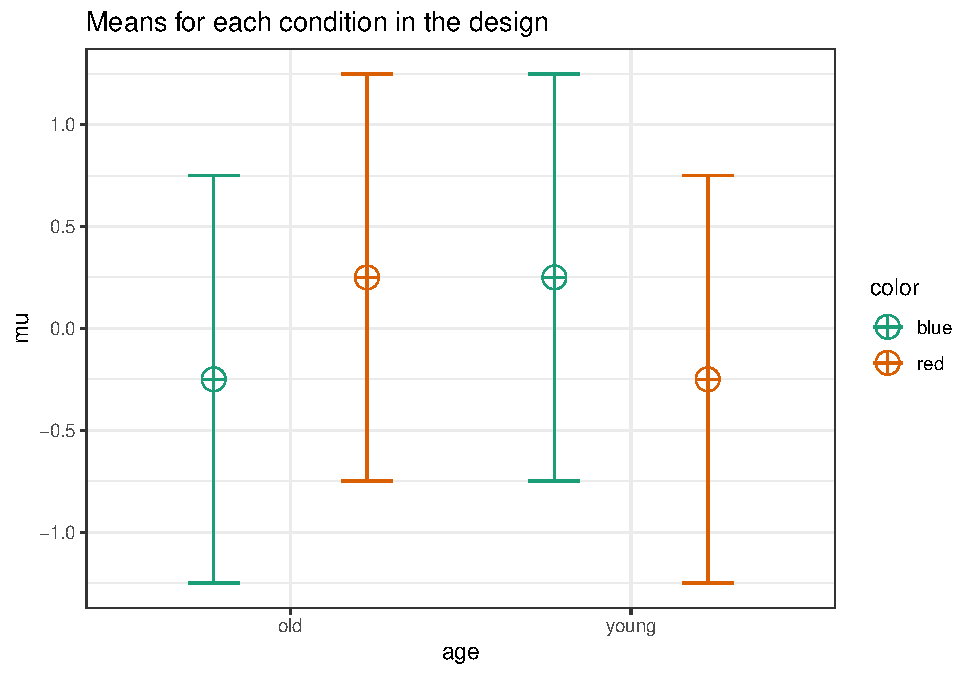
\includegraphics{SuperpowerValidation_files/figure-latex/unnamed-chunk-53-1.pdf}

We can reproduce this simulation:

\begin{Shaded}
\begin{Highlighting}[]
\NormalTok{mu =}\StringTok{ }\KeywordTok{c}\NormalTok{(}\DecValTok{700}\NormalTok{, }\DecValTok{670}\NormalTok{, }\DecValTok{670}\NormalTok{, }\DecValTok{700}\NormalTok{) }\CommentTok{# true effects (in this case, a double dissociation)}
\NormalTok{sigma =}\StringTok{ }\DecValTok{150}  \CommentTok{# population standard deviation}
\NormalTok{n <-}\StringTok{ }\DecValTok{25}
\NormalTok{sd <-}\StringTok{ }\DecValTok{150}
\NormalTok{r <-}\StringTok{ }\FloatTok{0.75}
\NormalTok{string =}\StringTok{ "2w*2w"}
\NormalTok{alpha_level <-}\StringTok{ }\FloatTok{0.05}
\NormalTok{labelnames =}\StringTok{ }\KeywordTok{c}\NormalTok{(}\StringTok{"age"}\NormalTok{, }\StringTok{"old"}\NormalTok{, }\StringTok{"young"}\NormalTok{, }\StringTok{"color"}\NormalTok{, }\StringTok{"blue"}\NormalTok{, }\StringTok{"red"}\NormalTok{)}
\NormalTok{design_result <-}\StringTok{ }\KeywordTok{ANOVA_design}\NormalTok{(}\DataTypeTok{design =}\NormalTok{ string,}
                              \DataTypeTok{n =}\NormalTok{ n, }
                              \DataTypeTok{mu =}\NormalTok{ mu, }
                              \DataTypeTok{sd =}\NormalTok{ sd, }
                              \DataTypeTok{r =}\NormalTok{ r, }
                              \DataTypeTok{labelnames =}\NormalTok{ labelnames)}
\end{Highlighting}
\end{Shaded}

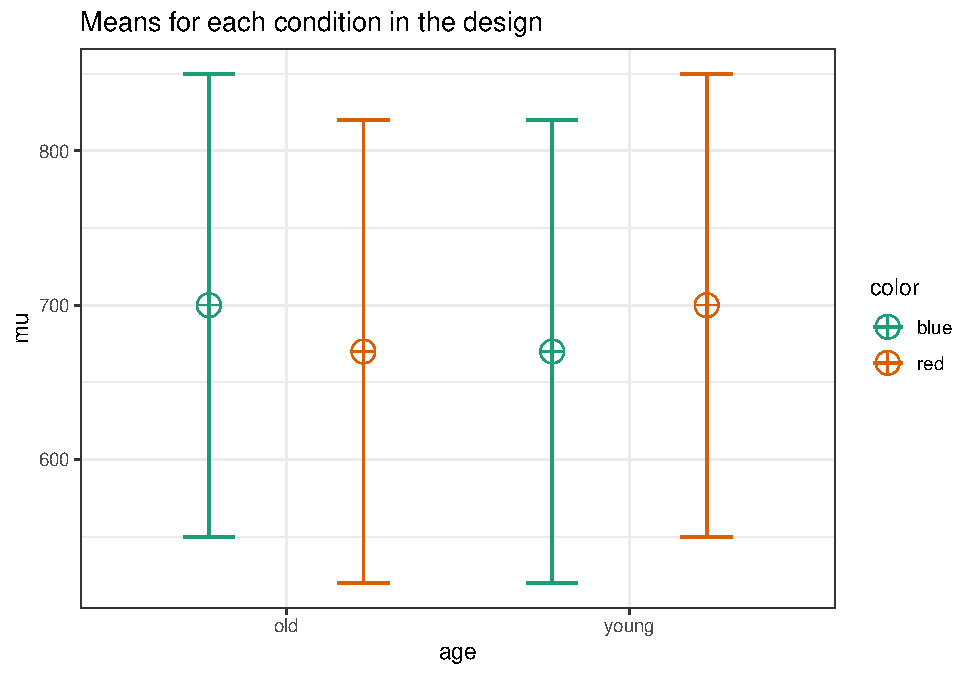
\includegraphics{SuperpowerValidation_files/figure-latex/unnamed-chunk-54-1.pdf}

\begin{Shaded}
\begin{Highlighting}[]
\NormalTok{simulation_result <-}\StringTok{ }\KeywordTok{ANOVA_power}\NormalTok{(design_result, }\DataTypeTok{alpha =} \FloatTok{0.05}\NormalTok{, }\DataTypeTok{nsims =}\NormalTok{ nsims)}
\end{Highlighting}
\end{Shaded}

\begin{verbatim}
## Power and Effect sizes for ANOVA tests
##                 power effect_size
## anova_age           5     0.03539
## anova_color         7     0.04235
## anova_age:color    43     0.16063
## 
## Power and Effect sizes for contrasts
##                                            power effect_size
## p_age_old_color_blue_age_old_color_red        19   -0.277372
## p_age_old_color_blue_age_young_color_blue     23   -0.275603
## p_age_old_color_blue_age_young_color_red       6    0.024031
## p_age_old_color_red_age_young_color_blue       4   -0.009016
## p_age_old_color_red_age_young_color_red       28    0.310872
## p_age_young_color_blue_age_young_color_red    28    0.309777
## 
## Within-Subject Factors Included: Check MANOVA Results
\end{verbatim}

The simulations yield closely matching results.

\hypertarget{examine-variation-of-means-and-correlation}{%
\section{Examine variation of means and correlation}\label{examine-variation-of-means-and-correlation}}

\begin{Shaded}
\begin{Highlighting}[]
\CommentTok{# define the parameters}
\NormalTok{mu =}\StringTok{ }\KeywordTok{c}\NormalTok{(}\DecValTok{700}\NormalTok{, }\DecValTok{670}\NormalTok{, }\DecValTok{690}\NormalTok{, }\DecValTok{750}\NormalTok{) }\CommentTok{# true effects (in this case, a double dissociation)}
\NormalTok{sigma =}\StringTok{ }\DecValTok{150}  \CommentTok{# population standard deviation}
\NormalTok{rho =}\StringTok{ }\FloatTok{0.4} \CommentTok{# correlation between repeated measures}
\NormalTok{nsubs =}\StringTok{ }\DecValTok{25} \CommentTok{# how many subjects?}
\NormalTok{nsims =}\StringTok{ }\NormalTok{nsims }\CommentTok{# how many simulation replicates?}
 
\CommentTok{# create 2 factors representing the 2 independent variables}
\NormalTok{cond =}\StringTok{ }\KeywordTok{data.frame}\NormalTok{(}
  \DataTypeTok{X1 =} \KeywordTok{rep}\NormalTok{(}\KeywordTok{factor}\NormalTok{(letters[}\DecValTok{1}\OperatorTok{:}\DecValTok{2}\NormalTok{]), nsubs }\OperatorTok{*}\StringTok{ }\DecValTok{2}\NormalTok{),}
  \DataTypeTok{X2 =} \KeywordTok{rep}\NormalTok{(}\KeywordTok{factor}\NormalTok{(letters[}\DecValTok{1}\OperatorTok{:}\DecValTok{2}\NormalTok{]), nsubs, }\DataTypeTok{each=}\DecValTok{2}\NormalTok{))}
 
\CommentTok{# create a subjects factor}
\NormalTok{subject =}\StringTok{ }\KeywordTok{factor}\NormalTok{(}\KeywordTok{sort}\NormalTok{(}\KeywordTok{rep}\NormalTok{(}\DecValTok{1}\OperatorTok{:}\NormalTok{nsubs, }\DecValTok{4}\NormalTok{)))}
 
\CommentTok{# combine above into the design matrix}
\NormalTok{dm =}\StringTok{ }\KeywordTok{data.frame}\NormalTok{(subject, cond)}
\end{Highlighting}
\end{Shaded}

Build Sigma: the population variance-covariance matrix

\begin{Shaded}
\begin{Highlighting}[]
\CommentTok{# create k x k matrix populated with sigma}
\NormalTok{sigma.mat <-}\StringTok{ }\KeywordTok{rep}\NormalTok{(sigma, }\DecValTok{4}\NormalTok{)}
\NormalTok{S <-}\StringTok{ }\KeywordTok{matrix}\NormalTok{(sigma.mat, }\DataTypeTok{ncol=}\KeywordTok{length}\NormalTok{(sigma.mat), }\DataTypeTok{nrow=}\KeywordTok{length}\NormalTok{(sigma.mat))}
 
\CommentTok{# compute covariance between measures}
\NormalTok{Sigma <-}\StringTok{ }\KeywordTok{t}\NormalTok{(S) }\OperatorTok{*}\StringTok{ }\NormalTok{S }\OperatorTok{*}\StringTok{ }\NormalTok{rho  }
 
\CommentTok{# put the variances on the diagonal }
\KeywordTok{diag}\NormalTok{(Sigma) <-}\StringTok{ }\NormalTok{sigma}\OperatorTok{^}\DecValTok{2}  
\end{Highlighting}
\end{Shaded}

Run the simulation

\begin{Shaded}
\begin{Highlighting}[]
\CommentTok{# stack 'nsims' individual data frames into one large data frame}
\NormalTok{df =}\StringTok{ }\NormalTok{dm[}\KeywordTok{rep}\NormalTok{(}\KeywordTok{seq_len}\NormalTok{(}\KeywordTok{nrow}\NormalTok{(dm)), nsims), ]}
 
\CommentTok{# add an index column to track the simulation run}
\NormalTok{df}\OperatorTok{$}\NormalTok{simID =}\StringTok{ }\KeywordTok{sort}\NormalTok{(}\KeywordTok{rep}\NormalTok{(}\KeywordTok{seq_len}\NormalTok{(nsims), }\KeywordTok{nrow}\NormalTok{(dm)))}
 
\CommentTok{# sample the observed data from a multivariate normal distribution}
\CommentTok{# using MASS::mvrnorm with the parameters mu and Sigma created earlier}
\CommentTok{# and bind to the existing df}
 
\KeywordTok{require}\NormalTok{(MASS)}
\NormalTok{make.y =}\StringTok{ }\KeywordTok{expression}\NormalTok{(}\KeywordTok{as.vector}\NormalTok{(}\KeywordTok{t}\NormalTok{(}\KeywordTok{mvrnorm}\NormalTok{(nsubs, mu, Sigma))))}
\NormalTok{df}\OperatorTok{$}\NormalTok{y =}\StringTok{ }\KeywordTok{as.vector}\NormalTok{(}\KeywordTok{replicate}\NormalTok{(nsims, }\KeywordTok{eval}\NormalTok{(make.y)))             }
 
\CommentTok{# use do(), the general purpose complement to the specialized data }
\CommentTok{# manipulation functions available in dplyr, to run the ANOVA on}
\CommentTok{# each section of the grouped data frame created by group_by}
 
\KeywordTok{require}\NormalTok{(dplyr)}
\KeywordTok{require}\NormalTok{(car)}
\KeywordTok{require}\NormalTok{(broom)}
 
\NormalTok{mods <-}\StringTok{ }\NormalTok{df }\OperatorTok\StringTok{ }
\StringTok{  }\KeywordTok{group_by}\NormalTok{(simID) }\OperatorTok\StringTok{ }
\StringTok{    }\KeywordTok{do}\NormalTok{(}\DataTypeTok{model =} \KeywordTok{aov}\NormalTok{(y }\OperatorTok{~}\StringTok{ }\NormalTok{X1 }\OperatorTok{*}\StringTok{ }\NormalTok{X2 }\OperatorTok{+}\StringTok{ }\KeywordTok{Error}\NormalTok{(subject }\OperatorTok{/}\StringTok{ }\NormalTok{(X1}\OperatorTok{*}\NormalTok{X2)), }\DataTypeTok{qr=}\OtherTok{FALSE}\NormalTok{, }\DataTypeTok{data =}\NormalTok{ .)) }
 
\CommentTok{# extract p-values for each effect and store in a data frame}
\NormalTok{p =}\StringTok{ }\KeywordTok{data.frame}\NormalTok{(}
\NormalTok{  mods }\OperatorTok\StringTok{ }\KeywordTok{do}\NormalTok{(}\KeywordTok{as.data.frame}\NormalTok{(}\KeywordTok{tidy}\NormalTok{(.}\OperatorTok{$}\NormalTok{model[[}\DecValTok{3}\NormalTok{]])}\OperatorTok{$}\NormalTok{p.value[}\DecValTok{1}\NormalTok{])),}
\NormalTok{  mods }\OperatorTok\StringTok{ }\KeywordTok{do}\NormalTok{(}\KeywordTok{as.data.frame}\NormalTok{(}\KeywordTok{tidy}\NormalTok{(.}\OperatorTok{$}\NormalTok{model[[}\DecValTok{4}\NormalTok{]])}\OperatorTok{$}\NormalTok{p.value[}\DecValTok{1}\NormalTok{])),}
\NormalTok{  mods }\OperatorTok\StringTok{ }\KeywordTok{do}\NormalTok{(}\KeywordTok{as.data.frame}\NormalTok{(}\KeywordTok{tidy}\NormalTok{(.}\OperatorTok{$}\NormalTok{model[[}\DecValTok{5}\NormalTok{]])}\OperatorTok{$}\NormalTok{p.value[}\DecValTok{1}\NormalTok{])))}
\KeywordTok{colnames}\NormalTok{(p) =}\StringTok{ }\KeywordTok{c}\NormalTok{(}\StringTok{'X1'}\NormalTok{,}\StringTok{'X2'}\NormalTok{,}\StringTok{'Interaction'}\NormalTok{)}
\end{Highlighting}
\end{Shaded}

The empirical power is easy to compute, it's just the proportion of simulation runs where p \textless. 05.

\begin{Shaded}
\begin{Highlighting}[]
\NormalTok{power.res =}\StringTok{ }\KeywordTok{apply}\NormalTok{(}\KeywordTok{as.matrix}\NormalTok{(p), }\DecValTok{2}\NormalTok{, }
  \ControlFlowTok{function}\NormalTok{(x) }\KeywordTok{round}\NormalTok{(}\KeywordTok{mean}\NormalTok{(}\KeywordTok{ifelse}\NormalTok{(x }\OperatorTok{<}\StringTok{ }\FloatTok{.05}\NormalTok{, }\DecValTok{1}\NormalTok{, }\DecValTok{0}\NormalTok{) }\OperatorTok{*}\StringTok{ }\DecValTok{100}\NormalTok{),}\DecValTok{2}\NormalTok{))}
\NormalTok{power.res}
\end{Highlighting}
\end{Shaded}

\begin{verbatim}
##          X1          X2 Interaction 
##           7          35          50
\end{verbatim}

Visualize the distributions of p-values

\begin{Shaded}
\begin{Highlighting}[]
\CommentTok{# plot the known effects}
\KeywordTok{require}\NormalTok{(ggplot2)}
\KeywordTok{require}\NormalTok{(gridExtra)}
 
\NormalTok{means =}\StringTok{ }\KeywordTok{data.frame}\NormalTok{(cond[}\DecValTok{1}\OperatorTok{:}\DecValTok{4}\NormalTok{, ], mu, }\DataTypeTok{SE =}\NormalTok{ sigma }\OperatorTok{/}\StringTok{ }\KeywordTok{sqrt}\NormalTok{(nsubs))}
\NormalTok{plt1 =}\StringTok{ }\KeywordTok{ggplot}\NormalTok{(means, }\KeywordTok{aes}\NormalTok{(}\DataTypeTok{y =}\NormalTok{ mu, }\DataTypeTok{x =}\NormalTok{ X1, }\DataTypeTok{fill=}\NormalTok{X2)) }\OperatorTok{+}
\StringTok{  }\KeywordTok{geom_bar}\NormalTok{(}\DataTypeTok{position =} \KeywordTok{position_dodge}\NormalTok{(), }\DataTypeTok{stat=}\StringTok{"identity"}\NormalTok{) }\OperatorTok{+}
\StringTok{  }\KeywordTok{geom_errorbar}\NormalTok{(}\KeywordTok{aes}\NormalTok{(}\DataTypeTok{ymin =}\NormalTok{ mu}\OperatorTok{-}\NormalTok{SE, }\DataTypeTok{ymax =}\NormalTok{ mu}\OperatorTok{+}\NormalTok{SE), }
    \DataTypeTok{position =} \KeywordTok{position_dodge}\NormalTok{(}\DataTypeTok{width=}\FloatTok{0.9}\NormalTok{), }\DataTypeTok{size=}\NormalTok{.}\DecValTok{6}\NormalTok{, }\DataTypeTok{width=}\NormalTok{.}\DecValTok{3}\NormalTok{) }\OperatorTok{+}
\StringTok{  }\KeywordTok{coord_cartesian}\NormalTok{(}\DataTypeTok{ylim=}\KeywordTok{c}\NormalTok{((.}\DecValTok{7}\OperatorTok{*}\KeywordTok{min}\NormalTok{(mu)), }\FloatTok{1.2}\OperatorTok{*}\KeywordTok{max}\NormalTok{(mu))) }\OperatorTok{+}
\StringTok{  }\KeywordTok{theme_bw}\NormalTok{()}
 
\CommentTok{# melt the data into a ggplot friendly 'long' format}
\KeywordTok{require}\NormalTok{(reshape2)}
\NormalTok{plotData <-}\StringTok{ }\KeywordTok{melt}\NormalTok{(p, }\DataTypeTok{value.name =} \StringTok{'p'}\NormalTok{)}
 
\CommentTok{# plot each of the p-value distributions on a log scale}
\KeywordTok{options}\NormalTok{(}\DataTypeTok{scipen =} \DecValTok{999}\NormalTok{) }\CommentTok{# 'turn off' scientific notation}
\NormalTok{plt2 =}\StringTok{ }\KeywordTok{ggplot}\NormalTok{(plotData, }\KeywordTok{aes}\NormalTok{(}\DataTypeTok{x =}\NormalTok{ p)) }\OperatorTok{+}
\StringTok{    }\KeywordTok{scale_x_log10}\NormalTok{(}\DataTypeTok{breaks=}\KeywordTok{c}\NormalTok{(}\DecValTok{1}\NormalTok{, }\FloatTok{0.05}\NormalTok{, }\FloatTok{0.001}\NormalTok{), }
                  \DataTypeTok{labels=}\KeywordTok{c}\NormalTok{(}\DecValTok{1}\NormalTok{, }\FloatTok{0.05}\NormalTok{, }\FloatTok{0.001}\NormalTok{)) }\OperatorTok{+}
\StringTok{    }\KeywordTok{geom_histogram}\NormalTok{(}\DataTypeTok{colour =} \StringTok{"darkblue"}\NormalTok{, }\DataTypeTok{fill =} \StringTok{"white"}\NormalTok{) }\OperatorTok{+}
\StringTok{    }\KeywordTok{geom_vline}\NormalTok{(}\DataTypeTok{xintercept =} \FloatTok{0.05}\NormalTok{, }\DataTypeTok{colour=}\StringTok{'red'}\NormalTok{) }\OperatorTok{+}
\StringTok{    }\KeywordTok{facet_grid}\NormalTok{(variable }\OperatorTok{~}\StringTok{ }\NormalTok{.) }\OperatorTok{+}
\StringTok{    }\KeywordTok{labs}\NormalTok{(}\DataTypeTok{x =} \KeywordTok{expression}\NormalTok{(Log[}\DecValTok{10}\NormalTok{]}\OperatorTok{~}\NormalTok{P)) }\OperatorTok{+}
\StringTok{    }\KeywordTok{theme}\NormalTok{(}\DataTypeTok{axis.text.x =} \KeywordTok{element_text}\NormalTok{(}\DataTypeTok{color=}\StringTok{'black'}\NormalTok{, }\DataTypeTok{size=}\DecValTok{7}\NormalTok{))}
 
\CommentTok{# arrange plots side by side and print}
\KeywordTok{grid.arrange}\NormalTok{(plt1, plt2, }\DataTypeTok{nrow=}\DecValTok{1}\NormalTok{)}
\end{Highlighting}
\end{Shaded}

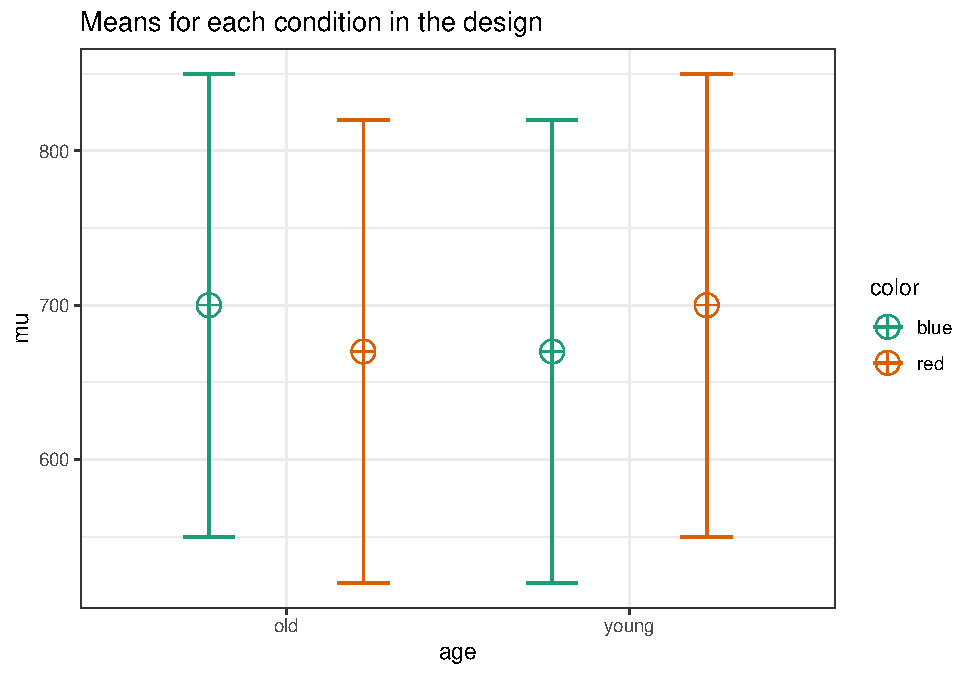
\includegraphics{SuperpowerValidation_files/figure-latex/unnamed-chunk-59-1.pdf}

We can reproduce this simulation:

\begin{Shaded}
\begin{Highlighting}[]
\NormalTok{mu =}\StringTok{ }\KeywordTok{c}\NormalTok{(}\DecValTok{700}\NormalTok{, }\DecValTok{670}\NormalTok{, }\DecValTok{690}\NormalTok{, }\DecValTok{750}\NormalTok{) }\CommentTok{# true effects (in this case, a double dissociation)}
\NormalTok{sigma =}\StringTok{ }\DecValTok{150}  \CommentTok{# population standard deviation}
\NormalTok{n <-}\StringTok{ }\DecValTok{25}
\NormalTok{sd <-}\StringTok{ }\DecValTok{150}
\NormalTok{r <-}\StringTok{ }\FloatTok{0.4}
\NormalTok{string =}\StringTok{ "2w*2w"}
\NormalTok{alpha_level <-}\StringTok{ }\FloatTok{0.05}
\NormalTok{labelnames =}\StringTok{ }\KeywordTok{c}\NormalTok{(}\StringTok{"age"}\NormalTok{, }\StringTok{"old"}\NormalTok{, }\StringTok{"young"}\NormalTok{, }\StringTok{"color"}\NormalTok{, }\StringTok{"blue"}\NormalTok{, }\StringTok{"red"}\NormalTok{)}
\NormalTok{design_result <-}\StringTok{ }\KeywordTok{ANOVA_design}\NormalTok{(}\DataTypeTok{design =}\NormalTok{ string,}
                              \DataTypeTok{n =}\NormalTok{ n, }
                              \DataTypeTok{mu =}\NormalTok{ mu, }
                              \DataTypeTok{sd =}\NormalTok{ sd, }
                              \DataTypeTok{r =}\NormalTok{ r, }
                              \DataTypeTok{labelnames =}\NormalTok{ labelnames)}
\end{Highlighting}
\end{Shaded}

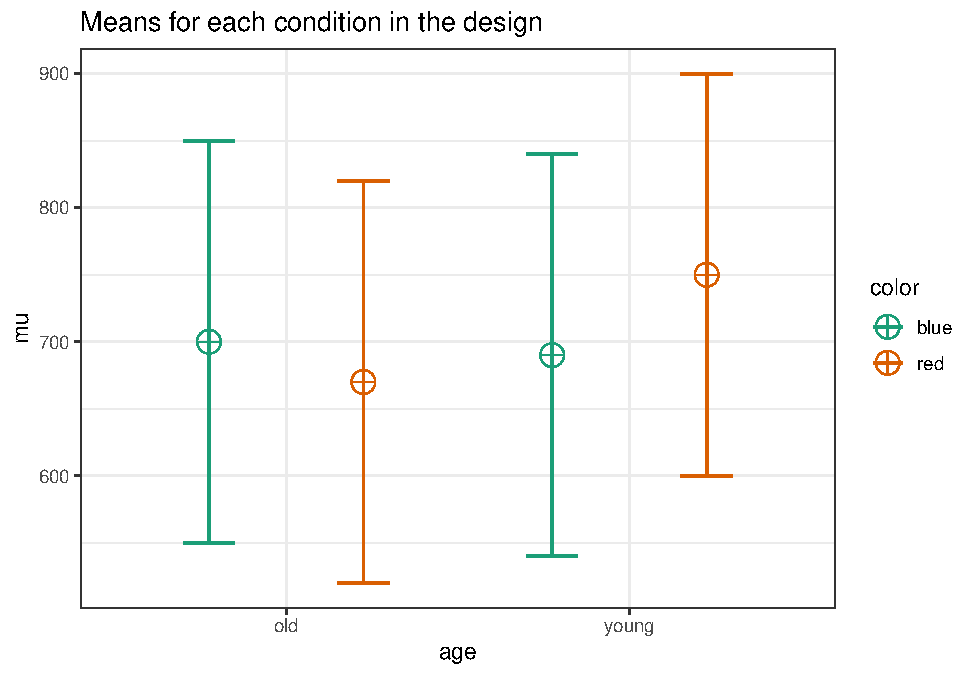
\includegraphics{SuperpowerValidation_files/figure-latex/unnamed-chunk-60-1.pdf}

\begin{Shaded}
\begin{Highlighting}[]
\NormalTok{simulation_result <-}\StringTok{ }\KeywordTok{ANOVA_power}\NormalTok{(design_result, }\DataTypeTok{alpha =} \FloatTok{0.05}\NormalTok{, }\DataTypeTok{nsims =}\NormalTok{ nsims)}
\end{Highlighting}
\end{Shaded}

\begin{verbatim}
## Power and Effect sizes for ANOVA tests
##                 power effect_size
## anova_age          29     0.10813
## anova_color        10     0.05224
## anova_age:color    43     0.14890
## 
## Power and Effect sizes for contrasts
##                                            power effect_size
## p_age_old_color_blue_age_old_color_red        16    -0.19631
## p_age_old_color_blue_age_young_color_blue      6    -0.05495
## p_age_old_color_blue_age_young_color_red      25     0.27436
## p_age_old_color_red_age_young_color_blue      11     0.13305
## p_age_old_color_red_age_young_color_red       57     0.46801
## p_age_young_color_blue_age_young_color_red    32     0.32829
## 
## Within-Subject Factors Included: Check MANOVA Results
\end{verbatim}

\hypertarget{mixed-anova-part-3}{%
\chapter{Mixed ANOVA Part 3}\label{mixed-anova-part-3}}

\hypertarget{two-by-two-anova-within-design}{%
\section{Two by two ANOVA, within design}\label{two-by-two-anova-within-design}}

Potvin \& Schutz (2000) simulate a wide range of repeated measure designs. The give an example of a 3x3 design, with the following correlation matrix:

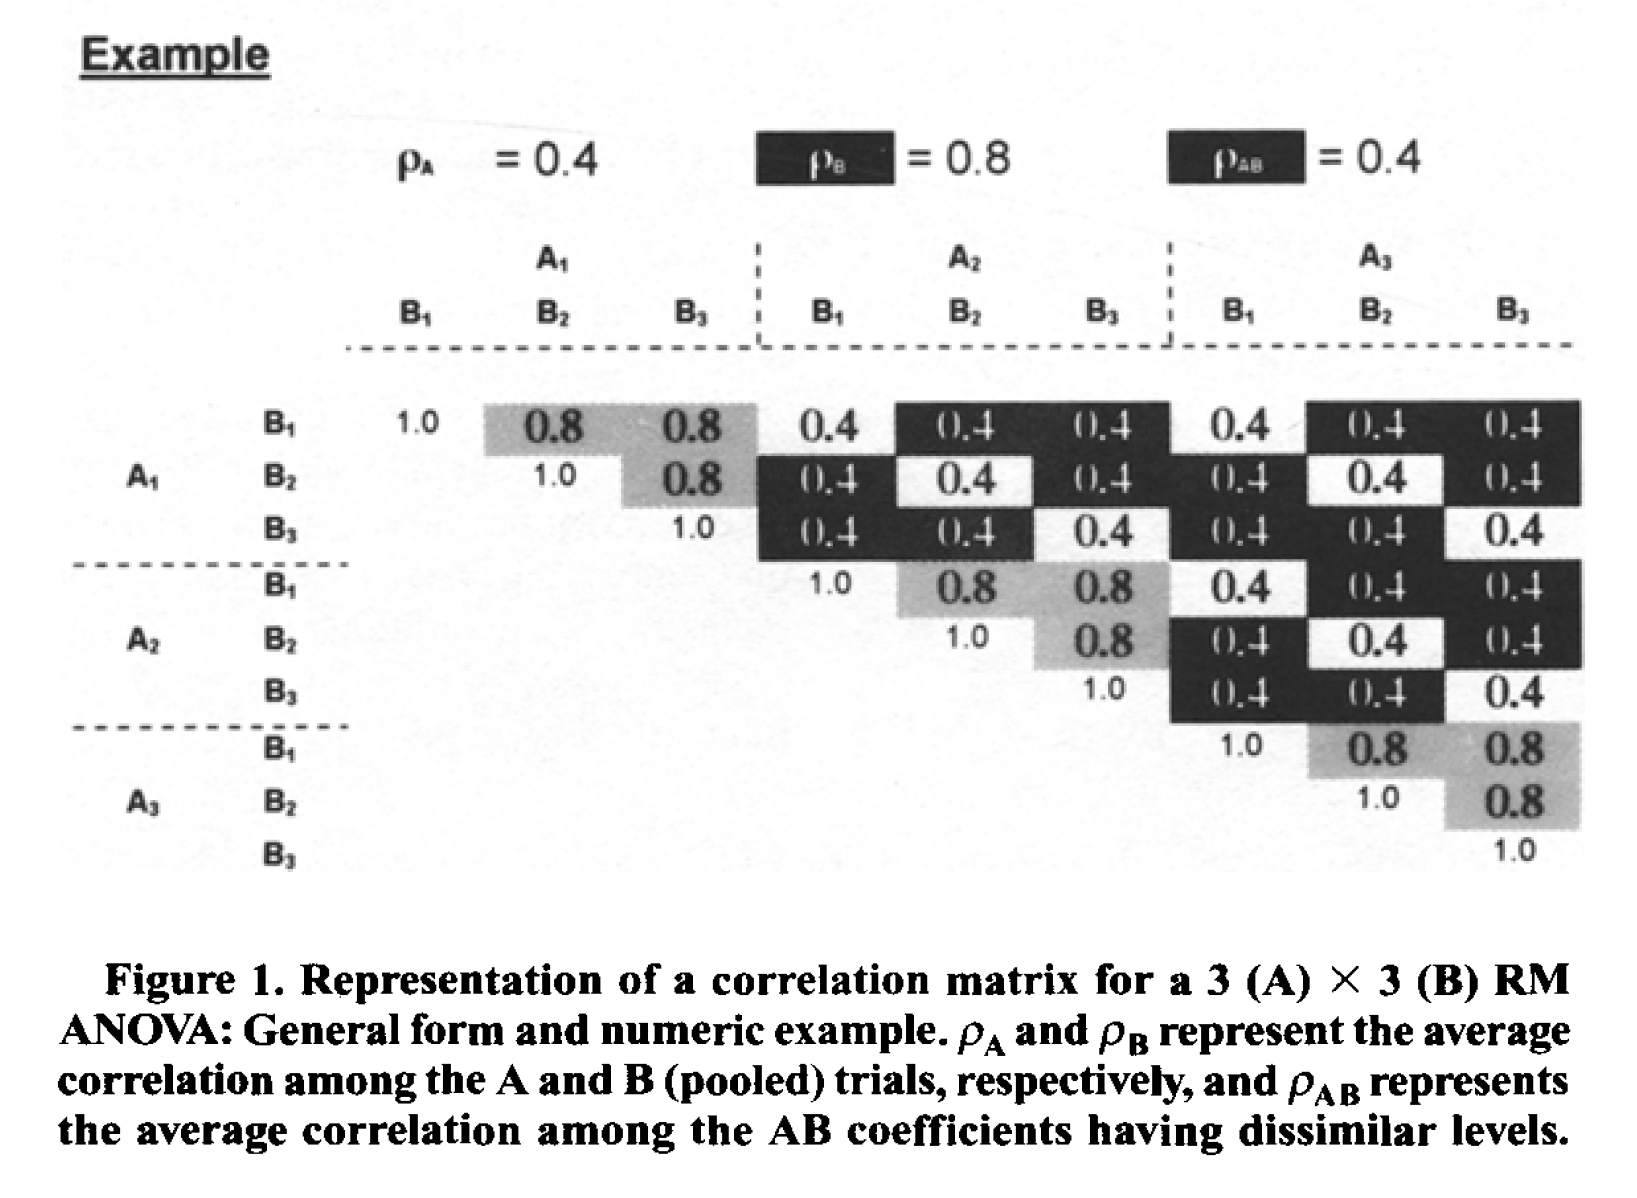
\includegraphics{screenshots/PS2000.png}

Variances were set to 1 (so all covariance matrices in their simulations were identical). In this specific example, the white fields are related to the correlation for the A main effect (these cells have the same level for B, but different levels of A). The grey cells are related to the main effect of B (the cells have the same level of A, but different levels of B). Finally, the black cells are related to the AxB interaction (they have different levels of A and B). The diagonal (all 1) relate to cells with the same levels of A and B.

Potvin \& Schulz (2000) examine power for 2x2 within ANOVA designs and develop approximations of the error variance. For a design with 2 within factors (A and B) these are:

For the main effect of A:
\(\sigma _ { e } ^ { 2 } = \sigma ^ { 2 } ( 1 - \overline { \rho } _ { A } ) + \sigma ^ { 2 } ( q - 1 ) ( \overline { \rho } _ { B } - \overline { \rho } _ { AB } )\)

For the main effectof B:
\(\sigma _ { e } ^ { 2 } = \sigma ^ { 2 } ( 1 - \overline { \rho } _ { B } ) + \sigma ^ { 2 } ( p - 1 ) ( \overline { \rho } _ { A } - \overline { \rho } _ { A B } )\)

For the interaction between A and B:
\(\sigma _ { e } ^ { 2 } = \sigma ^ { 2 } ( 1 - \rho _ { \max } ) - \sigma ^ { 2 } ( \overline { \rho } _ { \min } - \overline { \rho } _ { AB } )\)

\hypertarget{simple-example-2x2-within-design}{%
\chapter{Simple example: 2x2 within design}\label{simple-example-2x2-within-design}}

It is difficult to just come up with a positive definite covariance matrix. The best way to achieve this is to get the correlations from a pilot study. Indeed, it should be rather difficult to know which correlations to fill in without some pilot data.

We try to get the formulas in Potvin and Schutz (2000) working. \textbf{Below, I manage for the main effects, but not for the interaction}.

\begin{Shaded}
\begin{Highlighting}[]
\NormalTok{mu =}\StringTok{ }\KeywordTok{c}\NormalTok{(}\DecValTok{2}\NormalTok{,}\DecValTok{1}\NormalTok{,}\DecValTok{4}\NormalTok{,}\DecValTok{2}\NormalTok{) }
\NormalTok{n <-}\StringTok{ }\DecValTok{20}
\NormalTok{sd <-}\StringTok{ }\DecValTok{5}
\NormalTok{r <-}\StringTok{ }\KeywordTok{c}\NormalTok{(}
  \FloatTok{0.8}\NormalTok{, }\FloatTok{0.4}\NormalTok{, }\FloatTok{0.4}\NormalTok{,}
       \FloatTok{0.4}\NormalTok{, }\FloatTok{0.4}\NormalTok{,}
            \FloatTok{0.8}
\NormalTok{  )}
\NormalTok{string =}\StringTok{ "2w*2w"}
\NormalTok{alpha_level <-}\StringTok{ }\FloatTok{0.05}

\NormalTok{labelnames =}\StringTok{ }\KeywordTok{c}\NormalTok{(}\StringTok{"A"}\NormalTok{, }\StringTok{"a1"}\NormalTok{, }\StringTok{"a2"}\NormalTok{, }\StringTok{"B"}\NormalTok{, }\StringTok{"b1"}\NormalTok{, }\StringTok{"b2"}\NormalTok{)}
\NormalTok{design_result <-}\StringTok{ }\KeywordTok{ANOVA_design}\NormalTok{(}\DataTypeTok{design =}\NormalTok{ string,}
                              \DataTypeTok{n =}\NormalTok{ n, }
                              \DataTypeTok{mu =}\NormalTok{ mu, }
                              \DataTypeTok{sd =}\NormalTok{ sd, }
                              \DataTypeTok{r =}\NormalTok{ r, }
                              \DataTypeTok{labelnames =}\NormalTok{ labelnames)}
\end{Highlighting}
\end{Shaded}

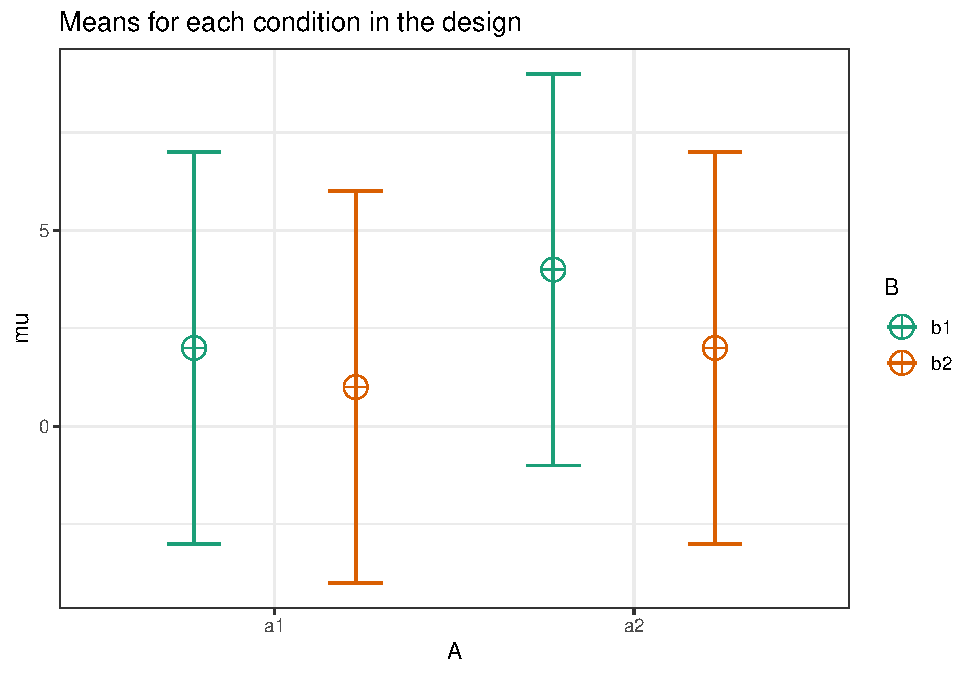
\includegraphics{SuperpowerValidation_files/figure-latex/unnamed-chunk-61-1.pdf}

\begin{Shaded}
\begin{Highlighting}[]
\NormalTok{simulation_result <-}\StringTok{ }\KeywordTok{ANOVA_power}\NormalTok{(design_result, }\DataTypeTok{alpha =} \FloatTok{0.05}\NormalTok{, }\DataTypeTok{nsims =} \DecValTok{1000}\NormalTok{)}
\end{Highlighting}
\end{Shaded}

\begin{verbatim}
## Power and Effect sizes for ANOVA tests
##           power effect_size
## anova_A    25.2     0.12701
## anova_B    80.9     0.33263
## anova_A:B  15.7     0.09032
## 
## Power and Effect sizes for contrasts
##                       power effect_size
## p_A_a1_B_b1_A_a1_B_b2  28.8   -0.337604
## p_A_a1_B_b1_A_a2_B_b1  34.6    0.384171
## p_A_a1_B_b1_A_a2_B_b2   6.1    0.003857
## p_A_a1_B_b2_A_a2_B_b1  65.2    0.577616
## p_A_a1_B_b2_A_a2_B_b2  13.2    0.197427
## p_A_a2_B_b1_A_a2_B_b2  75.9   -0.652759
## 
## Within-Subject Factors Included: Check MANOVA Results
\end{verbatim}

Result simulation after 100000 simulations

simulation\_result \textless- ANOVA\_power(design\_result, alpha = 0.05, nsims = 100000)
Power and Effect sizes for ANOVA tests
power effect size
anova\_A 26.849 0.0984
anova\_B 64.091 0.2452
anova\_A:B 26.875 0.0983

Power and Effect sizes for contrasts
power effect size
p\_A\_a1\_B\_b1\_A\_a1\_B\_b2 27.052 -0.3298
p\_A\_a1\_B\_b1\_A\_a2\_B\_b1 39.637 0.4162
p\_A\_a1\_B\_b1\_A\_a2\_B\_b2 4.983 -0.0005
p\_A\_a1\_B\_b2\_A\_a2\_B\_b1 64.252 0.5699
p\_A\_a1\_B\_b2\_A\_a2\_B\_b2 13.479 0.2077
p\_A\_a2\_B\_b1\_A\_a2\_B\_b2 76.622 -0.6597

We can try to use the formula in Potvin \& Schutz (2000).

\begin{Shaded}
\begin{Highlighting}[]
\NormalTok{k <-}\StringTok{ }\DecValTok{1} \CommentTok{#one group (because all factors are within)}
\NormalTok{rho_A <-}\StringTok{ }\FloatTok{0.5} \CommentTok{#mean r for factor A}
\NormalTok{rho_B <-}\StringTok{ }\FloatTok{0.8} \CommentTok{#mean r for factor B}
\NormalTok{rho_AB <-}\StringTok{ }\FloatTok{0.4} \CommentTok{#mean r for factor AB}
\NormalTok{alpha <-}\StringTok{ }\FloatTok{0.05}
\NormalTok{sigma <-}\StringTok{ }\NormalTok{sd}
\NormalTok{m_A <-}\StringTok{ }\DecValTok{2} \CommentTok{#levels factor A}
\NormalTok{variance_e_A <-}\StringTok{ }\NormalTok{sigma}\OperatorTok{^}\DecValTok{2} \OperatorTok{*}\StringTok{ }\NormalTok{(}\DecValTok{1} \OperatorTok{-}\StringTok{ }\NormalTok{rho_A) }\OperatorTok{+}\StringTok{ }\NormalTok{sigma}\OperatorTok{^}\DecValTok{2} \OperatorTok{*}\StringTok{ }\NormalTok{(m_A }\OperatorTok{-}\StringTok{ }\DecValTok{1}\NormalTok{) }\OperatorTok{*}\StringTok{ }\NormalTok{(rho_B }\OperatorTok{-}\StringTok{ }\NormalTok{rho_AB) }\CommentTok{#Variance A}
\NormalTok{variance_e_A}
\end{Highlighting}
\end{Shaded}

\begin{verbatim}
## [1] 22.5
\end{verbatim}

\begin{Shaded}
\begin{Highlighting}[]
\NormalTok{m_B <-}\StringTok{ }\DecValTok{2} \CommentTok{#levels factor B}
\NormalTok{variance_e_B <-}\StringTok{ }\NormalTok{sigma}\OperatorTok{^}\DecValTok{2} \OperatorTok{*}\StringTok{ }\NormalTok{(}\DecValTok{1} \OperatorTok{-}\StringTok{ }\NormalTok{rho_B) }\OperatorTok{+}\StringTok{ }\NormalTok{sigma}\OperatorTok{^}\DecValTok{2} \OperatorTok{*}\StringTok{ }\NormalTok{(m_B }\OperatorTok{-}\StringTok{ }\DecValTok{1}\NormalTok{) }\OperatorTok{*}\StringTok{ }\NormalTok{(rho_A }\OperatorTok{-}\StringTok{ }\NormalTok{rho_AB) }\CommentTok{#Variance B}
\NormalTok{variance_e_B}
\end{Highlighting}
\end{Shaded}

\begin{verbatim}
## [1] 7.5
\end{verbatim}

\begin{Shaded}
\begin{Highlighting}[]
\NormalTok{variance_e_AB <-}\StringTok{ }\NormalTok{sigma}\OperatorTok{^}\DecValTok{2} \OperatorTok{*}\StringTok{ }\NormalTok{(}\DecValTok{1} \OperatorTok{-}\StringTok{ }\KeywordTok{max}\NormalTok{(rho_A, rho_B)) }\OperatorTok{-}\StringTok{ }\NormalTok{sigma}\OperatorTok{^}\DecValTok{2} \OperatorTok{*}\StringTok{ }\NormalTok{(}\KeywordTok{min}\NormalTok{(rho_A, rho_B) }\OperatorTok{-}\StringTok{ }\NormalTok{rho_AB) }\CommentTok{#Variance AB}
\NormalTok{variance_e_AB}
\end{Highlighting}
\end{Shaded}

\begin{verbatim}
## [1] 2.5
\end{verbatim}

\begin{Shaded}
\begin{Highlighting}[]
\NormalTok{mean_mat <-}\StringTok{ }\KeywordTok{t}\NormalTok{(}\KeywordTok{matrix}\NormalTok{(mu, }\DataTypeTok{nrow =}\NormalTok{ m_B,}\DataTypeTok{ncol =}\NormalTok{ m_A)) }\CommentTok{#Create a mean matrix}
\NormalTok{mean_mat}
\end{Highlighting}
\end{Shaded}

\begin{verbatim}
##      [,1] [,2]
## [1,]    2    1
## [2,]    4    2
\end{verbatim}

\begin{Shaded}
\begin{Highlighting}[]
\CommentTok{# Potving & Schutz, 2000, formula 2, p. 348}
\CommentTok{# For main effect A}
\NormalTok{lambda_A <-}\StringTok{ }\NormalTok{n }\OperatorTok{*}\StringTok{ }\NormalTok{m_A }\OperatorTok{*}\StringTok{ }\KeywordTok{sum}\NormalTok{((}\KeywordTok{rowMeans}\NormalTok{(mean_mat) }\OperatorTok{-}\StringTok{ }\KeywordTok{mean}\NormalTok{(}\KeywordTok{rowMeans}\NormalTok{(mean_mat))) }\OperatorTok{^}\StringTok{ }\DecValTok{2}\NormalTok{) }\OperatorTok{/}\StringTok{ }\NormalTok{variance_e_A }
\NormalTok{lambda_A}
\end{Highlighting}
\end{Shaded}

\begin{verbatim}
## [1] 2
\end{verbatim}

\begin{Shaded}
\begin{Highlighting}[]
\NormalTok{df1 <-}\StringTok{ }\NormalTok{(m_A }\OperatorTok{-}\StringTok{ }\DecValTok{1}\NormalTok{) }\CommentTok{#calculate degrees of freedom 1 - ignoring the * e sphericity correction}
\NormalTok{df2 <-}\StringTok{ }\NormalTok{(n }\OperatorTok{-}\StringTok{ }\NormalTok{k) }\OperatorTok{*}\StringTok{ }\NormalTok{(m_A }\OperatorTok{-}\StringTok{ }\DecValTok{1}\NormalTok{) }\CommentTok{#calculate degrees of freedom 2}
\NormalTok{F_critical <-}\StringTok{ }\KeywordTok{qf}\NormalTok{(alpha, }\CommentTok{# critical F-vaue}
\NormalTok{                 df1,}
\NormalTok{                 df2, }
                 \DataTypeTok{lower.tail =} \OtherTok{FALSE}\NormalTok{) }
\NormalTok{pow_A <-}\StringTok{ }\KeywordTok{pf}\NormalTok{(}\KeywordTok{qf}\NormalTok{(alpha, }\CommentTok{#power }
\NormalTok{             df1, }
\NormalTok{             df2, }
             \DataTypeTok{lower.tail =} \OtherTok{FALSE}\NormalTok{), }
\NormalTok{          df1, }
\NormalTok{          df2, }
\NormalTok{          lambda_A, }
          \DataTypeTok{lower.tail =} \OtherTok{FALSE}\NormalTok{)}
\NormalTok{lambda_B <-}\StringTok{ }\NormalTok{n }\OperatorTok{*}\StringTok{ }\NormalTok{m_B }\OperatorTok{*}\StringTok{ }\KeywordTok{sum}\NormalTok{((}\KeywordTok{colMeans}\NormalTok{(mean_mat) }\OperatorTok{-}\StringTok{ }\KeywordTok{mean}\NormalTok{(}\KeywordTok{colMeans}\NormalTok{(mean_mat))) }\OperatorTok{^}\StringTok{ }\DecValTok{2}\NormalTok{) }\OperatorTok{/}\StringTok{ }\NormalTok{variance_e_B }
\NormalTok{lambda_B}
\end{Highlighting}
\end{Shaded}

\begin{verbatim}
## [1] 6
\end{verbatim}

\begin{Shaded}
\begin{Highlighting}[]
\NormalTok{df1 <-}\StringTok{ }\NormalTok{(m_B }\OperatorTok{-}\StringTok{ }\DecValTok{1}\NormalTok{) }\CommentTok{#calculate degrees of freedom 1}
\NormalTok{df2 <-}\StringTok{ }\NormalTok{(n }\OperatorTok{-}\StringTok{ }\NormalTok{k) }\OperatorTok{*}\StringTok{ }\NormalTok{(m_B }\OperatorTok{-}\StringTok{ }\DecValTok{1}\NormalTok{) }\CommentTok{#calculate degrees of freedom 2}
\NormalTok{F_critical <-}\StringTok{ }\KeywordTok{qf}\NormalTok{(alpha, }\CommentTok{# critical F-vaue}
\NormalTok{                 df1,}
\NormalTok{                 df2,}
                 \DataTypeTok{lower.tail =} \OtherTok{FALSE}\NormalTok{) }
\NormalTok{pow_B <-}\StringTok{ }\KeywordTok{pf}\NormalTok{(}\KeywordTok{qf}\NormalTok{(alpha, }\CommentTok{#power }
\NormalTok{             df1, }
\NormalTok{             df2, }
             \DataTypeTok{lower.tail =} \OtherTok{FALSE}\NormalTok{), }
\NormalTok{          df1, }
\NormalTok{          df2, }
\NormalTok{          lambda_B, }
          \DataTypeTok{lower.tail =} \OtherTok{FALSE}\NormalTok{)}
\NormalTok{pow_A}
\end{Highlighting}
\end{Shaded}

\begin{verbatim}
## [1] 0.2691752
\end{verbatim}

\begin{Shaded}
\begin{Highlighting}[]
\NormalTok{pow_B}
\end{Highlighting}
\end{Shaded}

\begin{verbatim}
## [1] 0.6422587
\end{verbatim}

We see the 26.9 and 64.2 correspond to the results of the simulation quite closely.

\begin{Shaded}
\begin{Highlighting}[]
\CommentTok{#This (or the variance calculation above) does not work. }
\NormalTok{lambda_AB <-}\StringTok{ }\NormalTok{n }\OperatorTok{*}\StringTok{ }\KeywordTok{sum}\NormalTok{((}
\NormalTok{  mean_mat }\OperatorTok{-}\StringTok{ }\KeywordTok{rowMeans}\NormalTok{(mean_mat) }\OperatorTok{-}\StringTok{ }\KeywordTok{colMeans}\NormalTok{(mean_mat) }\OperatorTok{+}\StringTok{ }\KeywordTok{mean}\NormalTok{(mean_mat)}
\NormalTok{  ) }\OperatorTok{^}\StringTok{ }\DecValTok{2}\NormalTok{) }\OperatorTok{/}\StringTok{ }\NormalTok{variance_e_AB }
\NormalTok{lambda_AB}
\end{Highlighting}
\end{Shaded}

\begin{verbatim}
## [1] 38
\end{verbatim}

\begin{Shaded}
\begin{Highlighting}[]
\NormalTok{df1 <-}\StringTok{ }\NormalTok{(m_A }\OperatorTok{-}\StringTok{ }\DecValTok{1}\NormalTok{)}\OperatorTok{*}\NormalTok{(m_B }\OperatorTok{-}\StringTok{ }\DecValTok{1}\NormalTok{)  }\CommentTok{#calculate degrees of freedom 1}
\NormalTok{df2 <-}\StringTok{ }\NormalTok{(n }\OperatorTok{-}\StringTok{ }\NormalTok{k) }\OperatorTok{*}\StringTok{ }\NormalTok{(m_A }\OperatorTok{-}\StringTok{ }\DecValTok{1}\NormalTok{) }\OperatorTok{*}\StringTok{ }\NormalTok{(m_B }\OperatorTok{-}\StringTok{ }\DecValTok{1}\NormalTok{) }\CommentTok{#calculate degrees of freedom 2}
\NormalTok{F_critical <-}\StringTok{ }\KeywordTok{qf}\NormalTok{(alpha, }\CommentTok{# critical F-vaue}
\NormalTok{                 df1,}
\NormalTok{                 df2, }
                 \DataTypeTok{lower.tail =} \OtherTok{FALSE}\NormalTok{) }
\NormalTok{pow <-}\StringTok{ }\KeywordTok{pf}\NormalTok{(}\KeywordTok{qf}\NormalTok{(alpha, }\CommentTok{#power }
\NormalTok{             df1, }
\NormalTok{             df2, }
             \DataTypeTok{lower.tail =} \OtherTok{FALSE}\NormalTok{), }
\NormalTok{          df1, }
\NormalTok{          df2, }
\NormalTok{          lambda_AB, }
          \DataTypeTok{lower.tail =} \OtherTok{FALSE}\NormalTok{)}
\NormalTok{pow}
\end{Highlighting}
\end{Shaded}

\begin{verbatim}
## [1] 0.9999458
\end{verbatim}

Maybe the simulation is not correct for the interaction, or the formula is not correctly programmed.

\hypertarget{error-control-in-exploratory-anova}{%
\chapter{Error Control in Exploratory ANOVA}\label{error-control-in-exploratory-anova}}

In a 2X2X2 design, an ANOVA will give the test results for three main effects, three two-way interactions, and one three-way interaction. That's 7 statistical tests. The probability of making at least one Type 1 error in a single 2x2x2 ANOVA is 1-(0.95)\^{}7 = 30\%.

\begin{Shaded}
\begin{Highlighting}[]
\NormalTok{string <-}\StringTok{ "2b*2b*2b"}
\NormalTok{n <-}\StringTok{ }\DecValTok{50}
\NormalTok{mu <-}\StringTok{ }\KeywordTok{c}\NormalTok{(}\DecValTok{20}\NormalTok{, }\DecValTok{20}\NormalTok{, }\DecValTok{20}\NormalTok{, }\DecValTok{20}\NormalTok{, }\DecValTok{20}\NormalTok{, }\DecValTok{20}\NormalTok{, }\DecValTok{20}\NormalTok{, }\DecValTok{20}\NormalTok{) }\CommentTok{#All means are equal - so there is no real difference.}
\CommentTok{# Enter means in the order that matches the labels below.}
\NormalTok{sd <-}\StringTok{ }\DecValTok{5}
\NormalTok{p_adjust =}\StringTok{ "none"}
\CommentTok{# "none" means we do not correct for multiple comparisons}
\NormalTok{labelnames <-}\StringTok{ }\KeywordTok{c}\NormalTok{(}\StringTok{"condition1"}\NormalTok{, }\StringTok{"a"}\NormalTok{, }\StringTok{"b"}\NormalTok{, }\StringTok{"condition2"}\NormalTok{, }\StringTok{"c"}\NormalTok{, }\StringTok{"d"}\NormalTok{, }\StringTok{"condition3"}\NormalTok{, }\StringTok{"e"}\NormalTok{, }\StringTok{"f"}\NormalTok{) }\CommentTok{#}
\CommentTok{# the label names should be in the order of the means specified above.}
\NormalTok{design_result <-}\StringTok{ }\KeywordTok{ANOVA_design}\NormalTok{(}\DataTypeTok{design =}\NormalTok{ string,}
                   \DataTypeTok{n =}\NormalTok{ n, }
                   \DataTypeTok{mu =}\NormalTok{ mu, }
                   \DataTypeTok{sd =}\NormalTok{ sd, }
                   \DataTypeTok{labelnames =}\NormalTok{ labelnames)}
\end{Highlighting}
\end{Shaded}

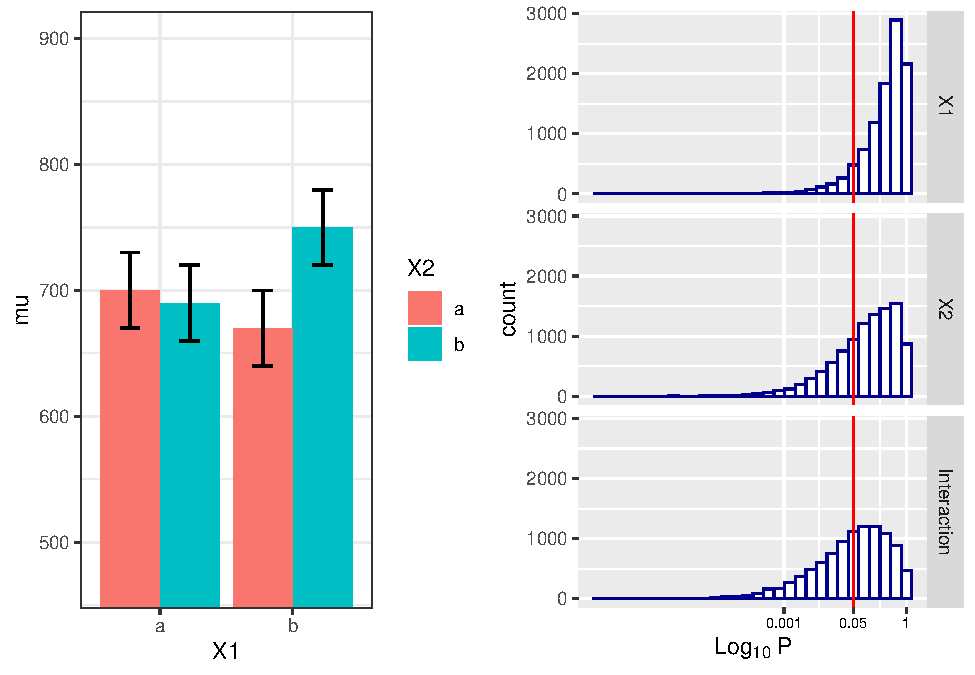
\includegraphics{SuperpowerValidation_files/figure-latex/unnamed-chunk-64-1.pdf}

\begin{Shaded}
\begin{Highlighting}[]
\NormalTok{alpha_level <-}\StringTok{ }\FloatTok{0.05}
\CommentTok{#We set the alpha level at 0.05. }
\NormalTok{power_result <-}\StringTok{ }\KeywordTok{ANOVA_power}\NormalTok{(design_result, }
                            \DataTypeTok{alpha_level =}\NormalTok{ alpha_level, }
                            \DataTypeTok{p_adjust =}\NormalTok{ p_adjust,}
                            \DataTypeTok{nsims =}\NormalTok{ nsims)}
\end{Highlighting}
\end{Shaded}

\begin{verbatim}
## Power and Effect sizes for ANOVA tests
##                                        power effect_size
## anova_condition1                           7    0.002448
## anova_condition2                           6    0.002890
## anova_condition3                           4    0.002388
## anova_condition1:condition2                5    0.002922
## anova_condition1:condition3                8    0.003331
## anova_condition2:condition3                5    0.002616
## anova_condition1:condition2:condition3     4    0.002362
## 
## Power and Effect sizes for contrasts
##                                                                                 power
## p_condition1_a_condition2_c_condition3_e_condition1_a_condition2_c_condition3_f     7
## p_condition1_a_condition2_c_condition3_e_condition1_a_condition2_d_condition3_e     5
## p_condition1_a_condition2_c_condition3_e_condition1_a_condition2_d_condition3_f     9
## p_condition1_a_condition2_c_condition3_e_condition1_b_condition2_c_condition3_e     9
## p_condition1_a_condition2_c_condition3_e_condition1_b_condition2_c_condition3_f     9
## p_condition1_a_condition2_c_condition3_e_condition1_b_condition2_d_condition3_e     6
## p_condition1_a_condition2_c_condition3_e_condition1_b_condition2_d_condition3_f     7
## p_condition1_a_condition2_c_condition3_f_condition1_a_condition2_d_condition3_e     4
## p_condition1_a_condition2_c_condition3_f_condition1_a_condition2_d_condition3_f     2
## p_condition1_a_condition2_c_condition3_f_condition1_b_condition2_c_condition3_e     5
## p_condition1_a_condition2_c_condition3_f_condition1_b_condition2_c_condition3_f     2
## p_condition1_a_condition2_c_condition3_f_condition1_b_condition2_d_condition3_e     3
## p_condition1_a_condition2_c_condition3_f_condition1_b_condition2_d_condition3_f     8
## p_condition1_a_condition2_d_condition3_e_condition1_a_condition2_d_condition3_f     3
## p_condition1_a_condition2_d_condition3_e_condition1_b_condition2_c_condition3_e     5
## p_condition1_a_condition2_d_condition3_e_condition1_b_condition2_c_condition3_f     3
## p_condition1_a_condition2_d_condition3_e_condition1_b_condition2_d_condition3_e     5
## p_condition1_a_condition2_d_condition3_e_condition1_b_condition2_d_condition3_f     5
## p_condition1_a_condition2_d_condition3_f_condition1_b_condition2_c_condition3_e     4
## p_condition1_a_condition2_d_condition3_f_condition1_b_condition2_c_condition3_f     5
## p_condition1_a_condition2_d_condition3_f_condition1_b_condition2_d_condition3_e     4
## p_condition1_a_condition2_d_condition3_f_condition1_b_condition2_d_condition3_f     3
## p_condition1_b_condition2_c_condition3_e_condition1_b_condition2_c_condition3_f     6
## p_condition1_b_condition2_c_condition3_e_condition1_b_condition2_d_condition3_e     5
## p_condition1_b_condition2_c_condition3_e_condition1_b_condition2_d_condition3_f     3
## p_condition1_b_condition2_c_condition3_f_condition1_b_condition2_d_condition3_e     5
## p_condition1_b_condition2_c_condition3_f_condition1_b_condition2_d_condition3_f     6
## p_condition1_b_condition2_d_condition3_e_condition1_b_condition2_d_condition3_f     6
##                                                                                 effect_size
## p_condition1_a_condition2_c_condition3_e_condition1_a_condition2_c_condition3_f   -0.033968
## p_condition1_a_condition2_c_condition3_e_condition1_a_condition2_d_condition3_e   -0.028220
## p_condition1_a_condition2_c_condition3_e_condition1_a_condition2_d_condition3_f   -0.029225
## p_condition1_a_condition2_c_condition3_e_condition1_b_condition2_c_condition3_e   -0.020848
## p_condition1_a_condition2_c_condition3_e_condition1_b_condition2_c_condition3_f   -0.005659
## p_condition1_a_condition2_c_condition3_e_condition1_b_condition2_d_condition3_e   -0.022539
## p_condition1_a_condition2_c_condition3_e_condition1_b_condition2_d_condition3_f   -0.021272
## p_condition1_a_condition2_c_condition3_f_condition1_a_condition2_d_condition3_e    0.002424
## p_condition1_a_condition2_c_condition3_f_condition1_a_condition2_d_condition3_f    0.001919
## p_condition1_a_condition2_c_condition3_f_condition1_b_condition2_c_condition3_e    0.010053
## p_condition1_a_condition2_c_condition3_f_condition1_b_condition2_c_condition3_f    0.024860
## p_condition1_a_condition2_c_condition3_f_condition1_b_condition2_d_condition3_e    0.010224
## p_condition1_a_condition2_c_condition3_f_condition1_b_condition2_d_condition3_f    0.010262
## p_condition1_a_condition2_d_condition3_e_condition1_a_condition2_d_condition3_f    0.001681
## p_condition1_a_condition2_d_condition3_e_condition1_b_condition2_c_condition3_e    0.008714
## p_condition1_a_condition2_d_condition3_e_condition1_b_condition2_c_condition3_f    0.021857
## p_condition1_a_condition2_d_condition3_e_condition1_b_condition2_d_condition3_e    0.007698
## p_condition1_a_condition2_d_condition3_e_condition1_b_condition2_d_condition3_f    0.008300
## p_condition1_a_condition2_d_condition3_f_condition1_b_condition2_c_condition3_e    0.009875
## p_condition1_a_condition2_d_condition3_f_condition1_b_condition2_c_condition3_f    0.022620
## p_condition1_a_condition2_d_condition3_f_condition1_b_condition2_d_condition3_e    0.003900
## p_condition1_a_condition2_d_condition3_f_condition1_b_condition2_d_condition3_f    0.005537
## p_condition1_b_condition2_c_condition3_e_condition1_b_condition2_c_condition3_f    0.012153
## p_condition1_b_condition2_c_condition3_e_condition1_b_condition2_d_condition3_e   -0.003082
## p_condition1_b_condition2_c_condition3_e_condition1_b_condition2_d_condition3_f   -0.003265
## p_condition1_b_condition2_c_condition3_f_condition1_b_condition2_d_condition3_e   -0.015912
## p_condition1_b_condition2_c_condition3_f_condition1_b_condition2_d_condition3_f   -0.014475
## p_condition1_b_condition2_d_condition3_e_condition1_b_condition2_d_condition3_f    0.000289
\end{verbatim}

When there is no true effect, we formally do not have `power' (which is defined as the probability of finding p \textless{} \(\alpha\) if there is a true effect to be found) so the power column should be read as the `Type 1 error rate'. Because we have saved the power simulation in the `power\_result' object, we can perform calculations on the `sim\_data' dataframe that is stored. This dataframe contains the results for the nsims simulations (e.g., 10000 rows if you ran 10000 simulations) and stores the p-values and effect size estimates for each ANOVA. The first 7 columns are the p-values for the ANOVA, first the main effects of condition 1, 2, and 3, then three two-way interactions, and finally the threeway interaction.

We can calculate the number of significant results for each test (which should be 5\%) by counting the number of significant p-values in each of the 7 rows:

\begin{Shaded}
\begin{Highlighting}[]
\KeywordTok{apply}\NormalTok{(}\KeywordTok{as.matrix}\NormalTok{(power_result}\OperatorTok{$}\NormalTok{sim_data[(}\DecValTok{1}\OperatorTok{:}\DecValTok{7}\NormalTok{)]), }\DecValTok{2}\NormalTok{, }
    \ControlFlowTok{function}\NormalTok{(x) }\KeywordTok{round}\NormalTok{(}\KeywordTok{mean}\NormalTok{(}\KeywordTok{ifelse}\NormalTok{(x }\OperatorTok{<}\StringTok{ }\NormalTok{alpha_level, }\DecValTok{1}\NormalTok{, }\DecValTok{0}\NormalTok{) }\OperatorTok{*}\StringTok{ }\DecValTok{100}\NormalTok{),}\DecValTok{4}\NormalTok{))}
\end{Highlighting}
\end{Shaded}

\begin{verbatim}
##                       anova_condition1 
##                                      7 
##                       anova_condition2 
##                                      6 
##                       anova_condition3 
##                                      4 
##            anova_condition1:condition2 
##                                      5 
##            anova_condition1:condition3 
##                                      8 
##            anova_condition2:condition3 
##                                      5 
## anova_condition1:condition2:condition3 
##                                      4
\end{verbatim}

This is the Type 1 error rate for each test. When we talk about error rate inflation due to multiple comparisons, we are talking about the probability that you conclude there is an effect, when there is actually no effect, when there is a significant effect for the main effect of condition 1, or condition 2, or condition 3, or for the two-way interaction between condition 1 and 2, or condition 1 and 3, or condition 2 and 3, or in the threeway interaction.

To calculate this error rate we do not just add the 7 error rates (so 7 * 5\% - 35\%). Instead, we calculate the probability that there will be at least one significant result in an ANOVA we perform. Some ANOVA results will have multiple significant results, just due to the Type 1 error rate (e.g., a significant result for the threeway interaction, and for the main effect of condition 1) but such an ANOVA is counted only once. Iwe calculate this percentage from our simulations, we see the number is indeed very close to 1-(0.95)\^{}7 = 30\%.

\begin{Shaded}
\begin{Highlighting}[]
\KeywordTok{sum}\NormalTok{(}\KeywordTok{apply}\NormalTok{(}\KeywordTok{as.matrix}\NormalTok{(power_result}\OperatorTok{$}\NormalTok{sim_data[(}\DecValTok{1}\OperatorTok{:}\DecValTok{7}\NormalTok{)]), }\DecValTok{1}\NormalTok{, }
    \ControlFlowTok{function}\NormalTok{(x) }\KeywordTok{round}\NormalTok{(}\KeywordTok{mean}\NormalTok{(}\KeywordTok{ifelse}\NormalTok{(x }\OperatorTok{<}\StringTok{ }\NormalTok{alpha_level, }\DecValTok{1}\NormalTok{, }\DecValTok{0}\NormalTok{) }\OperatorTok{*}\StringTok{ }\DecValTok{100}\NormalTok{),}\DecValTok{4}\NormalTok{)) }\OperatorTok{>}\StringTok{ }\DecValTok{0}\NormalTok{)}\OperatorTok{/}\NormalTok{nsims}\OperatorTok{*}\DecValTok{100}
\end{Highlighting}
\end{Shaded}

\begin{verbatim}
## [1] 33
\end{verbatim}

The question is what we should do about this alpha inflation. It is undesirable if you perform exploratory ANOVA's and are fooled too often by Type 1 errors, which will not replicate if you try to build on them. Therefore, you need to control the Type 1 error rate.

In the simulation code, which relies on the afex package, there is the option to set p\_adjust. In the simulation above, p\_adjust was set to ``none''. This means no adjustment is mage to which p-values are considered to be significant, and the alpha level is used as it is set in the simulation (above this was 0.05).

Afex relies on the p.adjust functon in the stats package in R (more information is available \href{https://www.rdocumentation.org/packages/stats/versions/3.1.1/topics/p.adjust}{here}). From the package details:

\emph{The adjustment methods include the Bonferroni correction (``bonferroni'') in which the p-values are multiplied by the number of comparisons. Less conservative corrections are also included by Holm (1979) (``holm''), Hochberg (1988) (``hochberg''), Hommel (1988) (``hommel''), Benjamini \& Hochberg (1995) (``BH'' or its alias ``fdr''), and Benjamini \& Yekutieli (2001) (``BY''), respectively. A pass-through option (``none'') is also included. The first four methods are designed to give strong control of the family-wise error rate. There seems no reason to use the unmodified Bonferroni correction because it is dominated by Holm's method, which is also valid under arbitrary assumptions.}

\emph{Hochberg's and Hommel's methods are valid when the hypothesis tests are independent or when they are non-negatively associated (Sarkar, 1998; Sarkar and Chang, 1997). Hommel's method is more powerful than Hochberg's, but the difference is usually small and the Hochberg p-values are faster to compute.}

\emph{The ``BH'' (aka ``fdr'') and ``BY'' method of Benjamini, Hochberg, and Yekutieli control the false discovery rate, the expected proportion of false discoveries amongst the rejected hypotheses. The false discovery rate is a less stringent condition than the family-wise error rate, so these methods are more powerful than the others.}

Let's re-run the simulation twith the Holm-Bonferroni correction, which is simple and require no assumptions.

\begin{Shaded}
\begin{Highlighting}[]
\NormalTok{string <-}\StringTok{ "2b*2b*2b"}
\NormalTok{n <-}\StringTok{ }\DecValTok{50}
\NormalTok{mu <-}\StringTok{ }\KeywordTok{c}\NormalTok{(}\DecValTok{20}\NormalTok{, }\DecValTok{20}\NormalTok{, }\DecValTok{20}\NormalTok{, }\DecValTok{20}\NormalTok{, }\DecValTok{20}\NormalTok{, }\DecValTok{20}\NormalTok{, }\DecValTok{20}\NormalTok{, }\DecValTok{20}\NormalTok{) }\CommentTok{#All means are equal - so there is no real difference.}
\CommentTok{# Enter means in the order that matches the labels below.}
\NormalTok{sd <-}\StringTok{ }\DecValTok{5}
\NormalTok{p_adjust =}\StringTok{ "holm"}
\CommentTok{# Changed to Holm-Bonferroni}
\NormalTok{labelnames <-}\StringTok{ }\KeywordTok{c}\NormalTok{(}\StringTok{"condition1"}\NormalTok{, }\StringTok{"a"}\NormalTok{, }\StringTok{"b"}\NormalTok{, }\StringTok{"condition2"}\NormalTok{, }\StringTok{"c"}\NormalTok{, }\StringTok{"d"}\NormalTok{, }\StringTok{"condition3"}\NormalTok{, }\StringTok{"e"}\NormalTok{, }\StringTok{"f"}\NormalTok{) }\CommentTok{#}
\CommentTok{# the label names should be in the order of the means specified above.}
\NormalTok{design_result <-}\StringTok{ }\KeywordTok{ANOVA_design}\NormalTok{(}\DataTypeTok{design =}\NormalTok{ string,}
                   \DataTypeTok{n =}\NormalTok{ n, }
                   \DataTypeTok{mu =}\NormalTok{ mu, }
                   \DataTypeTok{sd =}\NormalTok{ sd, }
                   \DataTypeTok{labelnames =}\NormalTok{ labelnames)}
\end{Highlighting}
\end{Shaded}

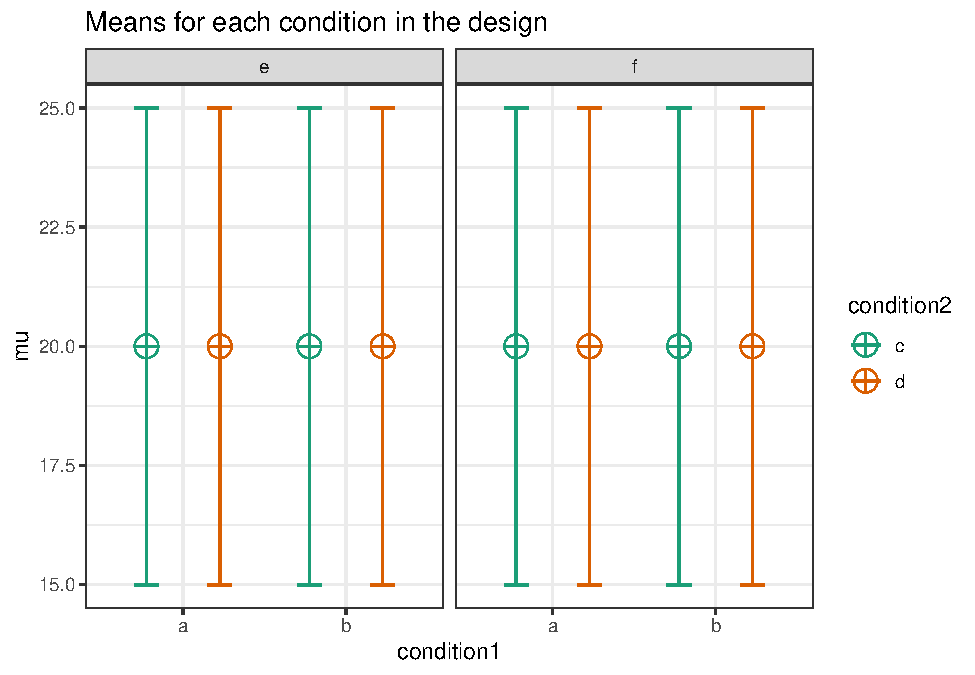
\includegraphics{SuperpowerValidation_files/figure-latex/unnamed-chunk-67-1.pdf}

\begin{Shaded}
\begin{Highlighting}[]
\NormalTok{alpha_level <-}\StringTok{ }\FloatTok{0.05}
\CommentTok{#We set the alpha level at 0.05. }
\NormalTok{power_result <-}\StringTok{ }\KeywordTok{ANOVA_power}\NormalTok{(design_result, }
                            \DataTypeTok{alpha_level =}\NormalTok{ alpha_level,}
                            \DataTypeTok{p_adjust =}\NormalTok{ p_adjust,}
                            \DataTypeTok{nsims =}\NormalTok{ nsims)}
\end{Highlighting}
\end{Shaded}

\begin{verbatim}
## Power and Effect sizes for ANOVA tests
##                                        power effect_size
## anova_condition1                           0    0.002118
## anova_condition2                           0    0.002285
## anova_condition3                           0    0.002092
## anova_condition1:condition2                1    0.002154
## anova_condition1:condition3                0    0.002392
## anova_condition2:condition3                1    0.002676
## anova_condition1:condition2:condition3     0    0.002047
## 
## Power and Effect sizes for contrasts
##                                                                                 power
## p_condition1_a_condition2_c_condition3_e_condition1_a_condition2_c_condition3_f     0
## p_condition1_a_condition2_c_condition3_e_condition1_a_condition2_d_condition3_e     0
## p_condition1_a_condition2_c_condition3_e_condition1_a_condition2_d_condition3_f     0
## p_condition1_a_condition2_c_condition3_e_condition1_b_condition2_c_condition3_e     0
## p_condition1_a_condition2_c_condition3_e_condition1_b_condition2_c_condition3_f     0
## p_condition1_a_condition2_c_condition3_e_condition1_b_condition2_d_condition3_e     0
## p_condition1_a_condition2_c_condition3_e_condition1_b_condition2_d_condition3_f     0
## p_condition1_a_condition2_c_condition3_f_condition1_a_condition2_d_condition3_e     0
## p_condition1_a_condition2_c_condition3_f_condition1_a_condition2_d_condition3_f     0
## p_condition1_a_condition2_c_condition3_f_condition1_b_condition2_c_condition3_e     0
## p_condition1_a_condition2_c_condition3_f_condition1_b_condition2_c_condition3_f     0
## p_condition1_a_condition2_c_condition3_f_condition1_b_condition2_d_condition3_e     0
## p_condition1_a_condition2_c_condition3_f_condition1_b_condition2_d_condition3_f     1
## p_condition1_a_condition2_d_condition3_e_condition1_a_condition2_d_condition3_f     0
## p_condition1_a_condition2_d_condition3_e_condition1_b_condition2_c_condition3_e     0
## p_condition1_a_condition2_d_condition3_e_condition1_b_condition2_c_condition3_f     0
## p_condition1_a_condition2_d_condition3_e_condition1_b_condition2_d_condition3_e     0
## p_condition1_a_condition2_d_condition3_e_condition1_b_condition2_d_condition3_f     0
## p_condition1_a_condition2_d_condition3_f_condition1_b_condition2_c_condition3_e     0
## p_condition1_a_condition2_d_condition3_f_condition1_b_condition2_c_condition3_f     0
## p_condition1_a_condition2_d_condition3_f_condition1_b_condition2_d_condition3_e     0
## p_condition1_a_condition2_d_condition3_f_condition1_b_condition2_d_condition3_f     0
## p_condition1_b_condition2_c_condition3_e_condition1_b_condition2_c_condition3_f     1
## p_condition1_b_condition2_c_condition3_e_condition1_b_condition2_d_condition3_e     0
## p_condition1_b_condition2_c_condition3_e_condition1_b_condition2_d_condition3_f     0
## p_condition1_b_condition2_c_condition3_f_condition1_b_condition2_d_condition3_e     0
## p_condition1_b_condition2_c_condition3_f_condition1_b_condition2_d_condition3_f     1
## p_condition1_b_condition2_d_condition3_e_condition1_b_condition2_d_condition3_f     0
##                                                                                 effect_size
## p_condition1_a_condition2_c_condition3_e_condition1_a_condition2_c_condition3_f   0.0154433
## p_condition1_a_condition2_c_condition3_e_condition1_a_condition2_d_condition3_e   0.0205541
## p_condition1_a_condition2_c_condition3_e_condition1_a_condition2_d_condition3_f   0.0422268
## p_condition1_a_condition2_c_condition3_e_condition1_b_condition2_c_condition3_e   0.0035021
## p_condition1_a_condition2_c_condition3_e_condition1_b_condition2_c_condition3_f   0.0044807
## p_condition1_a_condition2_c_condition3_e_condition1_b_condition2_d_condition3_e   0.0138438
## p_condition1_a_condition2_c_condition3_e_condition1_b_condition2_d_condition3_f  -0.0094933
## p_condition1_a_condition2_c_condition3_f_condition1_a_condition2_d_condition3_e   0.0053333
## p_condition1_a_condition2_c_condition3_f_condition1_a_condition2_d_condition3_f   0.0265343
## p_condition1_a_condition2_c_condition3_f_condition1_b_condition2_c_condition3_e  -0.0091160
## p_condition1_a_condition2_c_condition3_f_condition1_b_condition2_c_condition3_f  -0.0120365
## p_condition1_a_condition2_c_condition3_f_condition1_b_condition2_d_condition3_e  -0.0026837
## p_condition1_a_condition2_c_condition3_f_condition1_b_condition2_d_condition3_f  -0.0230180
## p_condition1_a_condition2_d_condition3_e_condition1_a_condition2_d_condition3_f   0.0204428
## p_condition1_a_condition2_d_condition3_e_condition1_b_condition2_c_condition3_e  -0.0169158
## p_condition1_a_condition2_d_condition3_e_condition1_b_condition2_c_condition3_f  -0.0190223
## p_condition1_a_condition2_d_condition3_e_condition1_b_condition2_d_condition3_e  -0.0070959
## p_condition1_a_condition2_d_condition3_e_condition1_b_condition2_d_condition3_f  -0.0292813
## p_condition1_a_condition2_d_condition3_f_condition1_b_condition2_c_condition3_e  -0.0365485
## p_condition1_a_condition2_d_condition3_f_condition1_b_condition2_c_condition3_f  -0.0382325
## p_condition1_a_condition2_d_condition3_f_condition1_b_condition2_d_condition3_e  -0.0288324
## p_condition1_a_condition2_d_condition3_f_condition1_b_condition2_d_condition3_f  -0.0504461
## p_condition1_b_condition2_c_condition3_e_condition1_b_condition2_c_condition3_f   0.0007649
## p_condition1_b_condition2_c_condition3_e_condition1_b_condition2_d_condition3_e   0.0091853
## p_condition1_b_condition2_c_condition3_e_condition1_b_condition2_d_condition3_f  -0.0144361
## p_condition1_b_condition2_c_condition3_f_condition1_b_condition2_d_condition3_e   0.0104412
## p_condition1_b_condition2_c_condition3_f_condition1_b_condition2_d_condition3_f  -0.0120434
## p_condition1_b_condition2_d_condition3_e_condition1_b_condition2_d_condition3_f  -0.0225975
\end{verbatim}

If we now calculate the overall Type 1 error rate:

\begin{Shaded}
\begin{Highlighting}[]
\KeywordTok{sum}\NormalTok{(}\KeywordTok{apply}\NormalTok{(}\KeywordTok{as.matrix}\NormalTok{(power_result}\OperatorTok{$}\NormalTok{sim_data[(}\DecValTok{1}\OperatorTok{:}\DecValTok{7}\NormalTok{)]), }\DecValTok{1}\NormalTok{, }
    \ControlFlowTok{function}\NormalTok{(x) }\KeywordTok{round}\NormalTok{(}\KeywordTok{mean}\NormalTok{(}\KeywordTok{ifelse}\NormalTok{(x }\OperatorTok{<}\StringTok{ }\NormalTok{alpha_level, }\DecValTok{1}\NormalTok{, }\DecValTok{0}\NormalTok{) }\OperatorTok{*}\StringTok{ }\DecValTok{100}\NormalTok{),}\DecValTok{4}\NormalTok{)) }\OperatorTok{>}\StringTok{ }\DecValTok{0}\NormalTok{)}\OperatorTok{/}\NormalTok{nsims}\OperatorTok{*}\DecValTok{100}
\end{Highlighting}
\end{Shaded}

\begin{verbatim}
## [1] 2
\end{verbatim}

We see it is close to 5\%. Note that error rates have variation, and even in a few thousand simulations, the error rate in the sample of studies can easily be half a percentage point higher or lower. But \emph{in the long run} the error rate should equal the alpha level. Furthermore, note that the \href{https://en.wikipedia.org/wiki/Holm\%E2\%80\%93Bonferroni_method}{Holm-bonferroni} method is slightly more powerful than the Bonferroni procedure (which is simply \(\alpha\) divided by the numner of tests). There are more powerful procedures to control the Type 1 error rate, which require more assumptions. For a small number of tests, they Holm-Bonferroni procedure works well. Alternative procedure to control error rates can be found in the \href{https://cran.r-project.org/web/packages/multcomp/index.html}{multcomp} R package.

\hypertarget{power-in-interactions}{%
\chapter{Power in Interactions}\label{power-in-interactions}}

In the 17th Data Colada blog post titled \href{http://datacolada.org/17}{No-way Interactions} Uri Simonsohn discusses how a moderated interaction (the effect is there in one condition, but disappears in another condition) requires at least twice as many subjects per cell as a study that simply aims to show the simple effect. For example, see the plot below. Assume the score on the vertical axis is desire for fruit, as a function of the fruit that is available (an apple or a banana) and how hungry people are (not, or very). We see there is a difference between the participants desire for a banana compared to an apple, but only for participants who are very hungry. The point that is made is that you need twice as many participants in each cell to have power for the interaction, as you need for the simple effect.

\begin{Shaded}
\begin{Highlighting}[]
\NormalTok{string <-}\StringTok{ "2b*2b"}
\NormalTok{n <-}\StringTok{ }\DecValTok{20}
\NormalTok{mu <-}\StringTok{ }\KeywordTok{c}\NormalTok{(}\DecValTok{20}\NormalTok{, }\DecValTok{20}\NormalTok{, }\DecValTok{20}\NormalTok{, }\DecValTok{25}\NormalTok{) }\CommentTok{#All means are equal - so there is no real difference.}
\CommentTok{# Enter means in the order that matches the labels below.}
\NormalTok{sd <-}\StringTok{ }\FloatTok{0.5}
\NormalTok{labelnames <-}\StringTok{ }\KeywordTok{c}\NormalTok{(}\StringTok{"fruit"}\NormalTok{, }\StringTok{"apple"}\NormalTok{, }\StringTok{"banana"}\NormalTok{, }\StringTok{"hunger"}\NormalTok{, }\StringTok{"no hunger"}\NormalTok{, }\StringTok{"very hungry"}\NormalTok{) }\CommentTok{#}
\CommentTok{# the label names should be in the order of the means specified above.}
\NormalTok{design_result <-}\StringTok{ }\KeywordTok{ANOVA_design}\NormalTok{(}\DataTypeTok{design =}\NormalTok{ string,}
                   \DataTypeTok{n =}\NormalTok{ n, }
                   \DataTypeTok{mu =}\NormalTok{ mu, }
                   \DataTypeTok{sd =}\NormalTok{ sd, }
                   \DataTypeTok{labelnames =}\NormalTok{ labelnames)}
\end{Highlighting}
\end{Shaded}

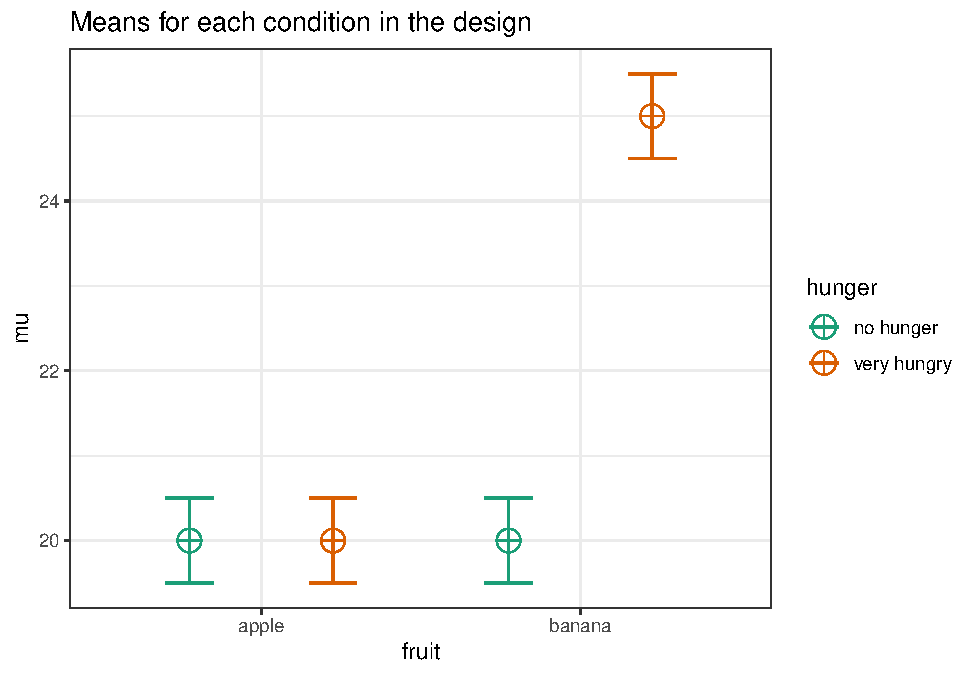
\includegraphics{SuperpowerValidation_files/figure-latex/unnamed-chunk-69-1.pdf}

We can reproduce the simulations in the Data Colada blog post, using the original code.

\begin{Shaded}
\begin{Highlighting}[]
\CommentTok{#R-Code}
\CommentTok{#}
\CommentTok{#Written by Uri Simonsohn, March 2014}
\CommentTok{#}
\CommentTok{#}
\CommentTok{#In DataColada[17] I propose that 2x2 interaction studies need 2x the sample size}
\CommentTok{#http://datacolada.org/2014/03/10/17-no-way-interactions}
\CommentTok{#In a companion ,pdf I show the simple math behind it}
\CommentTok{#}
\CommentTok{#}
\CommentTok{#Simulations are often more persuasive than math, so here it goes.}
\CommentTok{#I run simulations that compute power for 2 and 4 cell design, the latter testing the interaction}
\CommentTok{###################################################################################################}
\CommentTok{#Create function that computes power of Studies 1 and 2, where Study 1  has 2 cells and tests a simple effect}
\CommentTok{#and Study 2 has 4 cells and tests the interaction}
\NormalTok{  colada17=}\ControlFlowTok{function}\NormalTok{(d1,d2,n1,n2,simtot)}
\NormalTok{  \{}
  \CommentTok{#n1: sample size, per cell, study 1}
  \CommentTok{#n2: sample size, per cell, study 2}
  \CommentTok{#d1: simple effect M1-M2}
  \CommentTok{#d2: moderated effect M3-M4, full elimination of effect implies d2=0}
  \CommentTok{#simtot: how many simulations to run}
  \CommentTok{#Here we will store results}
\NormalTok{      p1=}\KeywordTok{c}\NormalTok{()    }\CommentTok{#p-values for Study 1}
\NormalTok{      p2=}\KeywordTok{c}\NormalTok{()    }\CommentTok{#p-values for Study 2}
  \ControlFlowTok{for}\NormalTok{(i }\ControlFlowTok{in} \DecValTok{1}\OperatorTok{:}\NormalTok{simtot) \{}
    \CommentTok{#draw data 4 samples}
\NormalTok{    y1=}\KeywordTok{rnorm}\NormalTok{(}\DataTypeTok{n=}\KeywordTok{max}\NormalTok{(n1,n2),}\DataTypeTok{mean=}\NormalTok{d1)}
\NormalTok{    y2=}\KeywordTok{rnorm}\NormalTok{(}\DataTypeTok{n=}\KeywordTok{max}\NormalTok{(n1,n2))}
\NormalTok{    y3=}\KeywordTok{rnorm}\NormalTok{(}\DataTypeTok{n=}\KeywordTok{max}\NormalTok{(n1,n2),}\DataTypeTok{mean=}\NormalTok{d2)}
\NormalTok{    y4=}\KeywordTok{rnorm}\NormalTok{(}\DataTypeTok{n=}\KeywordTok{max}\NormalTok{(n1,n2))}
    
    \CommentTok{#GET DATA READY FOR ANOVA  }
\NormalTok{      y=}\KeywordTok{c}\NormalTok{(y1,y2,y3,y4)          }\CommentTok{#the d.v.}
\NormalTok{      nrep=}\KeywordTok{rep}\NormalTok{(n2,}\DecValTok{4}\NormalTok{)          }
\NormalTok{      A=}\KeywordTok{rep}\NormalTok{(}\KeywordTok{c}\NormalTok{(}\DecValTok{1}\NormalTok{,}\DecValTok{1}\NormalTok{,}\DecValTok{0}\NormalTok{,}\DecValTok{0}\NormalTok{),}\DataTypeTok{times=}\NormalTok{nrep) }
\NormalTok{      B=}\KeywordTok{rep}\NormalTok{(}\KeywordTok{c}\NormalTok{(}\DecValTok{1}\NormalTok{,}\DecValTok{0}\NormalTok{,}\DecValTok{1}\NormalTok{,}\DecValTok{0}\NormalTok{),}\DataTypeTok{times=}\NormalTok{nrep)}
    
    \CommentTok{#STUDY 1}
\NormalTok{      p1.k=}\KeywordTok{t.test}\NormalTok{(y1[}\DecValTok{1}\OperatorTok{:}\NormalTok{n1],y2[}\DecValTok{1}\OperatorTok{:}\NormalTok{n1],}\DataTypeTok{var.equal=}\OtherTok{TRUE}\NormalTok{)}\OperatorTok{$}\NormalTok{p.value  }\CommentTok{#Do a t-test on the first n1 observations}
    
    \CommentTok{#STUDY 2}
\NormalTok{      p2.k=}\KeywordTok{anova}\NormalTok{(}\KeywordTok{lm}\NormalTok{(y }\OperatorTok{~}\StringTok{ }\NormalTok{A }\OperatorTok{*}\StringTok{ }\NormalTok{B))[}\StringTok{"A:B"}\NormalTok{, }\StringTok{"Pr(>F)"}\NormalTok{]             }\CommentTok{#Do anova, keep p-value of the interaction}
        
      \CommentTok{#Store the results}
\NormalTok{      p1=}\KeywordTok{c}\NormalTok{(p1,p1.k)}
\NormalTok{      p2=}\KeywordTok{c}\NormalTok{(p2,p2.k)}
    
\NormalTok{      \}}
  
  \CommentTok{#What share off comparisons are significant}
\NormalTok{    power1=}\KeywordTok{sum}\NormalTok{(p1}\OperatorTok{<=}\NormalTok{.}\DecValTok{05}\NormalTok{)}\OperatorTok{/}\NormalTok{simtot  }\CommentTok{#Simple test using estimate of variance from 2 cells only}
\NormalTok{    power2=}\KeywordTok{sum}\NormalTok{(p2}\OperatorTok{<=}\NormalTok{.}\DecValTok{05}\NormalTok{)}\OperatorTok{/}\NormalTok{simtot  }\CommentTok{#Interaction}
  
    \KeywordTok{cat}\NormalTok{(}\StringTok{"}\CharTok{\textbackslash{}n}\StringTok{Study 1 is powered to:"}\NormalTok{,}\KeywordTok{round}\NormalTok{(power1,}\DecValTok{2}\NormalTok{))}
    \KeywordTok{cat}\NormalTok{(}\StringTok{"}\CharTok{\textbackslash{}n}\StringTok{Study 2 is powered to:"}\NormalTok{,}\KeywordTok{round}\NormalTok{(power2,}\DecValTok{2}\NormalTok{))}
  
\NormalTok{    \}}
    
    
\CommentTok{#Same power for 2n regardless of n and d}
  \KeywordTok{colada17}\NormalTok{(}\DataTypeTok{simtot=}\DecValTok{2000}\NormalTok{, }\DataTypeTok{n1=}\DecValTok{20}\NormalTok{,}\DataTypeTok{n2=}\DecValTok{40}\NormalTok{,}\DataTypeTok{d1=}\DecValTok{1}\NormalTok{,}\DataTypeTok{d2=}\DecValTok{0}\NormalTok{)  }
\end{Highlighting}
\end{Shaded}

\begin{verbatim}
## 
## Study 1 is powered to: 0.87
## Study 2 is powered to: 0.9
\end{verbatim}

\begin{Shaded}
\begin{Highlighting}[]
  \KeywordTok{colada17}\NormalTok{(}\DataTypeTok{simtot=}\DecValTok{2000}\NormalTok{, }\DataTypeTok{n1=}\DecValTok{50}\NormalTok{,}\DataTypeTok{n2=}\DecValTok{100}\NormalTok{,}\DataTypeTok{d1=}\NormalTok{.}\DecValTok{3}\NormalTok{,}\DataTypeTok{d2=}\DecValTok{0}\NormalTok{)}
\end{Highlighting}
\end{Shaded}

\begin{verbatim}
## 
## Study 1 is powered to: 0.33
## Study 2 is powered to: 0.3
\end{verbatim}

\begin{Shaded}
\begin{Highlighting}[]
  \KeywordTok{colada17}\NormalTok{(}\DataTypeTok{simtot=}\DecValTok{2000}\NormalTok{, }\DataTypeTok{n1=}\DecValTok{150}\NormalTok{,}\DataTypeTok{n2=}\DecValTok{300}\NormalTok{,}\DataTypeTok{d1=}\NormalTok{.}\DecValTok{25}\NormalTok{,}\DataTypeTok{d2=}\DecValTok{0}\NormalTok{)}
\end{Highlighting}
\end{Shaded}

\begin{verbatim}
## 
## Study 1 is powered to: 0.58
## Study 2 is powered to: 0.59
\end{verbatim}

\begin{Shaded}
\begin{Highlighting}[]
\CommentTok{#Need 4n if effect is 70% attenuated}
  \KeywordTok{colada17}\NormalTok{(}\DataTypeTok{simtot=}\DecValTok{2000}\NormalTok{, }\DataTypeTok{n1=}\DecValTok{25}\NormalTok{,}\DataTypeTok{n2=}\DecValTok{100}\NormalTok{,}\DataTypeTok{d1=}\NormalTok{.}\DecValTok{5}\NormalTok{, }\DataTypeTok{d2=}\NormalTok{.}\DecValTok{3}\OperatorTok{*}\NormalTok{.}\DecValTok{5}\NormalTok{)}
\end{Highlighting}
\end{Shaded}

\begin{verbatim}
## 
## Study 1 is powered to: 0.39
## Study 2 is powered to: 0.41
\end{verbatim}

\begin{Shaded}
\begin{Highlighting}[]
  \KeywordTok{colada17}\NormalTok{(}\DataTypeTok{simtot=}\DecValTok{2000}\NormalTok{, }\DataTypeTok{n1=}\DecValTok{50}\NormalTok{,}\DataTypeTok{n2=}\DecValTok{200}\NormalTok{,}\DataTypeTok{d1=}\NormalTok{.}\DecValTok{5}\NormalTok{, }\DataTypeTok{d2=}\NormalTok{.}\DecValTok{3}\OperatorTok{*}\NormalTok{.}\DecValTok{5}\NormalTok{)}
\end{Highlighting}
\end{Shaded}

\begin{verbatim}
## 
## Study 1 is powered to: 0.7
## Study 2 is powered to: 0.68
\end{verbatim}

\begin{Shaded}
\begin{Highlighting}[]
  \KeywordTok{colada17}\NormalTok{(}\DataTypeTok{simtot=}\DecValTok{2000}\NormalTok{, }\DataTypeTok{n1=}\DecValTok{22}\NormalTok{,}\DataTypeTok{n2=}\DecValTok{88}\NormalTok{,}\DataTypeTok{d1=}\NormalTok{.}\DecValTok{41}\NormalTok{, }\DataTypeTok{d2=}\NormalTok{.}\DecValTok{3}\OperatorTok{*}\NormalTok{.}\DecValTok{41}\NormalTok{)}
\end{Highlighting}
\end{Shaded}

\begin{verbatim}
## 
## Study 1 is powered to: 0.26
## Study 2 is powered to: 0.27
\end{verbatim}

\begin{Shaded}
\begin{Highlighting}[]
\CommentTok{#underpowered if run with the same n}
\KeywordTok{colada17}\NormalTok{(}\DataTypeTok{simtot=}\NormalTok{nsims, }\DataTypeTok{n1=}\DecValTok{20}\NormalTok{,}\DataTypeTok{n2=}\DecValTok{20}\NormalTok{,}\DataTypeTok{d1=}\DecValTok{1}\NormalTok{,}\DataTypeTok{d2=}\DecValTok{0}\NormalTok{)  }
\end{Highlighting}
\end{Shaded}

\begin{verbatim}
## 
## Study 1 is powered to: 0.87
## Study 2 is powered to: 0.53
\end{verbatim}

And we can reproduce the results using the ANOVA\_power function.

\begin{Shaded}
\begin{Highlighting}[]
\NormalTok{alpha_level <-}\StringTok{ }\FloatTok{0.05} \CommentTok{#We set the alpha level at 0.05. }
\NormalTok{power_result <-}\StringTok{ }\KeywordTok{ANOVA_power}\NormalTok{(design_result, }\DataTypeTok{alpha_level =}\NormalTok{ alpha_level, }\DataTypeTok{nsims =}\NormalTok{ nsims)}
\end{Highlighting}
\end{Shaded}

\begin{verbatim}
## Power and Effect sizes for ANOVA tests
##                    power effect_size
## anova_fruit          100      0.8631
## anova_hunger         100      0.8637
## anova_fruit:hunger   100      0.8622
## 
## Power and Effect sizes for contrasts
##                                                                  power
## p_fruit_apple_hunger_no hunger_fruit_apple_hunger_very hungry        5
## p_fruit_apple_hunger_no hunger_fruit_banana_hunger_no hunger         3
## p_fruit_apple_hunger_no hunger_fruit_banana_hunger_very hungry     100
## p_fruit_apple_hunger_very hungry_fruit_banana_hunger_no hunger       5
## p_fruit_apple_hunger_very hungry_fruit_banana_hunger_very hungry   100
## p_fruit_banana_hunger_no hunger_fruit_banana_hunger_very hungry    100
##                                                                  effect_size
## p_fruit_apple_hunger_no hunger_fruit_apple_hunger_very hungry       0.033070
## p_fruit_apple_hunger_no hunger_fruit_banana_hunger_no hunger        0.023914
## p_fruit_apple_hunger_no hunger_fruit_banana_hunger_very hungry     10.036278
## p_fruit_apple_hunger_very hungry_fruit_banana_hunger_no hunger     -0.009534
## p_fruit_apple_hunger_very hungry_fruit_banana_hunger_very hungry    9.872160
## p_fruit_banana_hunger_no hunger_fruit_banana_hunger_very hungry    10.099645
\end{verbatim}

We see we get the same power for the anova\_fruit:hunger interaction and for the simple effect p\_fruit\_apple\_hunger\_very hungry\_fruit\_banana\_hunger\_very hungry as the simulations by Uri Simonsohn in his blog post.

\begin{Shaded}
\begin{Highlighting}[]
\CommentTok{#Same power for 2n regardless of n and d}
\KeywordTok{colada17}\NormalTok{(}\DataTypeTok{simtot =} \DecValTok{10000}\NormalTok{, }\DataTypeTok{n1 =} \DecValTok{20}\NormalTok{, }\DataTypeTok{n2 =} \DecValTok{40}\NormalTok{, }\DataTypeTok{d1 =} \DecValTok{1}\NormalTok{, }\DataTypeTok{d2 =} \DecValTok{0}\NormalTok{)  }
\end{Highlighting}
\end{Shaded}

\begin{verbatim}
## 
## Study 1 is powered to: 0.87
## Study 2 is powered to: 0.88
\end{verbatim}

\begin{Shaded}
\begin{Highlighting}[]
\KeywordTok{colada17}\NormalTok{(}\DataTypeTok{simtot =} \DecValTok{10000}\NormalTok{, }\DataTypeTok{n1 =} \DecValTok{50}\NormalTok{, }\DataTypeTok{n2 =} \DecValTok{100}\NormalTok{, }\DataTypeTok{d1 =} \FloatTok{.3}\NormalTok{, }\DataTypeTok{d2 =} \DecValTok{0}\NormalTok{)}
\end{Highlighting}
\end{Shaded}

\begin{verbatim}
## 
## Study 1 is powered to: 0.32
## Study 2 is powered to: 0.31
\end{verbatim}

\begin{Shaded}
\begin{Highlighting}[]
\KeywordTok{colada17}\NormalTok{(}\DataTypeTok{simtot =} \DecValTok{10000}\NormalTok{, }\DataTypeTok{n1 =} \DecValTok{150}\NormalTok{, }\DataTypeTok{n2 =} \DecValTok{300}\NormalTok{, }\DataTypeTok{d1 =} \FloatTok{.25}\NormalTok{, }\DataTypeTok{d2 =} \DecValTok{0}\NormalTok{)}
\end{Highlighting}
\end{Shaded}

\begin{verbatim}
## 
## Study 1 is powered to: 0.58
## Study 2 is powered to: 0.59
\end{verbatim}

We can also reproduce the last example by adjusting the means and standard deviation. With 150 people, and a Cohen's d of 0.25 (the difference is 5, the sd 20, so 5/20 = 0.25) we should reproduce the power for the simple effect.

\begin{Shaded}
\begin{Highlighting}[]
\NormalTok{string <-}\StringTok{ "2b*2b"}
\NormalTok{n <-}\StringTok{ }\DecValTok{150}
\NormalTok{mu <-}\StringTok{ }\KeywordTok{c}\NormalTok{(}\DecValTok{20}\NormalTok{, }\DecValTok{20}\NormalTok{, }\DecValTok{20}\NormalTok{, }\DecValTok{25}\NormalTok{) }\CommentTok{#All means are equal - so there is no real difference.}
\CommentTok{# Enter means in the order that matches the labels below.}
\NormalTok{sd <-}\StringTok{ }\DecValTok{20}
\NormalTok{labelnames <-}\StringTok{ }\KeywordTok{c}\NormalTok{(}\StringTok{"fruit"}\NormalTok{, }\StringTok{"apple"}\NormalTok{, }\StringTok{"banana"}\NormalTok{, }\StringTok{"hunger"}\NormalTok{, }\StringTok{"no hunger"}\NormalTok{, }\StringTok{"very hungry"}\NormalTok{) }\CommentTok{#}
\CommentTok{# the label names should be in the order of the means specified above.}
\NormalTok{design_result <-}\StringTok{ }\KeywordTok{ANOVA_design}\NormalTok{(}\DataTypeTok{design =}\NormalTok{ string,}
                   \DataTypeTok{n =}\NormalTok{ n, }
                   \DataTypeTok{mu =}\NormalTok{ mu, }
                   \DataTypeTok{sd =}\NormalTok{ sd, }
                   \DataTypeTok{labelnames =}\NormalTok{ labelnames)}
\end{Highlighting}
\end{Shaded}

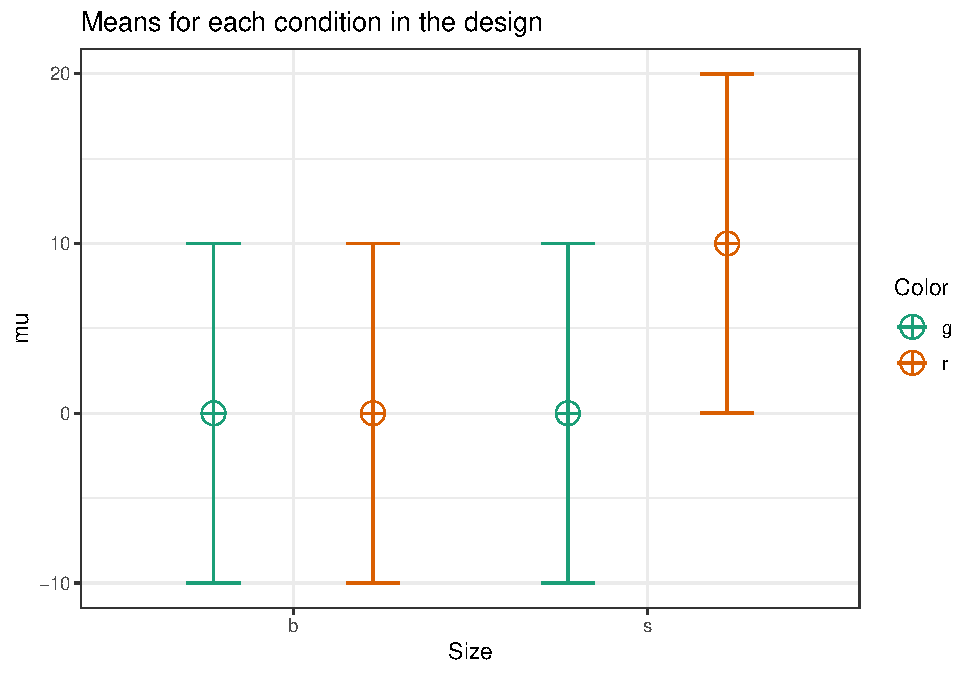
\includegraphics{SuperpowerValidation_files/figure-latex/unnamed-chunk-74-1.pdf}

\begin{Shaded}
\begin{Highlighting}[]
\NormalTok{alpha_level <-}\StringTok{ }\FloatTok{0.05} \CommentTok{#We set the alpha level at 0.05. }
\NormalTok{power_result <-}\StringTok{ }\KeywordTok{ANOVA_power}\NormalTok{(design_result, }\DataTypeTok{alpha_level =}\NormalTok{ alpha_level, }\DataTypeTok{nsims =}\NormalTok{ nsims)}
\end{Highlighting}
\end{Shaded}

\begin{verbatim}
## Power and Effect sizes for ANOVA tests
##                    power effect_size
## anova_fruit           33    0.005426
## anova_hunger          38    0.006345
## anova_fruit:hunger    30    0.005728
## 
## Power and Effect sizes for contrasts
##                                                                  power
## p_fruit_apple_hunger_no hunger_fruit_apple_hunger_very hungry        5
## p_fruit_apple_hunger_no hunger_fruit_banana_hunger_no hunger         6
## p_fruit_apple_hunger_no hunger_fruit_banana_hunger_very hungry      53
## p_fruit_apple_hunger_very hungry_fruit_banana_hunger_no hunger       5
## p_fruit_apple_hunger_very hungry_fruit_banana_hunger_very hungry    63
## p_fruit_banana_hunger_no hunger_fruit_banana_hunger_very hungry     69
##                                                                  effect_size
## p_fruit_apple_hunger_no hunger_fruit_apple_hunger_very hungry       0.007274
## p_fruit_apple_hunger_no hunger_fruit_banana_hunger_no hunger       -0.009399
## p_fruit_apple_hunger_no hunger_fruit_banana_hunger_very hungry      0.256463
## p_fruit_apple_hunger_very hungry_fruit_banana_hunger_no hunger     -0.016857
## p_fruit_apple_hunger_very hungry_fruit_banana_hunger_very hungry    0.249103
## p_fruit_banana_hunger_no hunger_fruit_banana_hunger_very hungry     0.266276
\end{verbatim}

And changing the sample size to 300 should reproduce the power for the interaction in the ANOVA.

\begin{Shaded}
\begin{Highlighting}[]
\NormalTok{string <-}\StringTok{ "2b*2b"}
\NormalTok{n <-}\StringTok{ }\DecValTok{300}
\NormalTok{mu <-}\StringTok{ }\KeywordTok{c}\NormalTok{(}\DecValTok{20}\NormalTok{, }\DecValTok{20}\NormalTok{, }\DecValTok{20}\NormalTok{, }\DecValTok{25}\NormalTok{) }\CommentTok{#All means are equal - so there is no real difference.}
\CommentTok{# Enter means in the order that matches the labels below.}
\NormalTok{sd <-}\StringTok{ }\DecValTok{20}
\NormalTok{labelnames <-}\StringTok{ }\KeywordTok{c}\NormalTok{(}\StringTok{"fruit"}\NormalTok{, }\StringTok{"apple"}\NormalTok{, }\StringTok{"banana"}\NormalTok{, }\StringTok{"hunger"}\NormalTok{, }\StringTok{"no hunger"}\NormalTok{, }\StringTok{"very hungry"}\NormalTok{) }\CommentTok{#}
\CommentTok{# the label names should be in the order of the means specified above.}
\NormalTok{design_result <-}\StringTok{ }\KeywordTok{ANOVA_design}\NormalTok{(}\DataTypeTok{design =}\NormalTok{ string,}
                   \DataTypeTok{n =}\NormalTok{ n, }
                   \DataTypeTok{mu =}\NormalTok{ mu, }
                   \DataTypeTok{sd =}\NormalTok{ sd, }
                   \DataTypeTok{labelnames =}\NormalTok{ labelnames)}
\end{Highlighting}
\end{Shaded}

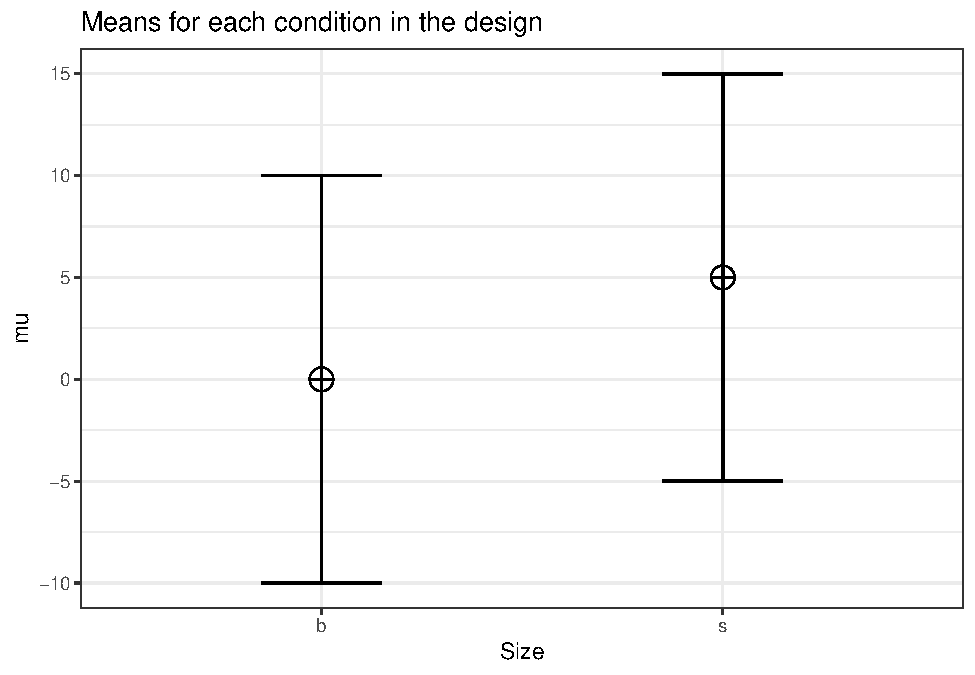
\includegraphics{SuperpowerValidation_files/figure-latex/unnamed-chunk-75-1.pdf}

\begin{Shaded}
\begin{Highlighting}[]
\NormalTok{alpha_level <-}\StringTok{ }\FloatTok{0.05} \CommentTok{#We set the alpha level at 0.05. }
\NormalTok{power_result <-}\StringTok{ }\KeywordTok{ANOVA_power}\NormalTok{(design_result, }\DataTypeTok{alpha_level =}\NormalTok{ alpha_level, }\DataTypeTok{nsims =}\NormalTok{ nsims)}
\end{Highlighting}
\end{Shaded}

\begin{verbatim}
## Power and Effect sizes for ANOVA tests
##                    power effect_size
## anova_fruit           63    0.004449
## anova_hunger          64    0.005619
## anova_fruit:hunger    53    0.004759
## 
## Power and Effect sizes for contrasts
##                                                                  power
## p_fruit_apple_hunger_no hunger_fruit_apple_hunger_very hungry        8
## p_fruit_apple_hunger_no hunger_fruit_banana_hunger_no hunger         4
## p_fruit_apple_hunger_no hunger_fruit_banana_hunger_very hungry      86
## p_fruit_apple_hunger_very hungry_fruit_banana_hunger_no hunger       7
## p_fruit_apple_hunger_very hungry_fruit_banana_hunger_very hungry    86
## p_fruit_banana_hunger_no hunger_fruit_banana_hunger_very hungry     89
##                                                                  effect_size
## p_fruit_apple_hunger_no hunger_fruit_apple_hunger_very hungry       0.010926
## p_fruit_apple_hunger_no hunger_fruit_banana_hunger_no hunger       -0.002831
## p_fruit_apple_hunger_no hunger_fruit_banana_hunger_very hungry      0.258490
## p_fruit_apple_hunger_very hungry_fruit_banana_hunger_no hunger     -0.013783
## p_fruit_apple_hunger_very hungry_fruit_banana_hunger_very hungry    0.246630
## p_fruit_banana_hunger_no hunger_fruit_banana_hunger_very hungry     0.261495
\end{verbatim}

Now if we look at the power analysis table for the last simulation, we see that the power for the ANOVA is the same for the main effect of fruit, the main effect of hunger, and the main effect of the interaction. All the effect sizes are equal as well. We can understand why if we look at the means in a 2x2 table:

\begin{Shaded}
\begin{Highlighting}[]
\NormalTok{mean_mat <-}\StringTok{ }\KeywordTok{t}\NormalTok{(}\KeywordTok{matrix}\NormalTok{(mu, }
                     \DataTypeTok{nrow =} \DecValTok{2}\NormalTok{,}
                     \DataTypeTok{ncol =} \DecValTok{2}\NormalTok{)) }\CommentTok{#Create a mean matrix}
\KeywordTok{rownames}\NormalTok{(mean_mat) <-}\StringTok{ }\KeywordTok{c}\NormalTok{(}\StringTok{"apple"}\NormalTok{, }\StringTok{"banana"}\NormalTok{)}
\KeywordTok{colnames}\NormalTok{(mean_mat) <-}\StringTok{ }\KeywordTok{c}\NormalTok{(}\StringTok{"no hunger"}\NormalTok{, }\StringTok{"very hungry"}\NormalTok{)}
\NormalTok{mean_mat}
\end{Highlighting}
\end{Shaded}

\begin{verbatim}
##        no hunger very hungry
## apple         20          20
## banana        20          25
\end{verbatim}

The first main effect tests the marginal means if we sum over rows, 22.5 vs 20.

\begin{Shaded}
\begin{Highlighting}[]
\KeywordTok{rowMeans}\NormalTok{(mean_mat)}
\end{Highlighting}
\end{Shaded}

\begin{verbatim}
##  apple banana 
##   20.0   22.5
\end{verbatim}

The second main effect tests the marginal means over the rows, which is also 22.5 vs 20.

\begin{Shaded}
\begin{Highlighting}[]
\KeywordTok{colMeans}\NormalTok{(mean_mat)}
\end{Highlighting}
\end{Shaded}

\begin{verbatim}
##   no hunger very hungry 
##        20.0        22.5
\end{verbatim}

The interaction tests whether the average effect of hunger on liking fruit differs in the presence of bananas. In the presence of bananas the effect of hunger on the desireability of fruit is 5 scalepoints. The average effect (that we get from the marginal means) of hunger on fruit desireability is 2.5 (22.5-20). In other words, the interaction tests whether the difference effect between hunger and no hunger is different in the presence of an apple versus in the presence of a banana.

Mathematically the interaction effect is computed as the difference between a cell mean and the grand mean, the marginal mean in row i and the grand mean, and the marginal mean in column j and grand mean. For example, for the very hungry-banana condition this is 25 (the value in the cell) - (21.25 {[}the grand mean{]} + 1.25 {[}the marginal mean in row 2, 22.5, minus the grand mean of 21.25{]} + 1.25 {[}the marginal mean in column 2, 22.5, minus the grand mean of 21.25{]}). 25 - (21.25 + (22.5-21.25) + (22.5-21.25)) = 1.25.

We can repeat this for every cell, and get for no hunger-apple: 20 - (21.25 + (20-21.25) + (20-21.25)) = 1.25, for very hungry apple: 20 - (21.25 + (22.5-21.25) + (20-21.25)) = 1.25, and no hunger-banana: 20 - (21.25 + (20-21.25) + (22.5-21.25)) = 1.25. These values are used to calculate the sum of squares.

\begin{Shaded}
\begin{Highlighting}[]
\NormalTok{a1 <-}\StringTok{ }\NormalTok{mean_mat[}\DecValTok{1}\NormalTok{,}\DecValTok{1}\NormalTok{] }\OperatorTok{-}\StringTok{ }\NormalTok{(}\KeywordTok{mean}\NormalTok{(mean_mat) }\OperatorTok{+}\StringTok{ }\NormalTok{(}\KeywordTok{mean}\NormalTok{(mean_mat[}\DecValTok{1}\NormalTok{,]) }\OperatorTok{-}\StringTok{ }\KeywordTok{mean}\NormalTok{(mean_mat)) }\OperatorTok{+}\StringTok{ }\NormalTok{(}\KeywordTok{mean}\NormalTok{(mean_mat[,}\DecValTok{1}\NormalTok{]) }\OperatorTok{-}\StringTok{ }\KeywordTok{mean}\NormalTok{(mean_mat)))}
\NormalTok{a2 <-}\StringTok{ }\NormalTok{mean_mat[}\DecValTok{1}\NormalTok{,}\DecValTok{2}\NormalTok{] }\OperatorTok{-}\StringTok{ }\NormalTok{(}\KeywordTok{mean}\NormalTok{(mean_mat) }\OperatorTok{+}\StringTok{ }\NormalTok{(}\KeywordTok{mean}\NormalTok{(mean_mat[}\DecValTok{1}\NormalTok{,]) }\OperatorTok{-}\StringTok{ }\KeywordTok{mean}\NormalTok{(mean_mat)) }\OperatorTok{+}\StringTok{ }\NormalTok{(}\KeywordTok{mean}\NormalTok{(mean_mat[,}\DecValTok{2}\NormalTok{]) }\OperatorTok{-}\StringTok{ }\KeywordTok{mean}\NormalTok{(mean_mat)))}
\NormalTok{b1 <-}\StringTok{ }\NormalTok{mean_mat[}\DecValTok{2}\NormalTok{,}\DecValTok{1}\NormalTok{] }\OperatorTok{-}\StringTok{ }\NormalTok{(}\KeywordTok{mean}\NormalTok{(mean_mat) }\OperatorTok{+}\StringTok{ }\NormalTok{(}\KeywordTok{mean}\NormalTok{(mean_mat[}\DecValTok{2}\NormalTok{,]) }\OperatorTok{-}\StringTok{ }\KeywordTok{mean}\NormalTok{(mean_mat)) }\OperatorTok{+}\StringTok{ }\NormalTok{(}\KeywordTok{mean}\NormalTok{(mean_mat[,}\DecValTok{1}\NormalTok{]) }\OperatorTok{-}\StringTok{ }\KeywordTok{mean}\NormalTok{(mean_mat)))}
\NormalTok{b2 <-}\StringTok{ }\NormalTok{mean_mat[}\DecValTok{2}\NormalTok{,}\DecValTok{2}\NormalTok{] }\OperatorTok{-}\StringTok{ }\NormalTok{(}\KeywordTok{mean}\NormalTok{(mean_mat) }\OperatorTok{+}\StringTok{ }\NormalTok{(}\KeywordTok{mean}\NormalTok{(mean_mat[}\DecValTok{2}\NormalTok{,]) }\OperatorTok{-}\StringTok{ }\KeywordTok{mean}\NormalTok{(mean_mat)) }\OperatorTok{+}\StringTok{ }\NormalTok{(}\KeywordTok{mean}\NormalTok{(mean_mat[,}\DecValTok{2}\NormalTok{]) }\OperatorTok{-}\StringTok{ }\KeywordTok{mean}\NormalTok{(mean_mat)))}
\NormalTok{SS_ab <-}\StringTok{ }\NormalTok{n }\OperatorTok{*}\StringTok{ }\KeywordTok{sum}\NormalTok{(}\KeywordTok{c}\NormalTok{(a1, a2, b1, b2)}\OperatorTok{^}\DecValTok{2}\NormalTok{)}
\end{Highlighting}
\end{Shaded}

The sum of squares is dependent on the sample size, as can be seen in the code above. The larger the sample size, the larger the sum of squares, and therefore (all else equal) the larger the \emph{F}-statistic, and the smaller the \emph{p}-value. We see from the simulations that all three tests have the same effect size, and therefore the same power.

Interactions can have more power than main effects if the effect size of the interaction is larger than the effect size of the main effects. An example of this is a cross-over interaction. For example, let's take a 2x2 matrix of means with a crossover interaction:

\begin{Shaded}
\begin{Highlighting}[]
\NormalTok{mu <-}\StringTok{ }\KeywordTok{c}\NormalTok{(}\DecValTok{25}\NormalTok{, }\DecValTok{20}\NormalTok{, }\DecValTok{20}\NormalTok{, }\DecValTok{25}\NormalTok{)}
\NormalTok{mean_mat <-}\StringTok{ }\KeywordTok{t}\NormalTok{(}\KeywordTok{matrix}\NormalTok{(mu, }
                     \DataTypeTok{nrow =} \DecValTok{2}\NormalTok{,}
                     \DataTypeTok{ncol =} \DecValTok{2}\NormalTok{)) }\CommentTok{#Create a mean matrix}
\KeywordTok{rownames}\NormalTok{(mean_mat) <-}\StringTok{ }\KeywordTok{c}\NormalTok{(}\StringTok{"apple"}\NormalTok{, }\StringTok{"banana"}\NormalTok{)}
\KeywordTok{colnames}\NormalTok{(mean_mat) <-}\StringTok{ }\KeywordTok{c}\NormalTok{(}\StringTok{"no hunger"}\NormalTok{, }\StringTok{"very hungry"}\NormalTok{)}
\NormalTok{mean_mat}
\end{Highlighting}
\end{Shaded}

\begin{verbatim}
##        no hunger very hungry
## apple         25          20
## banana        20          25
\end{verbatim}

Neither of the main effects is now significant, as the marginal means are 22.5 vs 22.5 for both main effects. The interaction is much stronger, however. We are testing whether the average effect of hunger on the desireability of fruit is different in the presence of bananas. Since the average effect is 0, and the effect of hunger on the desireability of bananas is 5, so the effect size is now twice as large.

\begin{Shaded}
\begin{Highlighting}[]
\NormalTok{string <-}\StringTok{ "2b*2b"}
\NormalTok{n <-}\StringTok{ }\DecValTok{300}
\NormalTok{mu <-}\StringTok{ }\KeywordTok{c}\NormalTok{(}\DecValTok{25}\NormalTok{, }\DecValTok{20}\NormalTok{, }\DecValTok{20}\NormalTok{, }\DecValTok{25}\NormalTok{) }\CommentTok{#All means are equal - so there is no real difference.}
\CommentTok{# Enter means in the order that matches the labels below.}
\NormalTok{sd <-}\StringTok{ }\DecValTok{20}
\NormalTok{labelnames <-}\StringTok{ }\KeywordTok{c}\NormalTok{(}\StringTok{"fruit"}\NormalTok{, }\StringTok{"apple"}\NormalTok{, }\StringTok{"banana"}\NormalTok{, }\StringTok{"hunger"}\NormalTok{, }\StringTok{"no hunger"}\NormalTok{, }\StringTok{"very hungry"}\NormalTok{) }\CommentTok{#}
\CommentTok{# the label names should be in the order of the means specified above.}
\NormalTok{design_result <-}\StringTok{ }\KeywordTok{ANOVA_design}\NormalTok{(}\DataTypeTok{design =}\NormalTok{ string,}
                   \DataTypeTok{n =}\NormalTok{ n, }
                   \DataTypeTok{mu =}\NormalTok{ mu, }
                   \DataTypeTok{sd =}\NormalTok{ sd, }
                   \DataTypeTok{labelnames =}\NormalTok{ labelnames)}
\end{Highlighting}
\end{Shaded}

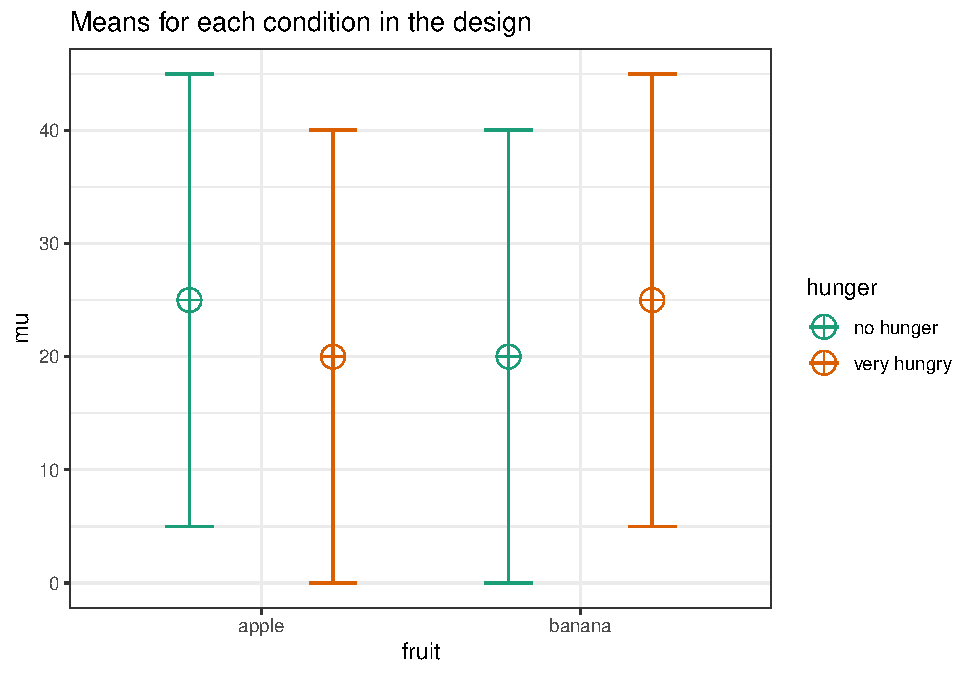
\includegraphics{SuperpowerValidation_files/figure-latex/unnamed-chunk-81-1.pdf}

\begin{Shaded}
\begin{Highlighting}[]
\NormalTok{alpha_level <-}\StringTok{ }\FloatTok{0.05} \CommentTok{#We set the alpha level at 0.05. }
\NormalTok{power_result <-}\StringTok{ }\KeywordTok{ANOVA_power}\NormalTok{(design_result, }\DataTypeTok{alpha_level =}\NormalTok{ alpha_level, }\DataTypeTok{nsims =}\NormalTok{ nsims)}
\end{Highlighting}
\end{Shaded}

\begin{verbatim}
## Power and Effect sizes for ANOVA tests
##                    power effect_size
## anova_fruit            5   0.0009895
## anova_hunger           6   0.0006749
## anova_fruit:hunger    99   0.0166921
## 
## Power and Effect sizes for contrasts
##                                                                  power
## p_fruit_apple_hunger_no hunger_fruit_apple_hunger_very hungry       90
## p_fruit_apple_hunger_no hunger_fruit_banana_hunger_no hunger        87
## p_fruit_apple_hunger_no hunger_fruit_banana_hunger_very hungry       8
## p_fruit_apple_hunger_very hungry_fruit_banana_hunger_no hunger       5
## p_fruit_apple_hunger_very hungry_fruit_banana_hunger_very hungry    84
## p_fruit_banana_hunger_no hunger_fruit_banana_hunger_very hungry     90
##                                                                  effect_size
## p_fruit_apple_hunger_no hunger_fruit_apple_hunger_very hungry     -0.2516739
## p_fruit_apple_hunger_no hunger_fruit_banana_hunger_no hunger      -0.2552283
## p_fruit_apple_hunger_no hunger_fruit_banana_hunger_very hungry     0.0008431
## p_fruit_apple_hunger_very hungry_fruit_banana_hunger_no hunger    -0.0041340
## p_fruit_apple_hunger_very hungry_fruit_banana_hunger_very hungry   0.2532954
## p_fruit_banana_hunger_no hunger_fruit_banana_hunger_very hungry    0.2570198
\end{verbatim}

We can also reproduce the power analysis using the anlytic function:

\begin{Shaded}
\begin{Highlighting}[]
\NormalTok{power_analytic <-}\StringTok{ }\KeywordTok{power_twoway_between}\NormalTok{(design_result)}
\NormalTok{power_analytic}\OperatorTok{$}\NormalTok{power_A}
\end{Highlighting}
\end{Shaded}

\begin{verbatim}
## [1] 0.05
\end{verbatim}

\begin{Shaded}
\begin{Highlighting}[]
\NormalTok{power_analytic}\OperatorTok{$}\NormalTok{power_B}
\end{Highlighting}
\end{Shaded}

\begin{verbatim}
## [1] 0.05
\end{verbatim}

\hypertarget{analytic-power-functions}{%
\chapter{Analytic Power Functions}\label{analytic-power-functions}}

For some designs it is possible to calculate power analytically, using closed functions.

\hypertarget{one-way-between-subject-anova}{%
\section{One-Way Between Subject ANOVA}\label{one-way-between-subject-anova}}

\begin{Shaded}
\begin{Highlighting}[]
\NormalTok{string <-}\StringTok{ "4b"}
\NormalTok{n <-}\StringTok{ }\DecValTok{60}
\NormalTok{mu <-}\StringTok{ }\KeywordTok{c}\NormalTok{(}\DecValTok{80}\NormalTok{, }\DecValTok{82}\NormalTok{, }\DecValTok{82}\NormalTok{, }\DecValTok{86}\NormalTok{) }\CommentTok{#All means are equal - so there is no real difference.}
\CommentTok{# Enter means in the order that matches the labels below.}
\NormalTok{sd <-}\StringTok{ }\DecValTok{10}
\NormalTok{labelnames <-}\StringTok{ }\KeywordTok{c}\NormalTok{(}\StringTok{"Factor_A"}\NormalTok{, }\StringTok{"a1"}\NormalTok{, }\StringTok{"a2"}\NormalTok{, }\StringTok{"a3"}\NormalTok{, }\StringTok{"a4"}\NormalTok{) }\CommentTok{#}
\CommentTok{# the label names should be in the order of the means specified above.}
\NormalTok{design_result <-}\StringTok{ }\KeywordTok{ANOVA_design}\NormalTok{(}\DataTypeTok{design =}\NormalTok{ string,}
                   \DataTypeTok{n =}\NormalTok{ n, }
                   \DataTypeTok{mu =}\NormalTok{ mu, }
                   \DataTypeTok{sd =}\NormalTok{ sd, }
                   \DataTypeTok{labelnames =}\NormalTok{ labelnames)}
\end{Highlighting}
\end{Shaded}

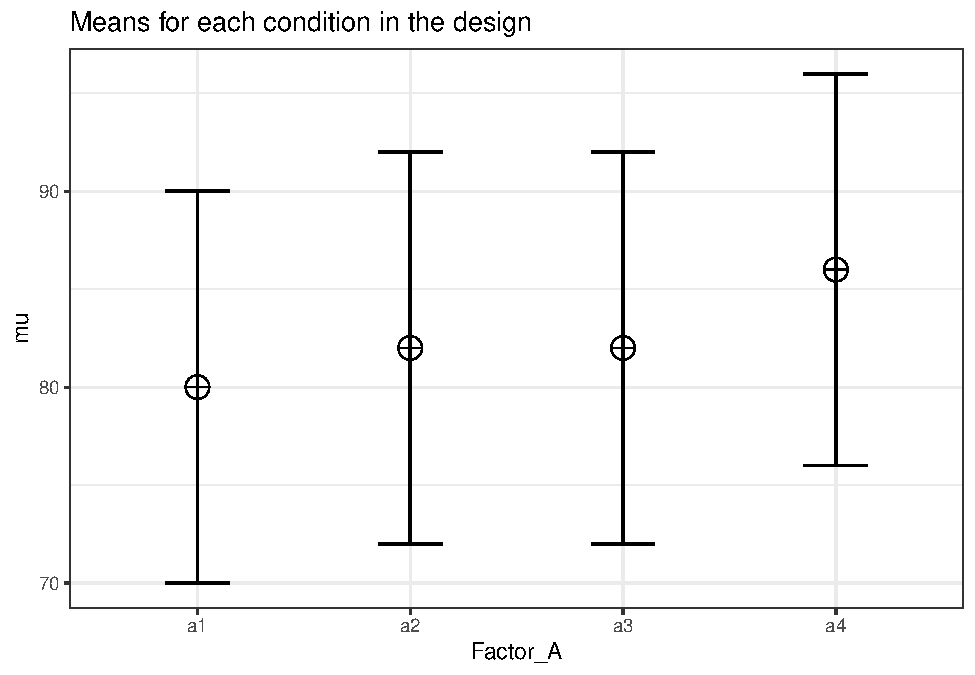
\includegraphics{SuperpowerValidation_files/figure-latex/unnamed-chunk-83-1.pdf}

\begin{Shaded}
\begin{Highlighting}[]
\NormalTok{power_result <-}\StringTok{ }\KeywordTok{ANOVA_power}\NormalTok{(design_result, }\DataTypeTok{alpha_level =} \FloatTok{0.05}\NormalTok{, }\DataTypeTok{nsims =}\NormalTok{ nsims)}
\end{Highlighting}
\end{Shaded}

\begin{verbatim}
## Power and Effect sizes for ANOVA tests
##                power effect_size
## anova_Factor_A    84     0.05683
## 
## Power and Effect sizes for contrasts
##                           power effect_size
## p_Factor_A_a1_Factor_A_a2    21    0.218427
## p_Factor_A_a1_Factor_A_a3    20    0.227226
## p_Factor_A_a1_Factor_A_a4    92    0.608481
## p_Factor_A_a2_Factor_A_a3     6    0.007324
## p_Factor_A_a2_Factor_A_a4    52    0.391843
## p_Factor_A_a3_Factor_A_a4    51    0.382210
\end{verbatim}

We can also calculate power analytically with our own function.

\begin{Shaded}
\begin{Highlighting}[]
\KeywordTok{power_oneway_between}\NormalTok{(design_result)}\OperatorTok{$}\NormalTok{power }\CommentTok{#using default alpha level of .05}
\end{Highlighting}
\end{Shaded}

\begin{verbatim}
## [1] 0.8121291
\end{verbatim}

This is a generalized function for One-Way ANOVA's for any number of groups. It is in part based on code provided with the excellent book by Aberson (2019) Applied Power Analysis for the Behavioral Sciences (but Aberson's code allows for different n per condition, and different sd per condition).

\begin{Shaded}
\begin{Highlighting}[]
\KeywordTok{anova1f_4}\NormalTok{(}\DataTypeTok{m1 =} \DecValTok{80}\NormalTok{, }\DataTypeTok{m2 =} \DecValTok{82}\NormalTok{, }\DataTypeTok{m3 =} \DecValTok{82}\NormalTok{, }\DataTypeTok{m4 =} \DecValTok{86}\NormalTok{,}
          \DataTypeTok{s1 =} \DecValTok{10}\NormalTok{, }\DataTypeTok{s2 =} \DecValTok{10}\NormalTok{, }\DataTypeTok{s3 =} \DecValTok{10}\NormalTok{, }\DataTypeTok{s4 =} \DecValTok{10}\NormalTok{,}
          \DataTypeTok{n1 =} \DecValTok{60}\NormalTok{, }\DataTypeTok{n2 =} \DecValTok{60}\NormalTok{, }\DataTypeTok{n3 =} \DecValTok{60}\NormalTok{, }\DataTypeTok{n4 =} \DecValTok{60}\NormalTok{,}
          \DataTypeTok{alpha =} \FloatTok{.05}\NormalTok{)}
\end{Highlighting}
\end{Shaded}

We can also use the function in the pwr package. Note that we need to calculate f to use this function, which is based on the means and sd, as illustrated in the formulas above.

\begin{Shaded}
\begin{Highlighting}[]
\KeywordTok{pwr.anova.test}\NormalTok{(}\DataTypeTok{n =} \DecValTok{60}\NormalTok{,}
               \DataTypeTok{k =} \DecValTok{4}\NormalTok{,}
               \DataTypeTok{f =} \FloatTok{0.2179449}\NormalTok{,}
               \DataTypeTok{sig.level =} \FloatTok{0.05}\NormalTok{)}
\end{Highlighting}
\end{Shaded}

\begin{verbatim}
## 
##      Balanced one-way analysis of variance power calculation 
## 
##               k = 4
##               n = 60
##               f = 0.2179449
##       sig.level = 0.05
##           power = 0.8121289
## 
## NOTE: n is number in each group
\end{verbatim}

Finally, G*Power provides the option to calculate f from the means, sd and n for the cells. It can then be used to calculate power.

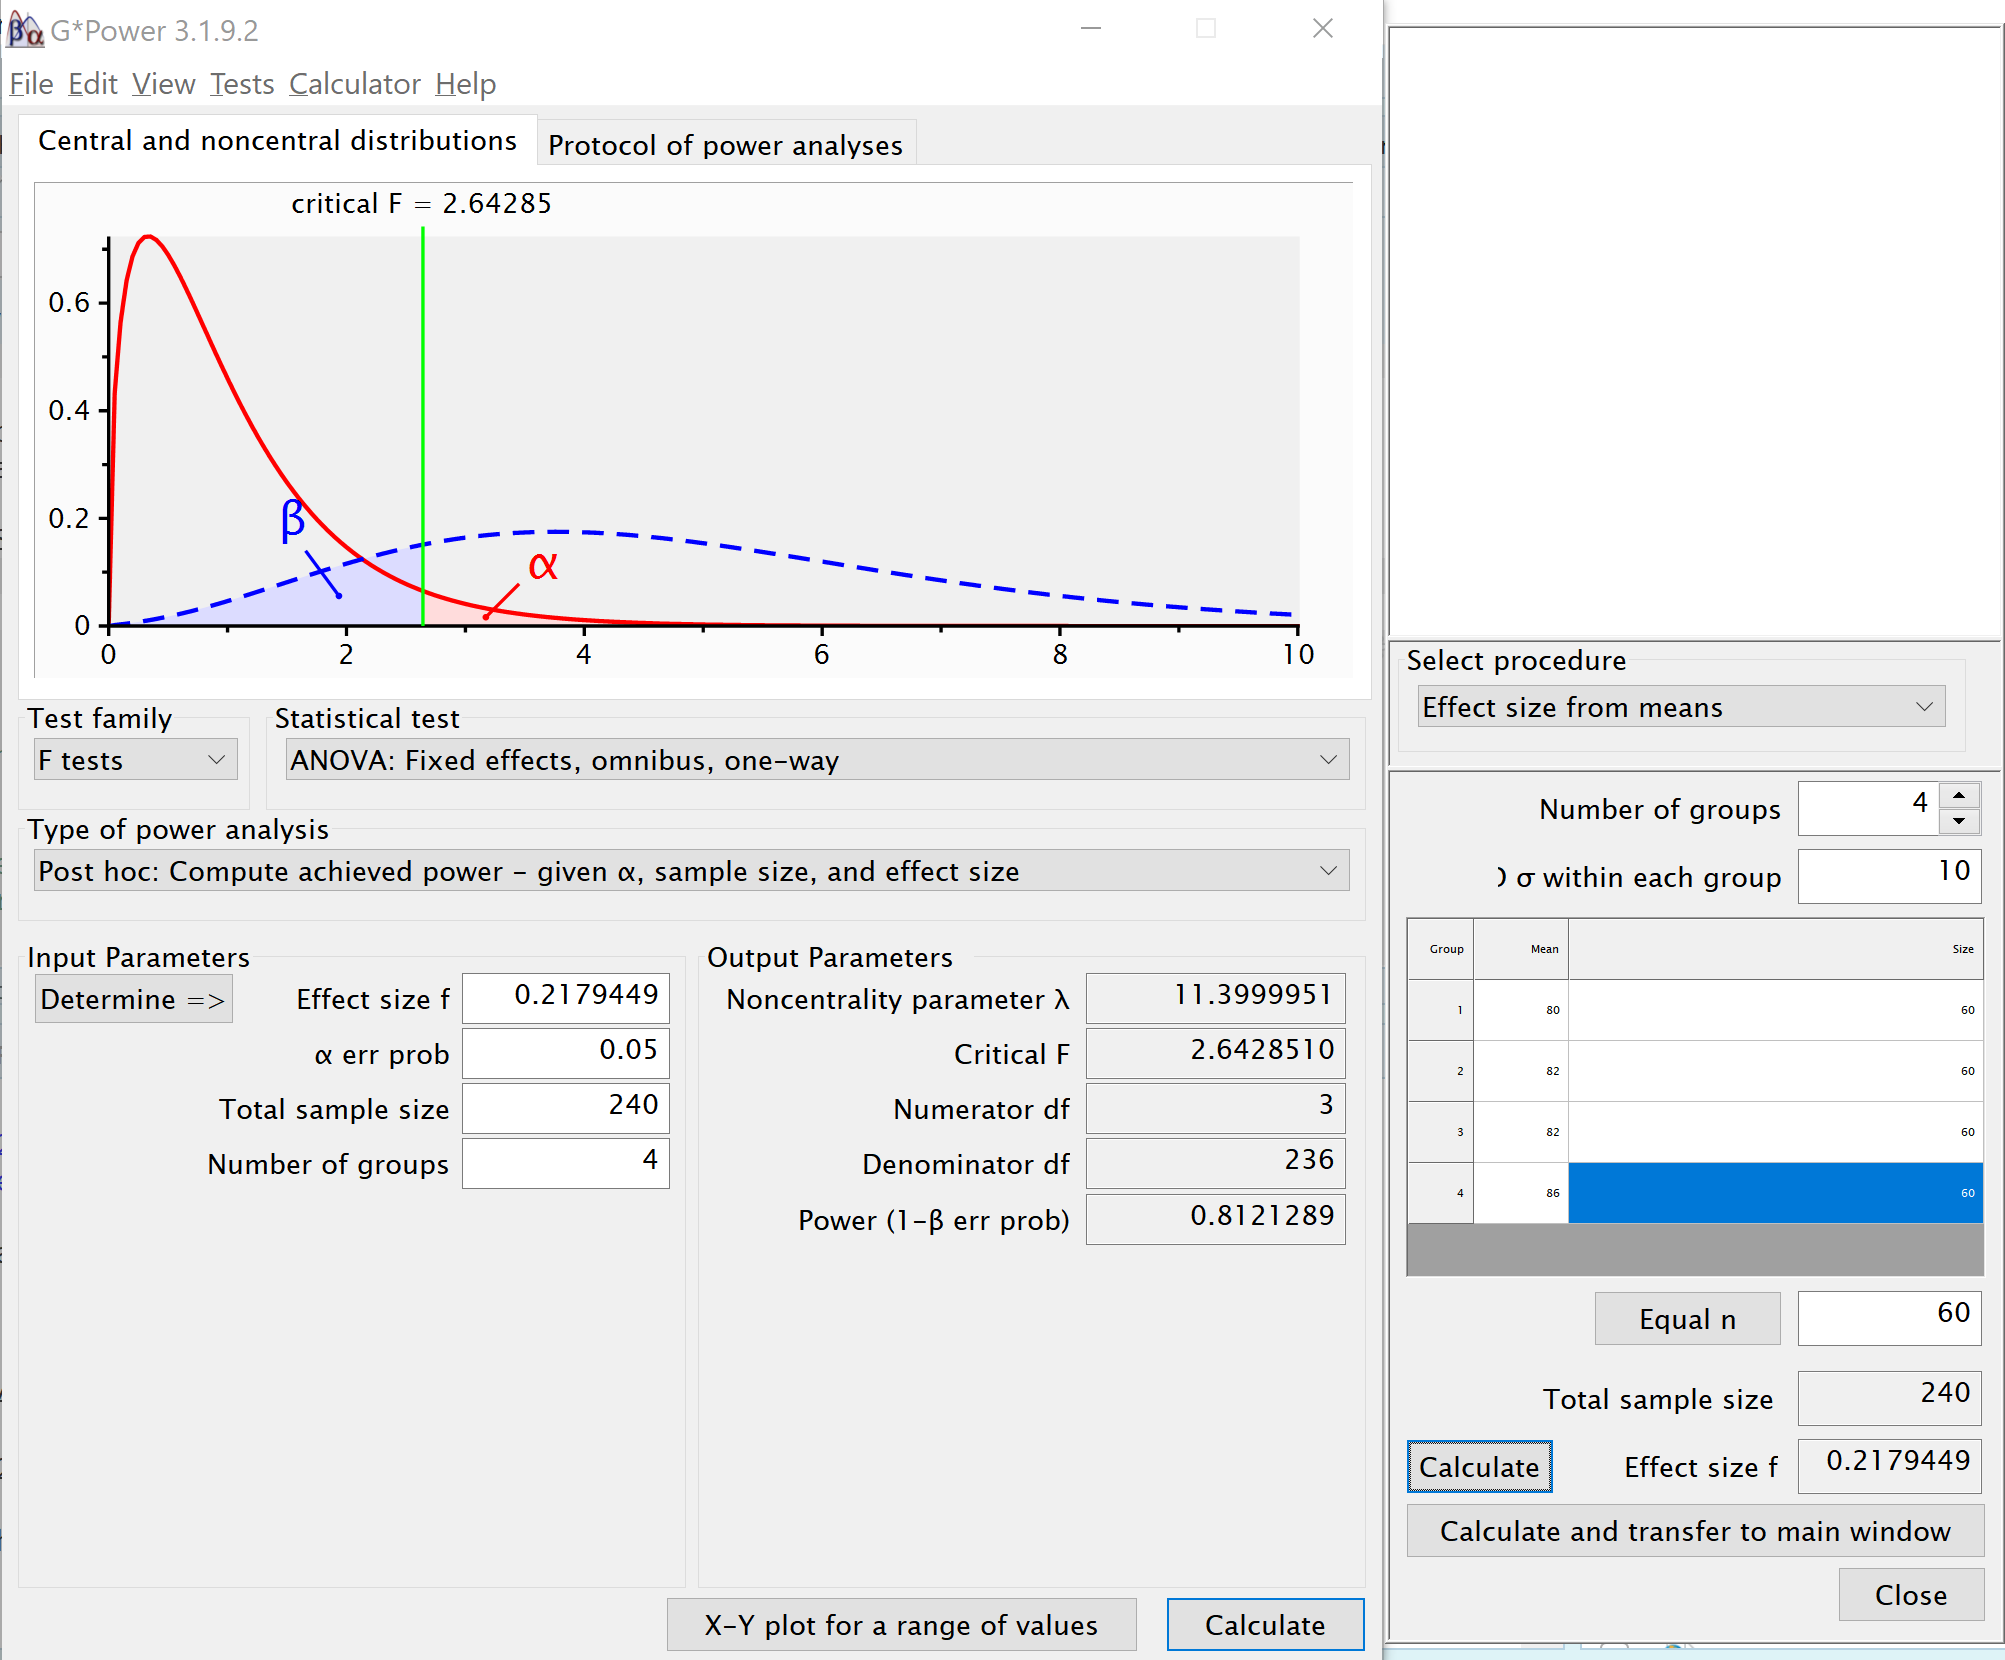
\includegraphics{screenshots/gpower_13.png}

\hypertarget{two-way-between-subject-interaction}{%
\section{Two-way Between Subject Interaction}\label{two-way-between-subject-interaction}}

\begin{Shaded}
\begin{Highlighting}[]
\NormalTok{string <-}\StringTok{ "2b*2b"}
\NormalTok{n <-}\StringTok{ }\DecValTok{20}
\NormalTok{mu <-}\StringTok{ }\KeywordTok{c}\NormalTok{(}\DecValTok{20}\NormalTok{, }\DecValTok{20}\NormalTok{, }\DecValTok{20}\NormalTok{, }\DecValTok{25}\NormalTok{) }
\CommentTok{# Enter means in the order that matches the labels below.}
\NormalTok{sd <-}\StringTok{ }\DecValTok{5}
\NormalTok{labelnames <-}\StringTok{ }\KeywordTok{c}\NormalTok{(}\StringTok{"A"}\NormalTok{, }\StringTok{"a1"}\NormalTok{, }\StringTok{"a2"}\NormalTok{, }\StringTok{"B"}\NormalTok{, }\StringTok{"b1"}\NormalTok{, }\StringTok{"b2"}\NormalTok{) }\CommentTok{#}
\CommentTok{# the label names should be in the order of the means specified above.}
\NormalTok{design_result <-}\StringTok{ }\KeywordTok{ANOVA_design}\NormalTok{(}\DataTypeTok{design =}\NormalTok{ string,}
                   \DataTypeTok{n =}\NormalTok{ n, }
                   \DataTypeTok{mu =}\NormalTok{ mu, }
                   \DataTypeTok{sd =}\NormalTok{ sd, }
                   \DataTypeTok{labelnames =}\NormalTok{ labelnames)}
\end{Highlighting}
\end{Shaded}

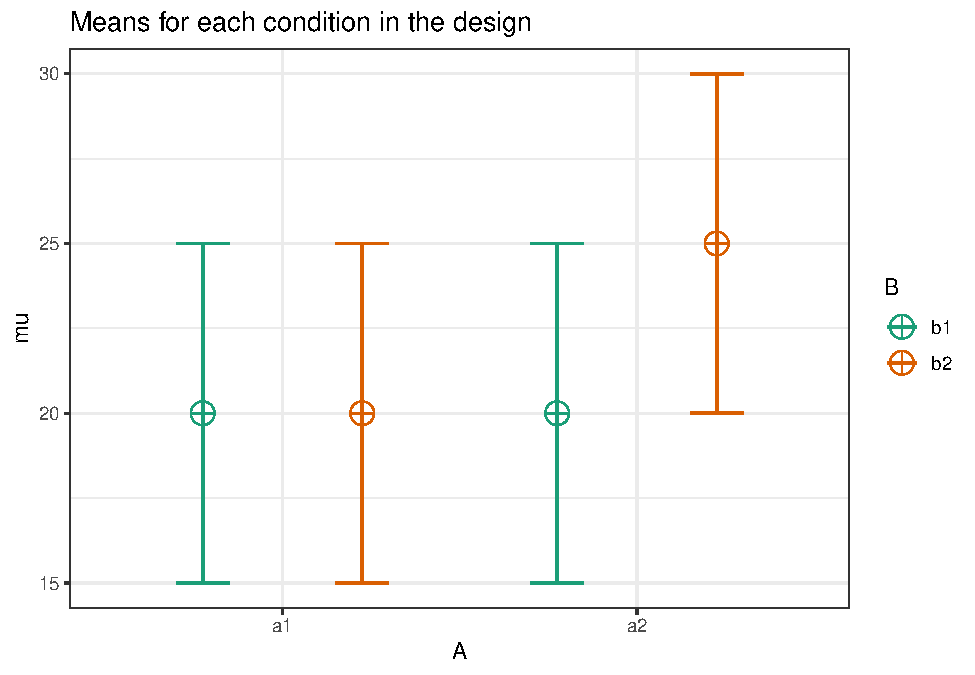
\includegraphics{SuperpowerValidation_files/figure-latex/unnamed-chunk-87-1.pdf}

\begin{Shaded}
\begin{Highlighting}[]
\NormalTok{power_result <-}\StringTok{ }\KeywordTok{ANOVA_power}\NormalTok{(design_result, }\DataTypeTok{alpha_level =} \FloatTok{0.05}\NormalTok{, }\DataTypeTok{nsims =}\NormalTok{ nsims)}
\end{Highlighting}
\end{Shaded}

\begin{verbatim}
## Power and Effect sizes for ANOVA tests
##           power effect_size
## anova_A      65     0.08011
## anova_B      61     0.07314
## anova_A:B    60     0.06963
## 
## Power and Effect sizes for contrasts
##                       power effect_size
## p_A_a1_B_b1_A_a1_B_b2     6     0.01091
## p_A_a1_B_b1_A_a2_B_b1     4     0.04024
## p_A_a1_B_b1_A_a2_B_b2    88     1.06041
## p_A_a1_B_b2_A_a2_B_b1     4     0.02876
## p_A_a1_B_b2_A_a2_B_b2    88     1.03465
## p_A_a2_B_b1_A_a2_B_b2    87     1.00829
\end{verbatim}

\begin{Shaded}
\begin{Highlighting}[]
\NormalTok{power_res <-}\StringTok{ }\KeywordTok{power_twoway_between}\NormalTok{(design_result) }\CommentTok{#using default alpha level of .05}
\NormalTok{power_res}\OperatorTok{$}\NormalTok{power_A}
\end{Highlighting}
\end{Shaded}

\begin{verbatim}
## [1] 0.5978655
\end{verbatim}

\begin{Shaded}
\begin{Highlighting}[]
\NormalTok{power_res}\OperatorTok{$}\NormalTok{power_B}
\end{Highlighting}
\end{Shaded}

\begin{verbatim}
## [1] 0.5978655
\end{verbatim}

\begin{Shaded}
\begin{Highlighting}[]
\NormalTok{power_res}\OperatorTok{$}\NormalTok{power_AB}
\end{Highlighting}
\end{Shaded}

\begin{verbatim}
## [1] 0.5978655
\end{verbatim}

We can use the function by Aberson, 2019, as well.

\begin{Shaded}
\begin{Highlighting}[]
\KeywordTok{anova2x2}\NormalTok{(}\DataTypeTok{m1.1=}\DecValTok{20}\NormalTok{,}
         \DataTypeTok{m1.2=}\DecValTok{20}\NormalTok{,}
         \DataTypeTok{m2.1=}\DecValTok{20}\NormalTok{,}
         \DataTypeTok{m2.2=}\DecValTok{25}\NormalTok{, }
         \DataTypeTok{s1.1=}\DecValTok{5}\NormalTok{,}
         \DataTypeTok{s1.2=}\DecValTok{5}\NormalTok{,}
         \DataTypeTok{s2.1=}\DecValTok{5}\NormalTok{,}
         \DataTypeTok{s2.2=}\DecValTok{5}\NormalTok{,}
         \DataTypeTok{n1.1=}\DecValTok{20}\NormalTok{,}
         \DataTypeTok{n1.2=}\DecValTok{20}\NormalTok{,}
         \DataTypeTok{n2.1=}\DecValTok{20}\NormalTok{,}
         \DataTypeTok{n2.2=}\DecValTok{20}\NormalTok{, }
         \DataTypeTok{alpha=}\NormalTok{.}\DecValTok{05}\NormalTok{, }
         \DataTypeTok{all=}\StringTok{"OFF"}\NormalTok{)}
\end{Highlighting}
\end{Shaded}

\hypertarget{x3-between-subject-anova}{%
\section{3x3 Between Subject ANOVA}\label{x3-between-subject-anova}}

\begin{Shaded}
\begin{Highlighting}[]
\NormalTok{string <-}\StringTok{ "3b*3b"}
\NormalTok{n <-}\StringTok{ }\DecValTok{20}
\NormalTok{mu <-}\StringTok{ }\KeywordTok{c}\NormalTok{(}\DecValTok{20}\NormalTok{, }\DecValTok{20}\NormalTok{, }\DecValTok{20}\NormalTok{, }\DecValTok{20}\NormalTok{, }\DecValTok{20}\NormalTok{, }\DecValTok{20}\NormalTok{, }\DecValTok{20}\NormalTok{, }\DecValTok{20}\NormalTok{, }\DecValTok{25}\NormalTok{) }\CommentTok{#All means are equal - so there is no real difference.}
\CommentTok{# Enter means in the order that matches the labels below.}
\NormalTok{sd <-}\StringTok{ }\DecValTok{5}
\NormalTok{labelnames <-}\StringTok{ }\KeywordTok{c}\NormalTok{(}\StringTok{"Factor_A"}\NormalTok{, }\StringTok{"a1"}\NormalTok{, }\StringTok{"a2"}\NormalTok{, }\StringTok{"a3"}\NormalTok{, }\StringTok{"Factor_B"}\NormalTok{, }\StringTok{"b1"}\NormalTok{, }\StringTok{"b2"}\NormalTok{, }\StringTok{"b3"}\NormalTok{) }\CommentTok{#}
\CommentTok{# the label names should be in the order of the means specified above.}
\NormalTok{design_result <-}\StringTok{ }\KeywordTok{ANOVA_design}\NormalTok{(}\DataTypeTok{design =}\NormalTok{ string,}
                   \DataTypeTok{n =}\NormalTok{ n, }
                   \DataTypeTok{mu =}\NormalTok{ mu, }
                   \DataTypeTok{sd =}\NormalTok{ sd, }
                   \DataTypeTok{labelnames =}\NormalTok{ labelnames)}
\end{Highlighting}
\end{Shaded}

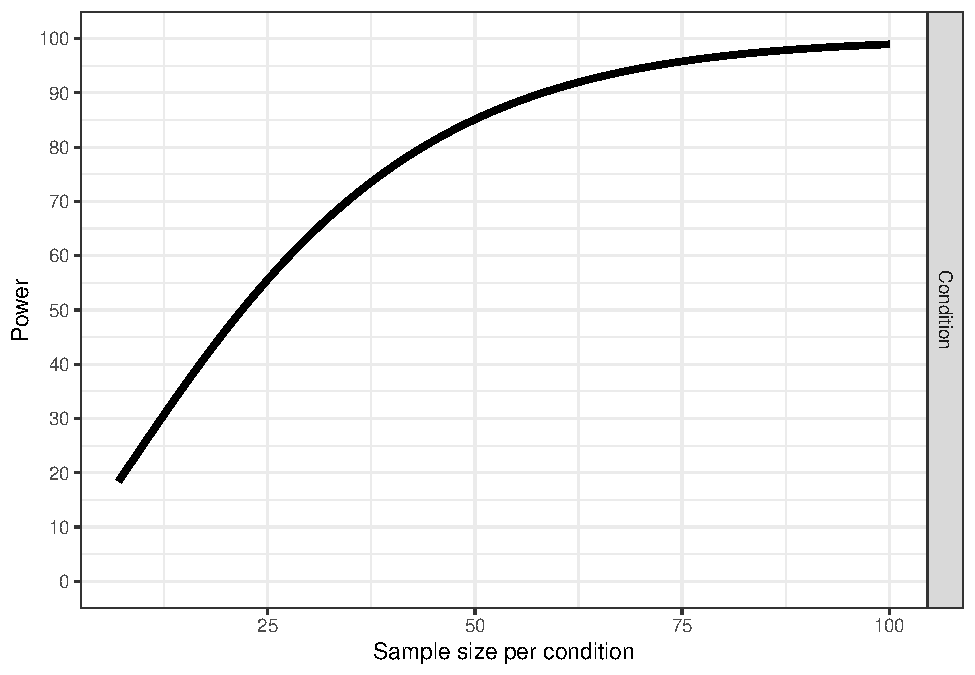
\includegraphics{SuperpowerValidation_files/figure-latex/unnamed-chunk-90-1.pdf}

\begin{Shaded}
\begin{Highlighting}[]
\NormalTok{power_result <-}\StringTok{ }\KeywordTok{ANOVA_power}\NormalTok{(design_result, }\DataTypeTok{alpha_level =} \FloatTok{0.05}\NormalTok{, }\DataTypeTok{nsims =}\NormalTok{ nsims)}
\end{Highlighting}
\end{Shaded}

\begin{verbatim}
## Power and Effect sizes for ANOVA tests
##                         power effect_size
## anova_Factor_A             40     0.03563
## anova_Factor_B             43     0.03753
## anova_Factor_A:Factor_B    61     0.06852
## 
## Power and Effect sizes for contrasts
##                                                   power effect_size
## p_Factor_A_a1_Factor_B_b1_Factor_A_a1_Factor_B_b2     6  -0.0024935
## p_Factor_A_a1_Factor_B_b1_Factor_A_a1_Factor_B_b3     3   0.0484236
## p_Factor_A_a1_Factor_B_b1_Factor_A_a2_Factor_B_b1     5   0.0123203
## p_Factor_A_a1_Factor_B_b1_Factor_A_a2_Factor_B_b2     3   0.0033535
## p_Factor_A_a1_Factor_B_b1_Factor_A_a2_Factor_B_b3     6  -0.0097273
## p_Factor_A_a1_Factor_B_b1_Factor_A_a3_Factor_B_b1     1   0.0183040
## p_Factor_A_a1_Factor_B_b1_Factor_A_a3_Factor_B_b2     5   0.0085122
## p_Factor_A_a1_Factor_B_b1_Factor_A_a3_Factor_B_b3    87   1.0117743
## p_Factor_A_a1_Factor_B_b2_Factor_A_a1_Factor_B_b3     5   0.0501841
## p_Factor_A_a1_Factor_B_b2_Factor_A_a2_Factor_B_b1     7   0.0106398
## p_Factor_A_a1_Factor_B_b2_Factor_A_a2_Factor_B_b2     9   0.0038071
## p_Factor_A_a1_Factor_B_b2_Factor_A_a2_Factor_B_b3     5  -0.0116012
## p_Factor_A_a1_Factor_B_b2_Factor_A_a3_Factor_B_b1     2   0.0195116
## p_Factor_A_a1_Factor_B_b2_Factor_A_a3_Factor_B_b2     5   0.0007596
## p_Factor_A_a1_Factor_B_b2_Factor_A_a3_Factor_B_b3    82   1.0134672
## p_Factor_A_a1_Factor_B_b3_Factor_A_a2_Factor_B_b1     4  -0.0379532
## p_Factor_A_a1_Factor_B_b3_Factor_A_a2_Factor_B_b2     5  -0.0490203
## p_Factor_A_a1_Factor_B_b3_Factor_A_a2_Factor_B_b3     6  -0.0591611
## p_Factor_A_a1_Factor_B_b3_Factor_A_a3_Factor_B_b1     5  -0.0286974
## p_Factor_A_a1_Factor_B_b3_Factor_A_a3_Factor_B_b2     7  -0.0425004
## p_Factor_A_a1_Factor_B_b3_Factor_A_a3_Factor_B_b3    86   0.9577216
## p_Factor_A_a2_Factor_B_b1_Factor_A_a2_Factor_B_b2     2  -0.0074014
## p_Factor_A_a2_Factor_B_b1_Factor_A_a2_Factor_B_b3     7  -0.0216996
## p_Factor_A_a2_Factor_B_b1_Factor_A_a3_Factor_B_b1     7   0.0105310
## p_Factor_A_a2_Factor_B_b1_Factor_A_a3_Factor_B_b2     6   0.0045423
## p_Factor_A_a2_Factor_B_b1_Factor_A_a3_Factor_B_b3    83   1.0019800
## p_Factor_A_a2_Factor_B_b2_Factor_A_a2_Factor_B_b3     9  -0.0133881
## p_Factor_A_a2_Factor_B_b2_Factor_A_a3_Factor_B_b1     7   0.0229581
## p_Factor_A_a2_Factor_B_b2_Factor_A_a3_Factor_B_b2     4   0.0101205
## p_Factor_A_a2_Factor_B_b2_Factor_A_a3_Factor_B_b3    86   1.0049495
## p_Factor_A_a2_Factor_B_b3_Factor_A_a3_Factor_B_b1     9   0.0375630
## p_Factor_A_a2_Factor_B_b3_Factor_A_a3_Factor_B_b2     4   0.0203393
## p_Factor_A_a2_Factor_B_b3_Factor_A_a3_Factor_B_b3    84   1.0411899
## p_Factor_A_a3_Factor_B_b1_Factor_A_a3_Factor_B_b2     2  -0.0170923
## p_Factor_A_a3_Factor_B_b1_Factor_A_a3_Factor_B_b3    82   0.9962469
## p_Factor_A_a3_Factor_B_b2_Factor_A_a3_Factor_B_b3    81   1.0041388
\end{verbatim}

\begin{Shaded}
\begin{Highlighting}[]
\NormalTok{power_res <-}\StringTok{ }\KeywordTok{power_twoway_between}\NormalTok{(design_result) }\CommentTok{#using default alpha level of .05}
\NormalTok{power_res}\OperatorTok{$}\NormalTok{power_A}
\end{Highlighting}
\end{Shaded}

\begin{verbatim}
## [1] 0.4486306
\end{verbatim}

\begin{Shaded}
\begin{Highlighting}[]
\NormalTok{power_res}\OperatorTok{$}\NormalTok{power_B}
\end{Highlighting}
\end{Shaded}

\begin{verbatim}
## [1] 0.4486306
\end{verbatim}

\begin{Shaded}
\begin{Highlighting}[]
\NormalTok{power_res}\OperatorTok{$}\NormalTok{power_AB}
\end{Highlighting}
\end{Shaded}

\begin{verbatim}
## [1] 0.6434127
\end{verbatim}

\hypertarget{two-by-two-anova-within-design-1}{%
\section{Two by two ANOVA, within design}\label{two-by-two-anova-within-design-1}}

Potvin \& Schutz (2000) simulate a wide range of repeated measure designs. The give an example of a 3x3 design, with the following correlation matrix:

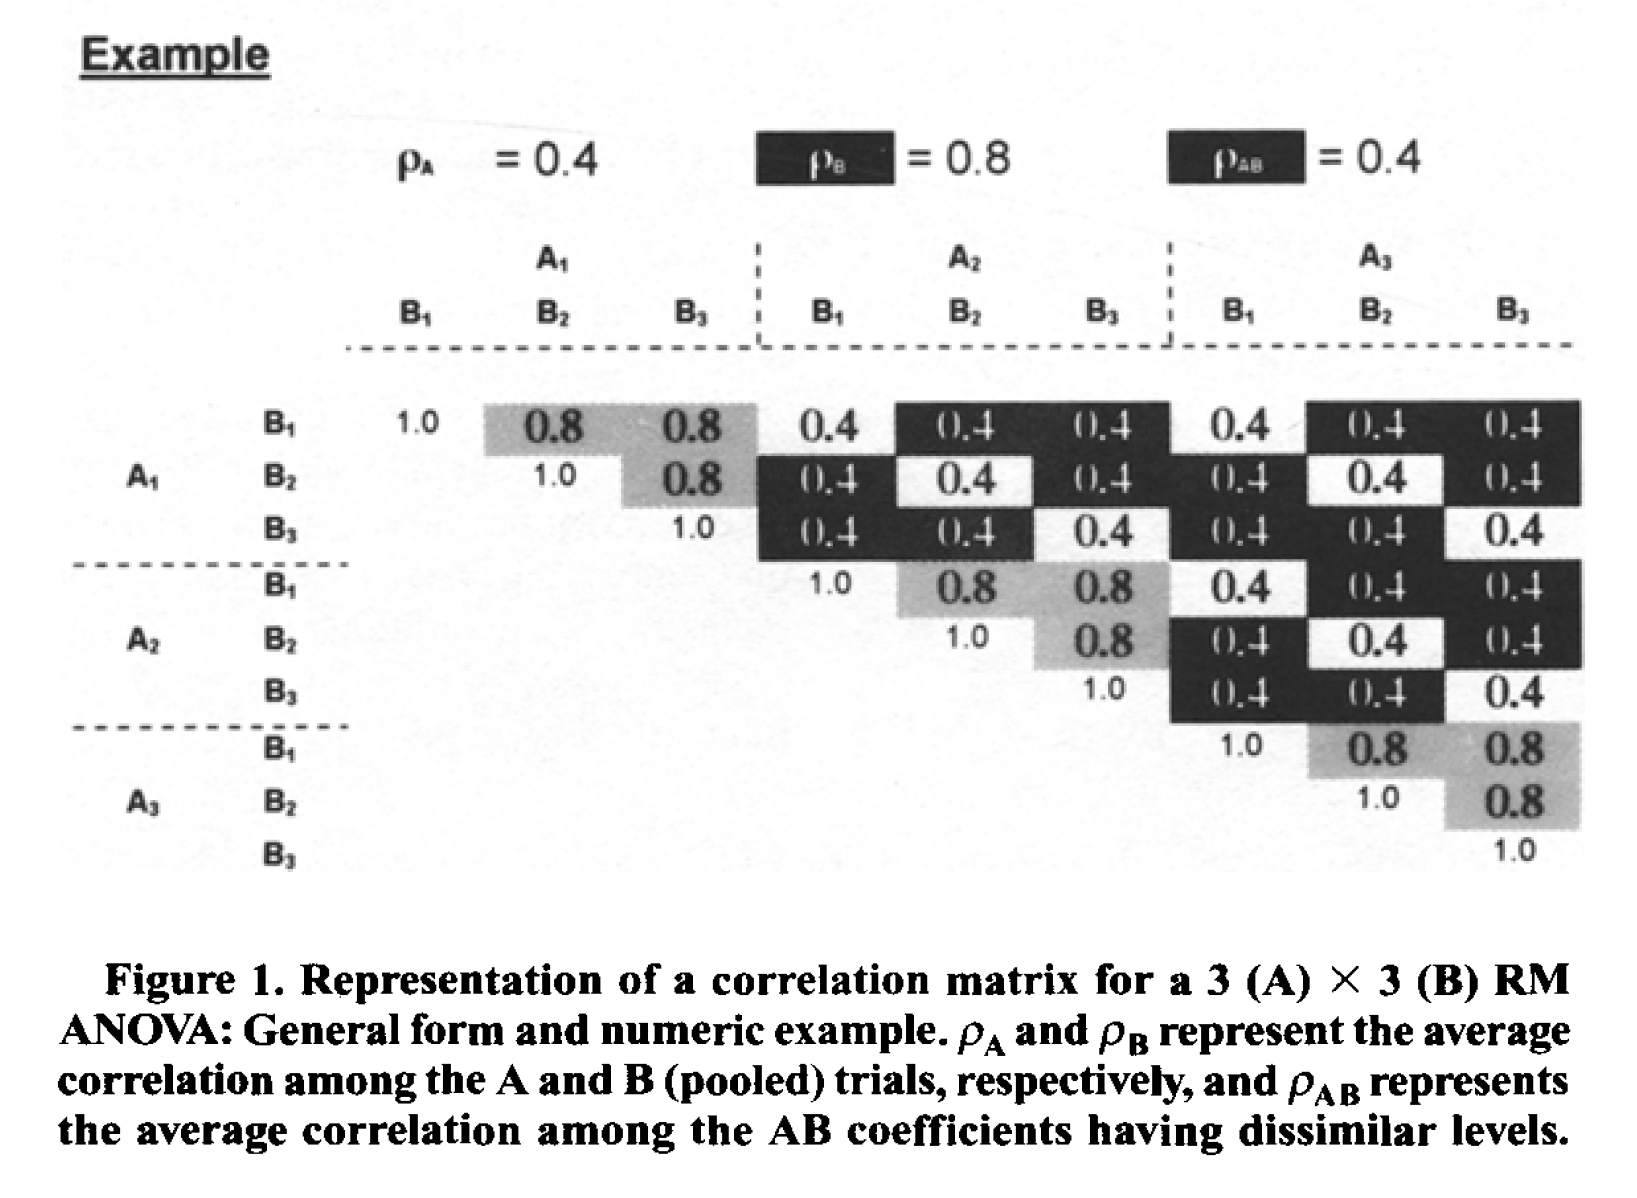
\includegraphics{screenshots/PS2000.png}

Variances were set to 1 (so all covariance matrices in their simulations were identical). In this specific example, the white fields are related to the correlation for the A main effect (these cells have the same level for B, but different levels of A). The grey cells are related to the main effect of B (the cells have the same level of A, but different levels of B). Finally, the black cells are related to the AxB interaction (they have different levels of A and B). The diagonal (all 1) relate to cells with the same levels of A and B.

Potvin \& Schulz (2000) examine power for 2x2 within ANOVA designs and develop approximations of the error variance. For a design with 2 within factors (A and B) these are:

For the main effect of A:
\(\sigma _ { e } ^ { 2 } = \sigma ^ { 2 } ( 1 - \overline { \rho } _ { A } ) + \sigma ^ { 2 } ( q - 1 ) ( \overline { \rho } _ { B } - \overline { \rho } _ { AB } )\)

For the main effectof B:
\(\sigma _ { e } ^ { 2 } = \sigma ^ { 2 } ( 1 - \overline { \rho } _ { B } ) + \sigma ^ { 2 } ( p - 1 ) ( \overline { \rho } _ { A } - \overline { \rho } _ { A B } )\)

For the interaction between A and B:
\(\sigma _ { e } ^ { 2 } = \sigma ^ { 2 } ( 1 - \rho _ { \max } ) - \sigma ^ { 2 } ( \overline { \rho } _ { \min } - \overline { \rho } _ { AB } )\)

We first simulate a within subjects 2x2 ANOVA design.

\begin{Shaded}
\begin{Highlighting}[]
\NormalTok{mu =}\StringTok{ }\KeywordTok{c}\NormalTok{(}\DecValTok{2}\NormalTok{,}\DecValTok{1}\NormalTok{,}\DecValTok{4}\NormalTok{,}\DecValTok{2}\NormalTok{) }
\NormalTok{n <-}\StringTok{ }\DecValTok{20}
\NormalTok{sd <-}\StringTok{ }\DecValTok{5}
\NormalTok{r <-}\StringTok{ }\KeywordTok{c}\NormalTok{(}
  \FloatTok{0.8}\NormalTok{, }\FloatTok{0.5}\NormalTok{, }\FloatTok{0.4}\NormalTok{,}
       \FloatTok{0.4}\NormalTok{, }\FloatTok{0.5}\NormalTok{,}
            \FloatTok{0.8}
\NormalTok{  )}
\NormalTok{string =}\StringTok{ "2w*2w"}
\NormalTok{labelnames =}\StringTok{ }\KeywordTok{c}\NormalTok{(}\StringTok{"A"}\NormalTok{, }\StringTok{"a1"}\NormalTok{, }\StringTok{"a2"}\NormalTok{, }\StringTok{"B"}\NormalTok{, }\StringTok{"b1"}\NormalTok{, }\StringTok{"b2"}\NormalTok{)}
\NormalTok{design_result <-}\StringTok{ }\KeywordTok{ANOVA_design}\NormalTok{(}\DataTypeTok{design =}\NormalTok{ string,}
                              \DataTypeTok{n =}\NormalTok{ n, }
                              \DataTypeTok{mu =}\NormalTok{ mu, }
                              \DataTypeTok{sd =}\NormalTok{ sd, }
                              \DataTypeTok{r =}\NormalTok{ r, }
                              \DataTypeTok{labelnames =}\NormalTok{ labelnames)}
\end{Highlighting}
\end{Shaded}

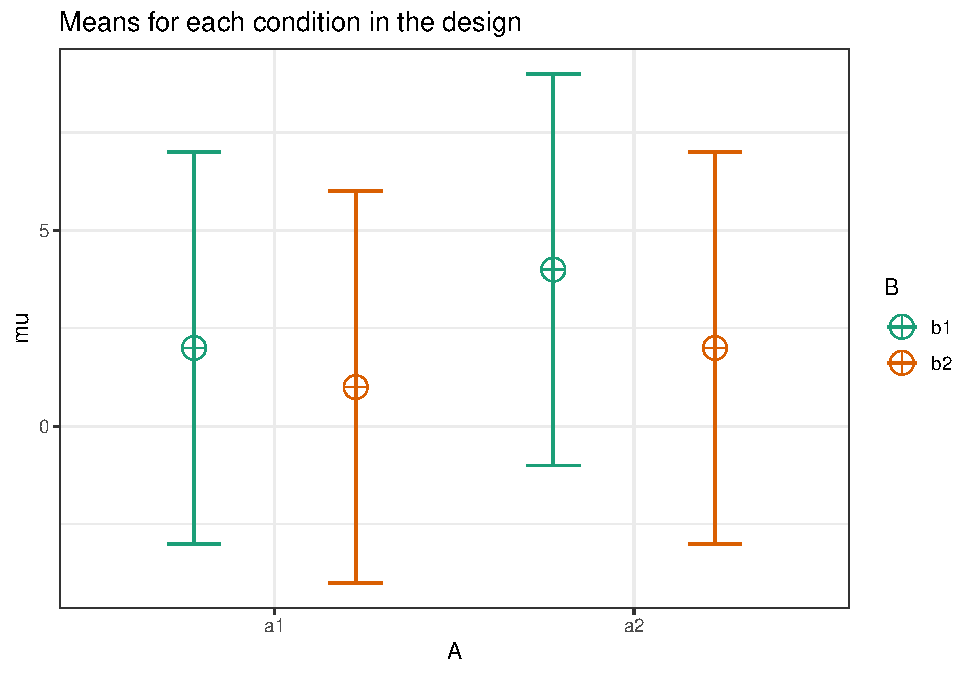
\includegraphics{SuperpowerValidation_files/figure-latex/unnamed-chunk-92-1.pdf}

\begin{Shaded}
\begin{Highlighting}[]
\NormalTok{simulation_result <-}\StringTok{ }\KeywordTok{ANOVA_power}\NormalTok{(design_result, }\DataTypeTok{alpha_level =} \FloatTok{0.05}\NormalTok{, }\DataTypeTok{nsims =}\NormalTok{ nsims)}
\end{Highlighting}
\end{Shaded}

\begin{verbatim}
## Power and Effect sizes for ANOVA tests
##           power effect_size
## anova_A      31      0.1433
## anova_B      65      0.2631
## anova_A:B    24      0.1165
## 
## Power and Effect sizes for contrasts
##                       power effect_size
## p_A_a1_B_b1_A_a1_B_b2    23    -0.34478
## p_A_a1_B_b1_A_a2_B_b1    42     0.41916
## p_A_a1_B_b1_A_a2_B_b2     7     0.01247
## p_A_a1_B_b2_A_a2_B_b1    65     0.58137
## p_A_a1_B_b2_A_a2_B_b2    15     0.22130
## p_A_a2_B_b1_A_a2_B_b2    80    -0.64982
## 
## Within-Subject Factors Included: Check MANOVA Results
\end{verbatim}

We can use the \texttt{ANOVA\_exact} function to evaluate this design.

\begin{Shaded}
\begin{Highlighting}[]
\NormalTok{power_res <-}\StringTok{ }\KeywordTok{ANOVA_exact}\NormalTok{(}\DataTypeTok{design_result =}\NormalTok{ design_result)}
\end{Highlighting}
\end{Shaded}

\begin{verbatim}
## Power and Effect sizes for ANOVA tests
##     power partial_eta_squared cohen_f non_centrality
## A   26.92              0.0952  0.3244              2
## B   64.23              0.2400  0.5620              6
## A:B 26.92              0.0952  0.3244              2
## 
## Power and Effect sizes for contrasts
##                       power effect_size
## p_A_a1_B_b1_A_a1_B_b2 26.92     -0.3162
## p_A_a1_B_b1_A_a2_B_b1 39.70      0.4000
## p_A_a1_B_b1_A_a2_B_b2  5.00      0.0000
## p_A_a1_B_b2_A_a2_B_b1 64.23      0.5477
## p_A_a1_B_b2_A_a2_B_b2 13.60      0.2000
## p_A_a2_B_b1_A_a2_B_b2 76.52     -0.6325
\end{verbatim}

\begin{Shaded}
\begin{Highlighting}[]
\NormalTok{power_res}\OperatorTok{$}\NormalTok{power_A}
\end{Highlighting}
\end{Shaded}

\begin{verbatim}
## NULL
\end{verbatim}

\begin{Shaded}
\begin{Highlighting}[]
\NormalTok{power_res}\OperatorTok{$}\NormalTok{power_B}
\end{Highlighting}
\end{Shaded}

\begin{verbatim}
## NULL
\end{verbatim}

\begin{Shaded}
\begin{Highlighting}[]
\NormalTok{power_res}\OperatorTok{$}\NormalTok{power_AB}
\end{Highlighting}
\end{Shaded}

\begin{verbatim}
## NULL
\end{verbatim}

We can use the code by Abelson (2019) to produce the same results.

\begin{Shaded}
\begin{Highlighting}[]
\KeywordTok{win2F}\NormalTok{(}\DataTypeTok{m1.1=}\DecValTok{2}\NormalTok{, }\DataTypeTok{m2.1=}\DecValTok{1}\NormalTok{, }\DataTypeTok{m1.2=}\DecValTok{4}\NormalTok{, }\DataTypeTok{m2.2=}\DecValTok{2}\NormalTok{, }
      \DataTypeTok{s1.1=}\DecValTok{5}\NormalTok{, }\DataTypeTok{s2.1=}\DecValTok{5}\NormalTok{, }\DataTypeTok{s1.2=}\DecValTok{5}\NormalTok{, }\DataTypeTok{s2.2=}\DecValTok{5}\NormalTok{, }
      \DataTypeTok{r12=}\FloatTok{0.8}\NormalTok{, }\DataTypeTok{r13=}\FloatTok{0.5}\NormalTok{, }\DataTypeTok{r14=}\FloatTok{0.4}\NormalTok{, }
               \DataTypeTok{r23=}\FloatTok{0.4}\NormalTok{, }\DataTypeTok{r24=}\FloatTok{0.5}\NormalTok{, }
                        \DataTypeTok{r34=}\FloatTok{0.8}\NormalTok{,}
      \DataTypeTok{n=}\DecValTok{20}\NormalTok{)}
\end{Highlighting}
\end{Shaded}

\hypertarget{power-curves}{%
\chapter{Power curves}\label{power-curves}}

Power is calculated for a specific value of an effect size, alpha level, and sample size. Because you often do not know the true effect size, it often makes more sense to think of the power curve as a function of the size of the effect. Although power curves can be calculated based on simulations for any design, we will use the analytic solution to calculate the power of ANOVA designs because these calculations are much faster. The basic approach is to calculate power for a specific pattern of means, a specific effect size, a given alpha level, and a specific pattern of correlations. This is one example:

\begin{Shaded}
\begin{Highlighting}[]
\CommentTok{#2x2 design}
\NormalTok{string =}\StringTok{ "2w*2w"}
\NormalTok{mu =}\StringTok{ }\KeywordTok{c}\NormalTok{(}\DecValTok{0}\NormalTok{,}\DecValTok{0}\NormalTok{,}\DecValTok{0}\NormalTok{,}\FloatTok{0.5}\NormalTok{)}
\NormalTok{n <-}\StringTok{ }\DecValTok{20}
\NormalTok{sd <-}\StringTok{ }\DecValTok{1}
\NormalTok{r <-}\StringTok{ }\FloatTok{0.5}
\NormalTok{labelnames =}\StringTok{ }\KeywordTok{c}\NormalTok{(}\StringTok{"A"}\NormalTok{, }\StringTok{"a1"}\NormalTok{, }\StringTok{"a2"}\NormalTok{, }\StringTok{"B"}\NormalTok{, }\StringTok{"b1"}\NormalTok{, }\StringTok{"b2"}\NormalTok{)}
\NormalTok{design_result <-}\StringTok{ }\KeywordTok{ANOVA_design}\NormalTok{(}\DataTypeTok{design =}\NormalTok{ string,}
                              \DataTypeTok{n =}\NormalTok{ n, }
                              \DataTypeTok{mu =}\NormalTok{ mu, }
                              \DataTypeTok{sd =}\NormalTok{ sd, }
                              \DataTypeTok{r =}\NormalTok{ r, }
                              \DataTypeTok{labelnames =}\NormalTok{ labelnames)}
\end{Highlighting}
\end{Shaded}

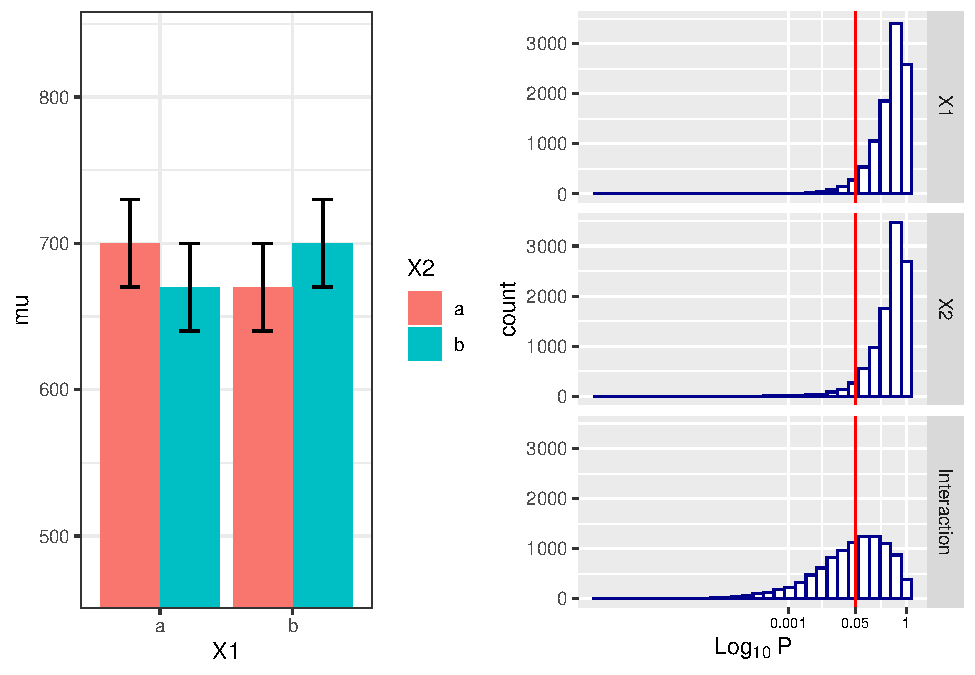
\includegraphics{SuperpowerValidation_files/figure-latex/unnamed-chunk-95-1.pdf}

\begin{Shaded}
\begin{Highlighting}[]
\NormalTok{power_res <-}\StringTok{ }\KeywordTok{ANOVA_exact}\NormalTok{(design_result)}
\end{Highlighting}
\end{Shaded}

\begin{verbatim}
## Power and Effect sizes for ANOVA tests
##     power partial_eta_squared cohen_f non_centrality
## A   32.36              0.1163  0.3627            2.5
## B   32.36              0.1163  0.3627            2.5
## A:B 32.36              0.1163  0.3627            2.5
## 
## Power and Effect sizes for contrasts
##                       power effect_size
## p_A_a1_B_b1_A_a1_B_b2  5.00         0.0
## p_A_a1_B_b1_A_a2_B_b1  5.00         0.0
## p_A_a1_B_b1_A_a2_B_b2 56.45         0.5
## p_A_a1_B_b2_A_a2_B_b1  5.00         0.0
## p_A_a1_B_b2_A_a2_B_b2 56.45         0.5
## p_A_a2_B_b1_A_a2_B_b2 56.45         0.5
\end{verbatim}

\begin{Shaded}
\begin{Highlighting}[]
\NormalTok{power_res}\OperatorTok{$}\NormalTok{main_results}
\end{Highlighting}
\end{Shaded}

\begin{verbatim}
##     power partial_eta_squared cohen_f non_centrality
## A   32.36              0.1163  0.3627            2.5
## B   32.36              0.1163  0.3627            2.5
## A:B 32.36              0.1163  0.3627            2.5
\end{verbatim}

We can make these calculations for a range of sample sizes, to get a power curve. We created a simple function that performs these calculations across a range of sample sizes (from n = 2 to max\_, a variable you can specify in the function).

\begin{Shaded}
\begin{Highlighting}[]
\NormalTok{p_a <-}\StringTok{ }\KeywordTok{plot_power}\NormalTok{(design_result,}
                      \DataTypeTok{max_n =} \DecValTok{50}\NormalTok{)}
\end{Highlighting}
\end{Shaded}

\includegraphics{SuperpowerValidation_files/figure-latex/unnamed-chunk-96-1.pdf}

\hypertarget{explore-increase-in-effect-size-for-moderated-interactions.}{%
\chapter{Explore increase in effect size for moderated interactions.}\label{explore-increase-in-effect-size-for-moderated-interactions.}}

The design has means 0, 0, 0, 0, with one cell increasing by 0.1, up to 0, 0, 0, 0.5. The standard deviation is set to 1. The correlation between all variables is 0.5.

\begin{Shaded}
\begin{Highlighting}[]
\NormalTok{string <-}\StringTok{ "2w*2w"}
\NormalTok{labelnames =}\StringTok{ }\KeywordTok{c}\NormalTok{(}\StringTok{"A"}\NormalTok{, }\StringTok{"a1"}\NormalTok{, }\StringTok{"a2"}\NormalTok{, }\StringTok{"B"}\NormalTok{, }\StringTok{"b1"}\NormalTok{, }\StringTok{"b2"}\NormalTok{)}
\NormalTok{design_result <-}\StringTok{ }\KeywordTok{ANOVA_design}\NormalTok{(}\DataTypeTok{design =}\NormalTok{ string,}
                              \DataTypeTok{n =} \DecValTok{20}\NormalTok{, }
                              \DataTypeTok{mu =} \KeywordTok{c}\NormalTok{(}\DecValTok{0}\NormalTok{,}\DecValTok{0}\NormalTok{,}\DecValTok{0}\NormalTok{,}\FloatTok{0.0}\NormalTok{), }
                              \DataTypeTok{sd =} \DecValTok{1}\NormalTok{, }
                              \DataTypeTok{r =} \FloatTok{0.5}\NormalTok{, }
                              \DataTypeTok{labelnames =}\NormalTok{ labelnames)}
\end{Highlighting}
\end{Shaded}

\includegraphics{SuperpowerValidation_files/figure-latex/unnamed-chunk-97-1.pdf}

\begin{Shaded}
\begin{Highlighting}[]
\NormalTok{p_a <-}\StringTok{ }\KeywordTok{plot_power}\NormalTok{(design_result,}
                      \DataTypeTok{max_n =} \DecValTok{100}\NormalTok{)}
\end{Highlighting}
\end{Shaded}

\includegraphics{SuperpowerValidation_files/figure-latex/unnamed-chunk-97-2.pdf}

\begin{Shaded}
\begin{Highlighting}[]
\NormalTok{design_result <-}\StringTok{ }\KeywordTok{ANOVA_design}\NormalTok{(}\DataTypeTok{design =}\NormalTok{ string,}
                              \DataTypeTok{n =} \DecValTok{20}\NormalTok{, }
                              \DataTypeTok{mu =} \KeywordTok{c}\NormalTok{(}\DecValTok{0}\NormalTok{,}\DecValTok{0}\NormalTok{,}\DecValTok{0}\NormalTok{,}\FloatTok{0.1}\NormalTok{), }
                              \DataTypeTok{sd =} \DecValTok{1}\NormalTok{, }
                              \DataTypeTok{r =} \FloatTok{0.5}\NormalTok{, }
                              \DataTypeTok{labelnames =}\NormalTok{ labelnames)}
\end{Highlighting}
\end{Shaded}

\includegraphics{SuperpowerValidation_files/figure-latex/unnamed-chunk-97-3.pdf}

\begin{Shaded}
\begin{Highlighting}[]
\NormalTok{p_b <-}\StringTok{ }\KeywordTok{plot_power}\NormalTok{(design_result,}
                      \DataTypeTok{max_n =} \DecValTok{100}\NormalTok{)}
\end{Highlighting}
\end{Shaded}

\includegraphics{SuperpowerValidation_files/figure-latex/unnamed-chunk-97-4.pdf}

\begin{Shaded}
\begin{Highlighting}[]
\NormalTok{design_result <-}\StringTok{ }\KeywordTok{ANOVA_design}\NormalTok{(}\DataTypeTok{design =}\NormalTok{ string,}
                              \DataTypeTok{n =} \DecValTok{20}\NormalTok{, }
                              \DataTypeTok{mu =} \KeywordTok{c}\NormalTok{(}\DecValTok{0}\NormalTok{,}\DecValTok{0}\NormalTok{,}\DecValTok{0}\NormalTok{,}\FloatTok{0.2}\NormalTok{), }
                              \DataTypeTok{sd =} \DecValTok{1}\NormalTok{, }
                              \DataTypeTok{r =} \FloatTok{0.5}\NormalTok{, }
                              \DataTypeTok{labelnames =}\NormalTok{ labelnames)}
\end{Highlighting}
\end{Shaded}

\includegraphics{SuperpowerValidation_files/figure-latex/unnamed-chunk-97-5.pdf}

\begin{Shaded}
\begin{Highlighting}[]
\NormalTok{p_c <-}\StringTok{ }\KeywordTok{plot_power}\NormalTok{(design_result,}
                      \DataTypeTok{max_n =} \DecValTok{100}\NormalTok{)}
\end{Highlighting}
\end{Shaded}

\includegraphics{SuperpowerValidation_files/figure-latex/unnamed-chunk-97-6.pdf}

\begin{Shaded}
\begin{Highlighting}[]
\NormalTok{design_result <-}\StringTok{ }\KeywordTok{ANOVA_design}\NormalTok{(}\DataTypeTok{design =}\NormalTok{ string,}
                              \DataTypeTok{n =} \DecValTok{20}\NormalTok{, }
                              \DataTypeTok{mu =} \KeywordTok{c}\NormalTok{(}\DecValTok{0}\NormalTok{,}\DecValTok{0}\NormalTok{,}\DecValTok{0}\NormalTok{,}\FloatTok{0.3}\NormalTok{), }
                              \DataTypeTok{sd =} \DecValTok{1}\NormalTok{, }
                              \DataTypeTok{r =} \FloatTok{0.5}\NormalTok{, }
                              \DataTypeTok{labelnames =}\NormalTok{ labelnames)}
\end{Highlighting}
\end{Shaded}

\includegraphics{SuperpowerValidation_files/figure-latex/unnamed-chunk-97-7.pdf}

\begin{Shaded}
\begin{Highlighting}[]
\NormalTok{p_d <-}\StringTok{ }\KeywordTok{plot_power}\NormalTok{(design_result,}
                      \DataTypeTok{max_n =} \DecValTok{100}\NormalTok{)}
\end{Highlighting}
\end{Shaded}

\includegraphics{SuperpowerValidation_files/figure-latex/unnamed-chunk-97-8.pdf}

\begin{Shaded}
\begin{Highlighting}[]
\NormalTok{design_result <-}\StringTok{ }\KeywordTok{ANOVA_design}\NormalTok{(}\DataTypeTok{design =}\NormalTok{ string,}
                              \DataTypeTok{n =} \DecValTok{20}\NormalTok{, }
                              \DataTypeTok{mu =} \KeywordTok{c}\NormalTok{(}\DecValTok{0}\NormalTok{,}\DecValTok{0}\NormalTok{,}\DecValTok{0}\NormalTok{,}\FloatTok{0.4}\NormalTok{), }
                              \DataTypeTok{sd =} \DecValTok{1}\NormalTok{, }
                              \DataTypeTok{r =} \FloatTok{0.5}\NormalTok{, }
                              \DataTypeTok{labelnames =}\NormalTok{ labelnames)}
\end{Highlighting}
\end{Shaded}

\includegraphics{SuperpowerValidation_files/figure-latex/unnamed-chunk-97-9.pdf}

\begin{Shaded}
\begin{Highlighting}[]
\NormalTok{p_e <-}\StringTok{ }\KeywordTok{plot_power}\NormalTok{(design_result,}
                      \DataTypeTok{max_n =} \DecValTok{100}\NormalTok{)}
\end{Highlighting}
\end{Shaded}

\includegraphics{SuperpowerValidation_files/figure-latex/unnamed-chunk-97-10.pdf}

\begin{Shaded}
\begin{Highlighting}[]
\NormalTok{design_result <-}\StringTok{ }\KeywordTok{ANOVA_design}\NormalTok{(}\DataTypeTok{design =}\NormalTok{ string,}
                              \DataTypeTok{n =} \DecValTok{20}\NormalTok{, }
                              \DataTypeTok{mu =} \KeywordTok{c}\NormalTok{(}\DecValTok{0}\NormalTok{,}\DecValTok{0}\NormalTok{,}\DecValTok{0}\NormalTok{,}\FloatTok{0.5}\NormalTok{), }
                              \DataTypeTok{sd =} \DecValTok{1}\NormalTok{, }
                              \DataTypeTok{r =} \FloatTok{0.5}\NormalTok{, }
                              \DataTypeTok{labelnames =}\NormalTok{ labelnames)}
\end{Highlighting}
\end{Shaded}

\includegraphics{SuperpowerValidation_files/figure-latex/unnamed-chunk-97-11.pdf}

\begin{Shaded}
\begin{Highlighting}[]
\NormalTok{p_f <-}\StringTok{ }\KeywordTok{plot_power}\NormalTok{(design_result,}
                      \DataTypeTok{max_n =} \DecValTok{100}\NormalTok{)}
\end{Highlighting}
\end{Shaded}

\includegraphics{SuperpowerValidation_files/figure-latex/unnamed-chunk-97-12.pdf}

\begin{Shaded}
\begin{Highlighting}[]
\CommentTok{# Create long format dataframe }
\CommentTok{#zzz <- rbind(p_a$power_df, p_b$power_df, p_c$power_df, p_d$power_df, p_e$power_df, p_f$power_df)}
\CommentTok{#zzz <- cbind(zzz,seq(1,length(zzz$design)))}
\CommentTok{#colnames(zzz)[1] <- "design"}
\CommentTok{#colnames(zzz)[6] <- "ID"}
\CommentTok{#zzz <- melt(zzz, id.vars = c("ID", "design", "n_vec"), measure.vars = c("power_A", "power_B", "power_AB"))}
\CommentTok{# Plot data using facets, split by factors and interaction, and design}
\CommentTok{#ggplot(data=zzz, aes(x = n_vec, y = value)) +}
\CommentTok{#  geom_line( size=1.5) +}
\CommentTok{#  scale_x_continuous(limits = c(0, max(zzz$n_vec))) + }
\CommentTok{#  scale_y_continuous(limits = c(0, 100)) +}
\CommentTok{#  theme_bw() +}
\CommentTok{#  labs(x="Sample size", y = "Power") +}
\CommentTok{#  facet_grid(design~variable)}
\end{Highlighting}
\end{Shaded}

\hypertarget{explore-increase-in-effect-size-for-cross-over-interactions.}{%
\section{Explore increase in effect size for cross-over interactions.}\label{explore-increase-in-effect-size-for-cross-over-interactions.}}

The design has means 0, 0, 0, 0, with two cells increasing by 0.1, up to 0.5, 0, 0, 0.5. The standard deviation is set to 1. The correlation between all variables is 0.5.

\begin{Shaded}
\begin{Highlighting}[]
\NormalTok{design_result <-}\StringTok{ }\KeywordTok{ANOVA_design}\NormalTok{(}\DataTypeTok{design =}\NormalTok{ string,}
                              \DataTypeTok{n =} \DecValTok{20}\NormalTok{, }
                              \DataTypeTok{mu =} \KeywordTok{c}\NormalTok{(}\DecValTok{0}\NormalTok{,}\DecValTok{0}\NormalTok{,}\DecValTok{0}\NormalTok{,}\FloatTok{0.0}\NormalTok{), }
                              \DataTypeTok{sd =} \DecValTok{1}\NormalTok{, }
                              \DataTypeTok{r =} \FloatTok{0.5}\NormalTok{, }
                              \DataTypeTok{labelnames =}\NormalTok{ labelnames)}
\end{Highlighting}
\end{Shaded}

\includegraphics{SuperpowerValidation_files/figure-latex/unnamed-chunk-98-1.pdf}

\begin{Shaded}
\begin{Highlighting}[]
\NormalTok{p_a <-}\StringTok{ }\KeywordTok{plot_power}\NormalTok{(design_result,}
                      \DataTypeTok{max_n =} \DecValTok{100}\NormalTok{)}
\end{Highlighting}
\end{Shaded}

\includegraphics{SuperpowerValidation_files/figure-latex/unnamed-chunk-98-2.pdf}

\begin{Shaded}
\begin{Highlighting}[]
\NormalTok{design_result <-}\StringTok{ }\KeywordTok{ANOVA_design}\NormalTok{(}\DataTypeTok{design =}\NormalTok{ string,}
                              \DataTypeTok{n =} \DecValTok{20}\NormalTok{, }
                              \DataTypeTok{mu =} \KeywordTok{c}\NormalTok{(}\FloatTok{0.1}\NormalTok{,}\DecValTok{0}\NormalTok{,}\DecValTok{0}\NormalTok{,}\FloatTok{0.1}\NormalTok{), }
                              \DataTypeTok{sd =} \DecValTok{1}\NormalTok{, }
                              \DataTypeTok{r =} \FloatTok{0.5}\NormalTok{, }
                              \DataTypeTok{labelnames =}\NormalTok{ labelnames)}
\end{Highlighting}
\end{Shaded}

\includegraphics{SuperpowerValidation_files/figure-latex/unnamed-chunk-98-3.pdf}

\begin{Shaded}
\begin{Highlighting}[]
\NormalTok{p_b <-}\StringTok{ }\KeywordTok{plot_power}\NormalTok{(design_result,}
                      \DataTypeTok{max_n =} \DecValTok{100}\NormalTok{)}
\end{Highlighting}
\end{Shaded}

\includegraphics{SuperpowerValidation_files/figure-latex/unnamed-chunk-98-4.pdf}

\begin{Shaded}
\begin{Highlighting}[]
\NormalTok{design_result <-}\StringTok{ }\KeywordTok{ANOVA_design}\NormalTok{(}\DataTypeTok{design =}\NormalTok{ string,}
                              \DataTypeTok{n =} \DecValTok{20}\NormalTok{, }
                              \DataTypeTok{mu =} \KeywordTok{c}\NormalTok{(}\FloatTok{0.2}\NormalTok{,}\DecValTok{0}\NormalTok{,}\DecValTok{0}\NormalTok{,}\FloatTok{0.2}\NormalTok{), }
                              \DataTypeTok{sd =} \DecValTok{1}\NormalTok{, }
                              \DataTypeTok{r =} \FloatTok{0.5}\NormalTok{, }
                              \DataTypeTok{labelnames =}\NormalTok{ labelnames)}
\end{Highlighting}
\end{Shaded}

\includegraphics{SuperpowerValidation_files/figure-latex/unnamed-chunk-98-5.pdf}

\begin{Shaded}
\begin{Highlighting}[]
\NormalTok{p_c <-}\StringTok{ }\KeywordTok{plot_power}\NormalTok{(design_result,}
                      \DataTypeTok{max_n =} \DecValTok{100}\NormalTok{)}
\end{Highlighting}
\end{Shaded}

\includegraphics{SuperpowerValidation_files/figure-latex/unnamed-chunk-98-6.pdf}

\begin{Shaded}
\begin{Highlighting}[]
\NormalTok{design_result <-}\StringTok{ }\KeywordTok{ANOVA_design}\NormalTok{(}\DataTypeTok{design =}\NormalTok{ string,}
                              \DataTypeTok{n =} \DecValTok{20}\NormalTok{, }
                              \DataTypeTok{mu =} \KeywordTok{c}\NormalTok{(}\FloatTok{0.3}\NormalTok{,}\DecValTok{0}\NormalTok{,}\DecValTok{0}\NormalTok{,}\FloatTok{0.3}\NormalTok{), }
                              \DataTypeTok{sd =} \DecValTok{1}\NormalTok{, }
                              \DataTypeTok{r =} \FloatTok{0.5}\NormalTok{, }
                              \DataTypeTok{labelnames =}\NormalTok{ labelnames)}
\end{Highlighting}
\end{Shaded}

\includegraphics{SuperpowerValidation_files/figure-latex/unnamed-chunk-98-7.pdf}

\begin{Shaded}
\begin{Highlighting}[]
\NormalTok{p_d <-}\StringTok{ }\KeywordTok{plot_power}\NormalTok{(design_result,}
                      \DataTypeTok{max_n =} \DecValTok{100}\NormalTok{)}
\end{Highlighting}
\end{Shaded}

\includegraphics{SuperpowerValidation_files/figure-latex/unnamed-chunk-98-8.pdf}

\begin{Shaded}
\begin{Highlighting}[]
\NormalTok{design_result <-}\StringTok{ }\KeywordTok{ANOVA_design}\NormalTok{(}\DataTypeTok{design =}\NormalTok{ string,}
                              \DataTypeTok{n =} \DecValTok{20}\NormalTok{, }
                              \DataTypeTok{mu =} \KeywordTok{c}\NormalTok{(}\FloatTok{0.4}\NormalTok{,}\DecValTok{0}\NormalTok{,}\DecValTok{0}\NormalTok{,}\FloatTok{0.4}\NormalTok{), }
                              \DataTypeTok{sd =} \DecValTok{1}\NormalTok{, }
                              \DataTypeTok{r =} \FloatTok{0.5}\NormalTok{, }
                              \DataTypeTok{labelnames =}\NormalTok{ labelnames)}
\end{Highlighting}
\end{Shaded}

\includegraphics{SuperpowerValidation_files/figure-latex/unnamed-chunk-98-9.pdf}

\begin{Shaded}
\begin{Highlighting}[]
\NormalTok{p_e <-}\StringTok{ }\KeywordTok{plot_power}\NormalTok{(design_result,}
                      \DataTypeTok{max_n =} \DecValTok{100}\NormalTok{)}
\end{Highlighting}
\end{Shaded}

\includegraphics{SuperpowerValidation_files/figure-latex/unnamed-chunk-98-10.pdf}

\begin{Shaded}
\begin{Highlighting}[]
\NormalTok{design_result <-}\StringTok{ }\KeywordTok{ANOVA_design}\NormalTok{(}\DataTypeTok{design =}\NormalTok{ string,}
                              \DataTypeTok{n =} \DecValTok{20}\NormalTok{, }
                              \DataTypeTok{mu =} \KeywordTok{c}\NormalTok{(}\FloatTok{0.5}\NormalTok{,}\DecValTok{0}\NormalTok{,}\DecValTok{0}\NormalTok{,}\FloatTok{0.5}\NormalTok{), }
                              \DataTypeTok{sd =} \DecValTok{1}\NormalTok{, }
                              \DataTypeTok{r =} \FloatTok{0.5}\NormalTok{, }
                              \DataTypeTok{labelnames =}\NormalTok{ labelnames)}
\end{Highlighting}
\end{Shaded}

\includegraphics{SuperpowerValidation_files/figure-latex/unnamed-chunk-98-11.pdf}

\begin{Shaded}
\begin{Highlighting}[]
\NormalTok{p_f <-}\StringTok{ }\KeywordTok{plot_power}\NormalTok{(design_result,}
                      \DataTypeTok{max_n =} \DecValTok{100}\NormalTok{)}
\end{Highlighting}
\end{Shaded}

\includegraphics{SuperpowerValidation_files/figure-latex/unnamed-chunk-98-12.pdf}

\hypertarget{explore-increase-in-correlation-in-moderated-interactions.}{%
\section{Explore increase in correlation in moderated interactions.}\label{explore-increase-in-correlation-in-moderated-interactions.}}

The design has means 0, 0, 0, 0.3. The standard deviation is set to 1. The correlation between all variables increases from 0.5 to 0.9.

\begin{Shaded}
\begin{Highlighting}[]
\NormalTok{string <-}\StringTok{ "2w*2w"}
\NormalTok{labelnames =}\StringTok{ }\KeywordTok{c}\NormalTok{(}\StringTok{"A"}\NormalTok{, }\StringTok{"a1"}\NormalTok{, }\StringTok{"a2"}\NormalTok{, }\StringTok{"B"}\NormalTok{, }\StringTok{"b1"}\NormalTok{, }\StringTok{"b2"}\NormalTok{)}
\NormalTok{design_result <-}\StringTok{ }\KeywordTok{ANOVA_design}\NormalTok{(}\DataTypeTok{design =}\NormalTok{ string,}
                              \DataTypeTok{n =} \DecValTok{20}\NormalTok{, }
                              \DataTypeTok{mu =} \KeywordTok{c}\NormalTok{(}\DecValTok{0}\NormalTok{,}\DecValTok{0}\NormalTok{,}\DecValTok{0}\NormalTok{,}\FloatTok{0.3}\NormalTok{), }
                              \DataTypeTok{sd =} \DecValTok{1}\NormalTok{, }
                              \DataTypeTok{r =} \FloatTok{0.0}\NormalTok{, }
                              \DataTypeTok{labelnames =}\NormalTok{ labelnames)}
\end{Highlighting}
\end{Shaded}

\includegraphics{SuperpowerValidation_files/figure-latex/unnamed-chunk-99-1.pdf}

\begin{Shaded}
\begin{Highlighting}[]
\NormalTok{p_a <-}\StringTok{ }\KeywordTok{plot_power}\NormalTok{(design_result,}
                      \DataTypeTok{max_n =} \DecValTok{100}\NormalTok{)}
\end{Highlighting}
\end{Shaded}

\includegraphics{SuperpowerValidation_files/figure-latex/unnamed-chunk-99-2.pdf}

\begin{Shaded}
\begin{Highlighting}[]
\NormalTok{design_result <-}\StringTok{ }\KeywordTok{ANOVA_design}\NormalTok{(}\DataTypeTok{design =}\NormalTok{ string,}
                              \DataTypeTok{n =} \DecValTok{20}\NormalTok{, }
                              \DataTypeTok{mu =} \KeywordTok{c}\NormalTok{(}\DecValTok{0}\NormalTok{,}\DecValTok{0}\NormalTok{,}\DecValTok{0}\NormalTok{,}\FloatTok{0.3}\NormalTok{), }
                              \DataTypeTok{sd =} \DecValTok{1}\NormalTok{, }
                              \DataTypeTok{r =} \FloatTok{0.1}\NormalTok{, }
                              \DataTypeTok{labelnames =}\NormalTok{ labelnames)}
\end{Highlighting}
\end{Shaded}

\includegraphics{SuperpowerValidation_files/figure-latex/unnamed-chunk-99-3.pdf}

\begin{Shaded}
\begin{Highlighting}[]
\NormalTok{p_b <-}\StringTok{ }\KeywordTok{plot_power}\NormalTok{(design_result,}
                      \DataTypeTok{max_n =} \DecValTok{100}\NormalTok{)}
\end{Highlighting}
\end{Shaded}

\includegraphics{SuperpowerValidation_files/figure-latex/unnamed-chunk-99-4.pdf}

\begin{Shaded}
\begin{Highlighting}[]
\NormalTok{design_result <-}\StringTok{ }\KeywordTok{ANOVA_design}\NormalTok{(}\DataTypeTok{design =}\NormalTok{ string,}
                              \DataTypeTok{n =} \DecValTok{20}\NormalTok{, }
                              \DataTypeTok{mu =} \KeywordTok{c}\NormalTok{(}\DecValTok{0}\NormalTok{,}\DecValTok{0}\NormalTok{,}\DecValTok{0}\NormalTok{,}\FloatTok{0.3}\NormalTok{), }
                              \DataTypeTok{sd =} \DecValTok{1}\NormalTok{, }
                              \DataTypeTok{r =} \FloatTok{0.3}\NormalTok{, }
                              \DataTypeTok{labelnames =}\NormalTok{ labelnames)}
\end{Highlighting}
\end{Shaded}

\includegraphics{SuperpowerValidation_files/figure-latex/unnamed-chunk-99-5.pdf}

\begin{Shaded}
\begin{Highlighting}[]
\NormalTok{p_c <-}\StringTok{ }\KeywordTok{plot_power}\NormalTok{(design_result,}
                      \DataTypeTok{max_n =} \DecValTok{100}\NormalTok{)}
\end{Highlighting}
\end{Shaded}

\includegraphics{SuperpowerValidation_files/figure-latex/unnamed-chunk-99-6.pdf}

\begin{Shaded}
\begin{Highlighting}[]
\NormalTok{design_result <-}\StringTok{ }\KeywordTok{ANOVA_design}\NormalTok{(}\DataTypeTok{design =}\NormalTok{ string,}
                              \DataTypeTok{n =} \DecValTok{20}\NormalTok{, }
                              \DataTypeTok{mu =} \KeywordTok{c}\NormalTok{(}\DecValTok{0}\NormalTok{,}\DecValTok{0}\NormalTok{,}\DecValTok{0}\NormalTok{,}\FloatTok{0.3}\NormalTok{), }
                              \DataTypeTok{sd =} \DecValTok{1}\NormalTok{, }
                              \DataTypeTok{r =} \FloatTok{0.5}\NormalTok{, }
                              \DataTypeTok{labelnames =}\NormalTok{ labelnames)}
\end{Highlighting}
\end{Shaded}

\includegraphics{SuperpowerValidation_files/figure-latex/unnamed-chunk-99-7.pdf}

\begin{Shaded}
\begin{Highlighting}[]
\NormalTok{p_d <-}\StringTok{ }\KeywordTok{plot_power}\NormalTok{(design_result,}
                      \DataTypeTok{max_n =} \DecValTok{100}\NormalTok{)}
\end{Highlighting}
\end{Shaded}

\includegraphics{SuperpowerValidation_files/figure-latex/unnamed-chunk-99-8.pdf}

\begin{Shaded}
\begin{Highlighting}[]
\NormalTok{design_result <-}\StringTok{ }\KeywordTok{ANOVA_design}\NormalTok{(}\DataTypeTok{design =}\NormalTok{ string,}
                              \DataTypeTok{n =} \DecValTok{20}\NormalTok{, }
                              \DataTypeTok{mu =} \KeywordTok{c}\NormalTok{(}\DecValTok{0}\NormalTok{,}\DecValTok{0}\NormalTok{,}\DecValTok{0}\NormalTok{,}\FloatTok{0.3}\NormalTok{), }
                              \DataTypeTok{sd =} \DecValTok{1}\NormalTok{, }
                              \DataTypeTok{r =} \FloatTok{0.7}\NormalTok{, }
                              \DataTypeTok{labelnames =}\NormalTok{ labelnames)}
\end{Highlighting}
\end{Shaded}

\includegraphics{SuperpowerValidation_files/figure-latex/unnamed-chunk-99-9.pdf}

\begin{Shaded}
\begin{Highlighting}[]
\NormalTok{p_e <-}\StringTok{ }\KeywordTok{plot_power}\NormalTok{(design_result,}
                      \DataTypeTok{max_n =} \DecValTok{100}\NormalTok{)}
\end{Highlighting}
\end{Shaded}

\includegraphics{SuperpowerValidation_files/figure-latex/unnamed-chunk-99-10.pdf}

\begin{Shaded}
\begin{Highlighting}[]
\NormalTok{design_result <-}\StringTok{ }\KeywordTok{ANOVA_design}\NormalTok{(}\DataTypeTok{design =}\NormalTok{ string,}
                              \DataTypeTok{n =} \DecValTok{20}\NormalTok{, }
                              \DataTypeTok{mu =} \KeywordTok{c}\NormalTok{(}\DecValTok{0}\NormalTok{,}\DecValTok{0}\NormalTok{,}\DecValTok{0}\NormalTok{,}\FloatTok{0.3}\NormalTok{), }
                              \DataTypeTok{sd =} \DecValTok{1}\NormalTok{, }
                              \DataTypeTok{r =} \FloatTok{0.9}\NormalTok{, }
                              \DataTypeTok{labelnames =}\NormalTok{ labelnames)}
\end{Highlighting}
\end{Shaded}

\includegraphics{SuperpowerValidation_files/figure-latex/unnamed-chunk-99-11.pdf}

\begin{Shaded}
\begin{Highlighting}[]
\NormalTok{p_f <-}\StringTok{ }\KeywordTok{plot_power}\NormalTok{(design_result,}
                      \DataTypeTok{max_n =} \DecValTok{100}\NormalTok{)}
\end{Highlighting}
\end{Shaded}

\includegraphics{SuperpowerValidation_files/figure-latex/unnamed-chunk-99-12.pdf}

\hypertarget{increasing-correlation-in-on-factor-decreases-power-in-second-factor}{%
\section{Increasing correlation in on factor decreases power in second factor}\label{increasing-correlation-in-on-factor-decreases-power-in-second-factor}}

As Potvin and Schutz (2000) write: ``The more important finding with respect to the effect of \emph{r} on power relates to the effect of the correlations associated with one factor on the power of the test of the main effect of the other factor. Specifically, if the correlations among the levels of B are larger than those within the AB matrix (i.e., \emph{r}B - \emph{r}AB \textgreater{} 0.0), there is a reduction in the power for the test of the A effect (and the test on B is similarly affected by the A correlations).''
We see this in the plots below. As the correlation of the A factor increases from 0.4 to 0.9, we see the power for the main effect of factor B decreases.

\begin{Shaded}
\begin{Highlighting}[]
\NormalTok{string <-}\StringTok{ "2w*2w"}
\NormalTok{labelnames =}\StringTok{ }\KeywordTok{c}\NormalTok{(}\StringTok{"A"}\NormalTok{, }\StringTok{"a1"}\NormalTok{, }\StringTok{"a2"}\NormalTok{, }\StringTok{"B"}\NormalTok{, }\StringTok{"b1"}\NormalTok{, }\StringTok{"b2"}\NormalTok{)}
\NormalTok{design_result <-}\StringTok{ }\KeywordTok{ANOVA_design}\NormalTok{(}\DataTypeTok{design =}\NormalTok{ string,}
                              \DataTypeTok{n =} \DecValTok{20}\NormalTok{, }
                              \DataTypeTok{mu =} \KeywordTok{c}\NormalTok{(}\DecValTok{0}\NormalTok{,}\DecValTok{0}\NormalTok{,}\DecValTok{0}\NormalTok{,}\FloatTok{0.3}\NormalTok{), }
                              \DataTypeTok{sd =} \DecValTok{1}\NormalTok{, }
\NormalTok{                              r <-}\StringTok{ }\KeywordTok{c}\NormalTok{(}
                                \FloatTok{0.4}\NormalTok{, }\FloatTok{0.4}\NormalTok{, }\FloatTok{0.4}\NormalTok{,}
                                \FloatTok{0.4}\NormalTok{, }\FloatTok{0.4}\NormalTok{,}
                                \FloatTok{0.4}\NormalTok{),}
                              \DataTypeTok{labelnames =}\NormalTok{ labelnames)}
\end{Highlighting}
\end{Shaded}

\includegraphics{SuperpowerValidation_files/figure-latex/unnamed-chunk-100-1.pdf}

\begin{Shaded}
\begin{Highlighting}[]
\NormalTok{p_a <-}\StringTok{ }\KeywordTok{plot_power}\NormalTok{(design_result,}
                      \DataTypeTok{max_n =} \DecValTok{100}\NormalTok{)}
\end{Highlighting}
\end{Shaded}

\includegraphics{SuperpowerValidation_files/figure-latex/unnamed-chunk-100-2.pdf}

\begin{Shaded}
\begin{Highlighting}[]
\NormalTok{design_result <-}\StringTok{ }\KeywordTok{ANOVA_design}\NormalTok{(}\DataTypeTok{design =}\NormalTok{ string,}
                              \DataTypeTok{n =} \DecValTok{20}\NormalTok{, }
                              \DataTypeTok{mu =} \KeywordTok{c}\NormalTok{(}\DecValTok{0}\NormalTok{,}\DecValTok{0}\NormalTok{,}\DecValTok{0}\NormalTok{,}\FloatTok{0.3}\NormalTok{), }
                              \DataTypeTok{sd =} \DecValTok{1}\NormalTok{, }
\NormalTok{                              r <-}\StringTok{ }\KeywordTok{c}\NormalTok{(}
                                \FloatTok{0.5}\NormalTok{, }\FloatTok{0.4}\NormalTok{, }\FloatTok{0.4}\NormalTok{,}
                                \FloatTok{0.4}\NormalTok{, }\FloatTok{0.4}\NormalTok{,}
                                \FloatTok{0.5}\NormalTok{),}
                              \DataTypeTok{labelnames =}\NormalTok{ labelnames)}
\end{Highlighting}
\end{Shaded}

\includegraphics{SuperpowerValidation_files/figure-latex/unnamed-chunk-100-3.pdf}

\begin{Shaded}
\begin{Highlighting}[]
\NormalTok{p_b <-}\StringTok{ }\KeywordTok{plot_power}\NormalTok{(design_result,}
                      \DataTypeTok{max_n =} \DecValTok{100}\NormalTok{)}
\end{Highlighting}
\end{Shaded}

\includegraphics{SuperpowerValidation_files/figure-latex/unnamed-chunk-100-4.pdf}

\begin{Shaded}
\begin{Highlighting}[]
\NormalTok{design_result <-}\StringTok{ }\KeywordTok{ANOVA_design}\NormalTok{(}\DataTypeTok{design =}\NormalTok{ string,}
                              \DataTypeTok{n =} \DecValTok{20}\NormalTok{, }
                              \DataTypeTok{mu =} \KeywordTok{c}\NormalTok{(}\DecValTok{0}\NormalTok{,}\DecValTok{0}\NormalTok{,}\DecValTok{0}\NormalTok{,}\FloatTok{0.3}\NormalTok{), }
                              \DataTypeTok{sd =} \DecValTok{1}\NormalTok{, }
\NormalTok{                              r <-}\StringTok{ }\KeywordTok{c}\NormalTok{(}
                                \FloatTok{0.6}\NormalTok{, }\FloatTok{0.4}\NormalTok{, }\FloatTok{0.4}\NormalTok{,}
                                \FloatTok{0.4}\NormalTok{, }\FloatTok{0.4}\NormalTok{,}
                                \FloatTok{0.6}\NormalTok{),}
                              \DataTypeTok{labelnames =}\NormalTok{ labelnames)}
\end{Highlighting}
\end{Shaded}

\includegraphics{SuperpowerValidation_files/figure-latex/unnamed-chunk-100-5.pdf}

\begin{Shaded}
\begin{Highlighting}[]
\NormalTok{p_c <-}\StringTok{ }\KeywordTok{plot_power}\NormalTok{(design_result,}
                      \DataTypeTok{max_n =} \DecValTok{100}\NormalTok{)}
\end{Highlighting}
\end{Shaded}

\includegraphics{SuperpowerValidation_files/figure-latex/unnamed-chunk-100-6.pdf}

\begin{Shaded}
\begin{Highlighting}[]
\NormalTok{design_result <-}\StringTok{ }\KeywordTok{ANOVA_design}\NormalTok{(}\DataTypeTok{design =}\NormalTok{ string,}
                              \DataTypeTok{n =} \DecValTok{20}\NormalTok{, }
                              \DataTypeTok{mu =} \KeywordTok{c}\NormalTok{(}\DecValTok{0}\NormalTok{,}\DecValTok{0}\NormalTok{,}\DecValTok{0}\NormalTok{,}\FloatTok{0.3}\NormalTok{), }
                              \DataTypeTok{sd =} \DecValTok{1}\NormalTok{, }
\NormalTok{                              r <-}\StringTok{ }\KeywordTok{c}\NormalTok{(}
                                \FloatTok{0.7}\NormalTok{, }\FloatTok{0.4}\NormalTok{, }\FloatTok{0.4}\NormalTok{,}
                                \FloatTok{0.4}\NormalTok{, }\FloatTok{0.4}\NormalTok{,}
                                \FloatTok{0.7}\NormalTok{), }
                              \DataTypeTok{labelnames =}\NormalTok{ labelnames)}
\end{Highlighting}
\end{Shaded}

\includegraphics{SuperpowerValidation_files/figure-latex/unnamed-chunk-100-7.pdf}

\begin{Shaded}
\begin{Highlighting}[]
\NormalTok{p_d <-}\StringTok{ }\KeywordTok{plot_power}\NormalTok{(design_result,}
                      \DataTypeTok{max_n =} \DecValTok{100}\NormalTok{)}
\end{Highlighting}
\end{Shaded}

\includegraphics{SuperpowerValidation_files/figure-latex/unnamed-chunk-100-8.pdf}

\begin{Shaded}
\begin{Highlighting}[]
\NormalTok{design_result <-}\StringTok{ }\KeywordTok{ANOVA_design}\NormalTok{(}\DataTypeTok{design =}\NormalTok{ string,}
                              \DataTypeTok{n =} \DecValTok{20}\NormalTok{, }
                              \DataTypeTok{mu =} \KeywordTok{c}\NormalTok{(}\DecValTok{0}\NormalTok{,}\DecValTok{0}\NormalTok{,}\DecValTok{0}\NormalTok{,}\FloatTok{0.3}\NormalTok{), }
                              \DataTypeTok{sd =} \DecValTok{1}\NormalTok{, }
\NormalTok{                              r <-}\StringTok{ }\KeywordTok{c}\NormalTok{(}
                                \FloatTok{0.8}\NormalTok{, }\FloatTok{0.4}\NormalTok{, }\FloatTok{0.4}\NormalTok{,}
                                \FloatTok{0.4}\NormalTok{, }\FloatTok{0.4}\NormalTok{,}
                                \FloatTok{0.8}\NormalTok{), }
                              \DataTypeTok{labelnames =}\NormalTok{ labelnames)}
\end{Highlighting}
\end{Shaded}

\includegraphics{SuperpowerValidation_files/figure-latex/unnamed-chunk-100-9.pdf}

\begin{Shaded}
\begin{Highlighting}[]
\NormalTok{p_e <-}\StringTok{ }\KeywordTok{plot_power}\NormalTok{(design_result,}
                      \DataTypeTok{max_n =} \DecValTok{100}\NormalTok{)}
\end{Highlighting}
\end{Shaded}

\includegraphics{SuperpowerValidation_files/figure-latex/unnamed-chunk-100-10.pdf}

\begin{Shaded}
\begin{Highlighting}[]
\NormalTok{design_result <-}\StringTok{ }\KeywordTok{ANOVA_design}\NormalTok{(}\DataTypeTok{design =}\NormalTok{ string,}
                              \DataTypeTok{n =} \DecValTok{20}\NormalTok{, }
                              \DataTypeTok{mu =} \KeywordTok{c}\NormalTok{(}\DecValTok{0}\NormalTok{,}\DecValTok{0}\NormalTok{,}\DecValTok{0}\NormalTok{,}\FloatTok{0.3}\NormalTok{), }
                              \DataTypeTok{sd =} \DecValTok{1}\NormalTok{, }
\NormalTok{                              r <-}\StringTok{ }\KeywordTok{c}\NormalTok{(}
                                \FloatTok{0.9}\NormalTok{, }\FloatTok{0.4}\NormalTok{, }\FloatTok{0.4}\NormalTok{,}
                                \FloatTok{0.4}\NormalTok{, }\FloatTok{0.4}\NormalTok{,}
                                \FloatTok{0.9}\NormalTok{), }
                              \DataTypeTok{labelnames =}\NormalTok{ labelnames)}
\end{Highlighting}
\end{Shaded}

\includegraphics{SuperpowerValidation_files/figure-latex/unnamed-chunk-100-11.pdf}

\begin{Shaded}
\begin{Highlighting}[]
\NormalTok{p_f <-}\StringTok{ }\KeywordTok{plot_power}\NormalTok{(design_result,}
                      \DataTypeTok{max_n =} \DecValTok{100}\NormalTok{)}
\end{Highlighting}
\end{Shaded}

\includegraphics{SuperpowerValidation_files/figure-latex/unnamed-chunk-100-12.pdf}

\bibliography{book.bib,packages.bib}


\end{document}
